%\pdfoutput=0
%%%%%%%%%%%%%%%%%%%%%%%%%%%%%%%%%%%%%%%%%%%%%%%%%%%%%%%%%%%%%%%%%%%
%%\documentclass[english,ngerman,headsepline,noparindent,greybox, chapterprefix=true]{bgteubner}
%
%\usepackage{graphicx}
%\usepackage{dcolumn}
%\usepackage[gen]{eurosym}
%%\usepackage{miller}
%\usepackage{contour}
%%\usepackage{fixme}
%\usepackage{nicefrac}
%\usepackage{url}
%%\usepackage{overpic}
%\usepackage{verbatim}
%%\usepackage{url}
%%\usepackage{tocloft}
%%\usepackage{cite}
%\usepackage{babelbib}
%\usepackage{psfrag}
%\usepackage[utf8]{inputenc}
%\usepackage{capt-of}
%\usepackage{ngerman}
%%\usepackage[ps2pdf,bookmarks=true,bookmarksopen=false,bookmarksnumbered=true]{hyperref}
%%\usepackage{bookmark}
%\usepackage{amsmath}
%\usepackage{xcolor}
%%**** tikz package, �bernommen von Johannes Agricola aus dem EP Skript********
%\usepackage{tikz}
%\usepackage{pgfplots}
%\usetikzlibrary{calc, babel, intersections}
%\usetikzlibrary{arrows}
%\usetikzlibrary{decorations.markings}
%\usetikzlibrary{decorations.pathreplacing}
%\usepackage[european resistors]{circuitikz}

%%%%%%%%%%%%%%%%%%%%%%%%%%%%%%%%%%%%%%%%%%%%%%%%%%%%%%%%%%%%%%%%%%
% �bernommen vom EP Skript
%%%%%%%%%%%%%%%%%%%%%%%%%%%%%%%%%%%%%%%%%%%%%%%%%%%%%%%%%%%%%%%%%%
\documentclass[11pt, twoside, a4paper]{book}

\usepackage{graphicx}
\usepackage[utf8]{inputenc}
\usepackage{ngerman}
%\usepackage{lineno}
\usepackage{verbatim}
%\usepackage{comment}
\usepackage[squaren]{SIunits}
\usepackage{amsmath}
\usepackage{amsfonts}
\usepackage{amssymb}
\usepackage{enumitem}
\usepackage{fancyhdr}
\usepackage{textcomp}
\usepackage{subcaption}
\usepackage[noadjust]{marginnote}
\usepackage{hyperref}
\usepackage{tikz}
\usepackage{pgfplots}
\usepackage{nicefrac}
\usepackage{framed}
\usetikzlibrary{calc,intersections}
\usetikzlibrary{arrows}
\usetikzlibrary{decorations.markings}
\usetikzlibrary{decorations.pathreplacing}
\makeatletter

% Data Flip Flip (DFF) shape
\pgfdeclareshape{dff}{
  % The 'minimum width' and 'minimum height' keys, not the content, determine
  % the size
  \savedanchor\northeast{%
    \pgfmathsetlength\pgf@x{\pgfshapeminwidth}%
    \pgfmathsetlength\pgf@y{\pgfshapeminheight}%
    \pgf@x=0.5\pgf@x
    \pgf@y=0.5\pgf@y
  }
  % This is redundant, but makes some things easier:
  \savedanchor\southwest{%
    \pgfmathsetlength\pgf@x{\pgfshapeminwidth}%
    \pgfmathsetlength\pgf@y{\pgfshapeminheight}%
    \pgf@x=-0.5\pgf@x
    \pgf@y=-0.5\pgf@y
  }
  % Inherit from rectangle
  \inheritanchorborder[from=rectangle]

  % Define same anchor a normal rectangle has
  \anchor{center}{\pgfpointorigin}
  \anchor{north}{\northeast \pgf@x=0pt}
  \anchor{east}{\northeast \pgf@y=0pt}
  \anchor{south}{\southwest \pgf@x=0pt}
  \anchor{west}{\southwest \pgf@y=0pt}
  \anchor{north east}{\northeast}
  \anchor{north west}{\northeast \pgf@x=-\pgf@x}
  \anchor{south west}{\southwest}
  \anchor{south east}{\southwest \pgf@x=-\pgf@x}
  \anchor{text}{
    \pgfpointorigin
    \advance\pgf@x by -.5\wd\pgfnodeparttextbox%
    \advance\pgf@y by -.5\ht\pgfnodeparttextbox%
    \advance\pgf@y by +.5\dp\pgfnodeparttextbox%
  }

  % Define anchors for signal ports
  \anchor{D}{
    \pgf@process{\northeast}%
    \pgf@x=-1\pgf@x%
    \pgf@y=.5\pgf@y%
  }
  \anchor{CLK}{
    \pgf@process{\northeast}%
    \pgf@x=-1\pgf@x%
    \pgf@y=-.5\pgf@y%
  }
  \anchor{Q}{
    \pgf@process{\northeast}%
    \pgf@y=.5\pgf@y%
  }

  % Draw the rectangle box and the port labels
  \backgroundpath{
    % Rectangle box
    \pgfpathrectanglecorners{\southwest}{\northeast}
    \pgf@anchor@dff@CLK
    \pgf@xa=\pgf@x \pgf@ya=\pgf@y
    \pgf@xb=\pgf@x \pgf@yb=\pgf@y
    \pgf@xc=\pgf@x \pgf@yc=\pgf@y
    \pgfmathsetlength\pgf@x{1.6ex} % size depends on font size
    \advance\pgf@ya by \pgf@x
    \advance\pgf@xb by \pgf@x
    \advance\pgf@yc by -\pgf@x
    \pgfpathmoveto{\pgfpoint{\pgf@xa}{\pgf@ya}}
    \pgfpathlineto{\pgfpoint{\pgf@xb}{\pgf@yb}}
    \pgfpathlineto{\pgfpoint{\pgf@xc}{\pgf@yc}}
    \pgfclosepath

    % Draw port labels
    \begingroup
    \pgf@anchor@dff@D
    \pgftext[left,base,at={\pgfpoint{\pgf@x}{\pgf@y}},x=\pgfshapeinnerxsep]{\raisebox{-0.75ex}{D}}

    \pgf@anchor@dff@Q
    \pgftext[right,base,at={\pgfpoint{\pgf@x}{\pgf@y}},x=-\pgfshapeinnerxsep]{\raisebox{-.75ex}{Q}}
    \endgroup
  }
}
% Key to add font macros to the current font
\tikzset{add font/.code={\expandafter\def\expandafter\tikz@textfont\expandafter{\tikz@textfont#1}}} 
\tikzset{every dff node/.style={draw,minimum width=1.5cm,minimum 
  height=1.5cm,thick,inner sep=1mm,outer sep=0pt,cap=round}}

\makeatother

\makeatletter

\pgfdeclareshape{halfadder}{
  % The 'minimum width' and 'minimum height' keys, not the content, determine
  % the size
  \savedanchor\northeast{%
    \pgfmathsetlength\pgf@x{\pgfshapeminwidth}%
    \pgfmathsetlength\pgf@y{\pgfshapeminheight}%
    \pgf@x=0.5\pgf@x
    \pgf@y=0.5\pgf@y
  }
  % This is redundant, but makes some things easier:
  \savedanchor\southwest{%
    \pgfmathsetlength\pgf@x{\pgfshapeminwidth}%
    \pgfmathsetlength\pgf@y{\pgfshapeminheight}%
    \pgf@x=-0.5\pgf@x
    \pgf@y=-0.5\pgf@y
  }
  % Inherit from rectangle
  \inheritanchorborder[from=rectangle]

  % Define same anchor a normal rectangle has
  \anchor{center}{\pgfpointorigin}
  \anchor{north}{\northeast \pgf@x=0pt}
  \anchor{east}{\northeast \pgf@y=0pt}
  \anchor{south}{\southwest \pgf@x=0pt}
  \anchor{west}{\southwest \pgf@y=0pt}
  \anchor{north east}{\northeast}
  \anchor{north west}{\northeast \pgf@x=-\pgf@x}
  \anchor{south west}{\southwest}
  \anchor{south east}{\southwest \pgf@x=-\pgf@x}
  \anchor{text}{
    \pgfpointorigin
    \advance\pgf@x by -.5\wd\pgfnodeparttextbox%
    \advance\pgf@y by -.5\ht\pgfnodeparttextbox%
    \advance\pgf@y by +.5\dp\pgfnodeparttextbox%
  }

  % Define anchors for signal ports
  \anchor{A}{
    \pgf@process{\northeast}%
    \pgf@x=-1\pgf@x%
    \pgf@y=.5\pgf@y%
  }
  \anchor{B}{
    \pgf@process{\northeast}%
    \pgf@x=-1\pgf@x%
    \pgf@y=-.5\pgf@y%
  }
  \anchor{S}{
    \pgf@process{\northeast}%
    \pgf@y=.5\pgf@y%
  }
  \anchor{C}{
    \pgf@process{\northeast}%
    \pgf@y=-0.5\pgf@y%
  }

  % Draw the rectangle box and the port labels
  \backgroundpath{
    % Rectangle box
    \pgfpathrectanglecorners{\southwest}{\northeast}
    % Angle (>) for clock input

    % Draw port labels
    \begingroup
    \pgf@anchor@halfadder@A
    \pgftext[left,base,at={\pgfpoint{\pgf@x}{\pgf@y}},x=\pgfshapeinnerxsep]{\raisebox{-0.75ex}{A}}
    
    \pgf@anchor@halfadder@B
    \pgftext[left,base,at={\pgfpoint{\pgf@x}{\pgf@y}},x=\pgfshapeinnerxsep]{\raisebox{-0.75ex}{B}}


    \pgf@anchor@halfadder@S
    \pgftext[right,base,at={\pgfpoint{\pgf@x}{\pgf@y}},x=-\pgfshapeinnerxsep]{\raisebox{-.75ex}{S}}

    \pgf@anchor@halfadder@C
    \pgftext[right,base,at={\pgfpoint{\pgf@x}{\pgf@y}},x=-\pgfshapeinnerxsep]{\raisebox{-.75ex}{C}}

    \endgroup
  }
}

% Define default style for this node
\tikzset{every halfadder node/.style={draw,minimum width=1.5cm,minimum 
  height=1.5cm,thick,inner sep=1mm,outer sep=0pt,cap=round}}

\makeatother

\makeatletter

\pgfdeclareshape{fulladder}{
  % The 'minimum width' and 'minimum height' keys, not the content, determine
  % the size
  \savedanchor\northeast{%
    \pgfmathsetlength\pgf@x{\pgfshapeminwidth}%
    \pgfmathsetlength\pgf@y{\pgfshapeminheight}%
    \pgf@x=0.5\pgf@x
    \pgf@y=0.5\pgf@y
  }
  % This is redundant, but makes some things easier:
  \savedanchor\southwest{%
    \pgfmathsetlength\pgf@x{\pgfshapeminwidth}%
    \pgfmathsetlength\pgf@y{\pgfshapeminheight}%
    \pgf@x=-0.5\pgf@x
    \pgf@y=-0.5\pgf@y
  }
  % Inherit from rectangle
  \inheritanchorborder[from=rectangle]

  % Define same anchor a normal rectangle has
  \anchor{center}{\pgfpointorigin}
  \anchor{north}{\northeast \pgf@x=0pt}
  \anchor{east}{\northeast \pgf@y=0pt}
  \anchor{south}{\southwest \pgf@x=0pt}
  \anchor{west}{\southwest \pgf@y=0pt}
  \anchor{north east}{\northeast}
  \anchor{north west}{\northeast \pgf@x=-\pgf@x}
  \anchor{south west}{\southwest}
  \anchor{south east}{\southwest \pgf@x=-\pgf@x}
  \anchor{text}{
    \pgfpointorigin
    \advance\pgf@x by -.5\wd\pgfnodeparttextbox%
    \advance\pgf@y by -.5\ht\pgfnodeparttextbox%
    \advance\pgf@y by +.5\dp\pgfnodeparttextbox%
  }

  % Define anchors for signal ports
  \anchor{A}{
    \pgf@process{\northeast}%
    \pgf@x=-1\pgf@x%
    \pgf@y=.66\pgf@y%
  }
  \anchor{B}{
    \pgf@process{\northeast}%
    \pgf@x=-1\pgf@x%
    \pgf@y=0\pgf@y%
  }
  \anchor{Cin}{
    \pgf@process{\northeast}%
    \pgf@x=-1\pgf@x%
    \pgf@y=-.66\pgf@y%
  }
  \anchor{S}{
    \pgf@process{\northeast}%
    \pgf@y=.66\pgf@y%
  }
  \anchor{C}{
    \pgf@process{\northeast}%
    \pgf@y=-.66\pgf@y%
  }

  % Draw the rectangle box and the port labels
  \backgroundpath{
    % Rectangle box
    \pgfpathrectanglecorners{\southwest}{\northeast}
    % Angle (>) for clock input

    % Draw port labels
    \begingroup
    \pgf@anchor@fulladder@A
    \pgftext[left,base,at={\pgfpoint{\pgf@x}{\pgf@y}},x=\pgfshapeinnerxsep]{\raisebox{-0.75ex}{A}}
    
    \pgf@anchor@fulladder@B
    \pgftext[left,base,at={\pgfpoint{\pgf@x}{\pgf@y}},x=\pgfshapeinnerxsep]{\raisebox{-0.75ex}{B}}

    \pgf@anchor@fulladder@Cin
    \pgftext[left,base,at={\pgfpoint{\pgf@x}{\pgf@y}},x=\pgfshapeinnerxsep]{\raisebox{-0.75ex}{$\text C_{\text{in}}$}}


    \pgf@anchor@fulladder@S
    \pgftext[right,base,at={\pgfpoint{\pgf@x}{\pgf@y}},x=-\pgfshapeinnerxsep]{\raisebox{-.75ex}{S}}

    \pgf@anchor@fulladder@C
    \pgftext[right,base,at={\pgfpoint{\pgf@x}{\pgf@y}},x=-\pgfshapeinnerxsep]{\raisebox{-.75ex}{$\text C_{\text{out}}$}}

    \endgroup
  }
}

% Define default style for this node
\tikzset{every fulladder node/.style={draw,minimum width=1.75cm,minimum 
  height=2.25cm,thick,inner sep=1mm,outer sep=0pt,cap=round}}

\makeatother

\newcommand{\dipcase}[5]{
  \def\dipcasewidth{#3}
  \def\dipcasename{#5}
  \pgfmathsetmacro{\dipcasepinshalf}{(#4)/2}
  \pgfmathsetmacro{\dipcasepinheight}{((\dipcasewidth)/3)}
  \pgfmathsetmacro{\dipcaseheight}{((\dipcasepinheight)*\dipcasepinshalf)}
  \def\dipcasepindistance{1cm}
  \draw (#1,#2) coordinate (dipcaseorigin);

  \draw (dipcaseorigin) rectangle ++(\dipcasewidth, -\dipcaseheight) 
    coordinate (dipcaserb);

  \draw (dipcaseorigin) ++(0.5*\dipcasewidth, 0)
    ++(-0.1*\dipcasewidth, 0)
    arc (-180:0:0.1*\dipcasewidth);

  \foreach \pin in {1, ..., \dipcasepinshalf}
  {
    \pgfmathsetmacro{\rpin}{\pin - 1}
    \foreach \xmirr in {1, -1}
    {
      \ifnum\xmirr=1
        \pgfmathtruncatemacro{\pinnumber}{\pin}
        \draw (dipcaseorigin) ++(0, -\rpin * \dipcasepinheight)
          ++(0, -0.5*\dipcasepinheight) coordinate(dipcasepincenter);
      \else
        \pgfmathtruncatemacro{\pinnumber}{\dipcasepinshalf + \pin}
        \draw (dipcaserb) ++(0, \rpin * \dipcasepinheight)
          ++(0, 0.5*\dipcasepinheight) coordinate(dipcasepincenter);
      \fi
      \draw (dipcasepincenter) coordinate (\dipcasename\pinnumber);

      \draw (dipcasepincenter) 
        ++(0, \dipcasepinheight/4) 
        -- ++(-\dipcasepinheight/4*\xmirr, 0)
        -- ++(0, -\dipcasepinheight/2)
        -- ++(\dipcasepinheight/4*\xmirr, 0);

    }
  }
}


\newcommand{\mymeter}[2] 
{  % #1 = name , #2 = rotation angle
\begin{scope}[transform shape,rotate=#2]
\draw[thick] (#1)node(){$\mathbf V$} circle (11pt);
\draw[rotate=45,-latex] (#1)  +(-17pt,0) --+(17pt,0);
\end{scope}
}
\usepackage[european resistors]{circuitikz}
\usepackage[ 
    top=2cm, 
    bottom=2cm, 
    outer=3cm, 
    inner=3cm,
    marginparwidth=2.5cm,
  ]{geometry}

\usepackage{parskip}
\setlength{\parindent}{0pt}

\newcommand{\experimentheader}[4]
{
  \iftutor{{\bf Schwierigkeitsgrad:} #1\\}
  \iftutor{{\bf Dauer:} #2\\}
  {\bf Ger\"ate:} #3\\
  {\bf Bauteile:} #4
}

\newcommand{\hintboxNone}{0}
\newcommand{\hintboxExclamation}{1}
\newenvironment{hintbox}[4][\hsize]
{
  \def\FrameCommand
  {%
    {\color{#3}\vrule width 3pt}%
    \hspace{0pt}%must no space.
    \fboxsep=\FrameSep\colorbox{#4}%
  }%
  \MakeFramed{\hsize#1\advance\hsize-\width\FrameRestore}%
  \mbox{\textbf{#2}:}%
}
{
  \endMakeFramed
}
\newcommand{\xhintbox}[3]
{
  \begin{hintbox}{Achtung}{red!50}{red!10}
    #3
  \end{hintbox}
}

\newenvironment{hint}
{
  \begin{hintbox}{Hinweis}{green!50}{green!10}
}
{
  \end{hintbox}
}

\newenvironment{definition}
{
  \begin{hintbox}{Definition\\}{white!50}{white!10}
}
{
  \end{hintbox}
}

\newenvironment{important}
{
  \begin{hintbox}{Hinweis}{gray!50}{gray!10}
}
{
  \end{hintbox}
}

\newenvironment{jason}
{
  \begin{hintbox}{Achtung}{red!50}{red!10}
}
{
  \end{hintbox}
}

\newcommand{\mandatoryenumi}
{
  \renewcommand{\labelenumi}{\arabic{enumi}.} 
}
\newcommand{\optionalenumi}
{
  \renewcommand{\labelenumi}{$\bigstar$\quad\arabic{enumi}.} 
}
\newcommand{\mandatoryenumii}
{
  \renewcommand{\labelenumii}{(\alph{enumii})} 
}
\newcommand{\optionalenumii}
{
  \renewcommand{\labelenumii}{$\bigstar$\quad(\alph{enumii})} 
}
\newcommand{\icname}[1]{\mbox{\tt #1}}

\IfFileExists{tmp/makefile-auto-tutor.tex}
{
  \input{tmp/makefile-auto-tutor.tex}
} %else
{
  \newcommand{\iftutor}[1]{}
\newcommand{\ifnotutor}[1]{#1}

  %\newcommand{\iftutor}[1]{#1}
\newcommand{\ifnotutor}[1]{}

}
\newenvironment{tutorhint}{\comment}{\endcomment}
\newenvironment{todo}{\comment}{\endcomment}
\newenvironment{solution}{\comment}{\endcomment}
\iftutor
{
  \renewenvironment{todo}
  {
    \hintbox{Todo}{red!50!yellow!90}{red!50!yellow!20}
  }
  {
    \endhintbox
  }
  \renewenvironment{tutorhint}
  {
    \hintbox{Tutorenhinweis der Stunde}{blue!50}{blue!10}
  }
  {
    \endhintbox
  }
  \renewenvironment{solution}
  {
    \hintbox{L\"osung}{black!80}{black!5}
  }
  {
    \endhintbox
  }
}
\newcommand{\etutorhint}[1]
{
  \iftutor{
    \tutorhint
      #1
    \endtutorhint
  }
}
\newcommand{\esolution}[1]
{
  \iftutor
  {
    \solution
    #1
    \endsolution
  }
}
\newcommand{\etodo}[1]
{
  \iftutor
  {
    \todo
    #1
    \endtodo
  }
}


%%%%%%%%%%%%%%%%%%%%%%%%%%%%%%%%%%%%%%%%%%%%%%%%%%%%%%%%%%%%%%%%%

 \setcounter{tocdepth}{0}
 \setcounter{totalnumber}{6}
 \setcounter{topnumber}{6}
 \setcounter{bottomnumber}{6}

%%%%%%%%%%%%%%%%%%%%%%%%%%%%%%%%%%%%%%%%%%%%%%%%%%%%%%%%%%%%%%%%%%%

 \newcommand{\Ohm}{$\mathrm\Omega$}
 \newcommand{\sym}[1]{$ #1 $}
 %\newcommand{\degree}{$^{\circ}$} 	%already defined somewhere else...
 \newcommand{\ret}{$[\hookleftarrow]$}
 \newcommand{\bs}{\tt\symbol{'134}}
 \newcommand{\us}{\tt\symbol{95}}

%%%%%%%%%%%%%%%%%%%%%%%%%%%%%%%%%%%%%%%%%%%%%%%%%%%%%%%%%

\hyphenation{ Tor-sions-mo-dul Tor-sions-schwing-ung  Boltz-mann Ab-len-kung Be-schleu-ni-gungs-span-nung}

%\makeindex

\let\person=\textsc
\newcommand{\komplex}[1]{\ensuremath{\mathfrak{#1}}}%

\begin{document}

\frontmatter


\title{\Huge Physikalisches Praktikum\\
f"ur Nebenfach Physik}
\author{Dr.~Jens Weingarten, Prof.~Dr.~Arnulf Quadt}
%\edition{1}
 
\maketitle
%das Folgende macht das inhaltverzeichnis schoen
\makeatletter
\renewcommand*{\l@chapter}{\@dottedtocline{0}{1.5em}{2.3em}}
\makeatother

\tableofcontents

%
%%%%%%%%%%%%%%%%%%%%%%%%%%%%%%%%%%%%%%%%%%%%%%%%%%%%%%%%%%%%%%%%%%%

\chapter*{Vorwort}

\addcontentsline{toc}{chapter}{Vorwort}


Herzlich Willkommen zum physikalischen Praktikum im Nebenfach an der Universit"at
G"ottingen. Diese Praktikumsanleitung enth"alt alle Informationen, die Sie ben"otigen, um das einsemestrige Praktikum erfolgreich zu absolvieren.
%wird Sie die n"achsten zwei bis drei Semester
%begleiten. Das Grundpraktikum f"ur das Fach Physik
%beinhaltet die Vorlesung \glqq{}Grundlagen des Experimentierens\grqq{} 
%(GdE) sowie 25~Versuche und erstreckt sich "uber zwei Semester. Es
%soll im Regelfall im 2.~und 3.~Semester absolviert werden. Das
%separate Projektpraktikum schlie"st sich im 4.~Semester an.

Das Praktikum (Modul B.Phy-NF.7004) wird ben"otigt f"ur den Bachelor in Chemie, Mathematik, Geologie, Biologie, Bio-Diversit"at, Mineralogie, Physiologie und Molekulare Medizin sowie f"ur den Zwei-Fach Bachelor in Biologie, Chemie, Geowissenschaften und Mathematik. Dieses Praktikum wird mit 4~SWS angerechnet und bringt 4~Credits.
%Physik und f"ur den 2-F"acher-Bachelor (Lehramt an Gymnasien) mit Physik
%als Fach. 
%Dieses Praktikum wird mit 4~SWS angerechnet und bringt 12~Credits -- 2~Credits f"ur
%die GdE als B.phy.410.1 und 10~Credits f"ur die 25~Versuche als
%B.phy.410.2. F"ur den Bachelor in Physik ist zus"atzlich auch
%das Projektpraktikum (Modul B.phy.604) erforderlich.\footnote{Das
%Projektpraktikum kann auch von Lehramtstudentinnen und -studenten
%durchgef"uhrt und als Studienleistung anerkannt werden. Bitte
%informieren Sie sich bei Ihrer Studienberaterin f"ur das
%Lehramt/Zweif"acher-Bachelor.} 


Das G"ottinger Nebenfach-Physikpraktikum f"uhrt anhand ausgew"ahlter, vorgefertigter Versuche
in einen weiten Bereich physikalischer Grundlagen, in den Umgang mit
Apparaturen und Messger"aten und in die Technik des physikalischen
Experimentierens ein und stellt damit einen wesentlichen Teil der
traditionellen Grundausbildung in Physik dar. Ziel ist hierbei auch 
eine Vertiefung des
in der Vorlesung ''Experimentalphysik I im Nebenfach'' erlernten Stoffes durch eigenes Umsetzen
und das Erfahren von Physik (\textit{learning by doing}). Sie erlernen
den Umgang mit verschiedensten Ger"aten und erfahren durch eigenes
Tun, wie eine physikalische Aufgabenstellung experimentell und
methodisch angegangen wird (\textit{hands on physics}). %Problem -
%Analyse - Bearbeitung - L"osung - Dokumentation, dies ist die
%Sequenz, die Sie in Ihrem ganzen "`Physik"=Leben"' begleiten wird.
Hierbei spielt auch Gruppen- oder Teamarbeit eine wichtige Rolle.
Nutzen Sie die Gelegenheit im Praktikum auch dies zu "uben, und
bringen Sie sich aktiv ein. Es wird sich auszahlen.

Dieses Handbuch beschreibt derzeit 20~Versuche, wovon nur 14
verpflichtend durchgef"uhrt werden m"ussen. %Zu Abschnitt 15 (Ferro-, Para-,
%Diamagnetismus) stehen zwei Versuche, zu Abschnitt 17 (Elektronik)
%stehen drei Versuche zur Auswahl, wovon jeweils einer durchgef"uhrt wird.
%Sprechen Sie die Auswahl bitte rechtzeitig mit Ihren Praktikumspartnern und
%Ihrem/r Betreuer/in ab.

%Mit dem seit 2002 eingef"uhrten Projektpraktikum, welches sich an die
%vorgefertigten Versuche anschlie"st, soll verst"arkt auch das
%eigenst"andige wissenschaftliche Arbeiten gef"ordert werden. Hierzu
%werden nur Themen (bzw. Aufgabenstellungen) vorgegeben oder auch von
%den Praktikantinnen und Praktikanten selbst ausgew"ahlt, die dann
%eigenst"andig in der Gruppe (max. 6~Personen) mit
%Hilfestellung eines Betreuers bearbeitet werden. Weitere Einzelheiten zum
%Projektpraktikum sind in diesem Handbuch im Teil \glqq
%Projektpraktikum\grqq{} angef"uhrt.

%Wir legen hiermit ein wiederum "uberarbeitetes Handbuch
%f"ur das G"ottinger Grundpraktikum Physik vor. 
%Wir m"ochten uns
%bei allen Praktikantinnen und Praktikanten, sowie allen Betreuerinnen
%und Betreuern bedanken, die durch ihre Hinweise und Vorschl"age geholfen
%haben, diese Anleitung zu verbessern. Ein besonderer Dank gilt den 
%Beteiligten des Lehrportals, die diese Anleitung mit einer online-Version
%und Videos unterst"utzen und mit verbesserten Abbildungen zu dieser
%Version des Handbuchs beigetragen haben. Trotz der Verbesserungen ist 
%es nur nat"urlich, dass sich auch wieder neue
%Fehler und Unzul"anglichkeiten in dieses Handbuch eingeschlichen haben.
%Wir w"aren dankbar, wenn Sie uns Fehler und auch Verbesserungsvorschl"age
%\emph{sofort} mitteilen w"urden (E-Mail: {\footnotesize
%\url{jgrosse1@uni-goettingen.de}}). Wir werden diese dann
%schnellstm"oglich beheben und auf den Web"=Seiten des Praktikums eine
%verbesserte Version der jeweiligen Anleitung zur Verf"ugung stellen.
%Noch sind nicht alle Versuche und ihre Anleitungen auf dem Stand, den
%Sie und wir gerne h"atten. Dies werden Sie sicherlich feststellen.
%Bedenken Sie, dass diese Anleitung und auch die "Uberarbeitung und
%Erneuerung der Versuche sehr viel Arbeit erfordert, und wir bei der
%derzeitigen Personal- und Betreuungssituation nicht alles umsetzen
%k"onnen, was Sie sich und wir uns w"unschen.

%Wir modernisieren das Grundpraktikum Physik weiterhin
%kontinuierlich durch Neuanschaffungen, Versuchsmodifikationen und
%Entwicklung neuer Versuche. Daneben gibt es Apparaturen, die etwas
%\glqq{}altmodischer\grqq{} aussehen, aber doch noch ganz ihrer
%(didaktischen) Aufgabe gerecht werden. Es kostet gro"se M"uhe, alle
%diese Apparaturen in einem einwandfreien Zustand zu erhalten.
%Sollten Sie dennoch Fehler feststellen, so geben Sie uns bitte
%sofort Bescheid. Nur dann k"onnen wir f"ur Abhilfe sorgen.

%Auch nach dem Druck dieser \glqq{}Praktikumsanleitung\grqq{} werden
%Versuche weiterentwickelt und verbessert, so dass es zu Abweichungen
%des aktuellen Versuches von dieser Anleitung kommen kann. Bedenken
%Sie bitte, dass zwischen Drucklegung und Ihrer Durchf"uhrung des
%Versuches schon eine lange Zeitspanne vergangen sein kann (im
%Extremfall "uber ein Jahr). Wir bem"uhen uns, Ihnen solche "Anderungen
%und Verbesserungen rechtzeitig mitzuteilen, hoffen aber auch, dass
%Sie diese Verbesserungen honorieren werden. Wir werden versuchen,
%auf den Webseiten immer aktuelle Versuchsanleitungen zur Verf"ugung
%zu stellen. Es lohnt sich also bestimmt, von Zeit zu Zeit auf den
%Web-Seiten des Praktikums {\footnotesize
%\url{http://www.praktikum.physik.uni-goettingen.de}} nachzusehen, da
%wir uns bem"uhen werden, dort immer die aktuellsten Informationen zu
%publizieren. Auf den Webseiten finden Sie auch wertvolle Hinweise,
%Kontaktadressen, Termine, Gruppeneinteilungen und eine E-Mail Liste.
%Die E-Mail-Liste ist zur Vermeidung von \acro{SPAM}-Mail 
%nur nach einem Login "uber das Benutzerkonto, welches Sie bei
%der online-Anmeldung angelegt haben, zu erreichen.

In diesem Handbuch finden Sie eine kleine Abhandlung "uber die
Grundlagen der Fehlerrechnung und Protokollerstellung. 
%W"ahrend der
%\glqq Grundlagen des Experimentierens\grqq{} werden Sie davon bereits
%profitiert haben und k"onnen das dort gelernte hier entsprechend anwenden.
%Sprechen Sie
%bitte Ihren Betreuer/Ihre Betreuerin an, damit diese/r an den ersten
%Versuchstagen die Fehlerrechnung und Protokollerstellung nochmal an
%einem konkreten Beispiel mit Ihnen und Ihrer Gruppe "ubt.

Bitte bedenken Sie auch immer, dass Ihre Betreuerinnen und Betreuer
f"ur \emph{Ihr} Praktikum, also f"ur \emph{Ihren} Lernerfolg, viel
Arbeit und Zeit investieren. Dies geschieht neben eigenem Studium
oder eigener Promotion und resultiert in einer Belastung, die weit
"uber das hinausgeht, was als Lehrverpflichtung von Betreuer(innen)
im Durchschnitt an der Fakult"at erbracht wird. Leider
stehen uns nicht so viele Betreuer(innen) zur Verf"ugung, wie wir dies aus
praktischen und didaktischen Erw"agungen f"ur sinnvoll erachten.
Erleichtern Sie deshalb bitte Ihren Betreuerinnen und Betreuern
diese Belastung durch Ihre engagierte, aktive, gut vorbereitete und
m"oglichst eigenst"andige Mitarbeit im Praktikum und
\glqq{}zahlen\grqq{} Sie deren Engagement mit Ihrem pers"onlichen
guten Lernerfolg zur"uck. Nur Ihr \emph{aktives und eigenst"andiges}
Arbeiten erzielt auch eine hohe Nachhaltigkeit des Erlernten und
schafft so das solide Wissensfundament, auf dem Sie Ihre Zukunft
aufbauen k"onnen.

Zusammenfassend w"unschen Ihnen alle Betreuerinnen und Betreuer des
Praktikums viel Spa"s im und einen guten Lernerfolg durch das
Praktikum. Wir alle, insbesondere Ihre Betreuerinnen und Betreuer,
bem"uhen uns, damit dies -- Ihre Mithilfe angenommen -- auch erreicht
werden kann.


%\signature{G"ottingen}{im Oktober 2015}{Dr. Jens Weingarten}



%%%%%%%%%%%%%%%%%%%%%%%%%%%%%%%%%%%%%%%%%%%%%%%%%%%%%%%%%%%%%%%%%%%

%%%%%%%%%%%%%%%%%%%%%%%%%%%%%%%%%%%%%%%%%%%%%%%%%%%%%%%%%%%%%%%%%%%
% JW: Zum kompilieren verwende Ausgabeprofil "LaTex => PDF"
%%%%%%%%%%%%%%%%%%%%%%%%%%%%%%%%%%%%%%%%%%%%%%%%%%%%%%%%%%%%%%%%%%%


\mainmatter

%%%%%% define header and footer style %%%%%%%%%%%%%%%%%%%%
\pagestyle{fancy}
\fancyhead{} % clear all header fields
\fancyhead[RO,LE]{\leftmark} %Kapitelnummer und -�berschrift Header au�en
\fancyfoot{} % clear all footer fields
\fancyfoot[LE,RO]{\thepage}	%Seitenzahl Footer au�en an der Seite
\renewcommand{\headrulewidth}{0.4pt}
\renewcommand{\footrulewidth}{0.4pt}
%%%%%%%%%%%%%%%%%%%%%%%%%%%%%%%%%%%%%%%%%%%%%%%%%%%%%%%%%%%%
%
\part{Vorbemerkungen}

\renewcommand{\thechapter}{\Alph{chapter}}

%%%%%%%%%%%%%%%%%%%%%%%%%%%%%%%%%%%%%%%%%%%%%%%%%%%%%%%%%%%%%%%%%%%

\chapter{Praktikumsordnung} \label{v:ordnung}

Das Physikalische Praktikum für Nebenfach Physik (B.Phy-NF.7004) besteht aus 14 Versuchen, die während der Vorlesungszeit eines Semesters durchgeführt werden. An einem Praktikumstag werden zwei Versuche durchgeführt, die Termine können dem Kursplan entnommen werden, der vor Beginn des Praktikums auf den Webseiten des Physikalischen Praktikums für Nebenfach Physik veröffentlicht wird. \\
\textbf{Versuche aus einem vorherigen Kurs können nicht angerechnet werden.}

Das Praktikum beginnt mit der obligatorischen Einführungsveranstaltung mit Sicherheitsbelehrung. Eine Teilnahme am Praktikum ohne Sicherheitsbelehrung ist nicht möglich. Sollte das Praktikum zum wiederholten Male belegt werden, ist die Einführungsveranstaltung erneut zu besuchen.

%**********************************************************************************************************************
%**********************************************************************************************************************

%\section{Ablauf des Praktikums}
%
%\begin{enumerate}
	%%
	%\item Das Praktikum erstreckt sich über ein Semester. Wird das Praktikum nicht in diesem Semester abgeschlossen, so muss es erneut belegt werden. Versuche aus dem vorherigen Kurs können nicht angerechnet werden.
	%%
	%\item Das Praktikum umfasst 14 Versuche. Die Termine können dem Kursplan entnommen werden, der vor Beginn des Praktikums auf den Webseiten des Physikalischen Praktikums für Nebenfach Physik veröffentlicht wird.
	%%
	%\item Wenn ein Versuch nicht testiert wurde, 
	%%
	%\item Das Praktikum beginnt mit der obligatorischen Einführungsveranstaltung mit Sicherheitsbelehrung. Eine Teilnahme am Praktikum ohne Sicherheitsbelehrung ist nicht möglich. Sollte das Praktikum zum wiederholten Male belegt werden, ist die Einführungsveranstaltung erneut zu besuchen.
	%%
	%\item Mit der Anmeldung zum Praktikum verpflichtet sich der/die Praktikant/in zur regelmäßigen Teilnahme.
%\end{enumerate}

%**********************************************************************************************************************
%**********************************************************************************************************************


%Es hat Vorteile, wenn eine Zweiergruppe alle Versuch des Praktikums gemeinsam durchf"uhrt. Da dies aufgrund terminlicher Bedingungen nicht immer m"oglich ist, ist es jedoch nicht zwingend.\\
%An jedem Arbeitstag werden von jeder Arbeitsgruppe je 2 Versuche durchgef"uhrt. Nach der Vorbesprechung w"ahlen die Zweiergruppen sich ihre 14 Versuche (7 Arbeitstage) aus den m"oglichen Terminen aus. Es m"ussen aus den Bereichen Mechanik (Versuche 1-10) und Elektrik (Versuche 11-20) jeweils mindestens 6 Versuche ausgesucht werden.

%\noindent
%Es gelten folgende organisatorische Regeln\index{Regeln} f"ur das Praktikum, die einen reibungslosen und effektiven Ablauf des Praktikums erm"oglichen sollen. Diese sind immer zu beachten.

\section{Voraussetzungen zur Teilnahme}

Voraussetzungen zur Teilnahme am Nebenfachpraktikum Physik sind die erfolgreiche Teilnahme an der Vorlesung "`Experimentalphysik I im Nebenfach"' (B.Phy-NF.7001 oder B.Phy-NF.7002), als auch die persönliche Teilnahme an der Einführungsveranstaltung des Praktikums. 

\section{Anmeldung und Gruppeneinteilung}

Zur Teilnahme am Praktikum melden Sie sich bitte auf StudIP für die Veranstaltung an.\\
Das Praktikum wird in festen Gruppen von bis zu 10 Studierenden durchgeführt. Bitte tragen Sie sich bei der Anmeldung gleich in eine der vordefinierten Gruppen ein.\\
Die Versuche werden in Zweiergruppen durchgeführt, welche zusammen ein Protokoll abgeben. Sollte eine/r der Teilnehmer/innen zur Versuchsdurchführung nicht erscheinen, so kann in Absprache mit dem Betreuer eine Dreiergruppe gebildet werden.

\section{Termine}

Der Termin für die Einführungsveranstaltung wird rechtzeitig in UniVZ und auf StudIP angekündigt. Typischerweise findet diese in der ersten Vorlesungswoche statt.

Die Versuche werden jeweils Mittwoch oder Freitag an 14~Uhr~c.t. durchgeführt. Ab etwa 13:30~Uhr sind die Tutoren in den Praktikumsräumen anzutreffen, damit Sie Ihre Protokolle abgeben oder den Versuch testiert bekommen können. 

\section{Versuchsvorbereitung}

Jede Praktikantin und jeder Praktikant muss sich genügend auf den durchzuführenden Versuch\index{Versuchsvorbereitung} vorbereiten. Die Durcharbeitung der Anleitung zum Praktikum und das Literaturstudium sind obligatorisch. \\
Der schriftliche Kurztest vor Versuchsbeginn (''Quicky'') dient dem Nachweis genügender fachlicher Grundkenntnisse und ausreichender Vorbereitung der Teilnehmer, er bildet die Grundlage für die Teilnahme an den Praktikumsversuchen.

Wer unvorbereitet zu einem Versuch kommt, riskiert, dass er/sie den Versuch an diesem Tag nicht durchf"uhren darf und einen Nachholtermin in Anspruch nehmen muss. Zur Hilfe bei der Vorbereitung sind in der jeweiligen Versuchsanleitung einige Fragen gestellt. 
In der ersten Stunde jeden Praktikumtages prüft der Assistent, ob Sie sich auf die beiden Versuche vorbereitet haben. Dazu k"onnen Sie in den ersten 30 Minuten Fragen zu möglichen Unklarheiten im Versuch an den Assistenten stellen. Anschließend werden Zettel ausgeteilt, auf denen jeweils auf einer Viertelseite 2 der Vorbereitungsfragen schriftlich beantwortetet werden müssen (Quickie). Die Zettel werden sofort durchgesehen und bleiben bei den Assistenten.\\ 
\textbf{Wer beide Fragen falsch beantwortet, wird vom Versuch ausgeschlossen.} Nur eine falsche Antwort führt nicht zum Ausschluss, wohl aber, wenn es schon das zweite Mal ist. 

%Die Betreuerinnen und Betreuer sind gehalten, vor jedem Versuch
%nochmals die Sicherheitsaspekte zum Versuch zu erl"autern und deren
%Verst"andnis zu "uberpr"ufen.

\section{Durchführung}

\textbf{Die Versuchsdurchführung beginnt um 14~Uhr~c.t. Erheblich verspätetes Erscheinen führt zum Ausschluss an der Durchführung des Versuchs.}\\
Vor dem Beginn der Messungen mache man sich mit den Apparaturen vertraut, d.h. wie sind welche Messgeräte anzuschließen, wie funktionieren sie, wie werden sie abgelesen, welche Fehler haben sie, bei welchen Apparaturen ist besondere Vorsicht geboten, usw. Insbesondere bei elektrischen Stromkreisen ist darauf zu achten, dass Strom und
Spannungen sehr gefährlich sein können! Messgeräte sind vor dem Gebrauch - sofern möglich - auf Funktionsfähigkeit zu testen und auf den richtigen Messbereich einzustellen. Manchmal ist es hilfreich, Schalter und Messgeräte durch Zettel oder ähnliches (z.B. "`Post-it"') zu beschriften, um Irrtümer zu vermeiden. Bei elektrischen Schaltungen ist nach dem Aufbau zunächst der Assistent zu benachrichtigen, erst mit dessen Zustimmung wird die Stromversorgung eingeschaltet! Messkurven sind während der Versuchsdurchführung grafisch darzustellen (Millimeterpapier nicht vergessen!). Jeder ist selbst dafür verantwortlich, dass alle benötigten Daten richtig und vollständig gemessen werden. Bitte denken Sie nach, ob die gemessenen Werte sinnvoll sind!

\textbf{Während der Versuchsdurchführung ist ein Messprotokoll\index{Messprotokoll} \emph{dokumentenecht} anzufertigen.} \\
Es darf also nur Kugelschreiber oder Tusche verwendet werden (kein Bleistift). Es wird nichts radiert, sondern nur gestrichen. Datum und Mitarbeiter angeben, Seiten nummerieren. Die Versuchsdurchführung muss nachvollziehbar sein. \\
Darauf müssen folgende Informationen zu finden sein:
\begin{itemize}
	\item Name des Versuchs
	\item Datum der Durchführung 
	\item Namen aller beteiligten Praktikanten 
	\item die gemessenen Werte mit Fehlerangabe.
\end{itemize} 
Das Protokoll muss leserlich sein und sollte übersichtlich gestaltet sein, z.B. durch einleitende Sätze, was mit den dann folgenden Messwerten bestimmt werden soll. Jeder Messwert muss eindeutig mit der gemessenen Größe in Verbindung gebracht werden können, ggf. sollten Skizzen angefertigt werden. Es müssen die tatsächlich gemessenen (direkt abgelesenen) Werte aufgeschrieben werden, zusätzlich ausgerechnete Werte (z.B. Differenzen) dürfen nur zusätzlich aufgeschrieben werden. Dies soll (Kopf-)Rechen- und Denkfehlern
vorbeugen. Zu jedem Messwert ist die Einheit zu notieren! Zu jedem Messwert ist ein Fehler zu notieren (Ablesefehler, Gerätefehler, Schwankungen).

\textbf{Am Ende des Versuchs wird das Messprotokoll vom Assistenten testiert, ansonsten ist es ungültig!}

Sinnigerweise sollte der Versuch erst hiernach abgebaut werden, da u.U. bestimmte Dinge erneut gemessen werden m"ussen oder Daten fehlen.\\ 
{\bf Jede(r) Student/in sollte ein eigenes testiertes Messprotokoll haben.}\\
Erst nachdem der/die Betreuer/in die Werte kontrolliert, das Versuchsprotokoll testiert (Versuchs"=Testat) \index{Versuchs-Testat} und dies in die Karteikarte eingetragen hat,
ist der Versuch abzubauen und alles aufzuräumen. Weiterhin erteilt der Assistent nach Abschluss eines Versuches auch auf der Karteikarte durch Unterschrift ein Vortestat. Dieses dient gleichzeitig als Teilnahme-Beweis.

Nach Beendigung eines Versuchstages\index{Versuchsende}\index{Aufräumen} sind alle Versuche, Geräte und Räume wieder in den ursprünglichen Zustand zu versetzen. Messgeräte, Kabel und Stoppuhren sind wieder an die vorgesehenen Stellen zu bringen. \textbf{Defekte sind sofort einem/r Betreuer/in zu melden.} Flaschen und sonstige Abfälle sind bitte zu entsorgen.


\section{Protokolle}

%Beachten Sie zum Protokoll auch die Hinweise in
%Kapitel~\ref{c:protokoll}. 
Im Protokollkopf müssen der Name des Versuchs und das Datum der Durchführung stehen. Bei einem in Eigenarbeit geschriebenen Protokoll\index{Protokoll} steht als "`Praktikant"' der Name des Praktikanten und unter "`Mitarbeiter"' die Namen der übrigen an der Versuchsdurchführung beteiligten Personen. Bitte auch den Namen des/der Betreuers/in und die eigene E-Mail Adresse im Kopf angeben. 
%Jeder
%Praktikant braucht f"ur die Unterschrift auf der Karteikarte ein
%eigenes Protokoll, welches auch unterschrieben werden
%soll. 

Das Protokoll muss leserlich und übersichtlich gestaltet sein. Es ist für sich eigenständig, also keine Verweise auf die Praktikumsanleitung.\footnote{Sätze wie "`Versuchsdurchführung s. Praktikumsanleitung"' sind überflüssig.} Aus dem Protokoll alleine muss klar verständlich sein, was das Ziel des Versuchs war, wie Sie den Versuch durchgeführt haben und was das Ergebnis des Versuchs ist. Es muss aus dem Protokoll ersichtlich sein, wie die Auswertung aufgebaut ist, d.h. welche Werte gemessen wurden und was man aus diesen Messwerten bestimmen möchte.

Im eigentlichen Teil der Auswertung sind deutlich und nachvollziehbar die einzelnen Auswertungsschritte aufzuschreiben. Einleitende Sätze, was gemessen wurde, und was daraus berechnet wird, sind obligatorisch. Ergebnisse sind deutlich zu kennzeichnen (Rahmen, farbiges Markieren, größere Schrift, usw.). Was sind Zwischen- oder Hilfsergebnisse, was sind Endergebnisse? Alle benutzten Formeln müssen beschrieben sein bzw. deren Herleitung klar werden. Es ist auf eine durchgehend eindeutige Variablendefinition und Variablenbenutzung im Protokoll zu achten. Alle Variablen in den Funktionen sind zu benennen bzw. zu definieren. Die Fehlerrechnung muss nachvollziehbar beschrieben werden (einfacher Mittelwert oder gewichtetes Mittel, ggf. Formel der Fehlerfortpflanzung angeben). Fehler sind sinnvoll anzugeben! Alle Werte haben Einheiten, alle Grafen eine Beschriftung! Bei Vergleich mit Literaturwerten: Woher kommen die Werte (Quellenangabe)? Eine Diskussion der Ergebnisse und der Fehler ist obligatorisch. Dazu muss man sich natürlich vorher die Frage stellen, ob das, was man berechnet hat, ein sinnvolles Ergebnis ist.

Bei der Abgabe des Protokolls muss das dazugehörige original unterschriebene Messprotokoll mit abgegeben werden. Protokolle müssen in geeigneter Form zusammengeheftet sein (einfache Mappe oder Heftung reichen vollkommen), lose Blätter werden nicht akzeptiert.\\
\textbf{Wird ein/e Praktikant/in auf die Auswertung seines/ihres eigenen Protokolls angesprochen und kann keine Auskunft zu den gemachten Rechnungen geben, so gilt das Protokoll als nicht selbständig erstellt und wird nicht testiert.} \\
Protokolle mit einer Auswertung, die nicht auf den eigenen Messdaten basieren, bei denen die Messdaten nachträglich geändert wurden oder bei denen die Liste der am Versuch beteiligten Personen erweitert wurde, gelten als Täuschungsversuch/Urkundenfälschung und werden entsprechend geahndet.
%
%\begin{definition}[Abgabefrist der Protokolle]
% Die Abgabefrist f"ur ein Protokoll betr"agt 2~Wochen nach Durchf"uhrung
% des Versuchs.
%\end{definition}
%

{\bf Ein vollständiges Protokoll muss zum nächsten Praktikumstermin, also innerhalb einer Woche nach der Versuchsdurchführung, abgegeben werden.} 
%Wird das Protokoll {\bf nicht innerhalb von 2~Wochen} abgegeben, {\bf verf"allt das Vortestat und der Versuch muss wiederholt werden.} 

Ein Protokoll gilt nur dann als vollständig, wenn es oben genannte Bedingungen erfüllt. Insbesondere gilt es als nicht vollständig, wenn es außer dem Endergebnis keine Zwischenergebnisse enthält, die den Rechenweg und die Werte nachvollziehbar machen. Sollte das Protokoll für Korrekturen ohne Testat zurückgegeben werden, so gilt erneut die 1~Wochen-Frist ab dem Tag der Rückgabe. Die Korrekturen sind (z.B. als Anhang) zusammen mit dem vollständigen ursprünglichen Protokoll abzugeben. Sie haben die Möglichkeit, jedes Protokoll genau einmal zu überarbeiten. Wird das Protokoll nach der Korrektur immer noch nicht testiert wird, so gilt der Versuch als nicht bestanden und es muss ein Versuch (nicht notwendigerweise derselbe) nachgeholt werden.

Auch für die Rückgabe der Protokolle durch die Assistenten soll die 1-Wochen-Frist eingehalten werden. Das bedeutet, dass nach spätestens vier Wochen feststeht, ob der Versuch testiert wird, oder nicht.

Es ist zu beachten, dass es für jedes Semester einen Termin gibt, ab dem alle bis zu diesem Tag nicht testierten Protokolle nicht mehr angenommen und testiert werden. Dies ist in der Regel der 30.04. für das vergangene Wintersemester und der 31.10. für das vergangene Sommersemester. Dies ist erforderlich, da auch die Betreuer Fluktuationen
unterworfen sind und so der/die Betreuer/in später eventuell Göttingen schon verlassen hat.

\section{Nachholtermine}

\textbf{Es stehen genau zwei Nachholtermine\index{Nachholtermin} für versäumte oder nicht testierte Versuche zur Verfügung.} Sollten Sie aus triftigen Gründen (schwere Erkrankung, o.Ä.) mehr als zwei Versuche versäumen, melden Sie sich bitte umgehend bei der Praktikumsleitung. \textbf{Wenn aus anderen Gründen mehr als zwei Versuche nicht durchgeführt oder testiert werden, gilt das Praktikum als nicht bestanden.}\\
Bitte sorgen Sie dafür, dass ggf. ein/e Partner/in für die Durchführung des Nachholversuchs zur Verfügung steht. Die Nachholtermine finden in den beiden Wochen nach Ende der regulären Versuche statt.
%Um einen Nachholtermin zu bekommen, melden Sie sich bitte z"ugig beim Praktikumsleiter. Es kann vorkommen, dass ein Nachholtermin erst im n"achsten Semster m"oglich ist.


\section{Karteikarte}

Während der Vorbesprechung zum Praktikum werden die Karteikarten\index{Karteikarte} ausgeteilt, die die Praktikantin oder der Praktikant bis zum Abschluss des Praktikums behält. Auf dieser werden dann die Versuchs-Durchführung und Protokoll-Testate vom Assistenten eingetragen und mit Unterschrift bestätigt. Diese Karteikarte ist der Nachweis für die
Gesamtleistung im Praktikum und damit Zulassung zum Noteneintrag in FlexNow, also bitte nicht verlieren.

Nach Abschluss des Praktikums geben Sie bitte Ihre vollständig ausgefüllte Karteikarte bei der Praktikumsleitung ab.


\section{Leistungsnachweis}

Die Gesamtleistung besteht aus 14 durchgeführten und komplett testierten Versuchen. \\
Das Praktikum ist unbenotet und wird nur mit Bestanden oder Nicht Bestanden in FlexNow eingetragen. In besonderen Fällen kann auch ein Schein ausgestellt werden.

%
%%%%%%%%%%%%%%%%%%%%%%%%%%%%%%%%%%%%%%%%%%%%%%%%%%%%%%%%%%%%%%%%%%%

\chapter{Literatur f"ur das Praktikum}

%%%%%%%%%%%%%%%%%%%%%%%%%%%%%%%%%%%%%%%%%%%%%%%%%%%%%%%%%%%%%%%%%%%

Angesichts der sehr unterschiedlichen Vorkenntnisse in Physik und der gro{\ss}en Auswahl physikalischer Lehrb"ucher ist es leider nicht m"oglich, einen einzigen Text als verbindlich zu erkl"aren. Zu Beginn jeder Versuchsanleitung finden Sie eine kurze Einf"uhrung in die zugrundeliegende Physik, welche allerdings keine vollst"andige Darstellung der physikalischen Zusammenh"ange sein kann. Bitte eignen Sie sich daher selbst"andig die zugeh"orige Physik durch Nachlesen in mehreren B"uchern (zur Not auch in Vorg"angerprotokollen\index{Vorg"angerprotokolle}, aber auf Richtigkeit achten!) tiefgehender an. Die unterschiedlichen Darstellungsweisen f"ordern das Verst"andnis. Die nachfolgend  aufgef"uhrten Literaturhinweise sollen dazu  dienen, Ihnen die Suche nach weiterf"uhrendem Material zu erleichtern. Die Aufz"ahlung erhebt weder einen Anspruch auf Vollst"andigkeit, noch stellt sie eine Wertung dar. Die meisten B"ucher sind in der Bereichsbibliothek Physik \textsc{BBP} ausleih- oder einsehbar. Es ist nicht wichtig, von jedem Buch unbedingt die letzte Auflage zu bekommen, da die Physik, die im Praktikum behandelt wird, sich in den letzten 100 Jahren nicht mehr ver"andert hat!

\noindent
Wir empfehlen  Ihnen, die Textstellen nicht isoliert herauszugreifen (Physiklexika sind f"ur die meisten Anf"anger erfahrungsgem"ass nicht  brauchbar!),  sondern Zusammenh"ange herzustellen.   \\
Auch Wikipedia kann nur Anhaltspunkte liefern...


%Als begleitende Literatur\index{Literatur} f"ur das Physikalische
%Praktikum sind prinzipiell alle Physikb"ucher geeignet. Insbesondere
%sind die folgenden B"ucher\index{B"ucher} zu nennen. Die Aufz"ahlung
%erhebt weder einen Anspruch auf Vollst"andigkeit, noch stellt sie
%eine Wertung dar. Welches Buch f"ur Sie pers"onlich das Beste ist,
%k"onnen nur Sie selbst entscheiden. Schauen Sie sich die B"ucher an,
%vergleichen Sie dabei beispielsweise direkt die unterschiedlichen
%Darstellungen eines bestimmten engen Gebietes. W"ahlen Sie dann
%dasjenige Buch aus, welches Ihnen am besten liegt. Neben dieser
%Aufz"ahlung finden sich diese und weitere B"ucher auch im
%Literaturverzeichnis wieder. Die Abk"urzungen der B"ucher werden zum
%Teil auch bei den Versuchen zur Angabe vertiefender Literatur
%benutzt.

%W"ahlen Sie anhand der Sachverzeichnisse\index{Sachverzeichnis} und
%der Stichworte\index{Stichworte} in den Anleitungen die geeignete
%Literatur zum jeweiligen Versuch aus. Zu einigen Versuchen wird
%spezielle Literatur angegeben. Die meisten B"ucher sind in der
%Bereichsbibliothek Physik \acro{BBP} ausleih- oder einsehbar. Wir
%sind bem"uht, die wichtigsten physikalischen Grundlagen in diese
%Anleitung aufzunehmen. Dies kann aber keine vollst"andige Darstellung der den Versuchen zugrunde liegenden Physik sein. 
%Bitte eignen Sie sich daher selbst"andig die zugeh"orige Physik
%durch Nachlesen in mehreren B"uchern (zur Not auch in
%Vorg"angerprotokollen\index{Vorg"angerprotokolle}, aber auf
%Richtigkeit achten!) tiefgehender an. Die unterschiedlichen
%Darstellungsweisen f"ordern das Verst"andnis.


\section{Spezielle Praktikumsb"ucher}

Tabelle~\ref{t:litprakt} enth"alt eine Aufz"ahlung von B"uchern, die
speziell f"ur Physikalische Praktika gedacht sind
(Praktikumsb"ucher\index{B"ucher!Praktikumsb"ucher}) und somit auch
Methodisches und Handlungshinweise enthalten.
%
\begin{table}[h!]
  \centering
  \caption[Praktikumsb"ucher]{\label{t:litprakt}Dedizierte Praktikumsb"ucher}
  \begin{tabular}{lp{11cm}}
    \hline
    K"urzel & Autor, Titel, Verlag, Jahr, Referenz \\
    \hline
    NPP & \person{Eichler, Kronfeld, Sahm}, Das Neue Physikalische Grundpraktikum, Springer, 2001 \\
    Wal & \person{Walcher}, Praktikum der Physik, Teubner, 2004 \\
    Wes & \person{Westphal}, Praktikum der Physik, Springer, 1984 (vergriffen)  \\
    SK & \person{Stuart, Klages}, Kurzes Lehrbuch der Physik, 2009\\
%    Geschke & \person{Geschke}, Physikalisches Praktikum, Teubner, 2001  \cite{geschke} \\
%    BeJo & \person{Becker, Jodl}, Physikalisches Praktikum, VDI-Verlag, 1983 \cite{bejo} \\
%    CIP & \person{Diemer, Basel, Jodl}, Computer im Praktikum  Springer, 1999 \cite{cip} \\
%    Paus & \person{Paus}, Physik in Experimenten und Beispielen,Hanser \cite{paus} \\
    \hline
  \end{tabular}
\end{table}



\section{Allgemeine Physikb"ucher}

Folgende, in Tabelle~\ref{t:litallg} aufgef"uhrte, allgemeine
Physikb"ucher\index{B"ucher!Allgemeine Physik} sind f"ur das
Praktikum und das Studium insgesamt n"utzlich.
%
\begin{table}[h!]
  \centering
  \caption[Allgemeine Physikb"ucher]{\label{t:litallg}Allgemeine Physikb"ucher, die f"ur das Praktikum n"utzlich sind.}
  \begin{tabular}{lp{11cm}}
    \hline
    K"urzel & Autor, Titel, Verlag, Jahr, Referenz \\
    \hline
 BS 1-8 & \person{Bergmann-Schaefer}, Experimentalphysik 1-8, DeGruyter, 2000 \\
 Dem 1-4 & \person{W. Demtr"oder}, Experimentalphysik 1-4, Springer, 2002\\
 Gerthsen & \person{Meschede, Vogel, Gerthsen}, Gerthsen: Physik, Springer, 2003\\
% Halliday & \person{Halliday}, Physik, Springer, 2003 \cite{halli}\\
% Feyn & \person{Feynman} Physics Lectures \cite{feyn1,feyn2,feyn3}\\
% Kohlr 1-3 & \person{Kohlrausch}, Praktische Physik 1-3, Teubner, 2002 \cite{kohlr1,kohlr2,kohlr3} \\
% Wesp & \person{Westphal}, Physik, Springer  \cite{wesp} \\
% Pohl & \person{L"uders-Pohl}, Pohls Einf"uhrung in die Physik, Springer 2004 \cite{pohl}\\
 %Grim 1-4 & \person{Grimsehl}, Lehrbuch der Physik 1-4, Teubner \cite{grim1,grim2,grim3,grim4}\\
% Alonso & \person{Alonso, Finn}, Physik, Oldenbourg, 2000 \cite{alonso} \\
% L"usch 1-3 & \person{L"uscher}, Experimentalphysik 1-3, Piper \cite{luesch1,luesch2,luesch3} \\
% St"ocker & \person{St"ocker}, Taschenbuch der Physik, Harri Deutsch \cite{tabphys} \\
 Tipler & \person{Tipler}, Physik, Spektrum, 1994\\
 Kuhn & \person{Kuhn}, Physik 2, Westermann, 2000\\
 Dorn & \person{Dorn, Bader}, Physik Grundkursband 12/13, Hermann Schroedel Verlag, 1976\\
 Harten & \person{Harten}, Physik f"ur Mediziner: Eine Einf"uhrung, Springer, 2011\\
 Metzler & \person{Grehn, Krause}, Metzler Physik, Schroedel, 2007\\
 \hline
  \end{tabular}
\end{table}


\section{Handb"ucher und Nachschlagewerke}

N"utzliche Hinweise zur Auswertung und Fehlerrechnung, sowie eine Vielzahl von Werten und Materialdaten, findet man in den in Tabelle~\ref{t:litnach} aufgef"uhrten\index{B"ucher!Handb"ucher}
Nachschlagewerken\index{B"ucher!Nachschlagewerke}.
%
\begin{table}[h!]
  \centering
  \caption[Handb"ucher und Nachschlagewerke]{\label{t:litnach}Handb"ucher und Nachschlagewerke f"ur das Praktikum}
  \begin{tabular}{lp{11cm}}
    \hline
    K"urzel & Autor, Titel, Verlag, Jahr, Referenz \\
    \hline
 Bron & \person{Bronstein-Semendajev}, Taschenbuch der Mathematik, H.~Deutsch \\
 TBMathe & \person{St"ocker}, Taschenbuch mathematischer Formeln u.~moderner Verfahren, H.~Deutsch  \\
 TBPhys & \person{St"ocker}, Taschenbuch der Physik, H.~Deutsch \\
% TBRegel & \person{Lutz, Wendt}, Taschenbuch der Regelungstechnik, H.~Deutsch \cite{tbregel} \\
 TBStat & \person{Rinne}, Taschenbuch der Statistik, H.~Deutsch \\
% TBElektro & \person{Kories, Schmidt-Walter}, Taschenbuch der Elektrotechnik, H.~Deutsch \cite{tbelektro} \\
% TBChem & \person{Schr"oter, Lautenschl"ager, Bibrack}, Taschenbuch d.~Chemie, H.~Deutsch \cite{tbchem} \\
 Kneu & \person{Kneub"uhl}, Repetitorium der Physik, Teubner \\
 Lichten & \person{Lichten}, Scriptum Fehlerrechnung, Springer \\
% Beving & \person{Bevington, Robinson}, Data reduction and error analysis for the physical sciences, McGraw-Hill, 1992 \cite{beving} \\
% Tab & \person{Berber, Kacher, Langer}, Physik in Formeln und Tabellen, Teubner \cite{tab} \\
 Messunsicher & \person{Weise, W"oger}, Messunsicherheit und Messdatenauswertung, Wiley-VCH, Weinheim, 1999  \\
 UmgUnsich & \person{Drosg}, Der Umgang mit Unsicherheiten, facultas, 2006 \\
 Kunze & \person{Kunze}, Physikalische Messmethoden, Teubner, 1986 \\
% Webelm & Web-Elements \url{www.webelements.com} \\
% LandB"orn & \person{Landolt-B"ornstein} \url{www.springeronline.de} \cite{landbern} \\
 NIST & \person{NIST} \url{www.nist.gov} \\
 \hline
  \end{tabular}
\end{table}
%
%

%\section{Verwendung im Praktikum}
%
%W"ahlen Sie anhand der Sachverzeichnisse\index{Sachverzeichnis} und
%der Stichworte\index{Stichworte} in den Anleitungen die geeignete
%Literatur zum jeweiligen Versuch aus. Zu einigen Versuchen wird
%spezielle Literatur angegeben. Die meisten B"ucher sind in der
%Bereichsbibliothek Physik \acro{BBP} ausleih- oder einsehbar. Wir
%sind bem"uht, die wichtigsten physikalischen Grundlagen in diese
%Anleitung aufzunehmen. Dies ist aber erst f"ur einige Versuche
%gelungen. Bitte eignen Sie sich selbst"andig die zugeh"orige Physik
%durch Nachlesen in mehreren B"uchern (zur Not auch in
%Vorg"angerprotokollen\index{Vorg"angerprotokolle}, aber auf
%Richtigkeit achten!) tiefgehender an. Die unterschiedlichen
%Darstellungsweisen f"ordern das Verst"andnis.

\newpage
\section{Fundamentalkonstanten}

Viele physikalische Fundamentalkonstanten werden im Praktikum f"ur
Berechnungen ben"otigt oder werden dort gemessen.
Tabelle~\ref{t:fundamentconst} gibt eine Auswahl aus der von der
\textsc{IUPAP} (\textit{International Union of Pure and Applied
Physics}) festgelegten Zusammenstellung \textsc{CODATA} \cite{codata}
wieder.
%
\begin{table}[hb]
  \centering
  \caption[Fundamentalkonstanten]{\label{t:fundamentconst} Wichtige
  physikalische Fundamentalkonstanten \cite{codata}. $\Delta x/x$
  ist die relative Unsicherheit (\textit{ppm} - parts per million, $\times 10^{-6}$).}%
  \begin{tabular}{p{5cm}ccccc}\hline
%
 Konstante & Symbol & Wert & $\Delta x/x$ [ppm]  \\ \hline
%
 Vakuumlichtgeschwindigkeit & $c_0$ & $\mathrm{299792458\,m \, s^{-1}}$ & exakt \\
%
 Permeabilit"at des Vakuums  & $\mu_0$ & $4\pi \cdot 10^{-7}\mathrm{\,N \, A^{-2}}$ & exakt \\
%
 Permittivit"at des Vakuums  & $\epsilon_0 $ & $\mathrm{8.854187817\cdot 10^{-12}\,F \, m^{-1}}$ & exakt \\
%
 Gravitationskonstante  & $G, \, \gamma$ & $\mathrm{6.67259\cdot 10^{-11}\,m^3 \, kg^{-1} \, s^{-2}}$ & 128 \\
%
 Planck Konstante  & $h$ & $\mathrm{6.6260755\cdot 10^{-34}\,J\, s}$ & $\mathrm{0.60}$ \\
                   & $h$ & $\mathrm{4.1356692\cdot 10^{-15}\,eV \, s}$ & $\mathrm{0.30}$ \\
%
 Elementarladung   & $e$ &$\mathrm{1.60217733\cdot 10^{-19}\,C}$ & $\mathrm{0.30}$ \\
%
 Hall-Widerstand & $R_{\rm H}$ & $\mathrm{25812.8056\,\Omega}$ & $\mathrm{0.045}$ \\
%
 Bohr Magneton & $\mu_{\rm B}=\nicefrac{e\hslash}{2m_e}$ & $\mathrm{5.78838263\cdot 10^{-5}\,eV/T}$ & $\mathrm{0.089}$ \\
%
 Feinstrukturkonstante & $\alpha=\nicefrac{\mu_0 ce^2}{2h}$ & $\mathrm{0.00729735308}$ & $\mathrm{0.045}$ \\
%
      & $\alpha^{-1}$ & $\mathrm{137.0359895}$ & $\mathrm{0.045}$ \\
%
%
 Rydberg Konstante & $R_\infty$ & $\mathrm{10973731.534\,m^{-1}}$ & $\mathrm{0.0012}$ \\
%
                   & $cR_\infty$ & $\mathrm{3.2898419499e15\,Hz}$ & $\mathrm{0.0012}$ \\
%
                   & $h c R_\infty$ & $\mathrm{13.6056981\,eV}$ & $\mathrm{0.30}$ \\
%
 Bohr Radius & $a_0=\nicefrac{\alpha}{4 \pi R_\infty}$ & $\mathrm{0.529177249\cdot 10^{-10}\,m}$ & $\mathrm{0.045}$ \\
%
 Elektronenmasse & $m_e$ & $\mathrm{9.1093897\cdot 10^{-31}\,kg}$ & $\mathrm{0.59}$ \\
%
 Avogadro Konstante & $N_{\rm A}$ & $\mathrm{6.0221367\cdot 10^{23}\,mol^{-1}}$ & $\mathrm{0.59}$ \\
%
 Atomare Masseneinheit & $m_u$ & $\mathrm{1.6605402\cdot 10^{-27}\,kg}$ & $\mathrm{0.59}$ \\
%
          & $m_u$ & $\mathrm{931.49432\,MeV}$ & $\mathrm{0.30}$ \\
%
 Faraday Konstante & $F$ & $\mathrm{96485.309\,C\, mol^{-1}}$ & $\mathrm{0.30}$ \\
%
 Molare Gaskonstante & $R$ & $\mathrm{8.314510\,J \, mol^{-1} \, K^{-1}}$ & $\mathrm{8.4}$ \\
%
 Boltzmann Konstante & $k_{\rm B}$ & $\mathrm{1.380658\cdot 10^{-23}\,J \, K^{-1}}$ & $\mathrm{8.5}$ \\
%
           & $k_{\rm B}$ & $\mathrm{8.617385\cdot 10^{-5}\,eV \, K^{-1}}$ & $\mathrm{8.4}$ \\
%
 Molvolumen Ideales Gas\footnote{Normalbedingungen} & $V_{\rm m}$ & $\mathrm{22414.10\,cm^3 \, mol^{-1}}$ & $\mathrm{8.4}$ \\
%
 Loschmidt Konstante & $n_0=\nicefrac{N_A}{V_m}$ & $\mathrm{2.686763\cdot 10^{25}\,m^{-3}}$ & $\mathrm{8.5}$ \\
%
 Stefan-Boltzmann Konstante & $\sigma$ & $\mathrm{5.67051\cdot 10^{-8}\,W\, m^{-2} \, K^{-4}}$ & $\mathrm{34}$ \\
%
 Wien Konstante & $b=\lambda_{\rm max}T$ & $\mathrm{0.002897756\,m \, K}$ & $\mathrm{8.4}$ \\
%
 \hline
  \end{tabular}
\end{table}



%%%%%% noch Tabelle mit Umrechnungen ?

%%%%%%%%%%%%%%%%%%%%%%%%%%%%%%%%%%%%%%%%%%%%%%%%%%%%%%%%%%%%%%%%%%%

\chapter{Sicherheit im Praktikum} \label{v:sicherheit}

Nehmen Sie Ihre eigene Sicherheit\index{Sicherheit} und die Ihrer
Kommilitonen sehr wichtig. Auch im Praktikum gibt es viele
Gefahrenquellen (Spannung, Strom, Wasserdampf, Kochplatten, Radioaktivit"at, Druck, Vakuum, \emph{et
cetera}). Bitte machen Sie sich dies immer bewusst und handeln Sie
besonnen. \emph{Immer zuerst denken, dann handeln.} Sind Sie sich
"uber Gefahren, Prozeduren und Vorgehensweisen im Unklaren, wenden
Sie sich bitte zuerst an eine betreuende Person. Generell sind alle
Unfallverh"utungsvorschriften \textsc{UVV}\index{UVV} zu beachten.

Aus Sicherheitsgr"unden m"ussen w"ahrend des Aufenthaltes in den R"aumen
des Praktikums mindestens zwei Studierende anwesend und eine
betreuende Person in unmittelbarer N"ahe sein, damit bei einem Unfall
f"ur eine schnelle und wirksame Erste Hilfe\index{Erste Hilfe}
gesorgt werden kann. F"ur dringende Notf"alle\index{Notf"alle} sind bei
den Telefonen die Notrufnummern\index{Notrufnummern} 110 und 112
freigeschaltet.

Folgende Sicherheitsbestimmungen fassen die f"ur das Praktikum
wichtigsten Punkte zusammen und erheben keinen Anspruch auf
Vollst"andigkeit. Auf Wunsch k"onnen die einschl"agigen
Sicherheitsbestimmungen eingesehen werden.

In den Labors und Praktikumsr"aumen darf weder geraucht noch
gegessen oder getrunken werden.

Im Falle eines Feuers\index{Feuer} ist unverz"uglich eine
betreuende Person zu verst"andigen. Feuerl"oscher befinden sich in
den Fluren. Die Feuerwehr ist unter der Notrufnummer 112 zu
erreichen. Die Feuermelder sind im Notfall auf dem Weg aus dem
Geb"aude zu bet"atigen. Bei einem Feueralarm ist das Geb"aude auf den
gekennzeichneten Fluchtwegen z"ugig, aber ruhig zu verlassen. Man
muss sich am entsprechenden Sammelpunkt\index{Sammelpunkt} vor dem
Geb"aude einfinden (Mitte des Parkplatzes), damit festgestellt
werden kann, ob alle Personen das Praktikum verlassen haben. Es
gilt der generelle Grundsatz "`Personenschutz geht vor
Sachschutz"'.

Auch bei Unf"allen\index{Unfall} oder Verletzungen ist sofort eine
betreuende Person zu benachrichtigen. Ein Verbandskasten ist in
den Praktikumsr"aumen vorhanden. Die Notrufnummern 110 und 112 sind
freigeschaltet. Ein Notfallblatt mit entsprechenden Telefonnummern
ist an verschiedenen Stellen ausgeh"angt. Die betreuende Person
muss Unf"alle und Verletzungen sofort weitermelden.

Werden Sch"aden an einer Apparatur oder an einem Ger"at
festgestellt, d"urfen diese nicht weiter verwendet werden. Bitte
sofort eine betreuende Person benachrichtigen.

Bananenstecker geh"oren keinesfalls in Steckdosen! Bei Aufbau und
Arbeiten an elektrischen Schaltungen ist die Schaltung zuerst in
einen spannungsfreien Zustand zu bringen, d.h. Netzger"at nicht einschalten. Schaltungen sind vor deren
Einsatz durch eine betreuende Person zu kontrollieren.
Schwingkreise, Spulen und Kondensatoren k"onnen auch nach Abschalten
der Spannung noch eine l"angere Zeit Spannung f"uhren. Sollte ein
elektrischer Unfall passieren, ist sofort der NOT"=AUS
Schalter\footnote{Der NOT-AUS Schalter (Roter Knopf auf gelbem
Grund), welcher den ganzen Raum stromlos schaltet, befindet sich
immer direkt neben der Raumt"ur. Bei Gefahr einfach eindr"ucken.} zu
bet"atigen und dann Hilfe zu leisten. Danach sofort eine betreuende
Person verst"andigen oder weitere Hilfe veranlassen.

Beim Umgang mit Chemikalien und anderen
Gefahrstoffen\index{Gefahrstoffverordnung} sind die
Gefahrstoffverordnung und weitere Vorschriften zu beachten. Beim
Umgang mit radioaktiven Stoffen und ionisierender Strahlung ist die
Strahlenschutzverordnung\index{Strahlenschutzverordnung StrSchV}
(StrSchV) und R"ontgenverordnung\index{R"ontgenverordnung R"oV} (R"oV)
zu beachten. Beide liegen in den jeweiligen R"aumen aus. Da diese
Gesetze auch besondere Regeln f"ur Schwangere enthalten, m"ussen
Schwangerschaften dem Praktikumsleiter gemeldet werden. Am Versuch
"`Radioaktivit"at"' darf dann nicht teilgenommen werden.

%Der Umgang und das Hantieren mit tiefkalten Gasen (fl"ussiger
%Stickstoff) darf nur durch eine betreuende Person erfolgen.
%Fl"ussiger Stickstoff kann schwerwiegende Verbrennungen verursachen
%und durch die Verdr"angung des Sauerstoffs auch zu Sauerstoffmangel
%bis hin zum Ersticken f"uhren. Deshalb ist beim Umgang mit fl"ussigem
%Stickstoff immer f"ur ausreichende L"uftung zu sorgen.

Kochendes Wasser, Wasserdampf und hei"se Kochplatten stellen ein
Gefahrenpotenzial f"ur schwere Verbrennungen dar. Unter Druck
stehender Wasserdampf (Versuch "`Dampfdruck"') ist noch eine Stufe
gef"ahrlicher.

%Laserlicht\index{Laser} ist "au"serst intensiv und kann bei direkter
%Einstrahlung in das Auge zu Sch"adigungen, bis hin zur Erblindung,
%f"uhren. Im Praktikum werden Laser der Klasse~2 verwendet. Gehen
%Sie bitte entsprechend vorsichtig damit um.

%Druckgasflaschen stehen unter sehr hohem Druck, sie sind nur durch
%eine betreuende Person zu benutzen. Die Bet"atigung
%der zentralen Gasarmaturen in den Praktikumsr"aumen erfolgt
%ausschlie"slich durch den Praktikumstechniker.

Die Betreuerinnen und Betreuer sind gehalten, vor jedem Versuch
nochmals die Sicherheitsaspekte zum Versuch zu erl"autern und deren
Verst"andnis zu "uberpr"ufen.

\emph{Generell gilt: Alle Unf"alle und Verletzungen sind sofort einer
betreuenden Person zu melden, die dann das weitere veranlassen und
den Unfall weitermelden muss.}


%%%%%%%%%%%%%%%%%%%%%%%%%%%%%%%%%%%%%%%%%%%%%%%%%%%%%%%%%%%%%%%%%%%%

\chapter{Anfertigung eines Versuchsprotokolls}
\label{c:protokoll}

Das Protokoll ist nicht nur ein wichtiger Aspekt im Praktikum,
es ist auch eine "`Visitenkarte"' f"ur Ihre Arbeit im Praktikum. Das
Protokoll fasst Ihre Ergebnisse des Versuches zusammen und soll das
Nachvollziehen des Versuches erm"oglichen. Eine klare Gliederung und
eine pr"agnante Formulierung ist anzustreben. Die Fertigkeit, einen Versuch
gut darzustellen (mit Messprotokoll, Ergebnis, Diskussion) ist eine der wichtigen
Schl"usselkompetenzen Ihrer Ausbildung, die durch das Praktikum vermittelt werden.

Die "au"sere Form des Protokolles sollte zudem ein sauberes
Schriftbild und Seitenbild und einen Heft- und Korrekturrand
beinhalten. Das Protokoll ist zu heften.

%Die Muster f"ur ein Protokoll\index{Protokoll!Muster} (f"ur \LaTeX{}
%und \acro{WORD}) k"onnen von den Praktikumswebseiten herunter geladen
%werden. Wir schlagen folgenden schematischen Aufbau und Inhalt f"ur
%ein Versuchsprotokoll vor:
%
%\vspace{1cm}
%
%\noindent{\bf \Large Titel}
%
%\noindent Versuchstitel und Nummer:  \hfill  Datum der
%Durchf"uhrung:
%
%\noindent Praktikant/-in: Name, E-Mail: e-mail
%\hfill Mitarbeiter/in:
%
%\noindent Assistent: Name des Assistenten  \hfill Platz f"ur
%Stempel, Testat und Unterschrift
%

%\section{Einleitung}

%Was wird gemessen?  Was ist die Motivation? Hinweise auf Literatur.

%F"ur alle Teile des Protokolls (Messprotokoll, Auswertung, Diskussion) ist darauf zu achten, da{\ss} die benutzten/gemessenen Gr"o{\ss}en, benutzten Formeln, usw. klar ersichtlich sind. Bitte "uberlegen Sie, ob eine kleine Zeichnung zum Verst"andnis hilfreich w"are.

\section{Messprotokoll}

Das Messprotokoll wird schon w"ahrend der Durchf"uhrung des Versuchs angelegt, es bildet die Grundlage f"ur die folgende Auswertung des Versuchs und muss vom Assistenten abgezeichnet werden. Ab diesem Moment ist das Messprotokoll als offizielles Dokument anzusehen und darf nicht mehr ver"andert werden.

Zus"atzlich zu den Messwerten selbst, enth"alt das Messprotokoll eine Absch"atzung der systematischen Unsicherheit der Messfehler. Hierunter fallen Ungenauigkeiten bei der Ablesung eines Messwertes ebenso wie m"ogliche Schwierigkeiten mit dem Messaufbau selbst.

Achten Sie darauf, dass das Messprotokoll sauber geschrieben und der Auswertung beigeheftet wird. Werte im Messprotokoll werden mit Tinte (Kugelschreiber oder F"uller) geschrieben, nicht mit Bleistift. Sollten Sie einzelne Werte nachmessen oder haben Sie bei einer Messung einen Fehler gemacht, so wird der alte Wert im Messprotokoll durchgestrichen, auf keinen Fall ausradiert oder mit Tintenkiller oder TippEx unkenntlich gemacht.

\section{Auswertung}

Die Auswertung erfolgt nach dem Versuch zu Hause. Sie soll von der Zweiergruppe, die den Versuch durchgef"uhrt hat, gemeinsam erstellt werden.

Bei der Auswertung ist darauf zu achten, dass benutzte Formeln, Konstanten, etc. eindeutig erkennbar und leicht aufzufinden sind. Ausserdem m"ussen auch Rechnungen angegeben werden, anstatt nur eines Ergebnisses. Dies tr"agt zur allgemeinen Lesbarkeit des Protokolls bei und erleichtert dem Assistenten die Korrektur.

Bitte schreiben Sie in vollst"andigen S"atzen, anstatt nur Stichpunkte anzugeben. 

Wenn das Messprogramm abweichend von der Versuchsanleitung durchgef"uhrt wird, so ist dies unbedingt im Protokoll zu vermerken. Ebenso sind Skizzen des Versuchsaufbaus oder elektrischer Schaltungen Teil des Protokolls, sofern sie nicht in der Versuchsanleitung enthalten sind.

\begin{hint}
	Jede Messung ist mit einer Unsicherheit behaftet und daher auch jedes Messergebnis. Auch wenn die Fehlerrechnung nicht sehr beliebt ist, so ist sie dennoch ein wichtiger Teil jeder Versuchsauswertung. Erst die Angabe eines 	Fehlers auf Ihr Messergebnis macht den Vergleich mit einem Literaturwert m"oglich.
\end{hint}

Die Messergebnisse sind immer auf Plausibilit"at zu "uberpr"ufen. Wenn zum Beispiel bei der Messung des Durchmessers eines Haares etwas von der Gr"o{\ss}enordnung ein Meter rauskommt, ist Ihnen wohl ein Fehler unterlaufen. Ebenso gibt die Betrachtung der Einheiten eines Rechenergebnisses (\textit{Dimensionsanalyse}) Hinweise auf Fehler in der Rechnung. 

\section{Angabe von Messergebnissen}

Bei der Angabe von Zahlenwerten von Messergebnissen ist darauf zu achten, dass die Genauigkeit, i.e. die Anzahl der Nachkommastellen, sinnvoll gew"ahlt ist. Wenn Sie zum Beispiel mit einem Lineal mit Millimetereinteilung eine L"ange in der Gr"o{\ss}enordnung Zentimeter messen, macht es keinen Sinn, das Messergebnis mit mehr als zwei Nachkommastellen anzugeben. Dies w"urde n"amlich eine Messgenauigkeit von unter 0,1~mm andeuten, die mit dieser Methode einfach nicht zu erreichen ist.\\
In diesem Beispiel w"are also eine gute Angabe:
\begin{equation*}
	L = 24,34 \pm 0,05~\mathrm{cm}
\end{equation*}

Auch wenn Sie die Unsicherheit einer indirekt gemessene Gr"o{\ss}e berechnen, macht es wenig Sinn, alle Nachkommastellen anzugeben, die der Taschenrechner ausspuckt. In diesem Fall rundet man den Fehler auf, auf die gr"o{\ss}te signifikante Stelle, d.h. die erste Stelle (vor oder nach dem Komma), die nicht gleich Null ist. Am Beispiel der Fl"ache eines Rechtecks, gemessen mit eine Lineal mit Millimetereinteilung:
\begin{equation*}
	\sigma_F = 0,0236~\mathrm{cm^2} \approx 0,03~\mathrm{cm^2}
\end{equation*}
Wenn mit dem so berechneten Fehler noch weiter gerechnet wird, macht es Sinn, eine weitere Stelle anzugeben, in unserem Beispiel also $\sigma_F\approx 0,024~\mathrm{cm^2}$. So wird verhindert, dass die endg"ultige Unsicherheit durch zu grobes Runden k"unstlich vergr"o{\ss}ert wird.

In diesem Fall einer indirekt gemessenen Gr"o{\ss}e ergibt sich die Anzahl an Stellen (vor oder nach dem Komma), die beim Ergebnis angegeben werden, wieder aus der erreichten Genauigkeit, i.e. aus der Gr"o{\ss}enordnung des Fehlers. Beim Ergebnis werden n"amlich genausoviele Stellen angegeben, wie bei der Unsicherheit. Am Beispiel der Fl"ache eines Rechtecks:
\begin{equation*}
	F = 12,26746~\mathrm{cm^2} \approx 12,27~\mathrm{cm^2}
\end{equation*}

Das Ergebniss der Messung der Fl"ache des Rechtecks w"urde also lauten:
\begin{equation*}
	F = 12,27 \pm 0,03~\mathrm{cm^2}.
\end{equation*}

%\section{Anfertigung graphischer Darstellungen}

%Graphische Darstellungen von Messergebnissen sind grunds"atzlich von Hand auf Millimeterpapier auszuf"uhren, da diesen ein immenser p"adagogischer Wert zukommt. Eingescanntes Millimeterpapier steht auf StudIP zum Download bereit.

%Die Form von Diagrammen ist wohldefiniert und soll hier trainiert werden. Daher muss jedes Diagramm ordentlich beschriftet sein. Zur Beschriftung geh"oren sowohl die Angabe der dargestellten Gr"o{\ss}e mit Einheit, als auch die Einteilung der entsprechenden Achse.

\section{Checkliste}

Benutzen Sie die nachfolgende Checkliste, um zu überprüfen ob das Protokoll, welches Sie angefertigt haben vollständig ist. Die Betreuerinnen und Betreuer benutzen dieselbe Checkliste bei ihrer Korrektur des Protokolls.
\begin{itemize}[label={$\square$}]
	\item Deckblatt vollständig (Namen und Unterschrift der Teilnehmer, Name des Betreuers, Datum). \\
		\textbf{Benutzen Sie bitte das Deckblatt auf der nächsten Seite.}
	%
	\item Ordentliche Form
	\begin{itemize}[label={$\square$}]
		\item Wenn handschriftlich, dann lesbare Handschrift
		%
		\item Sinnvolle Gliederung
		%
		\item Ganze Sätze
	\end{itemize}
	%
	\item Wichtigste Punkte der Versuchsdurchführung beschrieben
	\begin{itemize}[label={$\square$}]
		\item Was wurde gemacht? Wieso?
		%
		\item Was hat nicht geklappt?
	\end{itemize}
	%
	\item Auswertung komplett und richtig?
		\begin{itemize}[label={$\square$}]
			\item Formeln zur Ergebnis- und Fehlerberechnung angegeben und richtig
			\begin{itemize}[label={$\square$}]
				\item Rechenschritte nachvollziehbar
				%
				\item Benutzte Variablen definiert, einheitlich
			\end{itemize}
			%
			\item Plots korrekt
			\begin{itemize}[label={$\square$}]
				\item Achsenbeschriftung, -einteilung, evtl. Legende
				%
				\item Fehlerbalken
				%
				\item Ausgleichsgerade, inkl. Steigungsdreiecken und Fehlergeraden
				%
				\item sauber, ordentlich auf Millimeterpapier gezeichnet
			\end{itemize}
			%
			\item Zwischenschritte nachvollziehbar
			%
			\item Ergebnis inkl. Fehler angegeben und kenntlich gemacht
			%
			\item Ergebnisdiskussion: Vergleich mit Literaturwert oder Erwartung, Plausibilität des Ergebnisses, Fehlerbetrachtung
		\end{itemize}
	%
	\item Protokoll links oben getackert
\end{itemize}

\includepdf[pages=-]{00_einl/Deckblatt.pdf}
\chapter{Auswertung von Messungen: Messunsicherheit} \label{v:fehler}

%**********************************************************************************************************************
%**********************************************************************************************************************
\section{Allgemeines}

Der folgende Abschnitt zu Messungen und Messunsicherheiten ist sehr wichtig nicht nur in der Physik, sondern in allen Fächern, in denen quantitative Messungen ausgewertet und sinnvoll interpretiert werden sollen. Zunächst wollen wir verdeutlichen, was unter einer Messung überhaupt zu verstehen ist. So trivial das klingt, so hilft dieses formalisierte Verständnis doch später dabei, Begriffe wie \textit{wahrer Wert, Bestwert, usw.} zu verstehen. Im Anschluss daran werden wir uns mit der Messunsicherheit und deren Behandlung beschäftigen.

%Im Folgenden werden wir versuchen, den irreführenden Begriff des Messfehlers zu umgehen, da die Unsicherheit eines Messwertes nichts mit Fehlern während der Messung zu tun hat. Die Begriffe werden später noch genauer erklärt.

%**********************************************************************************************************************
%**********************************************************************************************************************
\section{Messung}

Die Messung einer physikalischen Größe bedeutet, diese Größe mit einer \textit{Einheit dieser Größe} zu vergleichen. Bei einer Längenmessung mit Lineal etwa, ist dessen kleinste Untereinteilung, z. Bsp. ein Millimeter, die Einheit der gemessenen Länge. Das Messergebnis ist also eine Länge in Millimetern.

Wiederholt man die Messung unter den gleichen Bedingungen, so weichen die Messwerte \textbf{immer} voneinander, und damit auch vom \textit{wahren Wert $\mu$} der Messgröße, ab. Das liegt daran, dass eine Messung niemals beliebig genau sein kann. Es hat also nichts mit einem Fehlverhalten oder einer falschen Messung zu tun, dass ein Ergebnis vom wahren Wert abweicht. Deshalb werden wir im Folgenden versuchen, den historisch benutzten Begriff des \textit{Messfehlers} zu vermeiden und stattdessen den Begriff der \textit{Unsicherheit} zu benutzen. Beide Begriffe sind in DIN 1319 wohldefiniert, und gesetzlich nicht synonym.

Die Aufgabe ist es also, aus den Messwerten den bestmöglichen Schätzwert für den wahren Wert der Größe, den \textit{Bestwert}, sowie ein Maß für dessen \textit{Unsicherheit}, zu bestimmen. 

Da es unmöglich ist, die Unsicherheit auf Null zu reduzieren, ist die Angabe eines Schätzwertes ohne seine Unsicherheit wissenschaftlich unsinnig. Die Unsicherheit einer Größe $x$ wird durch ein vorangestelltes $\Delta$ gekennzeichnet, hier also $\Delta x$. Die Angabe des Ergebnisses geschieht also in der Form
\begin{equation}
	\left( x\pm\Delta x\right)\;\mathrm{Einheit}
\end{equation}

Diese Angabe ist gleichbedeutend mit der Aussage, dass der wahre Wert der Größe der gemessenen Größe mit einer genau bekannten Wahrscheinlichkeit im Intervall $\left[x-\Delta x, x + \Delta x\right]$ liegt. Dabei ist der \textit{Fehlerintervall} als homogen zu betrachten, d.h. keiner der Werte innerhalb des Intervalls ist gegenüber den anderen Werten ausgezeichnet (keiner ist ''richtiger'' als andere) und der Zentralwert $x$ als ''Ergebniswert'' im engeren Sinne ist nicht besser oder gewichtiger als die Grenzwerte $x+\Delta x$ oder $x-\Delta x$.

%**********************************************************************************************************************
%**********************************************************************************************************************
\section{Messunsicherheiten}

Die meisten Unsicherheiten mit denen wir es im Praktikum, oder mit denen es Naturwissenschaftler in Forschung und Anwendung, zu tun bekommen, beruhen auf Unvollkommenheiten unserer Messgeräte, sowie unserem Umgang mit ihnen. Jedes Messgerät hat eine (bauartbedingte) Genauigkeit, welche die Messung begrenzt. So kann man mit einem Lineal mit Millimetereinteilung nicht sinnvoll Längen messen, die wesentlich kleiner als ein Millimeter sind.

Neben der Genauigkeit der Messgeräte spielt aber auch deren Einfluss auf die Messgröße selbst eine Rolle. Im Versuch ''Nicht stationäre Diffusion'' messen Sie zum Beispiel wie Tinte in Wasser diffundiert anhand der Lichtdurchlässigkeit der Mischung der beiden Flüssigkeiten. Da, wo Tinte hin diffundiert ist, lässt die Mischung weniger Licht durch. Die Messung geschieht, indem Sie mit einer Lampe auf die Flüssigkeit scheinen und die Helligkeit auf der anderen Seite messen. Wenn Sie die Flüssigkeit mit Licht bescheinen, erwärmt sich diese allerdings, was direkt die Diffusion beeinflusst und damit zu einem (wenn auch nur leicht) verfälschten Ergebnis führt.\\


Bei der Behandlung der Messunsicherheit ist es zweckmäßig, zwischen zwei Typen von Unsicherheiten\footnote{Auch wenn die hier gemachte Zuordnung statistische = unkorrelierte Unsicherheit, und systematische = korrelierte Unsicherheit in dieser Einfachheit sicher nicht ganz korrekt ist, ist sie für die Anwendung im Praktikum ausreichend. Vom mathematischen Gesichtspunkt ist die Korrelation zwischen den Größen und Unsicherheiten ausschlaggebend.} zu unterscheiden:
%**********************************************************************************************************************
\subsection{Systematische Unsicherheiten}

Systematische Unsicherheiten entstehen aus Effekten des Messvorgangs selbst und sind daher korreliert. Für unsere Zwecke bedeutet das, dass der Effekt für alle Einzelmessungen derselbe ist. Daraus wird klar, dass, wenn man den Effekt sehr genau kennt, es möglich ist, ihn zu korrigieren.\\
Da der Effekt über alle Messwerte korreliert ist, verringert er sich nicht, wenn man die Messung wiederholt.

Ursachen systematischer Unsicherheiten sind zum Beispiel der Einfluss des Messgerätes auf die Messgröße und falsche Eichung oder Kalibrierung des Messgeräts.\\

Beispiel: \textit{Das zur Längenmessung benutzte ''Metermaß'' ist tatsächlich nur 999~mm lang.}\\

Die Beurteilung systematischer Abweichungen, die das Messergebnis meist einseitig ver-fälschen, erfordert eine kritische Analyse aller relevanten Umstände. Es ist eine wichtige Aufgabe des Experimentators, die systematischen Abweichungen zu erkennen und zu minimieren. Da man diese nie ganz ausschalten kann, gehört eine möglichst genaue Abschätzung der verbleibenden systematischen Unsicherheit zum jedem Experiment dazu.

Allgemein gültige Regeln können dabei leider nicht gemacht werden, da die systematischen Effekte für jeden Aufbau unterschiedlich sind. Deren Abschätzung erfordert also eine kritische Auseinandersetzung mit dem jeweiligen Aufbau.
%**********************************************************************************************************************
\subsection{Statistische Unsicherheiten}

\label{ssect:StatistUnsicher}
Statistische Unsicherheiten entstehen dadurch, dass die einzelnen Messwerte bei wiederholter Messung niemals genau miteinander übereinstimmen. Gründe hierfür sind zum einen die nur endlich genaue Auflösung des Messgerätes (z. Bsp. Millimetereinteilung eines Maßbandes) und zum anderen unkontrollierbare zufällige Änderungen der Messgröße selbst (''Rauschen''). Die Abweichungen sind zwischen verschiedenen Messungen nicht korreliert, das bedeutet das Abweichungen verschiedene Beträge und Richtungen haben. Im Mittel finden ebenso viele Abweichungen um $+\Delta x$ statt, wie um $-\Delta x$. Daher können statistische Unsicherheiten durch wiederholte Messung unter gleichen Bedingungen unterdrückt werden, wenn man den Mittelwert all dieser Messungen betrachtet.

%**********************************************************************************************************************
%**********************************************************************************************************************
\section{Direkte Messung}

Eine direkte Messung liegt vor, wenn die gesuchte Größe nicht aus mehreren Messgrößen zusammengesetzt ist. Ein Beispiel wäre die Messung der Länge eines Stocks.

Direkte Messungen können prinzipiell unendlich oft wiederholt werden. Die Gesamtheit aller (unendlich vieler) Messwerte nennt man in der Statistik dann die \textit{Grundgesamtheit}. Praktisch wiederholt man eine Messung natürlich nur endlich oft, z. Bsp. $n$ mal. Die Messwerte $l_i (i=1...n)$ ergeben dann eine Untermenge der Grundgesamtheit, man nennt das eine \textit{Stichprobe}. 

Eine gängige Darstellung solcher Messwerte ist das \textit{Histogramm}, bei dem auf der x-Achse die Messwerte aufgetragen sind, auf der y-Achse die Häufigkeit, mit der der Messwert in der Stichprobe vorkommt.


%**********************************************************************************************************************
\subsection{Der Mittelwert}

Der Mittelwert, um den die Messwerte verteilt sind, nähert sich mit wachsender Anzahl $n$ von Messungen dem wahren Wert $\mu$, ist also ein guter Schätzwert für den wahren Wert basierend auf der Stichprobe der Messungen. Wenn keine besonderen Umstände vorliegen, die eine spezielle Gewichtung der Abweichung notwendig machen, verwendet man als Schätzwert das \textit{arithmetische Mittel}\footnote{Das Symbol $\sum_{i=1}^n$ bezeichnet die Summe über die Größen $x_i$, wobei die Werte aufsummiert werden, deren Zählindex $i$ zwischen 1 und $n$ liegt.}:
\begin{important}
	\begin{equation}
		\bar{x} = \frac{1}{n}\sum^n_{i=1} x_i = \frac{\left(x_1 + x_2 + ... + x_n\right)}{n} 
	\end{equation}
\end{important}

Als Messergebnis gibt man also den so definierten Mittelwert $\bar{x}$ an.

%**********************************************************************************************************************
\subsection{Die Standardabweichung}

Das arithmetische Mittel $\bar{x}$ hat die Eigenschaft, dass die Summe der Abweichungen $\Delta x_i = \left( x_i - \bar{x}\right)$ der Einzelmessungen gerade verschwindet
\begin{equation}
	\sum^n_{i=1} \Delta x_i = \sum^n_{i=1} \left(x_i - \bar{x}\right) = 0
\end{equation}
Dies folgt daraus, dass, wie in Abschnitt \ref{ssect:StatistUnsicher} erwähnt, für ein große Anzahl $n$ an Messungen, die statistischen Schwankungen symmetrisch um den Mittelwert erfolgen. Die Summe der Quadrate der Abweichungen verschwindet hingegen nicht.

Als Maß für die Breite der Streuung der Messwerte um den Mittelwert definiert man (für die Stichprobe) die \textit{Standardabweichung} $\sigma$:
\begin{important}
	\begin{equation}
		\sigma_x = \sqrt{\frac{1}{n-1}\sum^n_{i=1}\left(x_i - \bar{x}\right)^2}
	\end{equation}
\end{important}

$\sigma_x$ ist eine positive Größe, die genau dann verschwände, wenn alle Messwerte übereinstimmten, was allerdings nie passiert. 

$\sigma_x$ liefert eine Schätzung der Abweichung der Messwerte vom wahren Wert $\mu$, der allerdings unbekannt ist. Daher wird zur Berechnung von $\sigma_x$ der Mittelwert $\bar{x}$ benutzt. Für eine Einzelmessung ist diese Schätzung nicht durchführbar, was durch den Faktor $1/n-1$ berücksichtigt wird. Für $n=1$ ist $\sigma_x$ also mathematisch nicht definiert.

\paragraph{Bemerkung:}

Die Formel für die Standardabweichung kann so umgestellt werden, dass der Mittelwert zur Berechnung nicht benötigt wird. Dies ist insbesondere dann von Vorteil, wenn die Unsicherheit schon während der Messwertaufnahme berechnet werden soll, der Mittelwert also noch gar nicht bekannt ist. Zu diesem Zweck kann folgende Formel verwendet werden
\begin{equation*}
\sigma_x = \sqrt{\frac{1}{n(n-1)}\left[n\sum_{i=1}^n{x_i^2} - \left(\sum_{i=1}^n{x_i} \right)^2\right]}
\end{equation*}

%**********************************************************************************************************************
\subsection{Die Normalverteilung}

Die Standardabweichung gibt ein Maß für die mittlere Abweichung der Messwerte vom wahren Wert an. Natürlich gibt es Messwerte, die weniger abweichen und solche die mehr abweichen. Für eine sehr große Anzahl an Messwerten, $n\rightarrow \infty$, kommt jeder einzelne Messwert mit der Häufigkeit $h$ vor. Diese nennt man die \textit{Wahrscheinlichkeitsdichte}. \\
Aufgrund des \textit{zentralen Grenzwertsatzes} wird in den meisten Fällen die Häufigkeit durch die \textit{Gaußsche Normalverteilung} beschrieben:
\begin{important}
	\begin{equation}
		h(x) = \frac{1}{\sqrt{2\pi}\sigma}\cdot e^{-\frac{\left(x-\bar{x}\right)^2}{2\sigma^2}}
	\end{equation}
\end{important}

Die Gauß-Funktion (''Glockenkurve'')  ist symmetrisch um den Mittelwert $\bar{x}$ und so normiert, dass das Integral von $-\infty$ bis $\infty$ gerade 1 ergibt. 

Tabelle \ref{tab:MessungDINA4} enthält die Messwerte von $n=30$ Messungen der Breite $x_i$ eines DIN A4 Blattes, in Abbildung \ref{fig:messung_histo} sind die Werte der Breite $x$ als Histogramm dargestellt, inklusive der entsprechend angepassten Normalverteilung.

\begin{minipage}[b]{.5\textwidth}
%\begin{table}[h]	
	\centering
		\begin{tabular}[t]{|c|c||c|c||c|c|} 
%			\hline
			i & x [cm] & i & x [cm] & i & x [cm]\\
			\hline
			1 & 21,10 & 11 & 21,00 & 21 & 21,05\\
			2 & 20,95 & 12 & 21,00 & 22 & 20,95\\
			3 & 21,00 & 13 & 20,95 & 23 & 21,00\\
			4 & 21,00 & 14 & 21,05 & 24 & 21,00\\
			5 & 20,90 & 15 & 20,85 & 25 & 21,00\\
			6 & 21,00 & 16 & 21,00 & 26 & 21,05\\
			7 & 21,00 & 17 & 20,95 & 27 & 21,00\\
			8 & 21,00 & 18 & 21,00 & 28 & 21,00\\
			9 & 21,05 & 19 & 20,95 & 29 & 21,05\\
			10& 20,90 & 20 & 21,00 & 30 & 21,00\\
%			\hline
		\end{tabular}
	\captionof{table}{Messung der Höhe und Breite eines DIN A4 Blattes}
	\label{tab:MessungDINA4}
%\end{table}
\end{minipage}
%
\begin{minipage}[b]{.5\textwidth}
	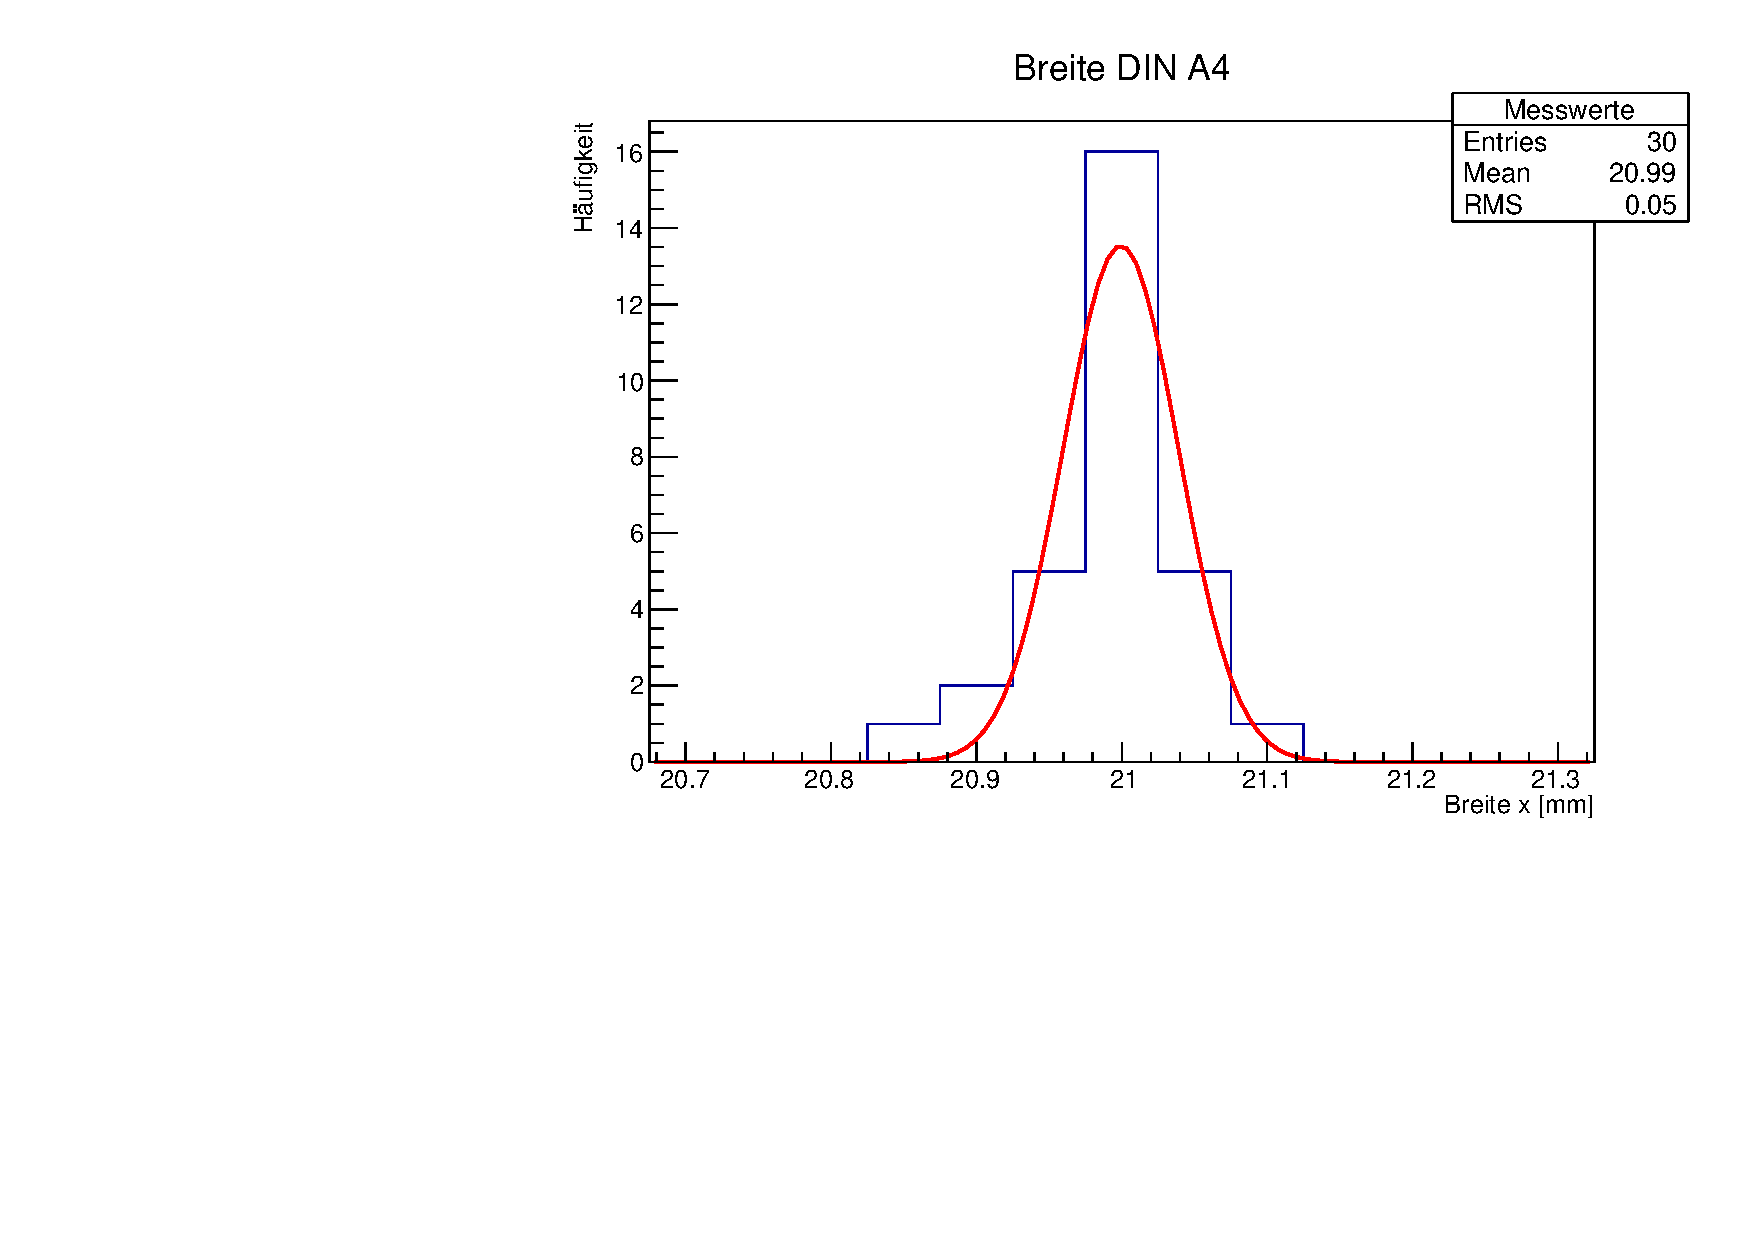
\includegraphics[width=1.00\textwidth]{00_einl/messung_histo.pdf}
	\captionof{figure}{Häufigkeitsverteilung der Messwerte aus Tabelle \ref{tab:MessungDINA4}}
	\label{fig:messung_histo}
\end{minipage}

Die Breite der Häufigkeitsverteilung wird durch die Standardabweichung $\sigma$ beschrieben, je größer diese ist, desto breiter ist die Kurve. Der Wendepunkt der Kurve befindet sich im Abstand $\sigma$ vom Mittelwert. Berechnet man die Fläche unter der Kurve zwischen den beiden Wendepunkten, so ergibt sich:
\begin{equation}
	\frac{1}{\sqrt{2\pi}\sigma}\int_{\bar{x}-\sigma}^{\bar{x}+\sigma}{e^{-\frac{\left(x-\bar{x}\right)^2}{2\sigma^2}}dx} = 0,683
\end{equation}

Das bedeutet, dass die Wahrscheinlichkeit, einen Messwert im Intervall $\left[\bar{x}-\sigma; \bar{x}+\sigma\right]$ zu finden (für $n\rightarrow\infty$), 68,3\% beträgt.

\noindent
Andere oft genutzte Intervalle sind:
\begin{align*}
	\mathrm{1-fache Standardabweichung} &\quad \phantom{0}\bar{x}-\sigma \; \mathrm{bis}\; \bar{x}+\sigma & (68,3\%)\\
	\mathrm{2-fache Standardabweichung} &\quad \bar{x}-2\sigma\; \mathrm{bis}\; \bar{x}+2\sigma & (95,5\%)\\
	\mathrm{3-fache Standardabweichung} &\quad \bar{x}-3\sigma\; \mathrm{bis}\; \bar{x}+3\sigma & (99,7\%)
\end{align*}
%**********************************************************************************************************************
\subsection{Die Unsicherheit eines Messergebnisses}

Da wir als Messergebnis den Mittelwert angeben, ist die Messunsicherheit definiert durch die Frage: \textit{Wie weit weicht der Mittelwert $\bar{x}$ aller Messungen vom wahren Wert $\mu$ ab?}

Diese Abweichung nimmt mit zunehmender Anzahl an Messungen immer weiter ab, der Mittelwert nähert sich dem wahren Wert immer mehr an. Bei einer großen Anzahl an Messungen gilt für die \textit{statistische Unsicherheit des Mittelwertes}:
\begin{important}
	\begin{equation}
		\Delta{\bar{x}} = \frac{\sigma_x}{\sqrt{n}}
	\end{equation}
\end{important}

Den Intervall $\left[\bar{x}-\Delta\bar{x}; \bar{x}+\Delta\bar{x}\right]$ nennt man den \textit{Konfidenzbereich auf dem Vertrauensniveau 68,3\%}. Die Aussage ''Der Messwert beträgt $\bar{x}\pm\Delta\bar{x}$'' bedeutet, dass wenn man den Messvorgang wiederholen würde (mit der gleichen Anzahl an Einzelmessungen $n$), für mindestens $68,3\%$ der auf Grundlage der Messdaten berechneten Konfidenzintervalle der wahre Wert im jeweiligen Konfidenzintervall liegt.

\paragraph{Bemerkung:} Korrektur für kleine Anzahl von Messungen

\begin{table}[t]	
	\centering
		\begin{tabular}[t]{|c|c|c|c|} 
			 & 68,3\% & 95\% & 99,7\% \\ 
			n & t & t & t \\\hline
			2 & 1,84 & 12,71 & 235,8 \\
			3 & 1,32 & 4,30 & 19,21 \\
			4 & 1,20 & 3,18 & 9,22 \\
			5 & 1,15 & 2,78 & 6,62 \\
			6 & 1,11 & 2,57 & 5,51 \\
			8 & 1,08 & 2,37 & 4,53 \\
			10 & 1,06 & 2,26 & 4,09 \\
			20 & 1,03 & 2,09 & 3,45 \\
			30 & 1,02 & 2,05 & 3,28 \\
			50 & 1,01 & 2,01 & 3,16 \\
			100 & 1,00 & 1,98 & 3,08 \\
			200 & 1,00 & 1,97 & 3,04 
		\end{tabular}
	\captionof{table}{Werte der Student-t-Verteilung für verschiedene Konfidenzintervalle}
	\label{tab:Student-t}
\end{table}

\noindent
Liegen nur wenige Messungen vor, so ist die Annahme nicht mehr wahr, dass die Verteilung der Messwerte durch die Normalverteilung beschrieben wird. Stattdessen muss die Student-t-Verteilung verwendet werden. Den Unterschied der beiden Verteilungen berücksichtigen wir durch einen Korrekturfaktor $t$, der Tabelle \ref{tab:Student-t} entnommen werden kann.

\noindent
Für die Unsicherheit des Messwertes gilt dann:
\begin{equation}
 \Delta \bar{x} = \frac{t}{\sqrt{n}}\sigma_x = t\cdot \sigma_{\bar{x}}
\end{equation}

Wie man sieht, geht der Korrekturfaktor für $n\rightarrow\infty$ gegen $t=1$, denn für große Anzahlen an Einzelmessungen nähert sich die Student-t-Verteilung der Normalverteilung an.

%**********************************************************************************************************************
\subsection{Der gewichtete Mittelwert und seine Unsicherheit}

Bei der Bildung des arithmetischen Mittelwertes geht man implizit davon aus, dass alle Messwerte, die in die Mittelung aufgenommen werden, dieselbe Unsicherheit haben. Dies muss nicht immer der Fall sein.\\

Beispiel: \textit{Aus irgendeinem Grund verwenden Sie zur Messung derselben Länge unterschiedliche Maßstäbe. Z. Bsp. benutzen Sie für einige Messungen ein Lineal mit einer Genauigkeit von 1~mm, für andere Messungen eine Schieblehre, die eine Auflösung von 0,1~mm hat.}\\

Um diese unterschiedlich genauen Messungen sinnvoll in einem Mittelwert zu kombinieren, benutzt man den \textit{gewichteten Mittelwert}:
\begin{important}
	\begin{equation}
		\bar{x} = \frac{\sum_{i=1}^n{w_i\cdot x_i}}{\sum_{i=1}^n{w_i}}
	\end{equation}
\end{important}
wobei die Wichtungsfaktoren $w_i$ die Kehrwerte der Abweichungsquadrate sind:
\begin{equation*}
	w_i = \frac{1}{\Delta x_i^2}
\end{equation*}
Auf diese Weise tragen Messwerte mit größerer Unsicherheit weniger stark zum Mittelwert bei. Die Unsicherheit des gewichteten Mittelwertes beträgt:
\begin{equation}
	\Delta\bar{x} = \frac{1}{\sum_{i=1}^n{w_i}}
\end{equation}
Sind alle Wichtungsfaktoren $w_i$ gleich, geht der gewichtete Mittelwert in den 'normalen` über, und dessen Abweichung sinkt wieder mit der Wurzel der Zahl der Werte.\\

Der gewichtete Mittelwert gilt strenggenommen nur für normalverteilte Größen. Er wird aber mangels Alternativen auch auf andere statistische oder systematische Abweichungen angewandt. Vor einer Anwendung ist aber zu prüfen, ob die unterschiedlichen Messungen mit dem zugehörigen Konfidenzbereich überlappen. Falls dies nicht der Fall ist, liegt eine zusätzliche, nicht erkannte Abweichung vor (z.B. grobe Fehler).\\

Beispiel:
\textit{Drei Praktikumsgruppen erhalten die Aufgabe, den Durchmesser einer Dose zu bestimmen. Die erste Gruppe erhält eine Schieblehre als Hilfsmittel, die zweite ein 30~cm langes Lineal mit Millimeterskala und die Studierenden der dritten Gruppe müssen mit bloßem Auge den Durchmesser abschätzen:}

\begin{tabular}{|l|l|l|l|} \hline
		& Gruppe 1: & Gruppe 2: & Gruppe 3:\\
		& Durchmesser [mm] & Durchmesser [mm] & Durchmesser [cm]\\ \hline
	Messung 1 & 100,3 & 102,5 & 8 \\
	Messung 2 & 100,2 & 105,0 & 9\\
	Messung 3 & 100,4 & 102,0 & 10 \\
	Messung 4 & 100,1 & 107,0 & 13 \\
	Messung 5 & 100,2 & 100,5 & 6 \\
	Messung 6 & 100,3 & 101,0 & 12 \\
	Messung 7 & 100,5 & 102,5 & 9\\
	Messung 8 & 100,0 & 103,0 & 11\\
	Messung 9 & 100,4 & 102,5 & 12\\
	Messung 10 & 100,3 & 103,5 & 8 \\ \hline
	Mittelwert & 100,270 & 102,95 & 9,8\\ \hline
	Std. abw. & 0,047 & 0,60 & 0,70\\ \hline
\end{tabular}

\textit{Der Mittelwert aus allen diesen Messungen für den Dosendurchmesser $d$ ergibt:}
\begin{align}
	\bar{d} & = \frac{\frac{100,27}{0,047^2}+\frac{102,95}{0,60^2}+\frac{98}{7^2}}{\frac{1}{0,047^2}+\frac{1}{0,60^2}+\frac{1}{7^2}}\;\mathrm{mm} = 100,286\;\mathrm{mm}\\
	\Delta\bar{d} & = \frac{1}{\sqrt{\frac{1}{0,047^2}+\frac{1}{0,60^2}+\frac{1}{7^2}}}\;\mathrm{mm} = 0,047\;\mathrm{mm}
\end{align}
\textit{Als Messwert für den Durchmesser ergibt sich also: $d = (100,286\pm 0,047)\;\mathrm{mm}$.}
%**************************************************************
% Hier noch was zu Geräten und Aufspüren systematischer Fehler?
%**************************************************************

%**********************************************************************************************************************
%**********************************************************************************************************************
\section{Indirekte Messung: Fehlerfortpflanzung}

Wenn sich die gesuchte Größe aus zwei oder mehr einzeln gemessenen Größen zusammensetzt, so nennt man die Bestimmung der zusammengesetzten Größe eine \textit{indirekte Messung}. Ein Beispiel dafür ist schon die einfache Bestimmung der Fläche eines DIN A4 Blattes, die wir uns früher schon angeschaut haben.

Wie wir wissen, sind die einzelnen, direkten Messungen mit Unsicherheiten behaftet. Wie können wir aus diesen die Ungenauigkeit der indirekten Messung der zusammengesetzten Größe berechnen?

%**********************************************************************************************************************
\subsection{Größtfehlerbetrachtung}

Die einfachste Möglichkeit, den Fehler abzuschätzen, ist die Annahme, dass die Unsicherheiten aller Einzelgrößen voll zur Gesamtunsicherheit beitragen und sich nicht untereinander beeinflussen (man sagt \textit{sie sind nicht korreliert}).

Rechnerisch wird das umgesetzt, indem man in die Formel zur Berechnung der gesuchten zusammengesetzten Größe die Einzelmessungen $x_i \pm \Delta x_i$ so einsetzt, dass das Ergebnis maximal wird. Anschließend wird der Vorgang so wiederholt, dass das Ergebnis minimal wird. Die Differenz der beiden Ergebnisse bezeichnet man als den \textit{Größtfehler}.\\

%\noindent
Dieses Verfahren berücksichtigt den statistischen Zusammenhang der einzelnen Beiträge nicht, daher liefert es im Allgemeinen zu große Werte für die Unsicherheit. Darüber hinaus können sich rechnerische Schwierigkeiten ergeben, wenn z. Bsp. die entsprechende Größe in einer Summe im Nenner und im Zähler der Formel vorkommt. In diesem Fall ist es schwierig herauszufinden, ob die positive oder die negative Abweichung den größten bzw. den kleinsten Wert ergibt. Dieses Verfahren ist daher nur für den Notfall geeignet, liefert jedoch oft eine brauchbare Abschätzung.

%**********************************************************************************************************************
\subsection{Gauß'sche Fehlerfortpflanzung}

Betrachten wir eine Größe $g$, die nicht direkt gemessen werden kann, sich aber aus mehreren direkt gemessenen Größen $x$, $y$, $z$,... berechnen läßt:
\begin{equation}
	g = g(x,y,z,...)
\end{equation}
Der Einfachheit halber wollen wir uns im Folgenden auf die drei Messgrößen $x$, $y$ und $z$ beschränken, die Rechnungen können jedoch prinzipiell mit beliebig vielen Messgrößen durchgeführt werden.

Wir gehen davon aus, dass die Messserien für die Größen $x$, $y$ und $z$ normalverteilt sind. Dann kann der Mittelwert $\bar{g}$ der gesuchten Größe bestimmt werden, indem man die Mittelwerte der Messgrößen in die Formel einsetzt:
\begin{important}
	\begin{equation}
		\bar{g} = g(\bar{x},\bar{y},\bar{z})
	\end{equation}
\end{important}

Wenn die Messgrößen $x$, $y$ und $z$ statistisch unabhängig voneinander sind, man sagt \textit{unkorreliert}, dann kann die gesamte Unsicherheit wie folgt berechnet werden:
\begin{important}
	\begin{equation}
		\Delta\bar{g} = \sqrt{\Delta\bar{x}^2 \cdot \left(\frac{\partial g}{\partial x} \right)^2_{\bar{x},\bar{y},\bar{z}} + \Delta\bar{y}^2 \cdot \left(\frac{\partial g}{\partial y} \right)^2_{\bar{x},\bar{y},\bar{z}} + \Delta\bar{z}^2 \cdot \left(\frac{\partial g}{\partial z} \right)^2_{\bar{x},\bar{y},\bar{z}}}
	\end{equation}
\end{important}

Diese Formel ist bekannt als die \textit{Gauß'sche Fehlerfortpflanzung}, wenn für die Unsicherheiten $\Delta\bar{x}$, $\Delta\bar{y}$, $\Delta\bar{z}$ die jeweilige Standardabweichung eingesetzt wird.

Die Ausdrücke $\partial g/\partial x$, $\partial g/\partial y$ und $\partial g/\partial z$ stehen dabei für die partiellen Ableitungen der Formel zur Berechnung von $g$ nach den Variablen $x$, $y$ und $z$.

\paragraph{Beispiel:} Messung der Dichte eines Quaders\\
\textit{
Die Dichte eines Quaders ergibt sich aus seiner Masse $m$ und seinem Volumen $V = x\cdot y\cdot z$, wenn $x$, $y$ und $z$ die Kantenlängen sind, nach der Formel
\begin{equation}
	\rho = \frac{m}{V} = \frac{m}{x\cdot y\cdot z}
	\label{eq:Dichte}
\end{equation}
Bei der Messung der Masse und der Kantenlängen findet man die Werte $\bar{m}\pm \sigma_m$, $\bar{x}\pm \sigma_x$, $\bar{y}\pm \sigma_y$ und $\bar{z}\pm \sigma_z$. Die partielle Ableitung von Gleichung \ref{eq:Dichte} nach der Masse $m$ ist:
\begin{equation*}
	\frac{\partial \rho}{\partial m} = \frac{1}{x\cdot y\cdot z}
\end{equation*}
Die partielle Ableitung nach $x$ lautet (für die anderen beiden Richtungen genauso vorgehen):
\begin{equation*}
	\frac{\partial \rho}{\partial x} = -\frac{1}{x}\cdot\frac{m}{x\cdot y\cdot z}
\end{equation*}
Damit ergibt sich für die Unsicherheit der Dichte:
\begin{equation}
	\Delta\bar{\rho} = \sqrt{\Delta\bar{x}^2\left(-\frac{1}{\bar{x}}\frac{m}{\bar{x}\bar{y}\bar{z}} \right)^2 + \Delta\bar{y}^2\left(-\frac{1}{\bar{y}}\frac{m}{\bar{x}\bar{y}\bar{z}} \right)^2 + \Delta\bar{z}^2\left(-\frac{1}{\bar{z}}\frac{m}{\bar{x}\bar{y}\bar{z}} \right)^2 + \Delta\bar{m}^2\left(\frac{1}{\bar{x}\bar{y}\bar{z}}\right)^2}
\end{equation}
In diese Gleichung sind jetzt nur noch die jeweiligen Mittelwerte und Unsicherheiten einzusetzen, um die Unsicherheit der Dichte zu berechnen.
}\\

Falls die einzelnen Messgrößen nicht normalverteilt sind, oder wenn sie nicht statistisch von einander unabhängig sind, muss man bei der Fortpflanzung der Unsicherheiten noch einen Korrekturfaktor berücksichtigen, der diese Korrelation der Messgrößen beschreibt. Diesen nennt man den \textit{Korrelationskoeffizienten}.

%**********************************************************************************************************************
\subsection{Fortpflanzung systematischer Abweichungen}

Systematische Abweichungen entziehen sich naturgemäß einer statistischen Behandlung. Man kann insbesondere nicht davon ausgehen, dass es unwahrscheinlich ist,
dass alle Abweichungen der Beteiligten Einzelgrößen gleichzeitig extremal sind.\\

Beispiel:
\textit{Eine Veränderung der Umgebungstemperatur bei der Messung zieht eine Abweichung aller Längenmessungen gemeinsam nach sich, da der Maßstab natürlich bei jeder Messung
'falsch' ist. Man muss also in diesem Fall davon ausgehen, dass die Abweichungen nicht quadratisch addiert werden dürfen, sondern linear addiert werden müssen. Der Einfluss jeder
Einzelabweichung muss voll auf die Gesamtabweichung durchschlagen.}\\

\textit{Im Fall einer systematischen Abweichung der Längenmessung durch einen nicht gleichmäßig geteilten Maßstab erscheint es jedoch sinnvoll anzunehmen, dass je nach Position die Abweichung unterschiedlich ist. Entsprechend kann man auch davon ausgehen, dass nicht gerade alle Abweichungen zum gleichen Zeitpunkt in die gleiche Richtung gehen. Hier ist also eine quadratische Addition sinnvoll.}\\

Es hängt also vom Einzelfall ab welche Methode der Fortpflanzung bei einer systematischen Abweichung angewandt werden muss. Die lineare Addition bei potentiell statistisch gekoppelten Vorgängen oder die quadratische Addition bei definitiv statistisch unabhängigen Vorgängen.\\
Sei beispielsweise die Größe $g$ aus drei Variablen $x, y, z$ zusammengesetzt, die jeweils die systematischen Unsicherheiten $\Delta x, \Delta y, \Delta z$ haben. Dann erfolgen lineare und quadratische Addition wie folgt:

\textbf{Lineare Addition}
\begin{equation} \label{eq:error_lin_add}
	\Delta\bar{g} = \left|\Delta\bar{x}\cdot \left[\frac{\partial g}{\partial x}\right]_{\bar{x}, \bar{y}, \bar{z}}\right|
								+ \left|\Delta\bar{y}\cdot \left[\frac{\partial g}{\partial y}\right]_{\bar{x}, \bar{y}, \bar{z}}\right|
								+ \left|\Delta\bar{z}\cdot \left[\frac{\partial g}{\partial z}\right]_{\bar{x}, \bar{y}, \bar{z}}\right|
\end{equation}

\textbf{Quadratische Addition}
\begin{equation} \label{eq:error_quad_add}
	\Delta\bar{g} = \sqrt{\Delta\bar{x}^2\cdot \left[\frac{\partial g}{\partial x}\right]^2_{\bar{x}, \bar{y}, \bar{z}}
											+ \Delta\bar{y}^2\cdot \left[\frac{\partial g}{\partial y}\right]^2_{\bar{x}, \bar{y}, \bar{z}}
											+ \Delta\bar{z}^2\cdot \left[\frac{\partial g}{\partial z}\right]^2_{\bar{x}, \bar{y}, \bar{z}}}
\end{equation}
%**********************************************************************************************************************
\subsection{Verknüpfung statistischer und systematischer Unsicherheiten}

Auch bei der Verknüpfung systematischer und statistischer Unsicherheiten ist die Frage nach de Kopplung der Gr"o{\ss}en zu beachten. Die Frage, ob die statistische Unsicherheit von der systematischen Abweichung abhängig ist oder nicht, ist jedoch letztlich nicht beantwortbar. Entsprechend werden in der Literatur auch beide Meinungen vertreten.\\

\noindent
\textbf{Im Praktikum} wollen wir vom konservativen Fall ausgehen und annehmen, dass die beiden Beitr"age nicht voneinander unabh"angig sind und befolgen die folgenden Schritte:
\begin{enumerate}
	\item Bestimmung der statistischen Unsicherheit aus allen Einzelgrößen mittels \textit{quadratischer Addition} nach Gleichung \ref{eq:error_quad_add}.
	\item Bestimmung der systematischen Unsicherheit aus \textit{linearer Addition} aller Einzelgrößen nach Gleichung \ref{eq:error_lin_add}.
	\item Verknüpfung der statistischen und systematischen Unsicherheit mittels normaler linearer Addition, nicht Gleichung \ref{eq:error_lin_add}, zur Gesamtunsicherheit, welche dann beim Ergebnis angegeben wird.
\end{enumerate}
%**********************************************************************************************************************
%\begin{todo}
	%Einen Abschnitt über systematische Unsicherheiten und wie man sie abschätzt.
%\end{todo}

%**********************************************************************************************************************
%**********************************************************************************************************************
%\section{Graphische Auswertung bei korrelierten Messwerten}
%
%Dein einfachste Beziehung zwischen zwei Messgrößen ist die \textit{lineare Abhängigkeit}
%\begin{equation}
	%y(x) = a\cdot x + b
%\end{equation}
%mit den beiden freien Parametern $a$ und $b$.
\chapter{Fehlerrechnung und Auswertungen im Praktikum} \label{v:fehler}

\section{Allgemeines}

Dieser Abschnitt m"usste eigentlich richtiger hei"sen: "`Rechnen mit
Ungenauigkeiten"'\index{Ungenauigkeiten}. Im Folgenden sollen kurz
einige Grundlagen zur Fehlerrechnung\index{Fehlerrechnung},
Statistik\index{Statistik} und Auswertung von
Messdaten\index{Auswertung} dargelegt werden, soweit sie f"ur
dieses Praktikum wichtig sind. F"ur eine genauere Betrachtung sei
auf die Spezialliteratur
%\cite{beving,bron,npp,kamke,physmess,lichten,tbstat,tbnum,taylor,messunsicher}
verwiesen.\\

\noindent
Dieser Abschnitt ist der Praktikumsanleitung für Physiker entnommen. Inhaltlich sollte er größtenteils mit dem vorherigen Abschnitt übereinstimmen, führt aber einige der Konzepte in größerer Tiefe ein.

\section{Vorbemerkung}

Eine physikalische Gr"o"se\index{Gr"o"se!Physikalische} kennzeichnet
Eigenschaften und beschreibt Zust"ande sowie Zustands"anderungen von
Objekten der Umwelt. Sie muss nach einer Forderung von
\person{Einstein} messbar sein. Die Vereinbarung, nach der die
beobachtete physikalische Einheit quantifiziert wird, ist die
Einheit der physikalischen Gr"o"se. Somit besteht eine physikalische
Gr"o"se {\bf G} immer aus einer quantitativen Aussage G (Zahlenwert)
und einer qualitativen Aussage [G] (Einheit): {\bf G} = G $\cdot$
[G].

F"ur physikalische Gr"o"sen gilt: "`Physikalische Gr"o"se = Zahlenwert
$\cdot$ Einheit"', also bitte immer Einheiten angeben.\footnote{Die
Betreuerinnen sollen Protokolle mit fehlenden Einheiten
zur"uckgeben.} Gesetzlich vorgeschrieben ist die Verwendung des
\emph{Internationalen Einheitensystems
(SI-Einheiten)}\index{SI-Einheiten}. Im amtlichen und gesch"aftlichen
Verkehr d"urfen nur noch SI-Einheiten\index{Einheit} benutzt werden. Teilweise muss man als Naturwissenschaftler aber
auch mit anderen, "alteren Einheiten umgehen k"onnen (Bsp.: Torr,
Gau"s). %Einen sehr sch"onen "Ubersichtsartikel "uber physikalische
%Gr"o"sen, deren Nomenklatur und Einheiten, finden Sie in Ref.~\cite{codata}.

Die Messung einer physikalischen Gr"o"se\index{Gr"o"se!physikalische}
erfolgt %durch Vergleich der Einheit dieser Gr"o"se nach der
Messmethode der (SI-)Vereinbarung oder einem darauf aufbauenden
Messverfahren. Je nach Genauigkeit des Messverfahrens tritt ein
unterschiedlich grosser Messfehler (Ungenauigkeit, Abweichung) auf.
Dabei ist zwischen den \emph{systematischen}, f"ur das Messverfahren
charakteristischen Messfehlern\index{Messfehler} und den
\emph{zuf"alligen} oder \emph{statistischen}, vom einzelnen
Experiment abh"angigen Fehlern zu unterscheiden. Zu systematischen
Messfehlern geh"oren z.B. eine falsche Kalibrierung eines
Messger"ates, Ablesefehler (Parallaxe), falsche Justierung,
Messwertdrift, etc. Zu statistischen Fehlern geh"oren (zuf"allige)
Schwankungen wie elektronische Triggerschwankungen,
Temperaturschwankunken, Rauschen, ungenaues Anlegen von Ma"sst"aben
etc. Zur grafischen Analyse der Messwertschwankungen dient das
Histogramm. Bei zuf"alligen Messfehlern ist die H"aufigkeitsverteilung
der Messwerte $N_j(x_j)$ symmetrisch zu einem Mittelwert, dem
Erwartungswert $\mu$. Wird die Anzahl $n$ der Wiederholungsmessungen
stark erh"oht, so geht die (diskrete) relative H"aufigkeitsverteilung
$N_j(x_j) \rightarrow h(x)$ in eine glockenf"ormige Normalverteilung
(\person{Gau"s}sche Verteilungsfunktion) mit der
Halbwertsbreite\index{Halbwertsbreite} $\Gamma$ (= halbe Breite der Kurve
in halber H"ohe des Maximums, engl.~\textsc{HWHM=Half Width at Half
Maximum}) der Messwerte "uber:
%
\begin{important}
\begin{equation}\label{e:gaussnormal}
    h(x) = \frac{1}{\sqrt{2 \pi}\sigma} e^{-\frac{(x-\mu)^2}{2 \sigma^2}}
    \qquad \mbox{mit} \qquad
    \sigma = \frac{\Gamma}{\sqrt{2 \, \ln 2}} \, .
\end{equation}
\end{important}

Der Parameter $\sigma$ ist ein Ma"s f"ur die Breite der
Verteilungsfunktion $h(x)$: 68,3~\% der Messwerte liegen im Bereich
$\mu - \sigma < x < \mu + \sigma $. Aus der H"aufigkeitsverteilung $h(x_j)$
einer endlichen Anzahl $N$ von Messungen der $m$ diskreten
Messwerte $x_1, \ldots x_m$ lassen sich f"ur 
$\mu$ und $\sigma$ nach der Theorie der
Beobachtungsfehler von \person{Gau"s} Sch"atzwerte berechnen.
Demnach ist die beste N"aherung f"ur $\mu$ der arithmetische
Mittelwert $\bar{x}$, f"ur $\sigma$ die
Standardabweichung $s$, die sich aus der
Fehlersumme berechnet (s.u.). 
%Letztere ist minimal, wenn der
%arithmetische Mittelwert als Erwartungswert gesetzt wird (siehe
%unten).

\section{Ungenauigkeiten und Fehler}

Alle Messvorg"ange liefern Messergebnisse mit einem Fehler, der
nach einer verbindlichen "Ubereinkunft ein Ma"s f"ur die Genauigkeit
des Messergebnisses darstellt. Ein Beispiel: Die L"ange eines
Stabes wird durch Anlegen eines Ma"sstabes bestimmt. Dann sind zwei
Arten von Fehlern m"oglich:
%
\begin{enumerate}
  \item der systematische Fehler des Ma"sstabs, der sich durch genauen Vergleich
   mit dem Urmeter\index{Urmeter} ermitteln l"asst,
  \item der zuf"allige Fehler, der sich durch Unsicherheiten beim Anlegen des
 Ma"sstabs ergibt.
\end{enumerate}

Alle Messergebnisse m"ussen deshalb mit Fehlerangabe $\bar{x} \pm
\Delta x$ angeben werden. In den meisten
F"allen darf man annehmen, dass die Messwerte um den wahren Wert
statistisch streuen, d.h. dass die Abweichungen im Betrag
schwanken und im Mittel gleich oft positiv wie negativ
ausschlagen. Dann ist der beste Wert (Bestwert)\index{Bestwert},
den man aufgrund von $n$ wiederholten Messungen mit Messergebnis
$x_i$ angeben kann, der Mittelwert\index{Mittelwert} $\bar{x}$:
%
\begin{important}
\begin{equation}\label{e:mw}
\mbox{Mittelwert: } \,  \bar{x} = \frac{1}{n} \sum_{i=1}^n x_i \,
.
\end{equation}
\end{important}
%
Au"ser den Streufehlern, die man auch zuf"allige - oder statistische
- Fehler nennt, treten gew"ohnlich auch so genannte systematische
Fehler auf. Ist ein Messger"at falsch kalibriert, wird es zum
Beispiel immer zu gro"se Werte liefern. Um eine Aussage "uber die
Zuverl"assigkeit des Messergebnisses machen zu k"onnen, muss die
Gr"o"se dieser beiden Fehlereinfl"usse abgesch"atzt werden. Die
Aufgabe der Fehlerrechnung ist also die Bestimmung des Fehlers
$\Delta x = \Delta x_{\rm syst.} + \Delta x_{\rm stat.}$. Das Ergebnis der
Messung mit Fehlerangabe\index{Fehlerangabe} lautet dann:
%
\begin{equation}\label{e:ergfehler}
  \mbox{Ergebnis mit Fehlerangabe: } \,  \bar{x} \pm \Delta x \, .
\end{equation}
%
Diese Angabe bedeutet: Man erwartet, dass der wahre Wert $x_w$ im
Bereich $\bar{x} - \Delta x \leq x_w \leq \bar{x} + \Delta x $
liegt. $\Delta x$ nennt man den absoluten Fehler. Es kann auch der
relative Fehler angegeben werden: $\Delta x / \bar{x}$.

Da jede gemessene physikalische Gr"o"se mit einem Fehler behaftet ist,
macht es keinen Sinn als Ergebnis eine Zahl mit vielen Ziffern
anzugeben. Die Zahl der angegebenen Ziffern sollte an die Gr"o"se des
Fehlers angeglichen werden, d.h. das Ergebnis ist entsprechend
sinnvoll zu runden. Das Ergebnis und der Fehler werden an der
gleichen Stelle gerundet. Der Fehler wird normal gerundet.


\section{Systematische Fehler}

Systematische Fehler\index{Fehler!systematische} bei Messungen im
Praktikum r"uhren haupts"achlich von Ungenauigkeiten der Messger"ate
oder der Messverfahren her. Abweichungen der Messbedingungen, wie
z.B. der Temperatur, spielen in der Regel eine untergeordnete
Rolle. Beispiele f"ur systematische Fehler sind:
%
\begin{itemize}
  \item Eine Stoppuhr geht stets vor oder nach
  \item Ein Voltmeter zeigt wegen eines Kalibrierfehlers einen stets zu gro"sen
   (oder zu kleinen) Wert an
  \item Der Ohmsche Widerstand in einer Schaltung weicht vom
  angegebenen Nominalwert ab.
  \item Eine Beeinflussung der Messung durch Messger"ate (z.B.
  Innenwiderst"ande) wird nicht ber"ucksichtigt.
\end{itemize}
%
Systematische Fehler haben stets einen festen Betrag und ein
eindeutiges Vorzeichen. Sie "andern sich auch nicht, wenn die Messung
mit der gleichen Anordnung und den gleichen Ger"aten wiederholt wird.
Da das Vorzeichen nicht bekannt ist, muss man sie auch mit dem
unbestimmten Vorzeichen $\pm$ angeben. F"ur die Absch"atzung des
Betrages gelten die folgenden Hinweise.

F"ur Messger"ate sind die maximal erlaubten Abweichungen $\Delta
x_{\rm syst.}$ einer Anzeige $x$ vom wahren Wert in der Regel durch
Herstellungsnormen festgelegt (G"ute des Ger"ates, siehe
Beschreibung bei "`Messger"aten"'). F"ur elektrische Messger"ate ist
der Begriff "`G"uteklasse"' eingef"uhrt worden. Diese gibt den
erlaubten systematischen Fehler als Prozentwert vom Vollausschlag
an. Diesen Fehler setzt man dann f"ur alle Messungen in diesem
Messbereich an.

Bei L"angenmessger"aten betr"agt der m"ogliche systematische Fehler
selten mehr als wenige Promille vom Messwert und kann daher
gegen"uber den Streufehlern in den meisten F"allen vernachl"assigt
werden. F"ur eine quantitative Absch"atzung kann die folgende Formel
verwendet werden:
%
\begin{equation}\label{e:skalafehler}
  \frac{\Delta x_{\rm syst}}{x} =
  \frac{\mbox{1 Skalenteil der Skala}}{\mbox{Skalenteile bei Vollausschlag.}}
\end{equation}

Stoppuhren sind noch genauer und Ihr Fehler kann zu $\Delta
x_{\rm syst} = \mbox{kleinster Skalenwert} + {\rm 0.005} \cdot
\mbox{Messwert} $ abgesch"atzt werden.

Bei der Messung von Temperaturen mit einem Fl"ussigkeitsthermometer
betr"agt der Ger"atefehler etwa 1~Strichabstand.


\section{Statistische, zuf"allige Fehler}

Ursachen f"ur zuf"allige Fehler\index{Fehler!statistische} sind z.B.
Schwankungen der Messbedingungen w"ahrend der Messung oder auch
Ungenauigkeiten bei der Ablesung von Messinstrumenten (z.B.
Parallaxe). Um den Betrag des Streufehlers absch"atzen zu k"onnen,
wiederholt man die Messung mehrfach. Ein Ma"s f"ur die Streuung kann
dann aus den Abweichungen $x_i - \bar{x}$ der einzelnen Messwerte
vom Mittelwert gewonnen werden, die von Gau"s als
Standardabweichung $s$ f"ur $n$ Messungen $x_i$ definiert wurde:
%
\begin{equation}\label{e:standabw}
  s = \sqrt{ \frac{1}{n-1} \sum_{i=1}^n \left( x_i - \bar{x} \right)^2 }
\end{equation}

Die Standardabweichung $s$ repr"asentiert die Genauigkeit der
einzelnen Messung und damit auch des Messverfahrens. Deshalb wird
$s$ auch als mittlerer quadratischer Fehler der Einzelmessung
bezeichnet. Je mehr Einzelmessungen vorliegen, umso genauer wird
der Mittelwert sein. Der mittlere quadratische Fehler des
Mittelwertes $\Delta x_{\rm stat.}$ ist nach der Fehlertheorie um den
Faktor $\nicefrac{1}{\sqrt{n}}$ kleiner.
%
\begin{important}
\begin{equation}\label{e:fmw}
 \Delta x_{\rm stat} = \frac{s}{\sqrt{n}}
     = \sqrt{ \frac{1}{n(n-1)} \sum_{i=1}^n \left( x_i - \bar{x} \right)^2 }
\end{equation}
\end{important}
%
Dieser Wert $\Delta x_{\rm stat}$ wird manchmal in Anlehnung an
die Normalverteilung als $\sigma_{\bar{x}}$ bezeichnet. 
Dabei sollte der Wert $\sigma_{\bar{x}}$, der den Fehler auf
den arithmetischen Mittelwert $\bar{x}$ angibt, {\it nicht} mit dem
Fehler $\sigma=s$ der Einzelmessung $x_i$ verwechselt werden!
Die Fehlerrechnung
erlaubt dann die Aussage (wenn systematische Fehler wesentlich
kleiner sind), dass der wahre Wert mit einer Wahrscheinlichkeit
von 68\% im Intervall mit der Breite $\sigma_{\bar{x}}$ um den Mittelwert
liegt: $\bar{x} - \sigma_{\bar{x}} < x_w < \bar{x} + \sigma_{\bar{x}} $.

%Nach der Theorie der Beobachtungsfehler (t-Verteilung nach
%Student, alias \person{W. S. Gosset}) sind bei normalverteilten
%Messgr"ossen die Vertrauensgrenzen abh"angig von der Anzahl $n$ der
%Messungen und der Standardabweichung $s$ des Messverfahrens:
%
%\begin{equation}\label{e:t-vert}
%    x = \bar{x} \pm t_P \cdot \frac{s}{\sqrt{n}}
%\end{equation}
%
%Der Faktor $t_P$ folgt aus der Student-t-Verteilung und ist
%abh"angig von der Anzahl der Wiederholungsmessungen und der
%geforderten statistischen Sicherheit $P$
%\cite{bron,tbstat}. F"ur gro"se $n$ entspricht
%$t_{\numprint[\%]{68.3}}$=1. %, d.h. $\Delta x = \Delta \bar{x}$.
%Einige Werte f"ur $t_P$ sind in Tabelle~\ref{t:student} aufgef"uhrt.

Im Praktikum, wie meistens in der
Physik, k"onnen wir uns mit 1$\sigma$, also 68,3~\% Sicherheit zufrieden geben.
Bitte geben Sie Ihre Ergebnisse in den Protokollen auch so an,
d.h. benutzen Sie die $1\sigma$"=Regel f"ur Ihre Fehlerangaben.
Liegt neben der statistischen Unsicherheit auch noch ein
systematischer Fehler vor, so ist als Gesamt-Messfehler die quadratische Summe
der beiden Fehler anzugeben.
%
%\begin{table}[htb]%
%  \centering%
%  \caption[Student-Verteilung: Werte von $t_P$]{\label{t:student}Einige Werte
%  von $t_P$ bei der Student"=t"=Verteilung
%   f"ur die angegebene statistische Sicherheit.}%
%  \begin{tabular}{rrrr}%
%    \toprule
%    $n$ & 68.3\% & 95\% & 99.7\% \\ \midrule
%    3   & 1.32 & 4.3 & 19.2 \\
%    5   & 1.15 & 2.8 & 6.6\\
%    10  & 1.06 & 2.3 & 4.1\\
%    100 & 1.00 & 2.0 & 3.1\\ \bottomrule
%  \end{tabular}
%\end{table}


\section{Gewichteter Mittelwert}

Bei Vorliegen mehrerer \emph{unabh"angiger} Ergebnisse ist es "ublich,
den gewichteten Mittelwert\index{Mittelwert!gewichtet} anzugeben:
%
\begin{important}
\begin{equation}\label{e:gewmittel1}
 \bar x = \frac{
   \sum\limits_i \frac{x_i}{\sigma_i^2 }
    }{
    \sum\limits_i \frac{1}{\sigma_i^2}
    }
    \quad \mbox{mit Fehler: } \quad
    \sigma  = \sqrt{\frac{1}{\sum\limits_i \frac{1}{\sigma_i^2}} } \, .
\end{equation}
\end{important}
%
Bei stark unterschiedlich genauen Werten greift man besser auf
folgende Berechnung des Fehlers zur"uck:
%
\begin{equation}\label{e:gewsigma2}
 \sigma  = \sqrt {\frac{{\sum {\frac{{\left( {x_i  - \bar x}
 \right)^2 }}{{\sigma _i^2 }}} }}{{\left( {n - 1} \right)\sum
 {\frac{1}{{\sigma _i^2 }}} }}} \, ,
\end{equation}
%
oder nimmt das Maximum des mit den beiden obigen Formeln
berechneten Fehlers.

\section{Lineare Regression}

Hat man die Messwerte $y_i(x_i)$ vorliegen und vermutet einen
linearen Zusammenhang $y=m\cdot x + b$, so kann man dies einfach
mit der linearen Regression\index{Lineare Regression} testen. 

\subsection{Einfache Regression}

Ohne Ber"ucksichtigung bzw.~Kenntnis der Fehler auf die Messwerte 
$y_i$ ergibt sich f"ur die Steigung aus der linearen Regression:
%
\begin{equation}
m = \frac{{n\sum {x_i y_i  - \sum {x_i \sum {y_i } } } }}{{n\sum
{x_i^2  - \left( {\sum {x_i } } \right)^2 } }}
\end{equation}
%
und der Achsenabschnitt ist
%
\begin{equation}
b = \frac{{\sum {x_i^2 \sum {y_i }  - \sum {x_i \sum {x_i y_i } }
} }}{{n\sum {x_i^2  - \left( {\sum {x_i } } \right)^2 } }}
\end{equation}
%
Die jeweiligen Fehler berechnen sich zu:
%
\begin{equation}
\sigma_m^2  = \frac{{n\sum {\left( {y_i  - b - mx_i } \right)^2 }
}}{{\left( {n - 2} \right)\left( {n\sum {x_i^2  - \left( {\sum
{x_i } } \right)^2 } } \right)}}
\end{equation}
%
\begin{equation}
\sigma_b^2  = \frac{{\sum {x_i^2  \cdot } \sum {\left( {y_i  - b -
mx_i } \right)^2 } }}{{\left( {n - 2} \right)\left( {n\sum {x_i^2
- \left( {\sum {x_i } } \right)^2 } } \right)}}
\end{equation}
%
und der Korrelationskoeffizient\index{Korrelationskoeffizient}
berechnet sich folgenderma"sen:
%
\begin{equation}
 r = \frac{
 {n\sum {x_i y_i  - \sum {x_i \sum {y_i } } } }
 }
 {
 {\sqrt{n\sum {x_i^2  - \left( {\sum {x_i } } \right)^2 }} \cdot
  \sqrt{n\sum {y_i^2  - \left( {\sum {y_i } } \right)^2 } } }
 }
\end{equation}
%
Mathematisch liefert der Korrelationskoeffizient ein Ma{\ss} daf"ur, ob die Annahme eines linearen Zusammenhangs zwischen den $x_i$ und $y_i$ sinnvoll ist. Je dichter der Betrag des Korrelationskoeffizienten bei Eins liegt, desto besser ist die Linearit"at.\\
Man sei aber vorsichtig, aus einem guten $r$ sofort auf einen
wirklich physikalischen linearen Zusammenhang zu schlie"sen.

\subsection{Regression mit Messfehlern} \label{v:LinRegErr}

Unter der Voraussetzung, dass nur die
$y_i$-Werte mit dem Fehler $\sigma_i$ fehlerbehaftet, w"ahrend die
$x_i$-Werte fehlerfrei sind, ergibt sich f"ur die lineare Regression:
\begin{align*}
\Delta&=\sum{\frac{1}{\sigma_i^2}}\sum{\frac{x_i^2}{\sigma_i^2}}-
\left(\sum{\frac{x_i}{\sigma_i^2}}\right)^2 & &
\\
%
m&=\frac{1}{\Delta}\left(\sum{\frac{1}{\sigma_i^2}}
\sum{\frac{x_iy_i}{\sigma_i^2}}-\sum{\frac{x_i}{\sigma_i^2}}\sum{\frac{y_i}{\sigma_i^2}}
\right)
&\sigma_m&=\sqrt{\frac{1}{\Delta}\sum{\frac{1}{\sigma_i^2}}} \\
%
b&=\frac{1}{\Delta}\left(\sum{\frac{x_i^2}{\sigma_i^2}}
\sum{\frac{y_i}{\sigma_i^2}}-\sum{\frac{x_i}{\sigma_i^2}}\sum{\frac{x_iy_i}{\sigma_i^2}}
\right) \hspace{11mm}
&\sigma_b&=\sqrt{\frac{1}{\Delta}\sum{\frac{x_i^2}{\sigma_i^2}}} \\
%
\chi^2&=\sum{\left[\frac{1}{\sigma_i}\left(y_i-mx_i-b\right)\right]^2} & &
\end{align*}


\section{Mathematische Behandlung}

\subsection{Grundlagen der Fehlerrechnung: Bestwert und Fehler}

Wir betrachten im Folgenden einen vorher berechneten Mittelwert
aus Messergebnissen f"ur eine physikalische Gr"o"se und bezeichnen
diesen mit $M$. F"ur diese Gr"o"se $M$ kennen wir den wahren Wert
$M_W$, der in einem wirklichen Experiment nat"urlich unbekannt ist,
aber als existent angenommen werden kann. Jeder Messwert $M_i$ der
Gr"o"se $M$ weicht vom wahren Wert um den absoluten Fehler $\Delta M_i$
ab:
%
\begin{equation} \label{b}
 \Delta M_i = M_i - M_W \, .
\end{equation}
%
Das Endergebnis einer $n$-mal wiederholten Bestimmung von $M$ soll
durch einen Bestwert $M_B$ beschrieben werden, der der Vorschrift
%
\begin{equation} \label{c}
\sum_{i=1}^{n}\, (M_{i} - M_{B})^{2} = f(M_{B}) = \mbox{Minimum}
\end{equation}
%
gen"ugt, die als \person{Gau"s}sche Methode der kleinsten
(Fehler-)Quadrate zur Bestimmung des Bestwertes\index{Bestwert}
bezeichnet wird. F"uhrt man die Bestimmung des Minimums nach der
Vorschrift
%
\begin{equation} \label{d}
 \frac{d}{d M_B} \sum_{i=1}^{n}(M_{i} - M_{B})^{2} = 0
\end{equation}
%
aus, so ergibt sich
%
\begin{equation} \label{e}
 M_{B} = \frac{1}{n} \sum_{i=1}^{n} M_{i} = \bar M
\end{equation}
%
und damit die Definition:
%
\begin{definition} \label{def:bestwert}
  Der Bestwert ist gleich dem arithmetischen Mittel.
\end{definition}

Der in (\ref{b}) definierte absolute Fehler der
Einzelmessung\index{Fehler!der Einzelmessung} l"asst sich in der
Praxis nicht ermitteln. Deshalb f"uhren wir nach der Vorschrift
%
\begin{equation} \label{f}
 \Delta M = \sqrt{
  \frac{1}{n-1} \sum_{i=1}^{n} \left( M_{i} - M_{B} \right)^{2}
 }
\end{equation}
%
den mittleren quadratischen Fehler der Einzelmessung ein. Der in
(\ref{f}) eigentlich erwartete Gewichtsfaktor $1/n$ wurde durch
$1/(n-1)$ ersetzt, weil man f"ur 1~Messwert nat"urlich keinen Fehler
berechnen kann.


\subsection{Die Normalverteilung}

Normalerweise sind die Messdaten $M_i$ gen"ahert in Form einer
Glockenkurve um den wahren Wert $M_W$, angen"ahert durch den
Bestwert $M_B$, verteilt. Die mathematische Form der
Glockenkurve\index{Glockenkurve} ist gegeben durch die
\person{Gau"s}sche
Normalverteilung\index{Normalverteilung}\index{Gau"s}:
%
\begin{important}
\begin{equation} \label{g}
  P(x) =
  \frac{1}{\sqrt{2\pi} \sigma} \cdot
  \exp\left( -\frac{(x-\bar{x})^{2}}{2\sigma^{2}} \right)
\end{equation}
\end{important}
%
wobei $x = M_i - M_B$ gesetzt wurde und somit hier $\bar{x}=0$
gilt. Dar"uber hinaus wird die Normierung erf"ullt:
%
\begin{equation} \label{h}
  \int_{-\infty}^{+\infty}\,P(x) dx = 1 \, .
\end{equation}
%
Eine solche \emph{Glockenkurve} ist in Bild~\ref{a:glockenkurve}
schematisch dargestellt.
%
\begin{figure}[htb]
  \centering
% \setcapindent{1em}
% \begin{captionbeside}
  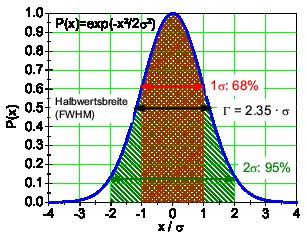
\includegraphics[width=8cm]{00_einl/gaussfkt}
% \end{captionbeside}
 \caption[Gau"ssche Glockenkurve]{\label{a:glockenkurve}Schematische Darstellung
   der Glockenkurve. Die Abzisse ist in Vielfachen von $\sigma$ angegeben.
   Auf die Normierung
   der Ordinate wurde der "Ubersicht wegen verzichtet. Die schraffierten
   Intervalle geben die jeweiligen Sicherheitsintervalle von 68.3~\%
   ($1\sigma$) und 95~\% ($2\sigma$) wieder (siehe Text).}
\end{figure}
%
Weiter kann folgende Formel hergeleitet werden:
%
\begin{equation} \label{i}
 s^2 = \int_{-\infty}^{+\infty}\,P(x) \cdot (x-\bar{x})^{2} dx = \sigma^{2}
\end{equation}
%
Das bedeutet, dass der Parameter $\sigma$ der Glockenkurve mit deren 
Standardabweichung $s$ "ubereinstimmt. Man kann
ferner zeigen, dass die Wahrscheinlichkeit, den wahren Wert
innerhalb des $1\sigma$"=Intervalls um $\bar{x}$ zu finden

\begin{equation} \label{j}
  W(\sigma) = \int_{\bar{x}-\sigma}^{\bar{x}+\sigma} \, P(x) dx =
  0.68
\end{equation}
%
betr"agt. Beziehung (\ref{j}) beinhaltet, dass die Angabe des
mittleren quadratischen Fehlers nicht bedeutet, dass f"ur alle
Messwerte $M_i$ die Abweichung vom Bestwert $M_B$ kleiner als
$\sigma$ ist. Vielmehr betr"agt die relative H"aufigkeit
(Wahrscheinlichkeit oder Sicherheit) hierf"ur nur 68\%.


\subsection{Der Bestwert einer Funktion und Fehlerfortpflanzung}

Der Bestwert einer Funktion $f(x,y,...)$ von verschiedenen
unabh"angigen Messgr"o"sen $x,y,...$ erschwert die Fehlerrechnung
etwas, und es muss das
Fehlerfortpflanzungsgesetz\index{Fehlerfortpflanzungsgesetz}
angewandt werden. Gegeben seien die Messwerte
%
\begin{equation} \label{l}
  x_{i},\quad i=1\ldots r; \hspace{2cm} y_{k},\quad k=1\ldots s \,
  ,
\end{equation}
%
aus denen ein Endergebnis $f_{i,k}=f(x_{i},y_{k})$ berechnet wird.
Beispiel: Berechnung der Fl"ache $A$ eines Rechtecks aus den
Kantenl"angen $x$ und $y$. Es l"asst sich zeigen, dass der Bestwert
$\bar A$ von $A$ gegeben ist durch
%
\begin{equation} \label{m}
 \bar f \equiv  \frac{1}{r} \cdot \frac{1}{s} \cdot
  \sum_{i=1}^{r} \sum_{k=1}^{s} f(x_{i},y_{k}) = f(\bar x, \bar y)
  \, .
\end{equation}
%
Dieses Ergebnis gilt f"ur beliebige Funktionen und beliebig viele
Variablen. Wir bezeichnen jetzt die mittleren quadratischen Fehler
von $f$, $x$ und $y$ mit $\sigma_f$, $\sigma_x$ bzw. $\sigma_y$.
Dann l"asst sich unter Benutzung der Definitionen der mittleren
quadratischen Fehler dieser drei Gr"o"sen zeigen, dass ein
Fehlerfortpflanzungsgesetz\index{Fehlerfortpflanzung} in der Form
%
\begin{equation} \label{n}
 \sigma_{f} =
   \sqrt{\sigma_{x}^{2} \left( \frac{\partial f}{\partial x} \right)^{2}
    +
         \sigma_{y}^{2} \left( \frac{\partial f}{\partial y} \right)^{2}
   }
\end{equation}
%
gilt\footnote{Die gilt, wie eingangs angenommen, {\it nur} f"ur unab"angige
Messgr"o"sen. Andernfalls muss ein zus"atzlicher Term, der die Korrelation
zwischen $x$ und $y$ ber"ucksichtig, hinzugef"ugt werden.}. 
Auch in (\ref{n}) sind beliebig viele Variablen zugelassen.
Spezialf"alle von (\ref{n}) sind:
%
\begin{equation} \label{o}
  \bar f = \bar x + \bar y \qquad \mbox{mit: } \qquad
  \sigma_{f} = \sqrt{\sigma_{x}^{2} + \sigma_{y}^{2}}
\end{equation}
%
\begin{equation} \label{q}
  \bar f = \bar x \cdot \bar y \qquad \mbox{mit: } \qquad
  \frac{\sigma_{f}}{\bar f}  = \sqrt{\left(\frac{\sigma_{x}}{\bar
 x}\right)^{2} + \left(\frac{\sigma_{y}}{\bar y}\right)^{2}} \, .
\end{equation}
%
%


\subsection{Der mittlere quadratische Fehler des Bestwertes}

Die Beziehung (\ref{f}) gibt den mittleren quadratischen Fehler
$\Delta M_{i}$ der Einzelmessung $M_{i}$ an.\footnote{Hier werden
h"aufig auch die Begriffe "`Standardabweichung"' $s$ oder
"`Varianz"' $s^2$ verwendet. Die Verwendung der Begriffe erfolgt
nicht immer einheitlich, man sollte daher auf die jeweilige
Definition achten.} Da aber nicht die Einzelmessung sondern der
Bestwert $M_B$ das Endergebnis darstellt, muss der Fehler des
Bestwertes\index{Fehler!des Mittelwertes} $\Delta M_{B}$ bestimmt
werden. Dazu fassen wir $M_B$ als Funktion der Gr"o"sen $M_{i}$ auf,
d.h.:
%
\begin{equation} \label{s}
M_{B} = \frac{1}{n} \sum_{i=1}^{n}\,M_{i} = f(M_{1}, M_{2},...)
\end{equation}
%
und wenden hierauf das Fehlerfortpflanzungsgesetz
%
\begin{equation} \label{t}
 \Delta M_{B} = \sqrt{\sum_{i=1}^{n}\,\left(\sigma_{i}\,\frac{\partial
 f}{\partial M_{i}}\right)^{2}}
\end{equation}
%
an. Da alle $\sigma_i$ als gleich angenommen werden k"onnen , d.h.
$\sigma_i$ =$\sigma$, und
%
\begin{equation} \label{u}
 \frac{\partial f}{\partial M_{i}} = \frac{1}{n}
\end{equation}
%
ist, ergibt sich schlie"slich:
%
\begin{important}
\begin{equation} \label{v}
 \Delta M_{B} = \frac{\sigma}{\sqrt{n}}  =
  \sqrt{\frac{1}{n(n-1)} \sum_{i=1}^{n} (\Delta M_{i})^{2}} \, .
\end{equation}
\end{important}
%
Genau dies sollte auch in den Protokollen zur Fehlerangabe
verwendet werden.




\subsection{Methode der kleinsten Fehlerquadrate (Minimales $\chi^2$)}

Ein h"aufig vorkommendes Problem ist die Anpassung einer glatten
Kurve an eine Folge von Messpunkten, die zur Bestimmung der
Kurvenparameter dienen sollen. Die Anpassung von Funktionen an
Messwerte erfolgt meist nach der Methode der kleinsten Quadrate
(minimales $\chi^2$). Als Beispiel benutzen wir das radioaktive
Zerfallsgesetz:
%
\begin{equation} \label{w}
  N(t)\,=\,N_{0} \exp(-\lambda t) \, ,
\end{equation}
%
welches die Anzahl $N(t)$ der nicht zerfallenen
radioaktiven Kerne als Funktion der Zeit $t$ beschreibt. In
(\ref{w}) ist $N_0$ die Zahl der Kerne zum Zeitpunkt $t=0$ und
$\lambda$ die Zerfallskonstante, die "uber die Beziehung
%
\begin{equation} \label{x}
  \lambda = \frac{\ln 2}{T_{1/2}}
\end{equation}
%
mit der Halbwertszeit $T_{1/2}$ des radioaktiven Materials
(Nuklids) zusammenh"angt. Zur Vereinfachung setzen wir voraus, dass
$N_0$ aus anderen Messungen bekannt ist, so dass nur noch
$T_{1/2}$ zu bestimmen ist. Wir messen $n$ mal die pro Zeiteinheit
stattfindenen Zerf"alle (Aktivit"at) und stellen uns die Aufgabe,
$T_{1/2}$ durch geeignete Anpassung der Funktion~(\ref{w}) an die
Messwerte zu bestimmen. Die Messung liefert
%
\begin{equation} \label{y}
 \mbox{Wertepaare} (N_i, t_i) \, ,
\end{equation}
%
d.h. die zum Zeitpunkt $t_i$ pro Zeiteinheit gemessene Anzahl
$N_i$ radioaktiver Kerne. Die Vorschrift f"ur die Anpassung der
Funktion (\ref{w}) lautet:
%
\begin{equation} \label{z}
  \chi^{2}(T_{1/2}) =
    \sum_{i=1}^{n} \frac{(N_{i}-N(t_{i}))^{2}}{\sigma_{i}^{2}} = \mbox{Minimum} \, .
\end{equation}
%
In (\ref{z}) bedeutet $\sigma_i$ den mittleren quadratischen
Fehler von $N_i$, der nach den Gesetzen der Statistik f"ur
diskrete, z"ahlbare Ereignisse
(Poisson-Statistik\index{Poisson-Statistik}) durch die Beziehung
%
\begin{equation} \label{aa}
  \sigma_i^2 = N_i
\end{equation}
%
gegeben ist. Wir vergleichen in (\ref{z}) also die Abweichung jedes
Messwertes $N_i$ von der gew"ahlten Kurve mit dem Fehler des
Messwertes und minimieren die Summe der mit dem reziproken Fehler
gewichteten Abweichungsquadrate\index{Abweichungsquadrate}.
Ausdr"ucke der Form (\ref{z}) werden allgemein mit $\chi^2$
bezeichnet und beinhalten die Gau"ssche Methode der kleinsten
Quadrate. Die praktische Auswertung der Vorschrift (\ref{z})
erfolgt, indem man $\chi^2$ f"ur eine Anzahl geeignet erscheinender
Werte $T_{1/2}$ berechnet und das Minimum mit Hilfe einer grafischen
Darstellung der Funktion $\chi^2$($T_{1/2}$) bestimmt.
%%%%%%%%%%%%%%%%%%%%%%%%%%%%%%%%%%%%%%%%%%%%%%%%%%%%%%%%%%%%%%%%%%%

\chapter {Erstellung von Diagrammen} \label{v:diagramme}

Hier folgen einige kurze Hinweise zur Erstellung von Diagrammen in
den Protokollen des Praktikums.

\section{Allgemeines}

Die meisten Auswertungen in der Physik werden heute mit sehr
umfangreichen Programmpaketen durchgef"uhrt, die auch gleichzeitig
eine komfortable Diagrammerstellung erlauben. Dennoch kann es
vorkommen, dass man eine einfache Auswertung sehr viel schneller
und mit guter Genauigkeit auch auf konventionellem Wege auf
Millimeterpapier oder Logarithmenpapier ausf"uhren kann. Zudem sind
die hier folgenden Hinweise auch sehr n"utzlich, wenn man
Computerprogramme zur Diagrammerstellung verwendet.

Manuelle Diagramme sind grunds"atzlich immer auf Millimeter- oder
Logarithmenpapier anzufertigen. Bei Computerprogrammen kann auf dies
verzichtet werden, dennoch sollte man auch hier auf eine leichte
Ablesbarkeit der Daten achten.

\section{Achsen}


\begin{enumerate}
    \item Wahl der Achsen: Die unabh"angige (die eingestellte)
    Variable sollte auf der waagerechten Achse, der "`x-Achse"'
    (Abszisse\index{Abszisse}), aufgetragen werden. Die abh"angige (die
    gemessene) Variable sollte auf der vertikalen Achse, der "`y-Achse"'
    (Ordinate\index{Ordinate}), aufgetragen werden.
    \item Achseneinteilung: Die Achseneinteilung sollte so gew"ahlt
    werden, das die Werte eines Datenpunktes einfach und schnell
    ermittelt werden k"onnen. Drei Einheiten einer Gr"o{\ss}e auf einem Zentimeter einzuzeichnen macht also nicht viel Sinn.
    \item Nullpunktsunterdr"uckung: Der Wertebereich der Achsen
    sollte so gew"ahlt werden, dass ein m"oglichst gro"ser Bereich
    ausgef"ullt wird (mindestens 75\% des Diagrammbereiches). Hierbei kann der Nullpunkt
    unterdr"uckt werden, wenn kein triftiger Grund dagegen
    spricht. Das bedeutet, dass die Einheiten auf Abszisse und Ordinate nicht unbedingt bei x=y=0 anfangen m"ussen. Dies gilt auch f"ur logarithmische Skalen.
    \item Achsen sind zu beschriften! Was ist aufgetragen?
    Zahlenwerte sind anzugeben. Einheiten sind unverzichtbar.
    \item Bei logarithmierten Werten ist die Angabe der Einheit problematisch,
     da der Logarithmus im Argument keine Einheit haben darf. Hier teilt man die
     Messwerte einfach durch die Einheit und erh"alt so reine Zahlenwert. Dies ist
     dann auch so anzugeben.
\end{enumerate}

\section{Datenpunkte und Fehlerbalken}

\begin{itemize}
    \item Symbole: Die Messpunkte sollten durch deutliche Symbole
    gekennzeichnet werden. "Ublich sind zum Beispiel: $ \square \blacksquare
    \blacktriangle \blacktriangledown \lozenge \blacklozenge \vartriangle
    \triangledown \bullet \bigcirc \circ \ast \star$.
    \item Unterschiedliche Messreihen sollten auch durch
    unterschiedliche Symbole gekennzeichnet werden. Auf eine
    eindeutige Legende ist zu achten. Farbe kann hier sehr
    n"utzlich sein, doch diese geht leider beim Kopieren verloren.
    \item Fehlerbalken: Normalerweise sind alle Messpunkte mit
    Fehlerbalken zu versehen, deren L"ange der Gr"o"se des (1$\sigma$-)Fehlers
    auf den jeweiligen Messwert entspricht. Dabei kann es notwendig sein, in
    den verschiedenen Achsrichtungen unterschiedlich gro"se
    Fehlerbalken zu verwenden.
\end{itemize}

\section{Kurven und Verbindungslinien}


\begin{itemize}
    \item Eine durchgezogene Kurve kann die Lesbarkeit einer
    Darstellung deutlich erh"ohen. Dennoch sollte dies mit Bedacht
    angewendet werden.
    \item In allen F"allen des Praktikums sind "`glatte"' Kurven zu
    erwarten. Zumeist ist der funktionale Zusammenhang der
    Messdaten auch durch die Theorie schon bekannt. Im Allgemeinen
    sollte eine Kurve m"oglichst wenig Wendepunkte haben.
    \item Es ist nicht zwingend erforderlich, dass die
    durchgezogene Kurve alle, oder "uberhaupt, Messpunkte trifft.
    Endpunkte sind meist weniger genau und m"ussen nicht unbedingt
    getroffen werden. Das einfache lineare Verbinden der
    Messpunkte durch eine
    "`Zick-Zack-Kurve"' ist physikalisch kompletter Unsinn und
    sollte unterlassen werden.
    \item Die Kurve sollte m"oglichst dicht an den Messpunkten
    liegen (Minimierung der Fehlerquadrate). Die eingezeichneten
    Fehlerbalken k"onnen hier eine gute Hilfe sein. Zudem ist das
    Auge ein sehr guter "`Computer"' f"ur die Ausgleichskurve.
    \item Im Wesentlichen sollte die Kurve die Messpunkte
    halbieren, d.h. eine H"alfte der Punkte "uber der Kurve, die
    andere darunter. Das gilt sinngem"a"s auch f"ur Teilst"ucke.
    \item An Regressionsgeraden sind auch die Ergebnisse der
    Regression mit den richtigen Einheiten anzugeben.
    \item Bei Ermittlung des Fehlers "uber Grenzgeraden, sind auch
    diese in der Zeichnung anzudeuten.
\end{itemize}

Als Beispiel f"ur die Diagrammerstellung sind in
Bild~\ref{a:graph_beisp} zwei typische Diagramme aufgef"uhrt.
%
\begin{figure}[htb]
  \centering
  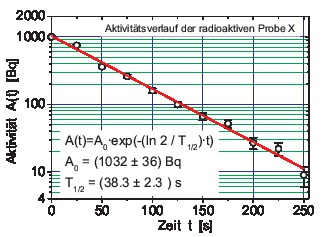
\includegraphics[width=6.5cm]{00_einl/graph_expzerf}
  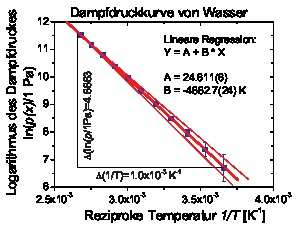
\includegraphics[width=6.5cm]{00_einl/graph_dampf}
  \caption[Diagramm-Beispiele]{\label{a:graph_beisp}Beispiele f"ur grafische Auftragungen
   zu Messwerten und Auswertungen:
  a) (links) Halblogarithmische Darstellung des exponentiellen Zerfalls;
  b) (rechts) Arrheniusplot der Dampfdruckkurve von Wasser. }
\end{figure}
%
Die Aktivit"atskurve wird
halblogarithmisch\index{Logarithmenpapier!halblogarithmisch}
aufgetragen, d.h. die Zeit normal (linear) als x-Achse, w"ahrend
die Aktivit"at logarithmisch
(Logarithmenpapier\index{Logarithmenpapier}) aufgetragen
wird.\footnote{Es erfolgt keine Umrechnung der Messwerte, die
Skalenteilung ist logarithmisch, genauer gesagt
halblogarithmisch.} Dies hat zur Folge, dass aus der
Exponentialfunktion eine lineare Funktion wird:
%
\begin{equation}\label{e:bsp_exp}
    A(t)=A_0 \cdot \exp(-\lambda t) \Longrightarrow \ln(A(t)) =
    \ln(A_0) - \lambda t
\end{equation}
%
Die Zerfallskonstante $\lambda$ kann dann aus der Steigung $m$ der
sich ergebenden Geraden ermittelt werden, woraus dann die
Halbwertszeit folgt. Man beachte die unterschiedliche L"ange der
Fehlerbalken. F"ur viele Skalengesetze und stark streuende Messwerte,
oder wenn man den Zusammenhang nicht genau kennt, verwendet man die
doppeltlogarithmische
Auftragung\index{Logarithmenpapier!doppeltlogarithmisch}, die f"ur
fast alle beliebigen Messungen eine Gerade entstehen l"asst.

In Bild~\ref{a:graph_beisp}b) ist ein Arrheniusplot des Dampfdruckes
von Wasser aufgetragen. Hier werden die Messwerte (in Pa) vor dem
Auftragen durch ihren Logarithmus ersetzt. Da das Argument des
Logarithmus keine Einheit enthalten kann, behilft man sich, indem
man durch die Einheit dividiert (d.h. diese "`Basiseinheit"' muss
auch im Diagramm mit angegeben werden). Durch die Auftragung der
logarithmierten Messwerte gegen die reziproke Temperatur erh"alt man
eine Gerade
%
\begin{equation}\label{e:bsp_dampf}
    p(T) = p_0 \cdot \exp\left( - \frac{\Lambda}{RT} \right) \Rightarrow
    \ln\left( p(T) \right) = \ln(p_0) - \frac{\Lambda}{R} \cdot
    \frac{1}{T} \, ,
\end{equation}
%
aus deren Steigung die Verdampfungsenthalpie $\Lambda$ berechnet
werden kann. Das Steigungsdreieck ist eingezeichnet und die Steigung
ergibt sich zu
$m=\frac{\mathrm{4.883}}{\mathrm{1\cdot 10^{-3}\, K^{-1}}}=\mathrm{4883~K}$.\footnote{Bitte
beachten Sie, dass die Steigung nat"urlich eine Einheit hat, die
angegeben werden muss.} Mit der allgemeinen Gaskonstanten
$R=\mathrm{8.3145\,J \, mol^{-1} \, K^{-1}}$ ergibt sich die
Verdampfungsw"arme zu $\Lambda=m \cdot R = \mathrm{40597\,J \,mol^{-1}}$ mit einem Fehler von $\Delta \Lambda = \mathrm{20\,J \,mol^{-1}}$.

%
%%%%%%%%%%%%%%%%%%%%%%%%%%%%%%%%%%%%%%%%%%%%%%%%%%%%%%%%%%%%%%%%%%%%
\cleardoublepage
\part{Versuche}


\renewcommand{\thechapter}{\arabic{chapter}}
\setcounter{chapter}{0}
\def\chaptername{Versuch}
\setcounter{tocdepth}{0}
%
%%%%%%% Vorf�hrversuch %%%%%%%
\documentclass[11pt, twoside, a4paper]{book}

\usepackage{graphicx}
\usepackage[utf8]{inputenc}
\usepackage{ngerman}
%\usepackage{lineno}
\usepackage{verbatim}
\usepackage[squaren]{SIunits}
\usepackage{amsmath}
\usepackage{amsfonts}
\usepackage{amssymb}
\usepackage{enumitem}
\usepackage{fancyhdr}
\usepackage{textcomp}
\usepackage{subcaption}
\usepackage[noadjust]{marginnote}
\usepackage{tikz}
\usepackage{nicefrac}
\usepackage{framed}

\usetikzlibrary{calc,intersections}
\usetikzlibrary{arrows}
\usetikzlibrary{decorations.markings}
\usetikzlibrary{decorations.pathreplacing}
\usepackage[european resistors]{circuitikz}
\usepackage[ 
    top=2cm, 
    bottom=2cm, 
    outer=3cm, 
    inner=3cm,
    marginparwidth=2.5cm,
		headheight=14pt
  ]{geometry}

\usepackage{parskip}
\usepackage{pdfpages}

\setlength{\parindent}{0pt}

\newcommand{\experimentheader}[4]
{
  \iftutor{{\bf Schwierigkeitsgrad:} #1\\}
  \iftutor{{\bf Dauer:} #2\\}
  {\bf Ger\"ate:} #3\\
  {\bf Bauteile:} #4
}

\newcommand{\hintboxNone}{0}
\newcommand{\hintboxExclamation}{1}
\newenvironment{hintbox}[4][\hsize]
{
  \def\FrameCommand
  {%
    {\color{#3}\vrule width 3pt}%
    \hspace{0pt}%must no space.
    \fboxsep=\FrameSep\colorbox{#4}%
  }%
  \MakeFramed{\hsize#1\advance\hsize-\width\FrameRestore}%
  \mbox{\textbf{#2}:}%
}
{
  \endMakeFramed
}
\newcommand{\xhintbox}[3]
{
  \begin{hintbox}{Achtung}{red!50}{red!10}
    #3
  \end{hintbox}
}

\newenvironment{hint}
{
  \begin{hintbox}{Hinweis}{green!50}{green!10}
}
{
  \end{hintbox}
}

\newenvironment{definition}
{
  \begin{hintbox}{Definition\\}{white!50}{white!10}
}
{
  \end{hintbox}
}

\newenvironment{important}
{
  \begin{hintbox}{Hinweis}{gray!50}{gray!10}
}
{
  \end{hintbox}
}

\newenvironment{jason}
{
  \begin{hintbox}{Achtung}{red!50}{red!10}
}
{
  \end{hintbox}
}

\newcommand{\mandatoryenumi}
{
  \renewcommand{\labelenumi}{\arabic{enumi}.} 
}
\newcommand{\optionalenumi}
{
  \renewcommand{\labelenumi}{$\bigstar$\quad\arabic{enumi}.} 
}
\newcommand{\mandatoryenumii}
{
  \renewcommand{\labelenumii}{(\alph{enumii})} 
}
\newcommand{\optionalenumii}
{
  \renewcommand{\labelenumii}{$\bigstar$\quad(\alph{enumii})} 
}
\newcommand{\icname}[1]{\mbox{\tt #1}}


  %\newcommand{\iftutor}[1]{}
\newcommand{\ifnotutor}[1]{#1}

  \newcommand{\iftutor}[1]{#1}
\newcommand{\ifnotutor}[1]{}


\newenvironment{tutorhint}{\comment}{\endcomment}
\newenvironment{todo}{\comment}{\endcomment}
\newenvironment{solution}{\comment}{\endcomment}
\iftutor
{
  \renewenvironment{todo}
  {
    \hintbox{Todo}{red!50!yellow!90}{red!50!yellow!20}
  }
  {
    \endhintbox
  }
  \renewenvironment{tutorhint}
  {
    \hintbox{Tutorenhinweis der Stunde}{blue!50}{blue!10}
  }
  {
    \endhintbox
  }
  \renewenvironment{solution}
  {
    \hintbox{L\"osung}{black!80}{black!5}
  }
  {
    \endhintbox
  }
}
\newcommand{\etutorhint}[1]
{
  \iftutor{
    \tutorhint
      #1
    \endtutorhint
  }
}
\newcommand{\esolution}[1]
{
  \iftutor
  {
    \solution
    #1
    \endsolution
  }
}
\newcommand{\etodo}[1]
{
  \iftutor
  {
    \todo
    #1
    \endtodo
  }
}



\begin{document}

\renewcommand{\thechapter}{\arabic{chapter}}
\setcounter{chapter}{0}
\def\chaptername{Versuch}

\chapter*{Vorversuch: Federpendel}
\label{v:0}

\etodo{\textbf{Prakikumsleitung:} Am Tag vor dem ersten Vorführversuch zusammen mit Hörsaal Vorbereitung aufbauen.}
In diesem Versuch, der vor Beginn des Praktikums im Rahmen einer Einführungsveranstaltung zusammen mit der Praktikumsleitung und den Tutoren durchgeführt wird, wollen wir Ihnen einige der wichtigsten Aspekte zur Durchführung der Praktikumsversuche, der Auswertung der Messdaten, sowie zur Protokollierung des Versuchs aufzeigen.
%------------------------------------------------
\section{Stichworte}
%------------------------------------------------

Federkonstante, Hookesches Gesetz, rücktreibende Kraft, Schwingung
%
%------------------------------------------------
\section{Literatur}
%------------------------------------------------

Gehrtsen, Kapitel 2.3
%
%------------------------------------------------
%\section{Anwendungsbeispiele}
%------------------------------------------------

%------------------------------------------------
\section{Theoretischer Hintergrund}
%------------------------------------------------

\subsection{Das Federpendel}

Das idealisierte Federpendel besteht aus einer Masse $m$, die an einer Schraubenfeder vernachlässigbarer Masse mit der Federkonstanten $D$ aufgehängt ist. Durch Vergrößern der Masse $m$ dehnt sich die Feder um einen Betrag $X=x-x_0$ gemäß dem Hookeschen Gesetz, d.h. die rücktreibende Kraft ist der Auslenkung proportional. Im Gleichgewichtsfall ist die Summe der Kräfte gleich Null:

\begin{equation} \label{eq:Federkonstante}
	m\cdot g - D\cdot X = 0 \quad \mathrm{mit\, g=9,81\,\frac{m}{s^2}}
\end{equation}

Lenkt man die Masse $m$ an der Feder aus und lässt sie zurückschnellen, bewirkt die rücktreibende Kraft $D\cdot X$ eine Beschleunigung $d^2X/dt^2$ in Richtung $x_0$. Damit lautet die Bewegungsgleichung:

\begin{equation}
	m\frac{d^2X}{dt^2} + D\,X = 0 \,.
\end{equation}

Das ist die Bewegungsgleichung einer harmonischen Schwingung, welche durch den Ansatz
\begin{equation}
	X(t) = X_a \cos(\omega t)
\end{equation}
gelöst wird. Darin ist $X_a$ die Amplitude (i.e. die maximale Auslenkung) und $\omega = \sqrt{\frac{D}{m}}$ die Kreisfrequenz der Schwingung. Die Periodendauer der Schwingung ist damit:
\begin{equation}
	T = \frac{2\pi}{\omega} = 2\pi\sqrt{\frac{m}{D}}
\end{equation}

Berücksichtigt man die homogen verteilte Masse der Feder, die sich bei der Schwingung mitbewegt, so erhält man einen korrigierten Ausdruck für die Schwingungsdauer:
\begin{equation} \label{eq:Schwingungsdauer}
	T_F = 2\pi\sqrt{\frac{m+\frac{m_F}{3}}{D}} \, ,
\end{equation}
wobei $m_F$ die Masse der Feder ist. Der Ausdruck $m+\frac{m_F}{3}$ stellt die \textit{effektive Masse} von Feder und Zusatzgewicht dar.
%------------------------------------------------
\section{Fragen zur Vorbereitung}
%------------------------------------------------

\begin{enumerate} 
	\item Welche Größen beschreiben eine Schwingung?
	%
	\item Weshalb schwingt ein Federpendel?
	%
  \item Wie lautet das Gravitationsgesetz?
	%
\end{enumerate} 

%------------------------------------------------
\section{Durchführung} 
%------------------------------------------------

\begin{enumerate}
	\item Messen Sie die Federkonstante $D$ mittels der \textit{statischen Methode}:
		\begin{enumerate}
			\item Messen Sie die Ausdehnung $x_0$ der Feder ohne angehängtes Gewicht. Wiederholen Sie die Messung drei Mal. Wie groß ist die Ablesegenauigkeit für diese Messung?
			%
			\item Messen Sie nun die Ausdehnung $x$ der Feder für verschiedene angehängte Gewichte: 50~g, 100~g, 150~g, 200~g. Wiederholen Sie die Messung jeweils drei Mal.
		\end{enumerate}
	%
	\item Messen Sie die Federkonstante nun \textit{dynamisch}:
		\begin{enumerate}
			\item Messen Sie die Masse $m_F$ der Feder.
			%
			\item Messen sie die Periodendauer für fünf Schwingungen der Feder bei angehängten Gewichten 50~g, 100~g, 150~g, 200~g. Wiederholen Sie die Messung jeweils drei Mal. Wie groß ist die Unsicherheit der Zeitmessung?
		\end{enumerate}
\end{enumerate}

%------------------------------------------------
\section{Auswertung} 
%------------------------------------------------

\begin{enumerate}
	\item Statische Methode:
		\begin{enumerate}
			\item Tragen Sie die mittlere Auslenkung $X = x_0 - x$ der Feder gegen das angehängte Gewicht auf. Dieses kann dabei als fehlerfrei angenommen werden.
			%
			\item Laut Gleichung \ref{eq:Federkonstante} gibt die Steigung dieser Gerade die Federkonstante $D$ an. Bestimmen Sie die Steigung der Geraden inklusive ihrer Unsicherheit.
		\end{enumerate}
	%
	\item Dynamische Methode:
		\begin{enumerate}
			\item Laut Gleichung \ref{eq:Schwingungsdauer} ist das Quadrat der Schwingungsdauer proportional zur Federkonstanten $D$. Tragen Sie daher den Mittelwert von $T^2$ gegen die effektive Masse auf.
			%
			\item Bestimmen Sie die Steigung der Geraden inklusive ihrer Unsicherheit und berechnen Sie daraus die Federkonstante $D$.
		\end{enumerate}
	%
	\item Vergleichen Sie die mit den beiden Methoden gemessenen Federkonstanten. Diskutieren Sie mögliche Abweichungen.
\end{enumerate}


\end{document}
%%%%%%%%%%%%%%%%%%%%%%%%%%%%%%
%
\documentclass[11pt, twoside, a4paper]{book}

\usepackage{graphicx}
\usepackage[utf8]{inputenc}
\usepackage{ngerman}
%\usepackage{lineno}
\usepackage{verbatim}
\usepackage[squaren]{SIunits}
\usepackage{amsmath}
\usepackage{amsfonts}
\usepackage{amssymb}
\usepackage{enumitem}
\usepackage{fancyhdr}
\usepackage{textcomp}
\usepackage{subcaption}
\usepackage[noadjust]{marginnote}
\usepackage{tikz}
\usepackage{nicefrac}
\usepackage{framed}
\usepackage{import}

\usetikzlibrary{calc,intersections}
\usetikzlibrary{arrows}
\usetikzlibrary{decorations.markings}
\usetikzlibrary{decorations.pathreplacing}
\usepackage[european resistors]{circuitikz}
\usepackage[ 
    top=2cm, 
    bottom=2cm, 
    outer=3cm, 
    inner=3cm,
    marginparwidth=2.5cm,
		headheight=14pt
  ]{geometry}

\usepackage{parskip}
\usepackage{pdfpages}

 \newcommand{\Ohm}{$\mathrm\Omega$}

\setlength{\parindent}{0pt}

\newcommand{\experimentheader}[4]
{
  \iftutor{{\bf Schwierigkeitsgrad:} #1\\}
  \iftutor{{\bf Dauer:} #2\\}
  {\bf Ger\"ate:} #3\\
  {\bf Bauteile:} #4
}

\newcommand{\hintboxNone}{0}
\newcommand{\hintboxExclamation}{1}
\newenvironment{hintbox}[4][\hsize]
{
  \def\FrameCommand
  {%
    {\color{#3}\vrule width 3pt}%
    \hspace{0pt}%must no space.
    \fboxsep=\FrameSep\colorbox{#4}%
  }%
  \MakeFramed{\hsize#1\advance\hsize-\width\FrameRestore}%
  \mbox{\textbf{#2}:}%
}
{
  \endMakeFramed
}
\newcommand{\xhintbox}[3]
{
  \begin{hintbox}{Achtung}{red!50}{red!10}
    #3
  \end{hintbox}
}

\newenvironment{hint}
{
  \begin{hintbox}{Hinweis}{green!50}{green!10}
}
{
  \end{hintbox}
}

\newenvironment{definition}
{
  \begin{hintbox}{Definition\\}{white!50}{white!10}
}
{
  \end{hintbox}
}

\newenvironment{important}
{
  \begin{hintbox}{Hinweis}{gray!50}{gray!10}
}
{
  \end{hintbox}
}

\newenvironment{jason}
{
  \begin{hintbox}{Achtung}{red!50}{red!10}
}
{
  \end{hintbox}
}

\newcommand{\mandatoryenumi}
{
  \renewcommand{\labelenumi}{\arabic{enumi}.} 
}
\newcommand{\optionalenumi}
{
  \renewcommand{\labelenumi}{$\bigstar$\quad\arabic{enumi}.} 
}
\newcommand{\mandatoryenumii}
{
  \renewcommand{\labelenumii}{(\alph{enumii})} 
}
\newcommand{\optionalenumii}
{
  \renewcommand{\labelenumii}{$\bigstar$\quad(\alph{enumii})} 
}
\newcommand{\icname}[1]{\mbox{\tt #1}}


  %\newcommand{\iftutor}[1]{}
\newcommand{\ifnotutor}[1]{#1}

  \newcommand{\iftutor}[1]{#1}
\newcommand{\ifnotutor}[1]{}


\newenvironment{tutorhint}{\comment}{\endcomment}
\newenvironment{todo}{\comment}{\endcomment}
\newenvironment{solution}{\comment}{\endcomment}
\iftutor
{
  \renewenvironment{todo}
  {
    \hintbox{Todo}{red!50!yellow!90}{red!50!yellow!20}
  }
  {
    \endhintbox
  }
  \renewenvironment{tutorhint}
  {
    \hintbox{Tutorenhinweis der Stunde}{blue!50}{blue!10}
  }
  {
    \endhintbox
  }
  \renewenvironment{solution}
  {
    \hintbox{L\"osung}{black!80}{black!5}
  }
  {
    \endhintbox
  }
}
\newcommand{\etutorhint}[1]
{
  \iftutor{
    \tutorhint
      #1
    \endtutorhint
  }
}
\newcommand{\esolution}[1]
{
  \iftutor
  {
    \solution
    #1
    \endsolution
  }
}
\newcommand{\etodo}[1]
{
  \iftutor
  {
    \todo
    #1
    \endtodo
  }
}



\begin{document}

\renewcommand{\thechapter}{\arabic{chapter}}
\setcounter{chapter}{16}
\def\chaptername{Versuch}

\chapter{Solarzelle und Halbleiterdiode}
\label{v:17}

Anhand der Charakteristiken von Halbleiterdioden und Solarzellen soll diese weit verbreitete Technologie näher gebracht werden.

%------------------------------------------------
\section{Stichworte}
%------------------------------------------------

Halbleiterdiode; Kennlinie einer Diode; Kennlinie einer Solarzelle (SZ), Arbeitspunkt (MPP) der SZ, Spektrale Empfindlichkeit der SZ; Farbe von Licht.
%
%------------------------------------------------
\section{Literatur}
%------------------------------------------------

Gehrtsen, Kapitel 11.1.2, 11.2.10, 11.3 und 14.4.3
%
%------------------------------------------------
\section{Anwendungsbeispiele}
%------------------------------------------------

Die Sonne ist die Hauptenergiequelle für unser tägliches Leben. Dabei kann diese Energie vor sehr langer Zeit geliefert worden sein, wie bei den fossilen Brennstoffen, indirekt, wie bei Windkraftwerken oder direkt, wie bei Sonnenkollektoren und Solarzellen. Solarzellen sind in Reihe geschaltete photoempfindlichen Halbleiterdioden, die zur Stromerzeugung genutzt werden. Die Spannung entsteht dabei durch optische Anregung von Valenzelektronen in das Leitungsband. Die mögliche Leistung, die eine Solarzelle zu erbringen vermag hängt dabei von der Beleuchtungsstärke und Farbe des beleuchtenden Lichtes ab. Im Versuch werden die physikalischen und elektrischen Eigenschaften von Halbleiterdioden studiert und die Energieerzeugung mit Hilfe einer Solarzelle quantitativ untersucht.

%------------------------------------------------
\section{Theoretischer Hintergrund}
%------------------------------------------------

\subsection{Halbleiter}

Durch die Anordnung im Kristallgitter verschieben sich die Energieniveaus der Siliziumatome ein klein wenig gegeneinander. Das führt dazu, daß die Niveaus in sogenannten Bändern nahe beieinanderliegen. Dasjenige Band, in dem sich die am schwächsten gebundenen Elektronen (Valenzelektronen) befinden, nennt man das \textit{Valenzband}. \\
Dieses ist durch eine \textit{Bandlücke}, in der es keine erlaubten Energieniveaus gibt, vom nächsthöheren Band getrennt. Da unter normalen Bedingungen keine Elektronen Zustände in diesem Band besetzen und die Energieniveaus benachbarter Atome energetisch sehr dicht aneinander liegen, kann ein Elektron, welches durch äußere Anregung in dieses Band gelangt, sich quasi-frei durch den Kristall bewegen und damit zur elektrischen Leitung beitragen. Daher bezeichnet man dieses Band als \textit{Leitungsband}.

\subsubsection{Dotierung}

Man kann in einen reinen Kristall aus vierwertigem Silizium bei der Herstellung Fremdatome einbringen, um die elektrische Charakteristik des Materials zu verändern. Dieser Prozess heißt \textit{Dotierung}.\\
Bringt man dreiwertige Atome in den Kristall (\textit{Akzeptor}, typischerweise Bor), so bleibt eine der Kristallbindungen zu den vier Nachbaratomen unvollständig, da ein Elektron für die kovalente Bindung fehlt. Diese unvollständige Bindung absorbiert leicht Elektronen aus dem Leitungsband, was ein fehlendes Elektron an einer anderen Stelle hinterläßt, da der Kristall insgesamt elektrisch neutral ist. Da auch diese neue, unvollständige Bindung leicht ein Elektron absorbiert, kann man dieses ''fehlende'' Elektron im Kristall als beweglich ansehen, es verhält sich also wie eine freie, positive Ladung. Man bezeichnet diese als \textit{Loch} im Valenzband. Auf diese Weise reichert eine Bor-Dotierung den Halbleiter mit positiven Ladungsträgern an, man nennt den Kristall auch \textit{p-dotiert}.\\
Auf dieselbe Weise führt Dotierung mit einem fünfwertigen Element (\textit{Donator}, typischerweise Phosphor) zu einem Überschuß an negativen Ladungsträgern, der Kristall ist \textit{n-dotiert}.

\subsection{$pn$-Diode}

Beim idealen $pn$-\"Ubergang grenzen zwei gleichm\"assig dotierte $p$-
und $n$-dotierte Schichten aneinander. Durch die unterschiedliche
Konzentration freier Ladungstr\"ager auf beiden Seiten kommt es zur
Diffusion: Elektronen des $n$-dotierten Gebiets wandern zur
$p$-dortierten Seite und k\"onnen dort mit L\"ochern rekombinieren. Die 
ortsfesten Atome, die ja nun ionisiert sind, stellen eine
positive {\it Raumladung} dar. Analog wandern L\"ocher aus der
$p$- in die $n$-Zone und rekombinieren. Eine negative Raumladung
entsteht.\\
Diese Raumladungen erzeugen ein elektrisches Feld,
welches der Diffusion entgegenwirkt und zu einem Gleichgewicht
f\"uhrt. Die Spannung, welche durch das elektrische Feld erzeugt
wird, nennt man {\it Diffusionsspannung}, $U_{\mathrm{D}}$. Das Gebiet
um den $pn$-\"Ubergang, welches frei von beweglichen Ladungstr{\"a}gern
 ist, wird {\it Verarmungszone} genannt. 
Die Ausdehnung der Verarmungszone auf die
jeweilige Seite ist proportional zum inversen der
Ladungstr\"agerkonzentration.

\subsubsection{$pn$-\"Ubergang mit \"ausserer Spannung in Durchlaßrichtung}

Legt man an den $pn$-\"Ubergang eine externe Spannung an, so dass die
Anode an die $p$-Schicht und die Kathode an die $n$-Schicht
angeschlossen ist, werden die Elektronen aus dem $n$-Gebiet zum
$p$-Gebiet hin verschoben und andersherum. Die angelegte Spannung,
$U_{\mathrm{F}}$, wirkt der Diffusionsspannung entgegen. Es gilt f\"ur
die Potentialdifferenz am $pn$-\"Ubergang:
%
\begin{equation}
U_{pn} = U_{\mathrm{Diff}} - U_{\mathrm{F}} \, .
\end{equation}

\noindent
Wenn die angelegt Spannung größer wird als die Diffusionsspannung, dann kann durch die Diode Strom fließen. Die Spannung, bei der das passiert nennt man \textit{Diodenspannung} $U_{\mathrm{D}}$ oder auch \textit{Vorwärtsspannung}. Mit zunehmender externer Spannung w\"achst der Strom durch den
$pn$-\"Ubergang. Man spricht von einem {\it Durchlassstrom}.

\subsubsection{$pn$-\"Ubergang mit \"ausserer Spannung in Sperrrichtung}

Legt man eine externe Spannung mit umgekehrter Polung,
$U_{\mathrm{R}}$, an den $pn$-\"Ubergang, so verst\"arkt diese die
Diffusionsspannung und man erh\"alt
%
\begin{equation}
U_{pn} = U_{\mathrm{Diff}} + U_{\mathrm{R}} \, .
\end{equation}

Die Elektronen der $n$-Schicht und die L\"ocher der $p$-Schicht werden
von der Verarmungszone weggezogen. Die Verarmungszone w\"achst. Da
kein Strom fließen kann wird diese Art der Beschaltung auch {\it
Sperrrichtung} genannt.

\begin{figure}[ht!]
\begin{center}
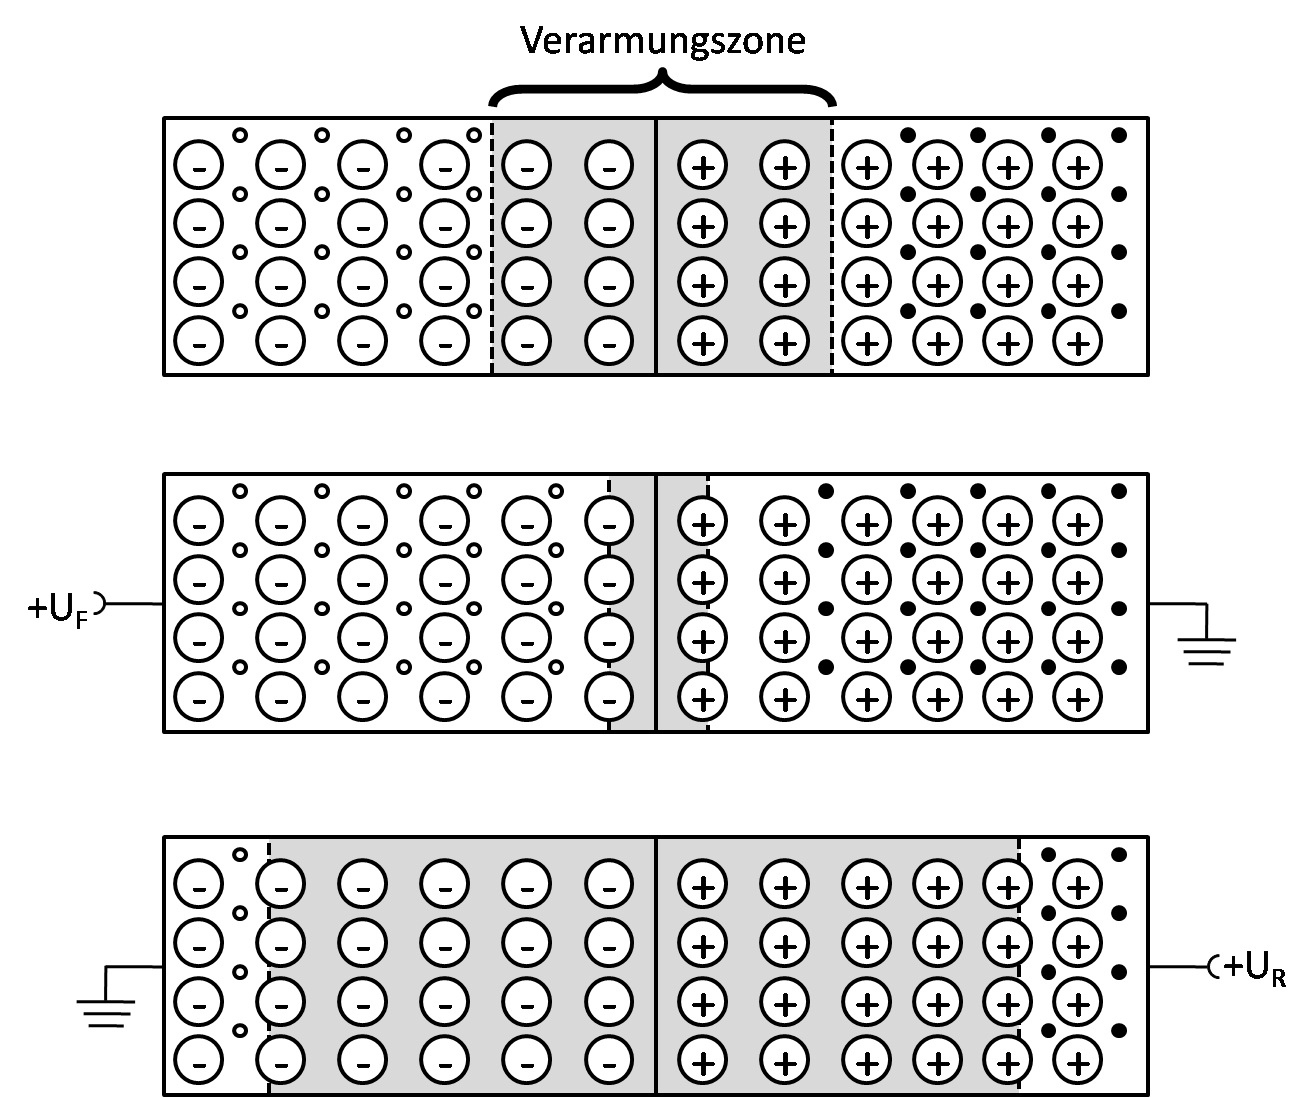
\includegraphics[width=0.45\textwidth]{Abbildungen/pn_Uebergang.jpg}
\end{center}
\caption{$pn$-\"Ubergang ohne angelegte Spannung (oben), mit \"ausserer Spannung in Durchlaß- (Mitte) und Sperrrichtung (unten).}
\label{fig:Verarmung}
\end{figure}

\subsubsection{Durchbruch}

Im Sperrbetrieb k\"onnen hohe elektrische Felder in der Sperrschicht
auftreten. Durch den {\it Lawineneneffekt} kommt
es zu einem starken Anstieg des {\it Sperrstroms}. Diesen Effekt bezeichnet 
man als {\it Durchbruch} des $pn$-\"Ubergangs.\\

\noindent
\textbf{Lawineneffekt.} 
%
Elektronen, welche durch thermische Anregung in der Sperrschicht entstehen,
werden durch das elektrische Feld beschleunigt. Bei ausreichender
Energie k\"onnen Elektronen aus Atomverb\"anden herausgeschlagen
werden. Diese sekund\"aren Elektronen k\"onnen ihrerseits durch
St\"osse Atome ionisieren und sorgen damit f\"ur einen ansteigenden
Strom.

\subsection{Ladungsdeposition in der verarmten Diode}

Geladene Teilchen (Elektronen, Myon, etc.) und Licht (Photonen) geben über verschiedene Prozesse Energie ab, wenn sie durch ein Material fliegen. Beim Halbleiter erzeugt diese Energie durch Ionisation Paare von Elektronen und Löchern, welche sich im Kristall frei bewegen können. Im elektrischen Feld, welches in der Verarmungszone herrscht, werden diese Ladungen zu den Elektroden hin beschleunigt und erzeugen so einen Strom durch die Diode und den außen angeschlossenen Stromkreis.\\
Je nach den benutzten Materialien der Diode, ihrer Dicke und der Anzahl an Teilchen oder Photonen, die die Diode pro Sekunde treffen, kann dieser Strom groß genug werden, um technisch genutzt werden zu können. Das ist das Prinzip der Solarzelle.

\subsection{Solarzellen}

Man kann sich eine Solarzelle als aus einer Stromquelle und einer Diode zusammengesetzt vorstellen. Dabei hängt die Stromstärke von der Beleuchtung ab. Wenn man die Solarzelle verdunkelt, dann misst man die Kennlinie einer Diode. Die Kennlinie einer beleuchteten Solarzelle ist daher lediglich um den Kurzschlussstrom $I_k$ nach unten verschoben (siehe Abbildung unten).\\ %\ref{fig:Kennlinienfeld}).\\
\begin{figure}[h]
	\centering
		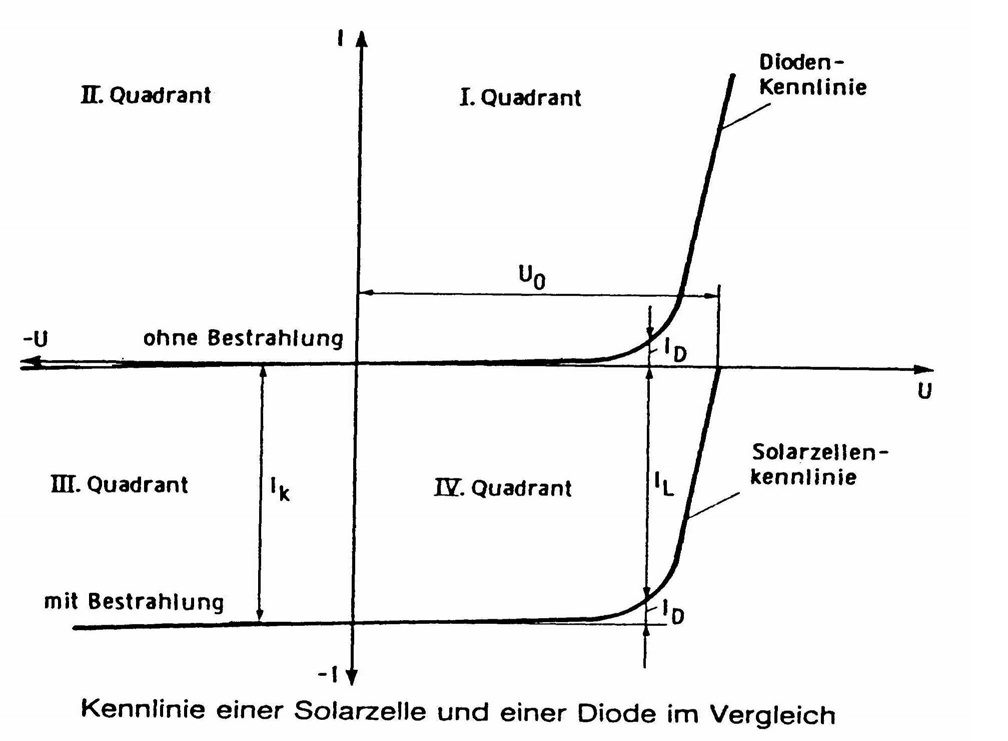
\includegraphics[width=0.5\textwidth]{Abbildungen/Kennlinienfeld.jpg}
	\label{fig:Kennlinienfeld}
\end{figure}

Da bei Beleuchtung der Solarzelle in der Regel nur der vierte Quadrant der Darstellung interessiert, wird auch nur dieser gezeichnet. Trägt man die abgegebene Leistung $P$ über der Spannung auf, kann man ein Maximum ablesen, das als Maximum Power Point bezeichnet wird (siehe Abbildung nächste Seite).\\ %\ref{fig:Leistung}).\\
Schaltet man Solarzellen in Serie, addieren sich die Spannungen, während sich der Strom nicht ändert. Bei Parallelschaltung addieren sich dagegen die Ströme, wobei die Spannung erhalten bleibt. Solarzellen werden daher zu leistungsfähigen Modulen zusammen geschaltet.\\
Im Versuch wird ein in aus 19 Einzelelementen geschaltetes Solarmodul verwendet.

\begin{figure}[h]
	\centering
		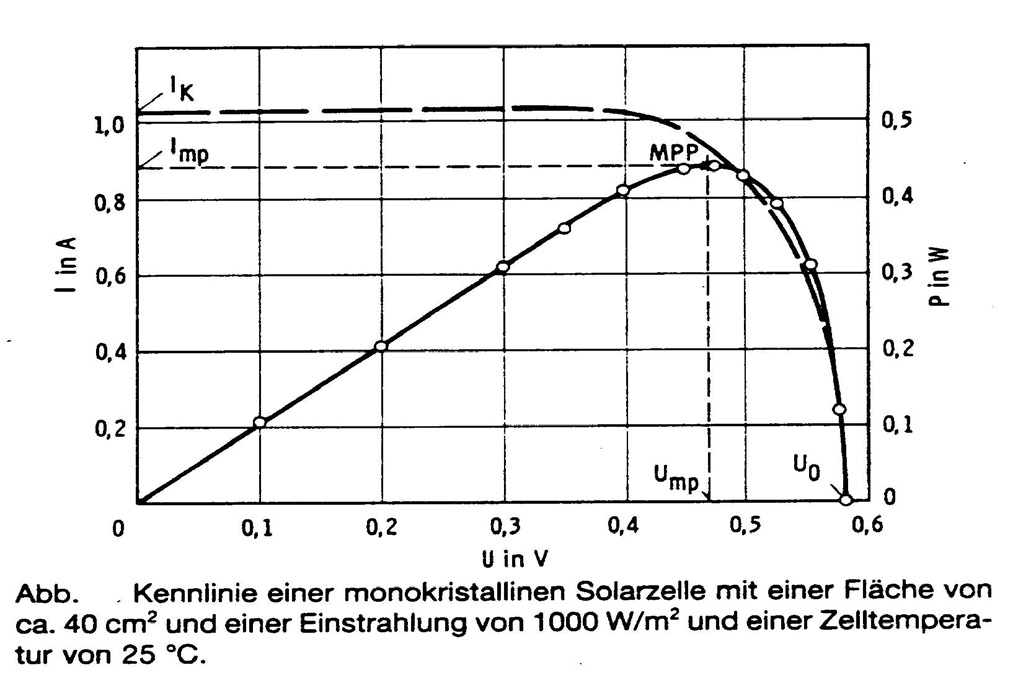
\includegraphics[width=0.5\textwidth]{Abbildungen/Leistung.jpg}
	\label{fig:Leistung}
\end{figure}

%------------------------------------------------
\section{Fragen zur Vorbereitung}
%------------------------------------------------

\begin{enumerate}
	%
	%\item Was soll heute im Praktikum gemessen werden? Warum?
	%
	\item Was sind Valenz- und Leitungsband eines elektrischen Leiters?
	%
	\item Wie schaltet man ein Volt- oder Amperemeter in einen elektrischen Schaltkreis?
	%
	\item Was ist die Energielücke zwischen Valenz- und Leitungsband?
	%
	\item Was versteht man unter Löchern im Valenzband? Wie tragen sie zum Ladungstransport bei?
	%
	\item Was versteht man unter der Dotierung eines Halbleiters? Nennen Sie ein Beispiel!
	%
	\item Was sind Akzeptor- / Donatorniveaus im Bändermodell eines Halbleiters? Wie wirken sie auf die Energielücke im Halbleiter?
	%
	\item Was passiert beim Zusammenbringen eines p- und eines n-dotierten Halbleiters mit den freien Ladungsträgern?
	%
	\item Was ist die Diffusionsspannung (auch Diodenflussspannung)?
	%
	\item Was bedeutet Schaltung in Sperr- / Flussrichtung?
	%
	\item Wie sieht die I(U)-Kennlinie der Diode aus? %Was ist die Antidiffusionsspannung?
	%
	\item Was ist eine Solarzelle? Wie erzeugt sie eine elektrische Spannung (Stichwort: Elektronen-Loch-Paar Erzeugung)?
	%
	\item Wie sieht die I(U)-Kennlinie einer Solarzelle im Vergleich zu einer gewöhnlichen Diodenkennlinie aus? Wie unterscheiden sie sich?
	%
	\item Was ist der Maximal Power Point im P(U)-Diagramm einer Solarzelle?
	%
\end{enumerate}

%------------------------------------------------
\section{Durchführung} 
%------------------------------------------------

\begin{figure}[h]
	\centering
		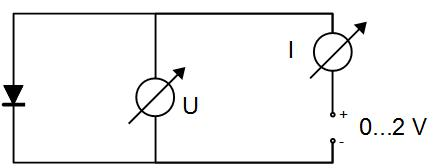
\includegraphics[width=0.5\textwidth]{Abbildungen/Schaltung_Kennlinie.jpg}
	\label{fig:Schaltung_Kennlinie}
	\caption{Schaltung zur Messung der Kennlinie der Halbleiterdiode.}
\end{figure}

\begin{enumerate}
	%
	\item \textbf{Die Kennlinie einer unbeleuchteten Halbleiterdiode:}\\
		Bauen Sie die oben skizzierte Schaltung auf, um die I(U)-Kennlinie der unter dem Plexiglashalter montierten Diode zu messen. Wählen Sie im Bereich 0\,V - 0.4\,V Schritte von 0.1\,V und im Bereich von 0.4 V\,- 0.8\,V Schritte von 0.02\,V und bestimmen Sie daraus die Diodenspannung $U_{\mathrm{D}}$.\\
		\begin{minipage}{0.6\textwidth}
		\textbf{Achtung: }\\
		Keine Spannung über 2\,V anlegen (Schalter auf der Versuchsbox)!\\
		Wenn die Überlastwarnleuchte aufleuchtet wird dies im Protokoll vermerkt und die Messung abgebrochen.\\
		Vor dem Einschalten den Assistenten fragen!
		\end{minipage}
		\begin{minipage}{0.4\textwidth}
			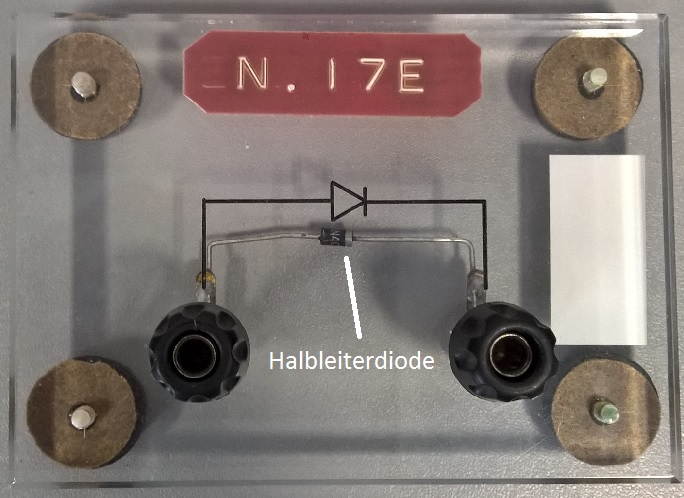
\includegraphics[width=0.8\textwidth]{Abbildungen/Diode.jpg}
			\label{fig:Bild15}
		\end{minipage}
	%
	\item \textbf{Die Kennlinie einer unbeleuchteten Solarzelle:}\\
		Ersetzen Sie die Diode durch das Solarmodul.\\
		Verdunkeln Sie die auf dem Abschirmgehäuse aufgesteckte Solarzelle mit einem der optischen Filter und messen Sie die I(U)-Kennlinie im Bereich von 0\,V bis etwa 10\,V in Schritten von 1\,V.
	%
 
	\begin{minipage}{0.6\textwidth}
			\item \textbf{Die Kennlinie einer beleuchteten Solarzelle:}\\
		Ersetzen Sie das Netzgerät durch den regelbaren Lastwiderstand und entfernen Sie den Filter.
	\end{minipage}
	\begin{minipage}{0.4\textwidth}
				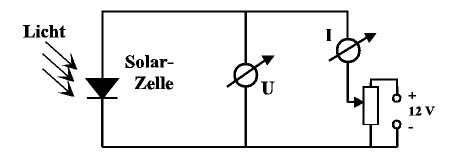
\includegraphics[width=1.00\textwidth]{Abbildungen/solarzelle.jpg}
				\label{fig:solarzelle }
		\end{minipage}
	%
	\item \textbf{Die Kennlinien einer spektral gefiltert beleuchteten Solarzelle:}\\
		Setzen sie nacheinander die verschiedenen Spektralfilter in das Abschirmgehäuse ein. Nehmen Sie die Kennlinien für blaues, grünes und gelbes Licht von 0\,V bis 5\,V in 1\,V-Schritten, darüber hinaus in 0.2\,V-Schritten auf.
\end{enumerate}

\begin{figure}[h]
	\centering
	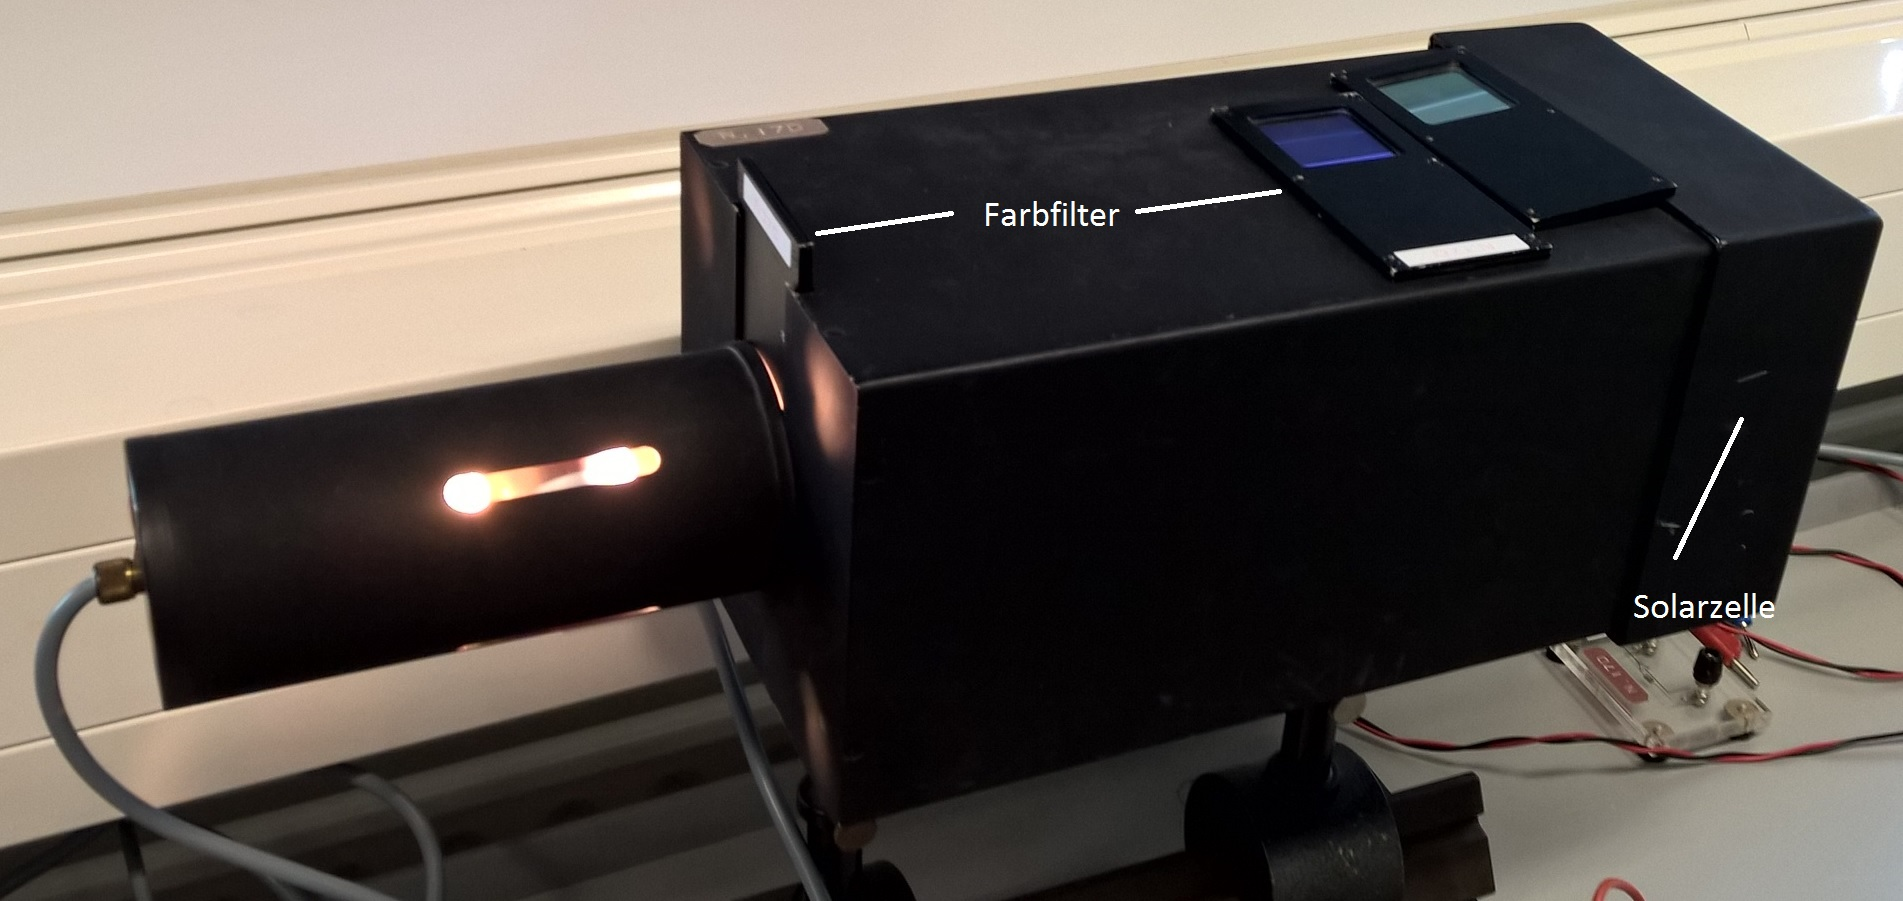
\includegraphics[width=0.7\textwidth]{Abbildungen/Solarzelle_gross.jpg}
	\caption{Die Solarzelle ist zusammen mit der Lampe in diese Box eingebaut, um Lichteinfall von außen abzuschirmen. Auf der Box liegen die Farbfilter.}
\end{figure}

%------------------------------------------------
\section{Auswertung} 
%------------------------------------------------

\etodo{Musterauswertung}

Die Diodenkennlinie lässt sich für kleinere Ströme annäherungsweise durch die Schottky-Gleichung beschreiben:
\begin{equation}
I = I_{Sp}\cdot\left(\exp\left(\frac{eU}{kT}\right)-1\right)
\end{equation}
Dabei ist $I_{Sp}$ der Sperrstrom, $e$ die Elementarladung, $k$ die Boltzmannkonstante, $T$ die absolute Temperatur (in Kelvin gemessen) und $U$ die Spannung, die über Anode und Kathode der Diode anliegt. Die Diodenspannung $U_D$ entspricht dem Schnittpunkt der U-Achse mit der Geraden, durch die man den steil ansteigenden Teil der Diodenkennlinie im Durchlassbereich approximiert.

\begin{enumerate}
	%
	\item Zeichnen Sie die $I(U)$-Kennlinien der Halbleiterdiode und bestimmen Sie aus der Auftragung graphisch die Diodenflussspannung $U_D$ mit Fehler!
	%
	\item Zeichnen Sie die $I(U)$-Kennlinien der unbeleuchteten Solarzelle und bestimmen Sie aus der Auftragung graphisch die Diodenflussspannung $U_D$ mit Fehler!
	%
	\item Tragen Sie die $I(U)$-Kennlinien aus Versuchsteil 3 und 4 auf und bestimmen Sie daraus den Kurzschlussstrom $I_k$ sowie die Leerlaufspannung $U_L = U (I = 0)$. Dazu müssen Sie gegebenenfalls den Graphen extrapolieren. 	
		Auch diese Größen sind mit Fehlern behaftet, schätzen Sie diese daher grob ab!
	%
	\item Bestimmen Sie die von der Solarzelle abgegebenen Leistungen $P = U \cdot I$ für die vier mit Beleuchtung gemessenen Kennlinien und tragen Sie diese in einen Graphen über der Spannung $U$ auf. Aus den Graphen wird der Maximal Power Point abgelesen $(P_{max}$, $I(P_{max})$ und $U(P_{max}))$. Berechnen Sie den Fehler mithilfe der Fehlerfortpflanzung, s. Kapitel \ref{chap:Fehlerfortpflanzung}. Sie können davon ausgehen, daß die Messgerätegenauigkeit bei 1\% des Messwertes liegt.
	%
	\item Die spektrale Empfindlichkeit $S$ der Solarzelle soll überprüft werden. Dazu wird das Verhältnis der spektralen Empfindlichkeiten bei gelbem (Wellenlänge $\lambda$ = 670\,nm) und grünem (Wellenlänge $\lambda$ = 530\,nm)
		Licht gebildet und mit dem Literaturwert (siehe Diagramm: \textit{Empfindlichkeit gegen Wellenlänge einer Photodiode}) für dieses Verhältnis verglichen.
		\begin{equation}
			\frac{S_{Gelb}}{S_{Gruen}}=\frac{\frac{I_K(Gelb)}{P_{Lampe}(Gelb)}}{\frac{I_k(Gruen)}{P_{Lampe}(Gruen)}}
		\end{equation}
		Hier sind $I_k$ die Kurzschlussströme der Solarzelle für die verschiedenen Filter, $P_{Lampe}$ ist die Strahlungsleistung der Lampe.
\end{enumerate}
Beim verwendeten Aufbau ist die Strahlungsleistung der Lampe mit dem gelben Filter $P_{Lampe}(Gelb)$ um 10\% größer als bei Verwendung des grünen Filters ($P_{Lampe}(Gruen)$). Daher benötigen Sie nicht die absolute Leistung der Glühlampe.

\noindent
Da die Intensität des Sonnenlichts bei etwa 880\,nm maximal ist, baut man Solarzellen so, dass sie in diesem Bereich ihre maximale Empfindlichkeit haben. Je weiter man sich von diesem Maximum entfernt, umso geringer wird auch die Empfindlichkeit (Messung 3).

\begin{minipage}{0.5\textwidth}
	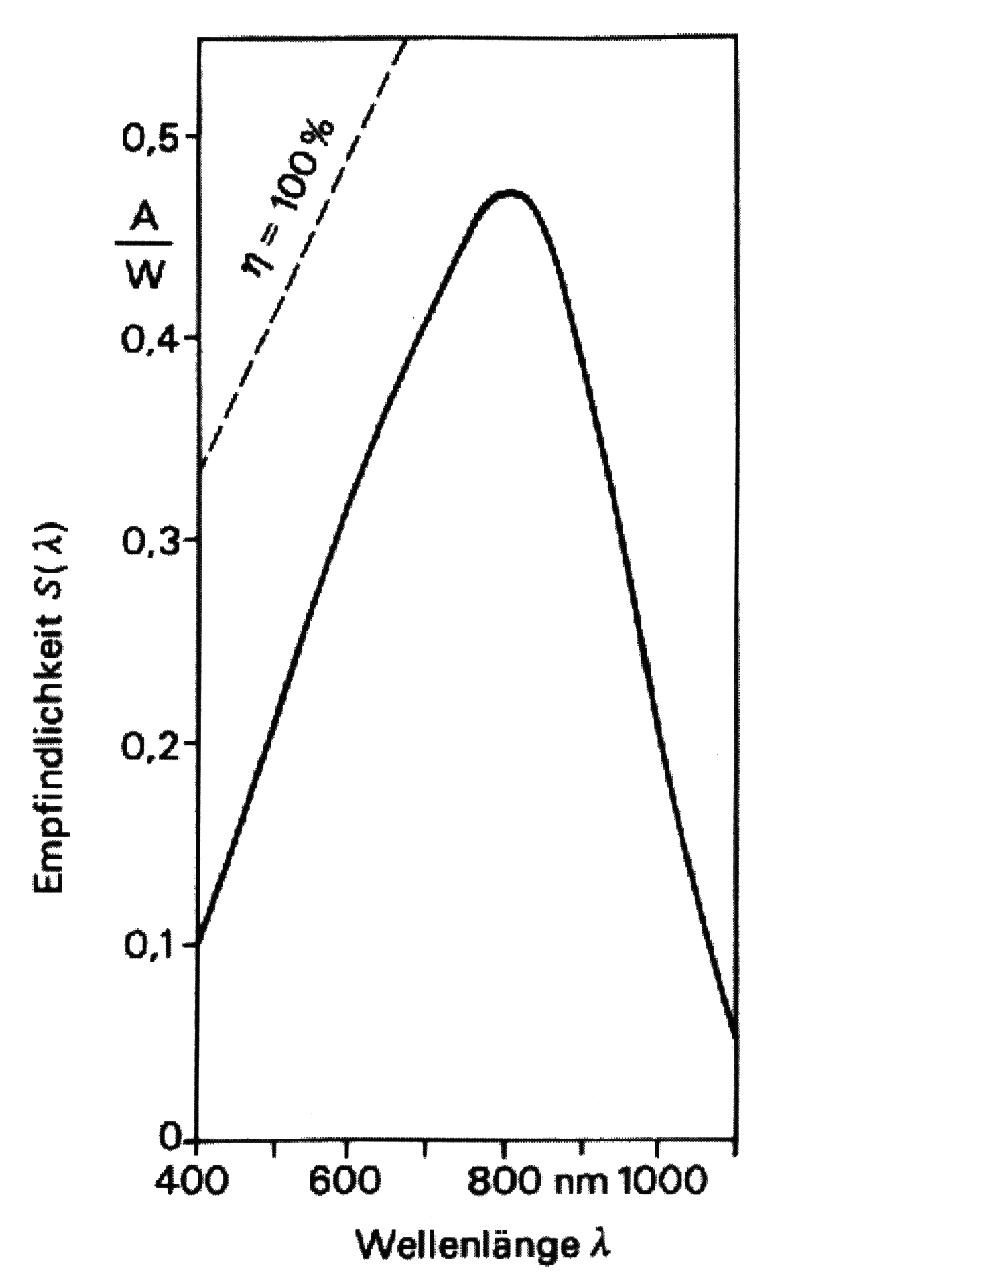
\includegraphics[width=1.00\textwidth]{Abbildungen/QE_Solarzelle.JPG}
	\label{fig:BILD17}
\end{minipage}
\begin{minipage}{0.5\textwidth}
Das nebenstehende Bild zeigt die Empfindlichkeit einer Si-Photo-Diode in Abhängigkeit von der Wellenlänge. Gestrichelt eingezeichnet ist der Verlauf der Empfindlichkeit einer idealen Diode mit einer Ausbeute von 100\%.
Die gemessene Kurve liegt generell tiefer, verläuft aber bei kurzen Wellenlängen etwa parallel zur theoretischen Kurve.
Der steile Abfall auf der langwelligen Seite kommt daher, dass die Photonen nicht mehr genügend Energie haben, um Elektronen über die Bandlücke anzuregen.
\end{minipage}

\end{document}	% Solarzelle und Hlableiterdiode
%\chapter{Transistor}
\label{v:18}

In diesem Versuch soll die grundlegende Funktion als Leistungsverstärker eines Transistors studiert werden.

%------------------------------------------------
\section{Stichworte}
%------------------------------------------------

Halbleiter; $pn$-Übergang; Wirkungsweise eines Transistors; Emitterschaltung; Transistorkennlinie; Transistor als Verstärker.
%
%------------------------------------------------
\section{Literatur}
%------------------------------------------------

Gehrtsen, Kapitel 14.4.1-3
%
%------------------------------------------------
\section{Anwendungsbeispiele}
%------------------------------------------------

Transistoren gehören zu den wichtigsten elektronischen Bauelementen. Sie werden zum Verstärken und Schalten elektrischer Signale verwendet. Meist bestehen sie aus drei Zonen von halbleitendem Material, das verschieden dotiert ist (p- oder n-leitend). Diese Dreiteilung erinnert noch an ihre Vorläufer, die Trioden. Daher existieren in der Nomenklatur auch viele Ähnlichkeiten. Diese Vakuum-Röhren, deren Funktion man meist schneller begreift, erhalten ihre beweglichen Ladungsträger (Elektronen) aus einem Heizdraht, sie werden auf eine positiven Elektrode hin beschleunigt und können durch ein dazwischen liegendes Gitter abgebremst oder durchgelassen werden. Im Transistor bewegen sich die (negativen oder positiven) Ladungsträger durch Festkörpergrenzflächen, wieder geregelt durch Ladungen, die von außen beeinflusst werden.\\
Eine Vielzahl von Transistoren oder anderen Bauelementen (z.B. Widerstände) können in einem einzigen Fertigungsprozess auf einem einkristallinen Siliziumplättchen (Chip) hergestellt werden. Vor einigen Jahren überschlugen sich die Computer-Chip Hersteller noch mit Angaben, wie viel Tausend Transistoren auf einem Quadratzentimeter Platz hätten. Heute ist es um diese Zahlen still geworden, weil sie so astronomisch groß geworden sind, dass man sie nur noch in Zehnerpotenzen angeben kann, die dann aber doch keiner mehr begreift.\\
Es lohnt sich, sich mit diesem, zugegebenermaßen komplizierten, Bauelement näher zu beschäftigen, das in allen Regelungen und Computern steckt und schon unsichtbar klein geworden ist und unser Leben im letzten Jahrhundert so grundlegend geändert hat.

%------------------------------------------------
\section{Theoretischer Hintergrund}
%------------------------------------------------

\subsection{Der (unbelastete) Spannungsteiler}

	\begin{figure}[h!]
		\centering
		\begin{circuitikz}
			\begin{scope}[xshift=0cm]
				\draw (2.5,2)
					to [R, i<_=$I$, l=$R_1$](0,2) 
					to [V_=$U_o$] (0,0) 
					to [short] (2.5,0) coordinate (B)
					to [R, l=$R_2$] (2.5,2) coordinate (A);
				\draw (A) to [short, *-o] ++(0.5,0) coordinate (A1);
				\draw (A1) node [anchor=south] {$A$};
				\draw (B) to [short, *-o] ++(0.5,0) coordinate (B1);
				\draw (B1) node [anchor=north] {$B$};
				\draw (B1) to [open, v=$U_{AB}$] (A1);
			\end{scope}
		\end{circuitikz}
		\caption{Spannungsteiler}
		\label{fig:spannungsteiler}
	\end{figure}
Schaltet man, wie in Abbildung \ref{fig:spannungsteiler}, zwei Widerstände $R_1$ und $R_2$ hintereinander (in Serie), so fließt durch beide Widerstände derselbe Strom $I$. Die Spannung $U_0$, die die Spannungsquelle zur Verfügung stellt, fällt über beide Widerstände ab nach dem Ohm'schen Gesetz $U_0 = R\cdot I = \left( R_1 + R_2\right)\cdot I$. Über jeden einzelnen Widerstand fällt also nur ein Teil der gesamten Spannung ab: $U_0 = U_1 + U_2 = R_1\cdot I + R_2\cdot I$.\\
Diese \textit{Spannungsteiler} genannte Schaltung wird häufig benutzt, wenn man an einen Verbraucher nicht die ganze Spannung $U_0$ anlegen will oder darf. Stattdessen schließt man den Verbraucher zum Beispiel an die Klemmen $A$ und $B$ an, so dass an ihm die Spannung $U_{AB}$ liegt. Wie groß diese Spannung ist, kann man nun aus den obigen Gleichungen berechnen. Diese folgen aus den sogenannten Kirchhoff'schen Gesetzen, die Sie in Versuch \ref{v:13} genauer kennenlernen.\\
Für den Fall, dass der Verbraucher nicht viel Strom zieht, die Spannung $U_{AB}$ wie folgt berechnet werden kann:
\begin{equation}
	U_{AB} = U_0\cdot\frac{R_2}{R_1 + R_2}
\end{equation}
In diesem Versuch werden Sie die Spannungsteilerschaltung benutzen, um mehrere verschiedene, variable Spannungen an die Anschlüsse des Transistors anzulegen, obwohl nur ein einziges Netzgerät zur Verfügung steht.

\subsection{Der Bipolartransistor}

Werden zwei Elektronen-Halbleiter (n-Leiter) durch eine Schicht eines Löcher-Halbleiters (p-Leiter) getrennt, deren Schichtdicke in der Größenordnung der Ausdehnung des an den Grenzflächen aufgebauten elektrischen Feldes liegt 
($10^{-5}$ m), so kann ein Teil der Elektronen durch die Schicht hindurchtreten. Das Ausmaß des durchtretenden Teiles hängt von der Stärke des elektrischen Feldes ab. Dieses Feld kann von aussen durch Anlegen einer elektrischen Spannung an die dünne Schicht beeinflusst werden. Damit wird der Durchtritt der Elektronen steuerbar!\\
Der Strom $I_C$, der durch den Transistor fließt, lässt sich durch den Basisstrom $I_B$ steuern. Die Verstärkerwirkung des Transistors beruht darauf, dass im Sättigungsbereich der Transistorkennlinie kleine Änderungen des Basisstroms große Änderungen des Kollektorstroms bewirken.\\

\noindent
Die dünne Schicht, Basis $B$ genannt, übernimmt damit ähnliche Funktion wie das Gitter der Triodenröhre. Der an die Basis Elektronen abgebende n-Leiter heißt Emitter $E$. Er hat eine ähnliche Funktion wie die Kathode in der Triodenröhre. Der Elektronen aufnehmende Teil heißt Kollektor $C$ und entspricht der Anode in der Triodenröhre.\\
Das beschriebene System ist ein npn-Transistor. Mit p werden die positiven Ladungsträger (Löcher) der Basis $B$, symbolisiert, während n für die negativen Ladungsträger (Elektronen) im Emitter $E$ und im Kollektor $C$ steht. Ein pnp-Transistor funktioniert analog, aber mit umgekehrten Vorzeichen der Ladungen, Ströme und Spannungen.\\

\noindent
Dieser Transistor hat zwei pn-Übergänge und man kann ihn sich stark vereinfacht als zwei entgegengesetzt geschaltete Dioden vorstellen (siehe Abbildung).\\
In der sog. Emitterschaltung (s. Versuchsaufbau) ist die E-B-Diode in Durchlassrichtung geschaltet, d.h. Elektronen können von E nach B gelangen und es fließt ein (kleiner) Basisstrom. Der Kollektor liegt gegenüber der Basis auf positivem Potential, also ist die C-B-Diode in Sperrrichtung geschaltet. Der Strom $I_C$ ist der Sperrstrom der C-B-Diode und ist abhängig von der Anzahl der Elektronen in der p-leitenden Basis (s. Versuch \ref{v:17}). Da die B-E-Diode in Durchlassrichtung geschaltet ist, hängt die Elektronenkonzentration in der Basis von der äußeren Spannung $U_{BE}$ bzw. vom Basisstrom $I_B$ ab. Dadurch ist der Kollektorstrom $I_C$ eine Funktion sowohl von der äußeren Spannung $U_{EC}$ zwischen Emitter und Kollektor als auch vom Basisstrom $I_B$: $I_C = I_C (U_{EC} , I_B)$\\

\noindent
Sehr stark vereinfachend kann man sich einen Transistor in dieser Beschaltung, bei konstanter Kollektor-Emitter-Spannung $U_CE$, also ähnlich wie eine Stromquelle vorstellen, deren Ausgangsstrom durch die zwischen Basis und Emitter angelegte Spannung $U_{BE}$ eingestellt werden kann.\\
Eine der angenehmen Eigenschaften der Bipolartransistoren ist, dass der Kollektorstrom $I_C$ linear vom Basisstrom abhängt:
\begin{equation}
	I_C = \beta\cdot I_B\; .
\end{equation}
Den Proportionalitätsfaktor $\beta$ bezeichnet man als Stromverstärkungsfaktor des Transistors. Dieser hängt vom genauen Aufbau des Transistors ab, also der Breite der Basiszone und den Ladungsträgerkonzentrationen in den verschieden dotierten Bereichen, und kann somit von Transistor zu Transistor signifikant unterschiedlich sein.

%------------------------------------------------
\section{Fragen zur Vorbereitung}
%------------------------------------------------

\begin{enumerate}
	%
	%\item Was soll heute im Praktikum gemessen werden? Warum?
	%
	\item Was ist eine Spannungsteilerschaltung?
	%
	\item Wozu kann ein Transistor benutzt werden? Nennen Sie Beispiele!
	%
	\item Aus welchen Halbleitern wird ein Transistor aufgebaut?
	%
	\item Wie sind die Spannungen an den einzelnen Schichten bei der im Versuch verwendeten Emitterschaltung geschaltet?
	%
	\item Was versteht man unter Basis, Emitter und Kollektor?
	%
	\item Wie funktioniert ein Transistor in Emitterschaltung? Welche entscheidende Rolle spielt dabei die Basis?
	%
	\item Welcher Strom kann mit dem Basisstrom geregelt werden?
	%
	\item Wie sehen die Ausgangskennlinien eines Transistors in Emitterschaltung aus? Von welchem Parameter hängen die Kennlinien ab?
	%
	\item Was vergleicht man mit dem Verstärkungsfaktor eines Transistors? Wie berechnet sich der Verstärkungsfaktor des Transistors?
	%
\end{enumerate}

%------------------------------------------------
\section{Durchführung} 
%------------------------------------------------

\begin{figure}[h]
	\centering
		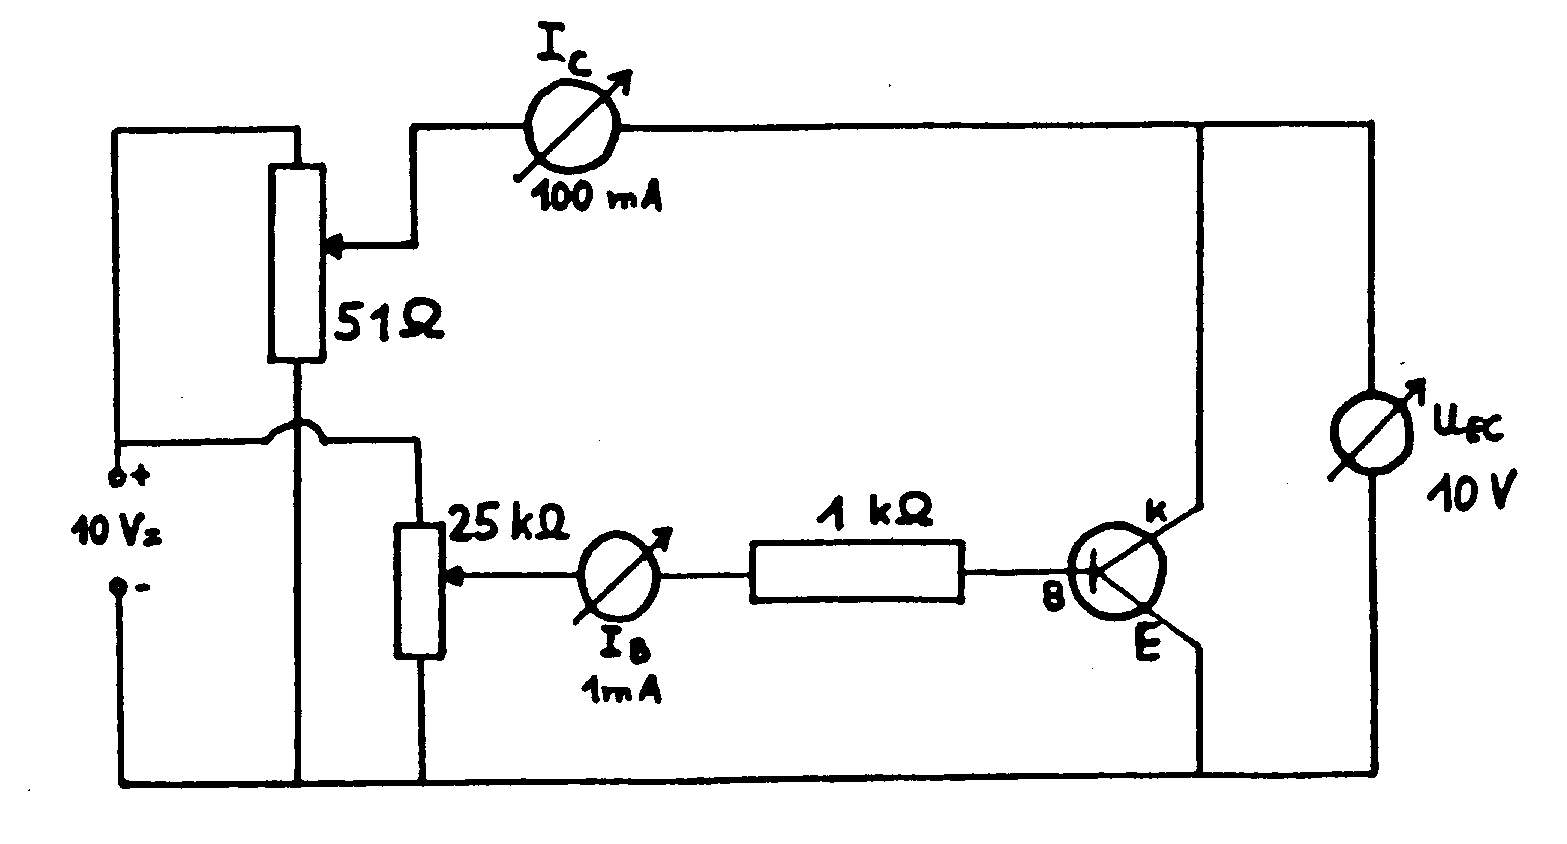
\includegraphics[width=0.75\textwidth]{Versuch_17-18/Abbildungen/BILD23.JPG}
	\label{fig:BILD23}
\end{figure}

\begin{enumerate}
	%
	\item Bauen Sie die Schaltung gemäß des Schaltplanes auf und lassen sie diese vom Assistenten kontrollieren.
	%
	\item Stellen sie einen Basisstrom $I_B$ von 0.2\,mA ein. Messen Sie den Kollektorstrom $I_C$ in Abhängigkeit von der Spannung $U_{EC}$ ($U_{EC}$ = 0, 0.1, 0.2, 0.3, 0.4, 0.5\,V anschließend 1\,V, 2\,V, 3\,V, ..., 10\,V).
		Regeln Sie dabei den Basisstrom $I_B$ immer nach.
	%
	\item Wiederholen Sie die Messung für verschiedene Basisströme $I_B$ = 0.3, 0.4, 0.5\,mA.
	%
\end{enumerate}

%------------------------------------------------
\section{Auswertung} 
%------------------------------------------------

\begin{enumerate}
	%
	\item Tragen Sie das Ausgangskennlinienfeld $I_C (U_E)$ für die vier Basisströme auf.
	%
	\item Entnehmen Sie aus Ihren Messreihen zu jedem Basisstrom $I_B$ die Werte des Kollektorstoms $I_C$ bei einer Spannung $U_{EC}$ = 8\,V. Tragen Sie diese auf und bestimmen sie graphisch den Verstärkungsfaktor $\beta$ mit Fehler.
\end{enumerate}	% Transistor
\documentclass[11pt, twoside, a4paper]{book}

\usepackage{graphicx}
\usepackage[utf8]{inputenc}
\usepackage{ngerman}
%\usepackage{lineno}
\usepackage{verbatim}
\usepackage[squaren]{SIunits}
\usepackage{amsmath}
\usepackage{amsfonts}
\usepackage{amssymb}
\usepackage{enumitem}
\usepackage{fancyhdr}
\usepackage{textcomp}
\usepackage{subcaption}
\usepackage[noadjust]{marginnote}
\usepackage{tikz}
\usepackage{nicefrac}
\usepackage{framed}
\usepackage{import}

\usetikzlibrary{calc,intersections}
\usetikzlibrary{arrows}
\usetikzlibrary{decorations.markings}
\usetikzlibrary{decorations.pathreplacing}
\usepackage[european resistors]{circuitikz}
\usepackage[ 
    top=2cm, 
    bottom=2cm, 
    outer=3cm, 
    inner=3cm,
    marginparwidth=2.5cm,
		headheight=14pt
  ]{geometry}

\usepackage{parskip}
\usepackage{pdfpages}

\setlength{\parindent}{0pt}

\newcommand{\experimentheader}[4]
{
  \iftutor{{\bf Schwierigkeitsgrad:} #1\\}
  \iftutor{{\bf Dauer:} #2\\}
  {\bf Ger\"ate:} #3\\
  {\bf Bauteile:} #4
}

\newcommand{\hintboxNone}{0}
\newcommand{\hintboxExclamation}{1}
\newenvironment{hintbox}[4][\hsize]
{
  \def\FrameCommand
  {%
    {\color{#3}\vrule width 3pt}%
    \hspace{0pt}%must no space.
    \fboxsep=\FrameSep\colorbox{#4}%
  }%
  \MakeFramed{\hsize#1\advance\hsize-\width\FrameRestore}%
  \mbox{\textbf{#2}:}%
}
{
  \endMakeFramed
}
\newcommand{\xhintbox}[3]
{
  \begin{hintbox}{Achtung}{red!50}{red!10}
    #3
  \end{hintbox}
}

\newenvironment{hint}
{
  \begin{hintbox}{Hinweis}{green!50}{green!10}
}
{
  \end{hintbox}
}

\newenvironment{definition}
{
  \begin{hintbox}{Definition\\}{white!50}{white!10}
}
{
  \end{hintbox}
}

\newenvironment{important}
{
  \begin{hintbox}{Hinweis}{gray!50}{gray!10}
}
{
  \end{hintbox}
}

\newenvironment{jason}
{
  \begin{hintbox}{Achtung}{red!50}{red!10}
}
{
  \end{hintbox}
}

\newcommand{\mandatoryenumi}
{
  \renewcommand{\labelenumi}{\arabic{enumi}.} 
}
\newcommand{\optionalenumi}
{
  \renewcommand{\labelenumi}{$\bigstar$\quad\arabic{enumi}.} 
}
\newcommand{\mandatoryenumii}
{
  \renewcommand{\labelenumii}{(\alph{enumii})} 
}
\newcommand{\optionalenumii}
{
  \renewcommand{\labelenumii}{$\bigstar$\quad(\alph{enumii})} 
}
\newcommand{\icname}[1]{\mbox{\tt #1}}


  %\newcommand{\iftutor}[1]{}
\newcommand{\ifnotutor}[1]{#1}

  \newcommand{\iftutor}[1]{#1}
\newcommand{\ifnotutor}[1]{}


\newenvironment{tutorhint}{\comment}{\endcomment}
\newenvironment{todo}{\comment}{\endcomment}
\newenvironment{solution}{\comment}{\endcomment}
\iftutor
{
  \renewenvironment{todo}
  {
    \hintbox{Todo}{red!50!yellow!90}{red!50!yellow!20}
  }
  {
    \endhintbox
  }
  \renewenvironment{tutorhint}
  {
    \hintbox{Tutorenhinweis der Stunde}{blue!50}{blue!10}
  }
  {
    \endhintbox
  }
  \renewenvironment{solution}
  {
    \hintbox{L\"osung}{black!80}{black!5}
  }
  {
    \endhintbox
  }
}
\newcommand{\etutorhint}[1]
{
  \iftutor{
    \tutorhint
      #1
    \endtutorhint
  }
}
\newcommand{\esolution}[1]
{
  \iftutor
  {
    \solution
    #1
    \endsolution
  }
}
\newcommand{\etodo}[1]
{
  \iftutor
  {
    \todo
    #1
    \endtodo
  }
}



\begin{document}

\renewcommand{\thechapter}{\arabic{chapter}}
\setcounter{chapter}{0}
\def\chaptername{Versuch}

\chapter{Stoss}
\label{v:1}

In diesem Versuch werden die Grundlagen des inelastischen Sto{\ss}es am Beispiel eines Fadenpendels studiert. Das Fadenpendel ist auch heute noch eines der genauesten Instrumente zur Bestimmung der Erdbeschleunigung.

%\noindent
%{\bf Kenntnisse}: ???

%------------------------------------------------
\section{Stichworte}
%------------------------------------------------
Hubarbeit; Fadenpendel; pot. und kinet. Energie; Energiesatz; Impulssatz; elast. und inelast. Sto{\ss}.
%
%------------------------------------------------
\section{Literatur}
%------------------------------------------------
Gehrtsen, Kapitel 1.4.2/3, 1.5.2 bis 1.5.9; Demtr"oder, Kapitel 2.1, 2.2, 4.2
%
%------------------------------------------------
\section{Anwendungsbeispiele}
%------------------------------------------------
%
Beim inelastischen Stoß zweier Körper wird ein Teil der zur Verfügung stehenden Energie (die Summe der kinetischen Energien der beiden Körper vor dem Stoß) in Innere Energie der Körper umgewandelt. Das kann durch Erwärmung oder Verformung der Körper geschehen.\\
Beispiele für solche inelastischen Stoßvorgänge sind die Formung chemischer Verbindungen aus mehreren Atomen oder Molekülen in Gasen oder Flüssigkeiten, das Auffalten von Gebirgen beim Zusammensto{\ss} tektonischer Platten oder auf kleineren Skalen der Blechschaden beim Zusammensto{\ss} von Fahrzeugen. Ein weiteres Beispiel ist die mit der Zeit abnehmende Sprunghöhe eines elastischen Balls, der vom Boden abprallt.\\
Wir betrachten inelastische Stöße am Beispiel des Fadenpendels, anhand dessen sehr viele Eigenschaften von schwingenden Systemen verdeutlicht werden können. Einer der interessantesten Aspekte ist zum Beispiel die Unabhängigkeit der Schwingungsdauer des Pendels von der Masse des schwingenden Körpers, s. Pendeluhren oder Spiderman.\\

Auch wenn die theoretische Einleitung etwas länger ist als bei anderen Versuchen, ist es doch sinnvoll sich mit den Grundlagen der Bewegung von Massepunkten (geworfene Bälle, Sie, Autos, etc.) zu beschäftigen. Diese Gesetzmäßigkeiten betreffen nicht nur jeden einzelnen von uns im Alltag, sondern bilden die Grundlagen für Effekte in allen Naturwissenschaften.
%
%------------------------------------------------
\section{Theoretischer Hintergrund}
%------------------------------------------------

\subsection{Die Kinematik von Massepunkten}

Die Kinematik ist die Lehre der Bewegung von Punkten und K"orpern im Raum, beschrieben durch die Gr"o{\ss}en Position, Geschwindigkeit und Beschleunigung.\\
Den Gr"o{\ss}en Position, Geschwindigkeit und Beschleunigung bei einer geradlinigen Bewegung entsprechen bei einer Drehbewegung die Gr"o{\ss}en Winkel, Winkelgeschwindigkeit und Winkelbeschleunigung.

Die Position eines Punktes wird durch drei Koordinaten im dreidimensionalen Raum festgelegt. Bei einem starren K"orper (der sich nicht verformt) gen"ugen drei weitere Freiheitsgrade f"ur die Rotation (Drehungen im dreidimensionalen Raum), um die Lage des gesamten K"orpers zu beschreiben. Die drei Koordinaten eines Ortes stellt man durch die drei Komponenten eine Vektors dar:\\
Die Koordinaten (x,y,z) entsprechen dem Ort $\vec{x} = (x,y,z)$. Mit der Schreibweise $\vec{x}(t)$ bezeichnet man den Ort des K"orpers zu einer bestimmten Zeit $t$. Tr"agt man nun diese Funktion gegen die Zeit $t$ auf, so bekommt man die sogenannte \textit{Bahnkurve} des K"orpers. Geschwindigkeit und Beschleunigung sind definiert als Ableitungen der Ortskurve nach der Zeit:
\begin{align}
\vec{v}(t) & = \dot{\vec{x}}(t) = \frac{d\vec{x}(t)}{dt} = \left(\frac{dx}{dt}, \frac{dy}{dt}, \frac{dz}{dt}\right) \\
\vec{a}(t) & = \ddot{\vec{x}}(t) = \frac{d^2\vec{x}(t)}{dt^2} = \left(\frac{d^2x}{dt^2} , \frac{d^2y}{dt^2}, \frac{d^2z}{dt^2}\right)
\end{align}

\subsection{Grundlagen von Schwingungen}

Verschiebt man einen elastisch gebundenen Körper aus seiner Ruhelage (z. Bsp. an einer Feder herabhängende Masse nach oben oder unten, die Masse eines Fadenpendels zur Seite), dann bewegt er sich nach dem Loslassen beschleunigt auf seine Ruhelage zu und läuft aufgrund seiner Trägheit über diese hinaus. Nach dem Durchgang durch die Ruhelage wirkt die rücktreibende Kraft verzögernd, da sie jetzt der Bewegungsrichtung entgegengesetzt ist und der Körper kommt schließlich zur Ruhe (Umkehrpunkt). Jetzt wiederholt sich der Bewegungsablauf in umgekehrter Richtung, bis der Ausgangspunkt erreicht ist (wenn Reibung vernachl"assigt wird). \\
Diesen periodisch wiederkehrenden Vorgang nennt man Schwingung, die Zeit $T$, die verstreicht bis sich ein Bewegungszustand (bestimmt durch Ort, Betrag und Richtung der Geschwindigkeit) wieder einstellt, hei{\ss}t Schwingungsdauer. Die Frequenz einer Schwingung ist definiert durch
\begin{equation}
f = 1/T \; ,
\end{equation}
ihre Kreisfrequenz $\omega$, auch Winkelfrequenz genannt, durch
\begin{equation}
\omega = 2\pi f = 2\pi /T\; .
\end{equation}
%
\begin{hint}
Winkel werden entweder in Einheiten von Grad oder von Radiant angegeben. In der alltäglich gebräuchlicheren Einheit entspricht eine volle Umdrehung um eine Achse 360° (Grad).\\
Das Rechnen mit Winkeln wird allerdings sehr viel einfacher, wenn man diese in der dimensionslose Einheit von Radiant angibt. In dieser Einheit entspricht eine volle Umdrehung $2\pi$~rad. Die Umrechnung von Winkeln in Grad nach Radiant ist gegeben durch
\begin{equation}
	\varphi \mathrm{\left[rad\right]} = \varphi \mathrm{\left[grad\right]}*\frac{2\pi}{360^{\circ}} \; .
\end{equation}
Die oben eingeführte Frequenz $f$ gibt an, wie oft pro Sekunde ein kompletter Schwingungsvorgang durchlaufen wird. Beim Fadenpendel zum Beispiel, wie oft sich das Pendel vom linken Umkehrpunkt zum rechten und zurück bewegt. Die Kreisfrequenz $\omega$ hingegen gibt an, welcher Anteil des gesamten Schwingungsvorgangs pro Sekunde zurückgelegt wird.\\Die Einheit der Frequenz ist das \textit{Hertz}, mit $1 \mathrm{H} = 1/\mathrm{s}$, während die Einheit der Kreisfrequenz \textit{Radiant pro Sekunde} ist.
\end{hint}
%
Man unterscheidet zwischen harmonischen und anharmonischen Schwingungen, je nachdem, ob die r"ucktreibende Kraft linear oder nichtlinear von der Auslenkung abh"angt. Eine Schwingung, deren Amplitude durch Energieverlust (zum Beispiel aufgrund von Reibung) monoton abnimmt, hei{\ss}t ged"ampfte Schwingung. Sie ist kein periodischer Vorgang, da der Ausgangspunkt der Bewegung nicht wieder erreicht wird. Erzwungene Schwingungen sind solche, bei denen durch Energiezufuhr von au{\ss}en ein System zum schwingen angeregt bzw. trotz D"ampfung in einem station"aren Schwingungszustand gehalten wird.

Man kann auch die Energie des Pendels im Verlauf einer Pendelschwingung betrachten. Wird das Pendel ausgelenkt, so wird der K"orper dadurch ein wenig angehoben. Da dabei Arbeit gegen die Schwerkraft verrichtet wird, hat der K"orper im angehobenen Zustand, also wenn das Pendel ausgelenkt ist, eine gr"o{\ss}ere potenzielle Energie, als wenn es nicht ausgelenkt ist. Die zus"atzliche potenzielle Energie betr"agt $E_{pot} = m\cdot g\cdot h = m\cdot g\cdot l(1-\cos\varphi)$. In diesem Moment bewegt sich der K"orper nicht, so dass er keine kinetische Energie besitzt.\\
Wird der K"orper nun losgelassen wird er in einer beschleunigten Bewegung auf die Ruhelage zu fallen. In dem Moment, wo der K"orper die Ruhelage passiert, seine H"ohe "uber dem Erdboden also wieder dieselbe ist wie vor der Auslenkung, hat er kein zus"atzliche potenzielle Energie mehr. Stattdessen bewegt er sich hier mit seiner maximalen Geschwindigkeit $v_{max}$. Demnach hat er die kinetische Energie $E_{kin} = \frac{1}{2}m\cdot v_{max}^2$. \\
Die gesamte zus"atzliche potenzielle Energie, die der K"orper in der ausgelenkten Position hatte, ist in diesem Moment komplett in kinetische Energie verwandelt.

\subsection{Das Fadenpendel}

Das Fadenpendel besteht aus einer Kugel der Masse $m$, die an einem Faden der L"ange $L$ (gemessen zwischen Aufh"angepunkt und Mittelpunkt der Kugel) h"angt. Wenn die Masse des Fadens vernachl"assigbar ist gegen $m$ und der Durchmesser der Kugel sehr klein gegen"uber der Fadenl"ange L ist, hei{\ss}t die Anordnung \emph{mathematisches Pendel}, weil $m$ als Punktmasse behandelt werden kann.\\
Die Bewegung des Pendels unter dem Einfluss der Schwerkraft kann man sich wie folgt klarmachen:\\ 
An der aus der Ruhelage um den Winkel $\varphi$ herausgedrehten Kugel greift die Schwerkraft $\vec{F}_s = m\vec{g}$ an. Man zerlegt die Schwerkraft in zwei Komponenten
\begin{itemize}
 \item eine radiale Komponente $F_r$, die im gespannten Faden eine gleich gro{\ss}, entgegengerichtete Kraft hervorruft und deshalb nichts zur Beschleunigung beitr"agt,
 \item eine tangentiale Komponente $F_t = -m\cdot g\cdot\sin\varphi$, die eine Tangentialbeschleunigung \\
 $a_t = -g\cdot\sin\varphi$ bewirkt. Dies ist die r"ucktreibende Kraft.
\end{itemize}
%
In ebenen Polarkoordinaten lautet die Bewegungsgleichung des Pendels:
\begin{equation}
m\cdot g\cdot\sin\varphi = -m\cdot L\cdot \ddot{\varphi}
\end{equation}
%
Entwickelt man $\sin\varphi$ in die Taylorreihe
\begin{equation*}
\sin\varphi = \varphi - \frac{\varphi^3}{3!}+ \frac{\varphi^5}{5!} - \frac{\varphi^7}{7!}+ ...
\end{equation*}
so kann man f"ur gen"ugend kleine Werte von $\varphi$ die h"oheren Glieder vernachl"assigen. Damit wird die Bewegungsgleichung zu:
\begin{equation}
\ddot{\varphi} = - \frac{g}{L}\cdot\varphi \; .
\end{equation}
Die L"osung dieser Differentialgleichung ist die Funktion
\begin{equation}
\varphi (t) = \varphi_0\cdot\sin\omega t \;.
\end{equation}
%
$\varphi_0$ ist dabei die ursprüngliche Winkelauslenkung. Die Kreisfrequenz der Schwingung ist dabei $\omega = \sqrt{g/L}$, die Schwingungsdauer oder \emph{Periode} der Schwingung wird $T = \frac{2\pi}{\omega} = 2\pi\cdot\sqrt{L/g}$. Wie man sieht, ist die Periode also nicht von der Auslenkung oder der Masse abhängig, sondern nur von der Fadenlänge und der Erdbeschleunigung.

Diese Tatsache ist die Grundlage der Funktion von Pendeluhren, welche im 18. Jahrhundert besonders in der Seefahrt eine große Rolle spielten, weil sie zum die objektive Zeitmessung auf hoher See, und damit die genaue Bestimmung des Längengrades erlaubten. Das englische Parlament hatte im Jahr 1714 ein Preisgeld von 20.000 Pfund für die Lösung des sogenannten Längenproblems (die genaue Bestimmung des aktuellen Längengrades) ausgelobt, welches sich der Tischler, Erfinder und autodidaktische Uhrmacher John Harrison erst im Jahre 1765 nach langem Streit teilweise ausgezahlt bekam. Die von ihm erfundene Uhr erreichte eine damals enorm hohe Genauigkeit (etwa 1 Sekunde Abweichung pro Monat).
%
\begin{figure}[hb]
	\centering
		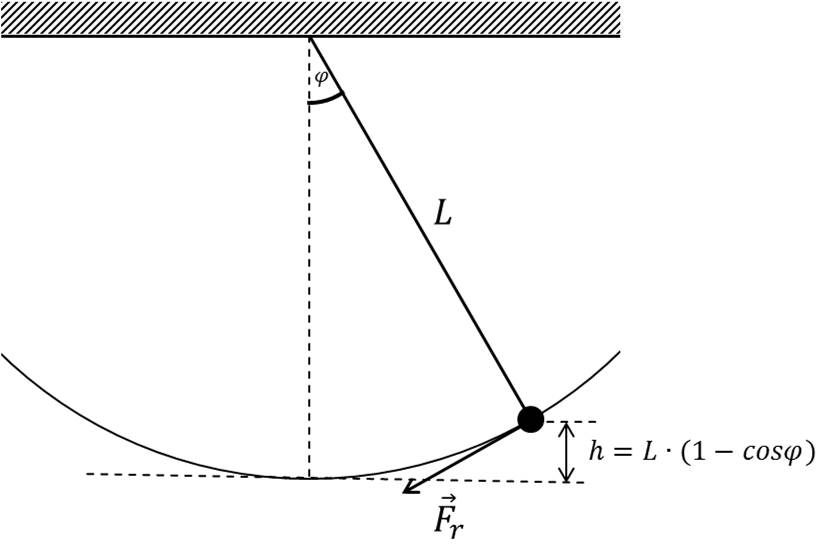
\includegraphics[height=6cm]{figures/Fadenpendel.jpg}
	\caption{Fadenpendel}
	\label{fig:Fadenpendel}
\end{figure}

\subsection{St"o{\ss}e zwischen zwei K"orpern}

Ein Stoß ist eine sehr kurzzeitige Wechselwirkung zwischen zwei Körpern. Vor und nach dem Stoß bewegen sich beide, ohne einander zu beeinflussen. Obwohl die Gesamtenergie der beiden Sto{\ss}partner immer erhalten ist, kann h"aufig ein Teil der kinetischen Energie beim Sto{\ss} in andere Energieformen, z.B. in potenzielle Energie oder in W"armeenergie umgewandelt werden. Der Gesamtimpuls der beiden bleibt jedoch beim Sto{\ss} immer erhalten. Die Grundgleichungen f"ur Sto{\ss}prozesse zwischen zwei K"orpern lassen sich also schreiben als:
\begin{align}
\vec{p}_1^{'} + \vec{p}_2^{'} &= \vec{p}_1 + \vec{p}_2 &\mathrm{Impulssatz}\\
\frac{p_1^{'2}}{2m_1} + \frac{p_2^{'2}}{2m_2} &= \frac{p_1^{2}}{2m_1} + \frac{p_2^{2}}{2m_2} &\mathrm{Energiesatz}
\end{align} 
%
Hierbei bezeichnen gestrichene Gr"o{\ss}en (z.B. $\vec{p}_1^{'}$) auf die Gr"o{\ss} nach dem Stoss. Beachten Sie, dass wir bei dieser klassischen Form des Energiesatzes die innere Energie nicht ber"ucksichtigt haben.\\
%
\begin{hint}
	Es sei an die Definitionen von kinetischer Energie und Impuls erinnert:
	\begin{align}
		\vec{p} &= m\cdot\vec{v}\\
		E_{kin} &= \frac{1}{2}mv^2 
	\end{align}
\end{hint}
%
Anhand der Energien der beiden Stoßpartner unterscheidet man drei Situationen:
\begin{enumerate}
	\item \textbf{Elastischer Stoß:}\\
		Die kinetische Energie beider Stoßpartner ist nach dem Stoß genauso groß wie davor. Beispiele hierfür sind die meisten Zusammenstöße von Molekülen, roten Blutkörperchen oder ähnlichem, die Rammbockkämpfe vieler Tierarten, oder die Brown'sche Bewegung.
	%
	\item \textbf{Inelastischer Stoß:}\\
		Ein Teil der kinetischen Energie der Stoßpartner wird dauerhaft in eine andere Energieform überführt, wie zum Beispiel Erwärmung oder Verformung. Beispiele hierfür wären die Überdehnung einer Sehne oder der Bruch eines Knochens, chemische Reaktionen, oder das Hämmern eines Spechts.
	%
	\item \textbf{Vollständig inelastischer Stoß:}\\
		Hierbei verbinden sich die Stoßpartner miteinander, sodass sie sich im Folgenden mit einer gemeinsamen Geschwindigkeit weiterbewegen. Beispiele sind die Untereinheiten von Ribosomen, die sich miteinander verbinden, sowie die beiden Metallkugeln im Versuch, welche nach dem Stoß durch die Knetmasse verbunden sind.
	%
\end{enumerate}
%------------------------------------------------
\section{Fragen zur Vorbereitung}
%------------------------------------------------

\begin{enumerate} 
% \item Was soll heute im Praktikum gemessen werden? Warum?
 %
 \item Welche mechanischen Gr"o{\ss}en ben"otigt man, um die Bewegung eines K"orpers zu beschreiben?
 %
 \item Wie stehen Ort, Geschwindigkeit und Beschleunigung eines K"orpers im Zusammenhang?
 %
 \item Wie lauten die Formeln f"ur die kinetische und die potentielle Energie?
 %
 \item Warum gilt beim inelastischen Stoss nur der Impuls-, nicht aber der Energiesatz?
 %
 \item Wie kommt die Formel $L=\frac{T^2\,g}{4\,\pi^2}$ zustande?
 %
 \item Wie lautet das Gravitationsgesetz?
\end{enumerate} 

%------------------------------------------------
\section{Durchführung} 
%------------------------------------------------

Die Masse der großen Kugel beträgt $M = 2,10$\,kg, die der kleinen Kugel beträgt $m=0,11$\,kg.

\begin{enumerate}
%
\item Bestimmen Sie die Schwingungsdauer T des Pendels, indem Sie fünfmal die Zeit für 10 ganze Schwingungen messen. Die horizontale Auslenkung des Pendels soll dabei nicht größer sein als etwa 40~cm. Warum? Wie groß ist der Fehler Ihrer Messung? \label{Mess:Schwingungsdauer}
%
\item An der großen Kugel wird die Knetmasse so befestigt, dass die ausgelenkte kleine Kugel zentral auf die Knetmasse stößt und dann beide Kugeln samt Knetmasse nach dem unelastischen Stoß gemeinsam ausschwingen. Die Auftreffgeschwindigkeit der kleinen Kugel wird variiert, indem man die Fallhöhe $h$ verändert ($h$ = 3, 4, 5, 6~cm). In Abhängigkeit von der Fallhöhe $h$ der kleinen Kugel ist dann der maximale Ausschlag x$_0$ der beiden Kugeln samt Knetmasse nach dem zentralen Stoß zu messen. Schätzen Sie den Fehler Ihrer Messung ab.
\label{Mess:inelast_Stoss}
%
\item Messen Sie die Masse der Knetmasse $m_k$. Wie groß ist die Unsicherheit?
%
\item Notieren Sie die Länge des Fadens, an dem der Pendelkörper aufgehängt ist. Diese können Sie als genau bekannt annehmen.
%
\end{enumerate}

%------------------------------------------------
\section{Auswertung} 
%------------------------------------------------
\etodo{Musterauswertung}
\begin{enumerate}
%
\item Berechnen Sie aus der Messung \ref{Mess:Schwingungsdauer} die Erdbeschleunigung $g$. Wie gro{\ss} ist der Fehler Ihrer berechneten Größe? Siehe hierzu Kapitel \ref{chap:Fehlerfortpflanzung}. Vergleichen Sie diese mit dem Literaturwert und diskutieren Sie Gr"unde m"oglicher Abweichungen.
%
\item In Abh"angigkeit von der Fallh"ohe $h$ berechne man die Geschwindigkeit $v_m$ der kleinen Kugel beim Auftreffen auf die gro{\ss}e Kugel.
%
\item Nach dem inelastischen Stoss bewegen sich alle Massen (einschlie{\ss}lich Knete!) mit einer gemeinsamen Geschwindigkeit $v_{th}$. Berechnen Sie diese Geschwindigkeit mithilfe des Impulssatzes 
\begin{equation}
\label{Gl:Impulssatz}
(M + m + m_k)\cdot v_{th} = m\cdot v_m\; .
\end{equation}
(Machen Sie sich klar, dass Gleichung \ref{Gl:Impulssatz} wirklich dem Impulssatz entspricht.)
%
\item Bestimmen Sie die Geschwindigkeit $v_{exp}$ der beiden Massen samt Knete aus dem maximalen Ausschlag $x_0$ in Messung \ref{Mess:inelast_Stoss} für alle Fallhöhen. Benutzen Sie die Beziehung:
\begin{equation}
v_{exp} = \frac{2\pi}{T}\cdot x_0\
\end{equation}
%
\item Vergleichen Sie die experimentellen und die theoretischen Geschwindigkeiten $v_{exp}$ und $v_{th}$ miteinander und geben Sie eine Erklärung für auftretende Differenzen ( = Fehlerbetrachtung).
%
\end{enumerate}

\end{document}			% Sto�

\chapter{Wechselstrom und R-C-Kreis}
\label{v:15}

In diesem Versuch lernen Sie die Grundlagen der Funktion und Bedienung eines Digital-Speicher-Oszilloskops (DSO), sowie die Auf- und Entladekurve eines Kondesnators kennen.

%------------------------------------------------
\section{Stichworte}
%------------------------------------------------

Kathodenstrahl; Braun'sche Röhre; Oszillograph; Ablenkung im elektrischen Feld; Wechselspannung; Kondensator; Kapazität.
%
%------------------------------------------------
\section{Literatur}
%------------------------------------------------

Gehrtsen, Kapitel 7.5.2/3, 8.2.1, 8.2.3
%Teile übernommen aus der Anleitung \textit{''Oszilloskop und Funktionsgenerator''} der Universität Oldenburg
%
%------------------------------------------------
\section{Anwendungsbeispiele}
%------------------------------------------------

R ist die Abkürzung (Symbol) für den elektrischen Widerstand, C für die Kapazität eines Kondensators und L für die Induktivität einer Spule; R-C-Kreise sind Kombinationen aus Widerständen und Kondensatoren, die ein für viele physikalische Vorgänge charakteristisches exponentielles Abklingverhalten zeigen. R-L-Kreise, aus Widerstand und Spule aufgebaut, zeigen auf vereinfachte Weise, was passiert wenn bei den meisten Haushaltsgeräten die Spannung eingeschaltet wird (z. Bsp. Glühbirnen).\\

Eine Zellmembran mit geringer Leitfähigkeit als Grenzschicht zwischen gut leitenden elektrolytischen Flüssigkeiten stellt eine elektrische Parallelschaltung eines Widerstandes (Membranwiderstand) und eines Kondensators (Membrankapazität) dar. Aus der Anwendung entsprechender physikalischer Modellvorstellungen kann ein Verständnis der physiologischen Vorgänge und Messtechniken zur Untersuchung von Zelleigenschaften und interzellulären Vorgängen gewonnen werden.

%------------------------------------------------
\section{Theoretischer Hintergrund}
%------------------------------------------------

\subsection{Oszilloskop}

\begin{figure}[hb]
	\centering
		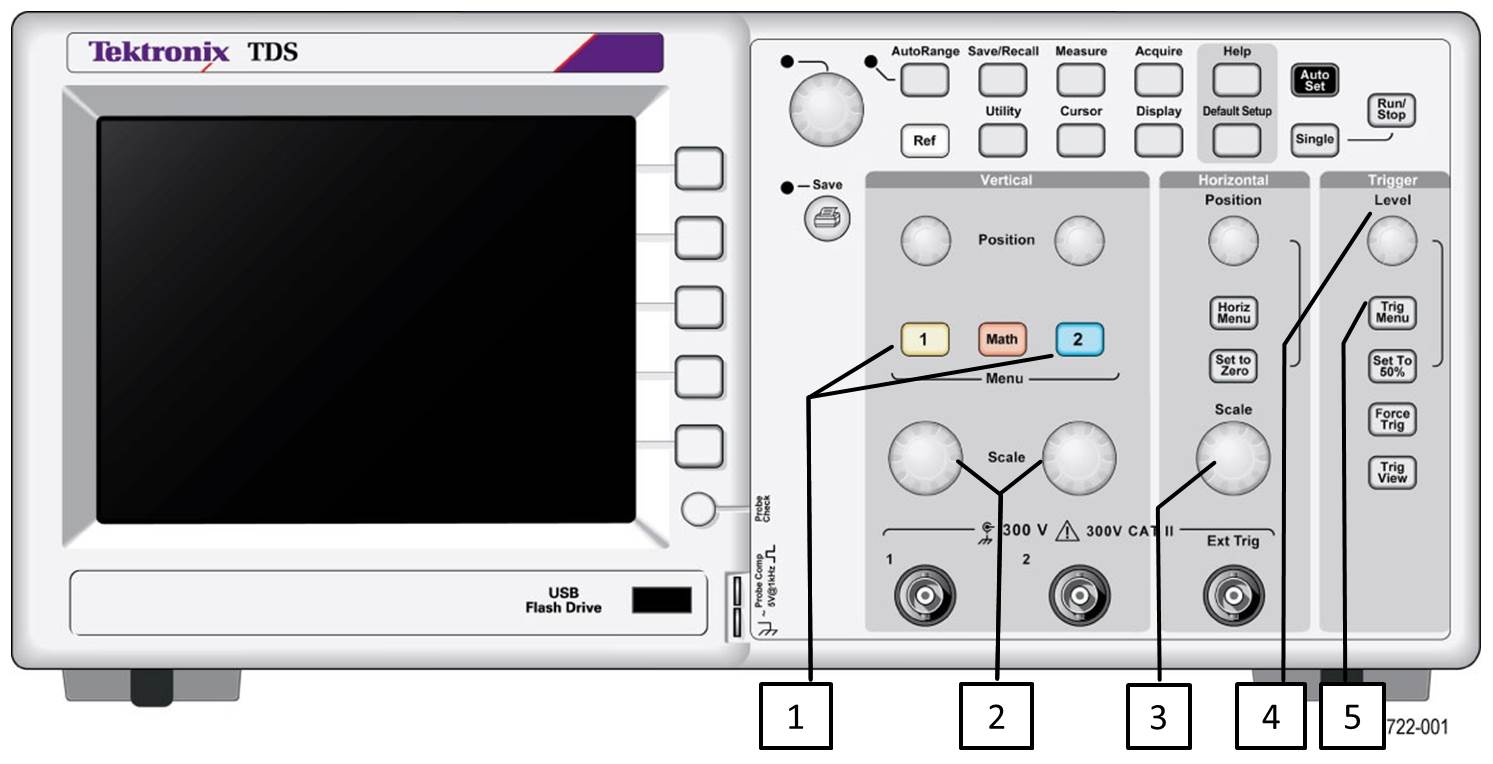
\includegraphics[width=0.5\textwidth]{Versuch_15-16/Abbildungen/TDS2000.JPG}
	\caption{Front des TDS 2001C.}
	\label{fig:TDS2000}
\end{figure}

%Das Oszilloskop ist das vielseitigste Messgerät im Bereich der Elektrik und Elektronik. Es dient der Beobachtung und Messung zeitabhängiger, schneller und wiederkehrender elektrischer Signale. Bis vor einigen Jahren waren noch hauptsächlich analoge Elektronenstrahl-Oszilloskope im Einsatz, die inzwischen jedoch weitestgehend von Digital-Speicher-Oszilloskopen verdrängt wurden. Dennoch wollen wir mit einer kurzen Beschreibung der Funktionsweise des Elektronenstrahl-Oszilloskops beginnen, diese viele grundlegende Funktionen des Oszilloskops anschaulich erklärt.
%
%\begin{figure}[h!]
	%\centering
		%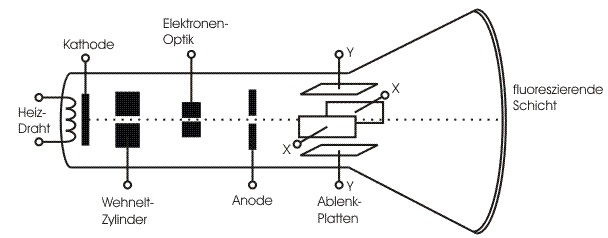
\includegraphics[width=0.5\textwidth]{Versuch_15-16/Abbildungen/Elektronenstrahlroehre.jpg}
	%\caption{Aufbau der Elektronenstrahlröhre des Oszilloskops.}
	%\label{fig:Elektronenstrahlroehre}
%\end{figure}
%
%Kernstück eines Oszilloskops ist eine Elektronenstrahlröhre, die einen Strahl beschleunigter Elektronen als quasi trägheitslosen Zeiger auf einen szintillierenden Schirm schießt. Zur Auslenkung dieses Strahls in der vertikalen Y Richtung wird dabei die zu untersuchende Eingangsspannung an die Platten eines Ablenkkondensators gelegt, so dass die Elektronen im elektrischen Feld des Kondensators abgelenkt werden.\\
%Um die zeitliche Abhängigkeit der Eingangsspannung darzustellen, wird eine linear steigende (Sägezahn-)Spannung (Kippspannung) an die horizontalen Ablenkplatten gelegt, sodass der Elektronenstrahl mit gleichbleibender Geschwindigkeit die X Achse überstreicht.\\
%Verschieden schnelle Signale können über Änderungen der Frequenz der Sägezahnspannung dargestellt werden (Einstellknopf 'SEC/DIV', 2 in Abbildung \ref{fig:TDS2000}). Signale mit verschiedener Amplitude können durch Anpassung der Verstärkung der Eingangsspannung sichtbar gemacht werden (Einstellknopf 'VOLTS/DIV', 1 in Abbildung \ref{fig:TDS2000}).\\
%Ein Trigger-Netzwerk sorgt dafür, dass die Zeitbasis immer in dem Moment ''angestoßen'' wird, in dem das Signal am Y-Eingang erscheint und damit Signal und Zeitbasis synchronisiert werden. Für ein wiederkehrendes Signal erhält man auf diese Weise ein stehendes Bild auf dem Bildschirm des Oszilloskops.\\
%

%
%\noindent
%Auf der Frontseite des hier benutzten TDS2001C Oszilloskops erkennt man 3 Bedienfelder:\\
%Im linken Teil findet man die Einstellungen für die Verstärkung der Eingangssignale der beiden Kanäle (2), sowie die Knöpfe für die Kanalmenüs (1). Hier lässt sich die Einkopplung des Eingangssignals (DC), die Bandbreite des Kanals (Voll), sowie die Grob- bzw. Feineinstellung der Verstärkung einstellen. Des Weiteren findet man hier einen einstellbaren Verstärkungsfaktor für den Eingang (sollte 1X sein), sowie die Möglichkeit, das Eingangssignal zu invertieren (Aus).\\
%Im mittleren Teil finden sich die Einstellungen für die Zeitachse, welche für alle Kanäle gleich ist. Hier können Sie die Vergrößerung der Zeitachse ('SEC/DIV', Drehknopf 2) einstellen, sowie die Zeitachse hin- und herbewegen. Dabei gibt der vertikale weiße Pfeil den Zeitpunkt an, an dem die Triggerbedingung erfüllt wurde.\\
%Im rechten Teil können Sie den Spannungspegel einstellen, 
%Rechts oben im Feld befinden sich der Einschaltknopf (1), die anderen Knöpfe bestimmen die Zeitablenkung des Oszilloskops, d.h. die x-Achse des Bildes und die sog. Triggerung, d.h. den Beginn der Ablenkung des Elektronenstrahls von links nach rechts.\\
%Im unteren rechten Feld werden die zu untersuchenden Spannungen eingegeben. Dieses Gerät kann zwei Signale gleichzeitig anzeigen, daher sind viele Funktionen doppelt. Es regelt also die Y-Achse.\\
%Im schmalen linken Feld unter dem Bildschirm gibt es die Helligkeits- (18) und Schärfe-regelung (20) des Bildes, sowie weitere Testfunktionen des Gerätes.

Will man schnell laufende Vorgänge, z.B. Wechselspannungen oder Impulse, stetig messen und in Abhängigkeit von der Zeit registrieren, so verwendet man ein Oszilloskop. Dieses stellt Spannungen direkt als Funktion der Zeit dar und ermöglicht so die Beobachtung von Vorgängen mit hoher Frequenz.

  Meist benutzt man das Oszilloskop im sogenannten \textit{YT-Modus}, bei dem auf der horizontalen X-Achse des Displays die Zeit $t$ dargestellt wird. Die \textit{Zeitbasis}, d.h. die Skalierung der Zeitachse, kann durch den horizontalen Wahlschalter zwischen \unit{5}{\nano\second} pro Kästchen und \unit{50}{\second} pro Kästchen einstellen. 
  Die K\"astchen werden am Oszilloskop als DIV (f\"ur Division) bezeichnet. 
  Weitere Eigenschaften der Zeitachse können in dem Menü eingestellt werden, welches nach Drücken der 
  Taste HORIZ MENU angezeigt wird. Für die richtige Wahl der Zeitbasis sollten Sie sich klar machen, mit welcher Frequenz die Spannung am Eingang des Oszilloskops sich verändert.

  Auf der vertikalen Y-Achse wird die am Eingang gemessene Spannung dargestellt. Die Skala der Y-Achse kann über den vertikalen Wahlschalter für jeden der vier Kanäle des Oszilloskops getrennt zwischen \unit{20}{\milli\volt} pro Kästchen und \unit{50}{\volt} pro Kästchen eingestellt werden. Zur richtigen Wahl des Y-Verstärkungsfaktors sollten Sie sich klarmachen, welche Spannung Sie an der zu messenden Stelle Ihrer Schaltung erwarten. 

  \paragraph{Kanaleigenschaften}
  Weitere Eigenschaften der Y-Achse können im sogenannten \textit{Kanalmenü} eingestellt werden, welches nach Drücken der Taste CH MENU für den entsprechenden Kanal angezeigt wird. Diese Eigenschaften können für die beiden Kanäle unabhängig von einander eingestellt werden. 
  \begin{itemize}
    \item KOPPLUNG: Es ist möglich, über eine zum Eingang in Reihe geschaltete Kapazität, den Gleichspannungsanteil der Eingangsspannung zu unterdrücken. Dies geschieht, wenn die Kopplung des Kanals auf AC gestellt wird. Dieser Modus ist nützlich, um Spannungsänderungen zu untersuchen und beschleunigt die Arbeit mit dem Oszilloskop erheblich,
      falls der Gleichspannungsanteil tats\"achlich irrelevant ist.
      \begin{important}
        Während des Versuchs stellen Sie die Kopplung bitte auf DC.
      \end{important}

    \item BANDBREITE: Die Bandbreiteneinstellung bestimmt die frequenzabhängig Unterdrückung von Eingangssignalen. Wenn Sie Signale in der Gößenordnung MHz darstellen wollen, sollten Sie darauf achten, dass die Bandbreite auf den maximalen Wert für den Oszilloskoptyp eingestellt ist, da ansonsten die Signalform stark verzerrt dargestellt wird.
    \item TASTKOPF: Die Tastköpfe, mit denen Sie Ihre Schaltung untersuchen, können die Eingangsspannung über einen einstellbaren Spannungsteiler um den Faktor 10 unterdrücken. Dies dient dazu, größere Spannungen auf dem Oszilloskop darstellen zu können, als man sicher an den Eingang anschliessen könnte ohne Bauteile im Oszilloskop zu zerstören. 
    Stellen Sie sicher, dass die Unterdrückung des Tastkopfes und die im Kanalmenü eingestellte Unterdrückung übereinstimmen, da Sie ansonsten andere Spannungswerte am Oszilloskop ablesen, als wirklich in der Schaltung anliegen.
			\begin{important}
				Im Versuch stellen Sie bitte sicher, dass keine Unterdrückung (1X) eingestellt ist.
			\end{important}
    \item INVERTIERUNG: Hiermit können Sie anstelle der Spannung $U$ die invertierte Spannung $-U$ auf dem Oszilloskop darstellen. 
			\begin{important}
				Im Versuch stellen Sie bitte sicher, dass keine Invertierung eingestellt ist.
			\end{important}
  \end{itemize}

  \paragraph{Trigger} 
  Das Oszilloskop stellt die Eingangsspannung auf dem Display dar, wenn die sogenannte \textit{Triggerbedingung} erfüllt ist. Diese stellt man im Trigger Menü ein, welches nach Drücken der Taste TRIG MENU angezeigt wird. 
  Das Oszilloskop stellt mehrere verschiedene Arten von Triggerbedingungen zur Verfügung. So kann, unter anderem auf Pulse bestimmter Breite getriggert werden. Im Praktikum ist allerdings der meistbenutzte Triggertyp der sogenannte \textit{Flankentrigger}. Eine typische Triggerbedinung lautet: Triggere, wenn die Spannung am Kanal 1 einen Wert von \unit{0.1}{\volt} überschreitet.\\
  Diese Bedingung besteht aus drei separat einstellbaren Teilen:
  \begin{enumerate}
    \item Die Triggerquelle, d.h. die Spannung welches Kanals soll betrachtet werden? Wird im Triggermenü über den Punkt QUELLE eingestellt.
    \item Der Triggertyp, d.h. Eingangsspannung soll den Schwellenwert von unten überschreiten (positive oder steigende Flanke) oder von oben unterschreiten (negative oder fallende Flanke). Wird im Triggermenü über den Punkt FLANKE eingestellt.
    \item Der Schwellenwert, d.h. wie groß ist die Spannung, mit der die Engangsspannung verglichen werden soll? Wird über den Drehknopf LEVEL eingestellt.
  \end{enumerate}
  Eine weitere wichtige Eigenschaft des Triggers ist der \textit{Triggermodus} (Triggermenü, Punkt MODUS):
  \begin{itemize}
    \item Triggermodus AUTO: Das Display wird in regelmäßigen Abständen neu aufgebaut, unabhängig davon, ob die Triggerbedingung erfüllt ist. Dieser Modus eignet sich dafür, eine erste Vorstellung des Signals zu bekommen, w\"ahrend noch kein korrekter Trigger eingestellt ist.
    \item Triggermodus NORMAL: Das Display wird nur dann neu aufgebaut, wenn die Triggerbedingung erfüllt ist. Dieser Modus eignet sich, um schnelle Veränderungen der Eingangsspannung, wie zum Beispiel logische Signale, zu untersuchen.
      Ist die Triggerbedingung in kurzen Abst\"anden verl\"asslich erf\"ullt,
      verhalen sich NORMAL und AUTO identisch. Sie k\"onnen also h\"aufig im
      Modus AUTO verbleiben und nur zu NORMAL wechseln, wenn zwischen
      zwei Triggern zu viel Zeit vergeht.
    \item
      Triggermodus STOP: Das Oszilloskop beh\"alt die letzte Aufnahme.
    \item
      Triggermodus SINGLE: Falls Sie eine funktionierende Triggerbedingung haben
      und sich eine einzige Aufnahme des Eingangssignals anschauen m\"ochten,
      k\"onnen Sie auf SINGLE wechseln. Das Oszilloskop wartet dann auf eine
      Triggerbedingung, nimmt genau eine Aufnahme auf und wechselt zu STOP.
  \end{itemize}
	
\subsubsection{Betrieb}

Da wir nur auf Pos. I messen, wird der Tastkopf bei CH 1 eingesteckt, die zugehörige Massenverbindung erfolgt an der Bananenbuchse daneben.\\
Mit dem Drehknopf (2) wird die Empfindlichkeit der Y-Achse eingestellt: Stellung 2~V bedeutet, dass jedes Kästchen auf dem Bildschirm 2~V hoch ist.\\

\noindent
Alle Oszilloskope (dieser Welt ?) werden nach diesem Schema bedient. Die vielen Knöpfe verführen zum Spielen, und wir möchten alle ermutigen, zu probieren, was die einzelnen Schalter bewirken. Diese Anleitung führt - hoffentlich - wieder zu einer Schalterstellung zurück, die eine richtige Messung ermöglicht.

\subsection{Wechselspannung und Wechselstrom}

Als Wechselspannung bezeichnet man eine periodische Spannung mit sinus- oder kosinusförmigem Verlauf:
\begin{equation}
 U(t) = U_0 \sin\omega t
\end{equation}
%
Die Wechselspannung verursacht an einem Bauteil einen Wechselstrom, der eine zeitliche Versetzung $t'$ (Phasenverschiebung $\delta$) gegenüber der Spannung haben kann:
\begin{equation}
 I(t) = I_0 \sin\omega(t-t') = I_0 \sin(\omega t - \delta)
\end{equation}

\noindent
Wechselspannungen werden technisch meist durch Induktion erzeugt (Dynamogenerator). Wird eine Leiterschleife mit konstanter Winkelgeschwindigkeit in einem homogenen Magnetfeld gedreht, so wird in dieser auf Grund des Induktionsgesetzes eine Wechselspannung induziert.\\

\noindent
In Wechselstromkreisen gibt es unterschiedliche Angaben zur Charakterisierung der Größe von Spannung und Strom: die Amplituden oder Scheitelwerte ($U_0$, $I_0$), die Effektivwerte ($U_{eff}$, $I_{eff}$) und die Spitze-Spitze-Werte ($U_{SS}$):
\begin{itemize}
 %
 \item \underline{Amplitude (Scheitelwert):} Die Amplituden geben die Maxima von Spannung oder Strom an; sie entsprechen dem Amplitudenbegriff der trigonometrischen Funktionen.
 %
 \item \underline{Effektivwert:} Die Effektivwerte von Spannung und Strom sind charakteristische Werte, deren Produkt (wie im Fall des Gleichstroms) die (mittlere) joulesche Wärmeleistung ergibt:
  \begin{equation}
   \bar{P} = U_{eff}\, I_{eff} = \frac{U_0}{\sqrt{2}}\,\frac{I_0}{\sqrt{2}}
  \end{equation}
 %
 \item \underline{Spitze-Spitze-Wert:} In besonderen Fällen wird für Spannungen die Differenz zwischen größtem und kleinstem Wert als sogenannter Spitze-Spitze-Wert $U_{SS}$ angegeben.
 %
\end{itemize}

Die Amplituden und $U_{SS}$ können auf dem Oszilloskop direkt beobachtet werden. Die Effektivwerte werden mit Multimetern gemessen, die für Wechselspannungen und -ströme einen eingebauten Gleichrichter enthalten und für diese Messbereiche in Effektivwerten kalibriert sind.\\

Analog zum ohmschen Widerstand R wird als Wechselstromwiderstand Z (Scheinwiderstand oder Impedanz) das Verhältnis der Amplituden von Spannung und Strom definiert:
\begin{equation}
 Z = \frac{U_0}{I_0} = \frac{U_{eff}}{I_{eff}}
 \label{eq:Z}
\end{equation}
Bei ohmschen Widerständen stimmen Gleich- und Wechselstromwiderstand überein. Bei anderen Bauteilen, wie Kondensatoren und Spulen, ist dies nicht der Fall.

\subsection{Kondensator und R-C-Kreis}

Ein Kondensator ist ein Speicher für elektrische Ladung. Die in einem Kondensator befindliche Ladung $Q$ ($Q$ auf der einen Platte und $-Q$ auf der anderen) ist proportional zur ''Größe'' des Kondensators (Kapazität $C$) und zur Spannung $U$ (die Kapazität $C$ ist definiert als Verhältnis von Ladung zu Spannung):
\begin{equation}
 Q = C\cdot U
 \label{eq:Q}
\end{equation}

\noindent
Die Einheit der Kapazität ist:
\begin{equation}
 \mathrm{\left[C\right] = 1\frac{As}{V} = 1 F \quad (Farad)}
\end{equation}

\noindent
Der Strom $I_C$ durch den Kondensator ist die zeitliche Ableitung der Ladung, mit Gleichung (\ref{eq:Q}):
\begin{equation}
 I_C = \frac{dQ_C}{dt} = C\,\frac{dU_C}{dt}\; .
 \label{eq:I_C}
\end{equation}
Wie man sieht ist der Strom groß, wenn sich die Spannung schnell ändert.\\
Stellt man diese Gleichung nach der Spannung frei
\begin{equation}
 U_C = \frac{1}{C}\int{I_C\, dt}
\end{equation}
so sieht man, dass sich die Spannung beim Aufladen eines Kondensators verhält wie das Integral über den Strom.

Nun werde ein (geladener) Kondensator der Kapazität $C$ mit einem Widerstand $R$ zu einem geschlossenen Stromkreis verschaltet.
\begin{figure}[h]
	\centering
		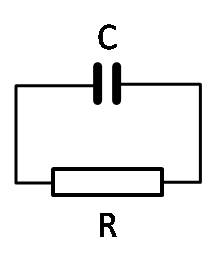
\includegraphics[width=.1\textwidth]{Versuch_15-16/Abbildungen/RC-Kreis.jpg}
	\caption{R-C-Kreis}
	\label{fig:RC-Kreis}
\end{figure}
Die Spannung am Kondensator ($U_C$) ergibt sich aus Gleichung (\ref{eq:I_C}), die Spannung am Widerstand aus der Definition
\begin{equation}
 U_R = R\, I_R\; .
\end{equation}
Nach der Maschenregel muss die Summe aller Ströme in der Masche Null sein. Mit $I = I_C = I_R$ folgt:
\begin{equation}
 U_C + U_R = \frac{1}{C}\int{I\, dt} + R I = 0\; .
\end{equation}
Durch Ableitung nach der Zeit erhält man eine Differentialgleichung für den Strom als Funktion der Zeit:
\begin{equation}
 \frac{dI}{dt} + \frac{1}{RC}\,I = 0\; .
\end{equation}
Diese Differentialgleichung wird gelöst durch die Funktion
\begin{equation}
 I(t) = I_0\, e^{-t/RC}
 \label{eq:Entladekurve}
\end{equation}
Beim Entladen entwickelt sich ein exponentiell mit der Zeit abklingender Strom (ebenso beim Aufladen). Das Produkt $RC$ im Exponenten von Gleichung (\ref{eq:Entladekurve}) bestimmt quantitativ die Abnahme des Stromes und wird als Zeitkonstante bezeichnet.\\

Betrachten wir nun den Wechselstromwiderstand des Kondensators.\\
Mit einer Wechselspannung der Form $U(t) =  U_0\cos\omega t$ finden wir den Strom durch den Kondensator gemäß Gleichung (\ref{eq:I_C}). Mit der Definition des Wechselstromwiderstandes (Gleichung (\ref{eq:Z}) ) berechnet man die Impedanz des Kondensators zu:
\begin{equation}
 Z_C = \frac{U_0}{I_0} = \frac{1}{\omega\, C}\; .
\end{equation}
Ursache des Widerstandes ist die sich aufbauende Gegenspannung am Kondensator. Die dabei umgesetzte Energie bleibt jedoch als elektrische Feldenergie im Kondensator gespeichert und wird während der Entladephase an den Kreis zurückgegeben. Ein (idealer) Kondensator setzt dem Strom einen Widerstand entgegen, der ohne Energieabgabe nach außen bleibt und deshalb als Blindwiderstand bezeichnet wird.\\

Wegen der Frequenzabhängigkeit des Wechselstromwiderstandes von Kondensatoren (und von Spulen) können mit diesen Bauteilen sogenannte Filter gebaut werden, die aus einem Wechselspannungsspektrum bestimmte Frequenzbereiche heraussieben. Solche Filter werden oft benötigt, um in elektrischen Mess- und Steuerkreisen die interessierenden Signale auszuwählen und Störsignale mit anderen Frequenzen abzutrennen. \\
Ein einfaches Beispiel ist die Reihenschaltung eines Kondensators mit einem Widerstand als Spannungsteiler:
\begin{figure}[ht]
	\centering
		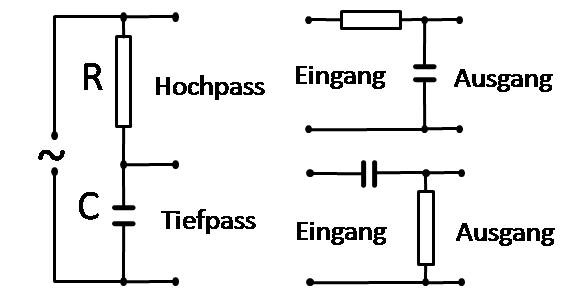
\includegraphics[width=0.5\textwidth]{Versuch_15-16/Abbildungen/Paesse_gross.jpg}
	\caption{Hoch- und Tiefpassschaltungen}
	\label{fig:Hoch-Tiefpass}
\end{figure}
Eine Teilspannung ist proportional dem Teilwiderstand, über dem sie abgegriffen wird. Für tiefe Frequenzen ist der Widerstand des Kondensators groß, so dass hier der Hauptanteil der Eingangsspannung abfällt. Der Abgriff über dem Kondensator stellt einen \textit{Tiefpass} dar. Für hohe Frequenzen ist umgekehrt der Widerstand des Kondensators klein und der des Widerstandes vergleichsweise groß, so dass der Abgriff über dem Widerstand als \textit{Hochpass} wirkt.
%------------------------------------------------
\section{Fragen zur Vorbereitung}
%------------------------------------------------

\begin{enumerate}
 %
 \item Was soll heute im Praktikum untersucht werden? 
 %
 \item Was ist eine Wechselspannung? Wie kann man sie mathematisch beschreiben (Beispiel)? 
 %
 \item Was versteht man unter der Schwingungsdauer/Periode einer Wechselspannung? Wie lautet der Zusammenhang zwischen Periode und Frequenz?
 %
 \item Was versteht man unter einer Effektivspannung/einem Effektivstrom? Wie lautet der entsprechende Zusammenhang für eine sinusförmige Wechselspannung?
 %
 \item Was ist ein Kondensator? Wie sieht ein Plattenkondensator aus?
 %
 \item Was ist die Kapazität eines Kondensators? Wie hängt sie mit Ladung und Spannung zusammen?
 %
 \item Beschreiben Sie anhand einer kleinen Skizze (Spannung in Abhängigkeit der Zeit) die Auf- und die Entladung eines Kondensators über einen ohmschen Widerstand! Wie hängt die Auf-/Entladung des Kondensators von der Größe des Widerstandes ab?
 %
% \item Was ist eine Braun'sche Röhre (Skizze und kurze Erklärung)? Stichworte: Wie wird der Elektronenstrahl erzeugt? Wie wird er abgelenkt?
 %
 \item Wozu dient ein Oszillograph?
 %
 \item Was ist eine Kippspannung? Wozu wird sie im Oszillograph gebraucht? Was wäre auf dem Bildschirm eines Oszillographen zu sehen, wenn man nur eine Wechselspannung anlegt, aber keine Kippspannung?
 %
 \item Wie stellt man eine Wechselspannung auf einem Oszillograph dar? (Stichwort: Überlagerung von zu messender Wechselspannung und Kippspannung)
 %
 \item Wozu dient der Trigger? Stichworte: Was sind Trigger-Level und Triggerflanke?
 %
\end{enumerate}

%------------------------------------------------
\section{Durchführung} 
%------------------------------------------------

\begin{enumerate}
 %
 \item In diesem ersten Versuchsteil sollen Sie sich mit dem Oszilloskop vertraut machen. Stellen Sie eine sinusförmige Wechselspannung auf dem Bildschirm des Oszilloskops dar und beobachten die Abbildung bei verschiedenen Einstellungen des Oszilloskops.\\
  (Anmerkung: In diesem Versuchsteil werden keine für die Auswertung relevanten Messungen durchgeführt.)\\
  
  \noindent
  %Einschalten des Oszilloskops (1), Regeln von Helligkeit (18) und Schärfe (20). Man vergewissere sich, dass folgende Schalter im oberen Bedienungsfeld die richtige Position haben (sie werden nicht 
  %gebraucht!): TV Set: off; Delay: off; Hold-off: rechter Anschlag; Trig: AT.\\
	Man wähle den größten Messbereich für die Eingangsspannung (2). Man verbinde den Eingang des Oszilloskops mit dem Ausgang des Netzgeräts mit Hilfe des Anschlusskabels und einer Massenleitung. Man
	verändere die Zeitauflösung (3) und den Trigger-Level (4) und beobachte das Bild auf dem Bildschirm. Man ändere die Polarität der Triggerflanke (Trig Menu). Man ändere die Ablenkempfindlichkeit (2). Überzeugen Sie sich davon, dass eine Änderung der Ablenkempfindlichkeit bzw. der Zeitauflösung zwar die Auflösung ändert, nicht aber die Spannungsamplitude (in Volt) bzw. die Periode (in Sekunden) der Wechselspannung.
 %
 \item Messen Sie mit Hilfe des Vielfachmessgerätes die Werte der Widerstände $R_C$ und $R_L$ in der Versuchsbox ''Wechselspannungsversuch''. Dazu verbinden Sie die Ausgänge des Vielfachmessgerätes mit 
 	den Anschlussbuchsen ober- und unterhalb des Widerstandes $R_C$ (bzw. $R_L$). Legen Sie keine äußere Spannung an! Diese verfälscht die Messung und kann das Vielfachmessgerät beschädigen.\\
  Bitte notieren Sie die Nummer der Versuchsbox. Anmerkung: Der Widerstand $R_L$ (und die Nummer der Versuchsbox dienen lediglich dem Assistenten als Referenz und werden in der Auswertung nicht 
  benötigt).
 %
	
	\begin{figure}[t]
		\centering
			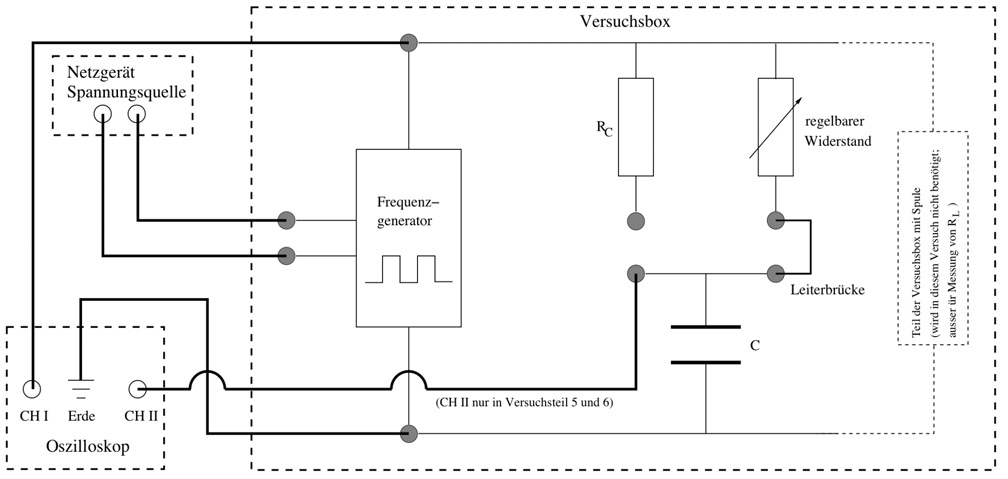
\includegraphics[width=\textwidth]{Versuch_15-16/Abbildungen/Schaltung.jpg}
		\caption{Schaltskizze für den weiteren Versuchsverlauf.}
		\label{fig:Schaltung}
	\end{figure}
	
 \item Verbinden Sie das Netzteil mit dem Eingang des Frequenzgenerators. \\
	\begin{minipage}{0.45\textwidth}
		Verbinden Sie das Oszilloskop mit dem Ausgang des Frequenzgenerators. Die Ausgangsspannung des Frequenzgenerators wird auf dem Bildschirm dargestellt (siehe Abbildung \ref{fig:Schaltung}). Messen Sie die Maximalamplitude 
		$U_0$ sowie die Schwingungsdauer und die Frequenz des Ausgangssignals. Schätzen Sie jeweils Ihre Ablesefehler ab.
	\end{minipage} 
	\hfill
	%
	\begin{minipage}{0.45\textwidth}
		\raggedright
			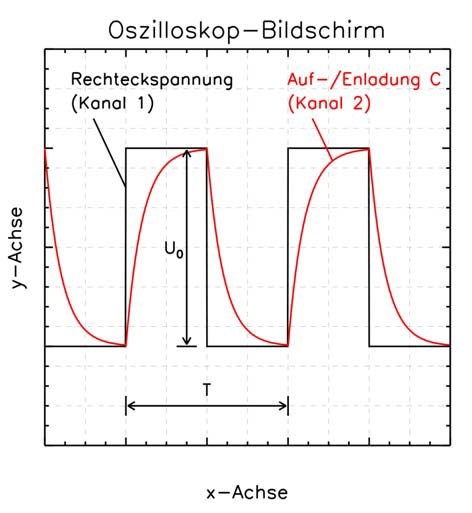
\includegraphics[width=0.7\textwidth]{Versuch_15-16/Abbildungen/Oszi.jpg}
			\label{fig:Oszi}
	\end{minipage}
 %
 \item Auf- und Entladung eines Kondensators über einen Widerstand:\\
	Verbinden Sie den regelbaren Widerstand über die Leiterbrücke mit dem Kondensator. Messen Sie nun mit dem zweiten Kanal des Oszilloskops den Spannungsabfall am Kondensator. Dazu schalten Sie den
	zweiten Kanal am Oszilloskop zu (1). Wählen Sie für beide Eingänge des Oszilloskops die gleiche Empfindlichkeit und bringen Sie die Nulllinien der beiden Eingänge im unteren Bildbereich auf eine Linie. Beachten Sie, dass Sie dazu nur ein Massekabel benötigen (bei korrekter Schaltung)!\\
	Verändern Sie den regelbaren Widerstand und beobachten Sie die Veränderung der Auf- und Entladekurve des Kondensators. Notieren Sie kurz - in Stichworten - Ihre Beobachtung (in der Auswertung ausführlich formulieren)!
 %
 \item Messung der Kapazität eines Kondensators mit dem Oszilloskop:\\
	Verbinden Sie nun den Festwiderstand mit dem Kondensator. Bringen Sie die Aufladungskurve des Kondensators mit bestmöglicher Zeitauflösung auf den Bildschirm und messen Sie die Spannung am 	Kondensator als Funktion der Zeit. Legen Sie dazu eine Folie (liegt im Praktikum aus) über den Bildschirm und pausen sie den Kurvenverlauf ab. (Skalen und Einstellungen mit aufschreiben !!)\\
	Ebenso messe man die Entladung des Kondensators (dazu Triggerflanke (Trig Menu) ändern!). Kann man sich durch geschicktes Drehen/Spiegeln der Folie ggf. ein weiteres 
	Abpausen der Entladekurve sparen? Bitte begründen Sie Ihre Antwort.
 %
 \item Hochpass-Charakteristik des R-L-Kreises:\\
  Entfernen Sie die Leiterbrücke zwischen $R_C$ und dem Kondensator und verbinden stattdessen $R_L$ mit der Spule. Betrachten und skizzieren Sie den Verlauf der Spannung über der Spule. 
 %
\end{enumerate}

%------------------------------------------------
\section{Auswertung} 
%------------------------------------------------

\begin{enumerate}
 %
 \item Beschreiben Sie den Einfluss verschiedener Widerstände bei der Auf- und Entladung eines Kondensators über einen Widerstand (R-C-Kreis).Beachten Sie dabei den Zusammenhang $\tau = R\,C$ und ggf. die Ladung auf dem Kondensator.
 %
 \item Bestimmung der Kapazität $C$ des Kondensators:
  \begin{enumerate}
   %
   \item Übertragen Sie den Kurvenverlauf der Aufladung des Kondensators auf Millimeterpapier. Einheiten und Achsenbeschriftung nicht vergessen!
   %
   \item Für die Aufladung eines Kondensators gilt:
    \begin{equation}
     U_C(t) = U_0\, \left(1-e^{-t/\tau}\right), \quad \tau = R\, C
    \end{equation}
		Lösen Sie diese Gleichung nach $e^{-t/\tau}$ auf und berechnen Sie den natürlichen Logarithmus. Schreiben Sie die neue Gleichung hin. Berechnen Sie die Unsicherheit des Logarithmus.
	 %
   \item Tragen Sie $\ln\left(1-U_C(t)/U_0\right)$ gegen $t$ auf. 
   %
   \item Bestimmen Sie aus der Steigung der Geraden die Kapazität $C$ des Kondensators inklusive Fehler.
   %
  \end{enumerate}
 %
 \item Erläutern Sie kurz, warum man einen R-L-Kreis auch Hochpass nennt.
 %
\end{enumerate}	% Wechselstrom und RC Kreis
\chapter{Spule und Transformator}
\label{v:16}

In diesem Versuch lernen Sie einige Eigenschaften von Spulen und Transformatoren kennen.

%------------------------------------------------
\section{Stichworte}
%------------------------------------------------

Lorentzkraft; Induktionsgesetz; magnetischer Fluss; Selbstinduktion; Effektivwerte für $U$ und $I$; Wechselstromwiderstände; unbelasteter und belasteter Transformator; Spannungsübersetzungsverhältnis.
%
%------------------------------------------------
\section{Literatur}
%------------------------------------------------

Gehrtsen, Kapitel 7.2.3, 7.3.2/5, 7.5.8
%
%------------------------------------------------
\section{Anwendungsbeispiele}
%------------------------------------------------

Unser heutiges Leben wird so sehr von elektrischen Geräten bestimmt, dass man von der ''Elektrozeit'' sprechen könnte. Elektrischer Strom wird meist in Generatoren hergestellt, die mechanische Drehbewegungen (Wasserturbinen, Dampfturbinen, Windräder) ausnutzen, um eine Spule im Magnetfeld zu drehen. Dabei wirkt das Induktionsgesetz. Es bedeutet in Worten, dass jede zeitliche Änderung des magnetischen Flusses eine elektrische Spannung induziert. Es zeigt den Zusammenhang zwischen dem elektrischen und dem magnetischen Feld, wenn beide sich zeitlich verändern und ist von größter Bedeutung in der Elektrotechnik.\\
Die zweite wichtige Anwendung des Induktionsgesetzes ist der Transformator. Er spielt bei der Stromversorgung eine wichtige Rolle, da durch die Hochspannungstransformation (\unit{110}{\kilo}{\volt} bis \unit{380}{\kilo}{\volt}) die Stromstärken für den Transport verringert werden können und somit nach $P = I^2 R$ geringere Verlustleistungen auftreten. ''Tausende'' kleiner Transformatoren umgeben uns überall, um die Wechselspannung von \unit{220}{\volt} aus dem Netz auf die 6 - 12\,V Gleichspannung herunter zu transformieren (bei zusätzlicher Gleichrichtung), die von unseren elektronischen Helfern benötigt werden. Diese kleinen Trafos sind immer warm oder heiß und verbrauchen ständig elektrische Leistung, wenn sie mit dem Netz verbunden sind.\\
Im Versuch wird ein einfacher Transformator untersucht. Es wird versucht, den Begriff der Phase bei Wechselspannungen näher zu bringen.

%------------------------------------------------
\section{Theoretischer Hintergrund}
%------------------------------------------------


\subsection{Transformator}

Ein Transformator betseht aus zwei Spulen, die so angeordnet sind, daß das bei Stromfluß in einer Spule entstehende magnetische Feld die Windungsfläche der anderen Spule durchsetzt und umgekehrt. Jede zeitliche Änderung des Stroms in einer Spule induziert in der anderen - und natürlich in sich selbst - eine Spannung.\\
Man kann daher Leistung von einem mit der Primärspule verbundenen Stromkreis auf einen mit der Sekundärspule verbundenen Kreis übertragen, ohne daß beide Kreise galvanisch (d.h. leitend) miteinander verbunden sind. Häufig wickelt man beide Spulen auf einen (z.B. ringförmig geschlossenen) Eisenkern, um zu erreichen, daß alle magnetischen Feldlinien die Windungsflächen beider Spulen durchsetzen. Die jeweiligen magnetischen Flüße $\Phi_{m,i}$ (i=1,2) und damit die induzierten Spannungen verhalten sich wie die Windungszahlen der Spulen. \\

\noindent
\begin{minipage}{0.6\textwidth}
In der Abbildung rechts sind die beiden Spulen (Windungszahlen $N_1$ und $N_2$) auf ein geschlossenes Eisenjoch gewickelt. An die Primärspule legen wir die Wechselspannung $U_1$ an. Die Sekundärspule schliessen wir mit einer Impedanz Z ab. In der Primärspule fließt ein sinusförmiger, gegen $U_1$ phasenverschobener Strom $I_1$, der wiederum einen zeitlich veränderlichen magnetischen Fluß $\Phi_{m,1}$ hervorruft. Der alternierende magnetische Fluß induziert in der Sekundärspule eine Wechselspannung
\begin{equation}
U_{ind} = -L_1\frac{dI_1}{dt} = -N_1\frac{d\Phi_{m,1}}{dt}\; .
\end{equation}
\end{minipage}
%
\begin{minipage}{0.4\textwidth}
	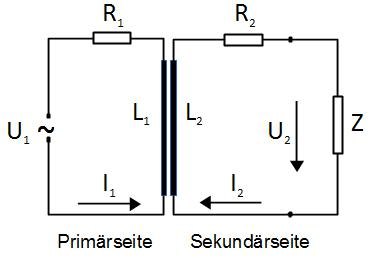
\includegraphics[width=\textwidth]{Versuch_15-16/Abbildungen/Trafo1.jpg}
	\label{fig:Trafo1}
\end{minipage}
%

\noindent
Diese ist nach den Kirchhoff'schen Regeln der von außen angelegten Spannung entgegengesetzt gleich. Wenn der gesamte in der Primärspule erzeugte magnetische Fluß auch durch die Sekundärspule $L_2$ geht, wird dort eine Spannung
\begin{equation}
U_2 = -N_2\frac{d\Phi_{m,1}}{dt}
\end{equation}
induziert. Durch Z und die Spule fließt daraufhin ein Wechselstrom $I_2$. Auch dieser trägt zur Magnetisierung des Kerns bei und veranlaßt eine Rückwirkung des Sekundärkreises auf den Primärkreis (Gegeninduktion).\\
An jeder Spule liegen daher zwei induzierte Spannungen, die den zeitlichen Ableitungen der magnetischen Teilflüsse und damit den zeitlichen Ableitungen der sie erregenden Ströme $I_1$ bzw. $I_2$ proportional sind. Mit den in der Abbildung angegebenen Richtungen, den Induktivitäten von Primär- und Sekundärspule $L_1$und $L_2$, der Gegeninduktivität (mutual inductivity) der beiden Spulen $M$ und den zu den Spulen in Reihe geschalteten Widerständen $R_1$, $R_2$ erhält man die Transformatorgleichungen
\begin{align*}
U_1 & = (i\omega L_1 + R_1) I_1 + i\omega M I_2 &\\
U_2 & = i\omega M I_1 + (i\omega L_2 + R_2) I_2 \; .
\end{align*}

Die Induktivitäten $L_1$, $L_2$ sind proportional zu den Quadraten der Windungszahlen $N_1$, $N_2$ von Primär- und Sekundärspule. Für die Gegeninduktivität gilt $M\propto N_1N_2$. Wenn der gesamte magnetische Fluß beide Spulen durchsetzt gilt weiterhin: $M^2 = L_1L_2$\; . Im Folgenden wollen wir einen verlustlosen Transformator betrachten: $R_1 = R_2 = 0$\; .\\
Für einen \textit{unbelasteten Transformator} ($R = \infty$) findet man dann für die Spannungsübersetzung:
\begin{equation} \label{eq:Spannungsuebersetzung}
\frac{U_2}{U_1} = \frac{M}{L_1} = \frac{N_2}{N_1}\; .
\end{equation}

\noindent
Für die Stromübersetzung im Kurzschlußfall findet man:
\begin{equation} \label{eq:Stromuebersetzung}
\frac{I_2}{I_1} = \frac{M}{L_2} = \frac{N_1}{N_2}
\end{equation}
%------------------------------------------------
\section{Fragen zur Vorbereitung}
%------------------------------------------------

\begin{enumerate}
	%
	\item Was ist eine Wechselspannung/ein Wechselstrom? Wie kann man sie/ihn mathematisch beschreiben (Beispiel)?
	%
	\item Was versteht man unter einer Effektivspannung/ einem Effektivstrom? Wie lautet der entsprechende Zusammenhang für eine sinusförmige Wechselspannung?
	%
	\item Was versteht man unter elektrischer Leistung? Was gilt für die mittlere elektrische Leistung in einem Wechselstromkreis? (Stichwort: Phasenverschiebung zwischen Strom und Spannung)
	%
	\item Wie lautet der Zusammenhang zwischen Strom und Spannung für einen ohmschen Widerstand in einem Wechselstromkreis?
	%
	\item Wie lautet der Zusammenhang zwischen Strom und Spannung für den kapazitiven Widerstand eines idealen Kondensators in einem Wechselstromkreis?
	%
	\item Wie lautet der Zusammenhang zwischen Strom und Spannung für den induktiven Widerstand einer idealen Spule in einem Wechselstromkreis?
	%
	\item Wie lautet der Zusammenhang für den Gesamtwiderstand (Impedanz) einer Reihenschaltung von ohmschen, kapazitiven und induktiven Widerstand in einem Wechselstromkreis?
	%
	\item Was haben das Magnetfeld eines Stabmagneten und das einer Spule gemeinsam? Wie sieht der Verlauf der Feldlinien aus?
	%
	\item Wie verlaufen die Magnetfeldlinien im Inneren einer langen Spule? Welcher Zusammenhang gilt zwischen magnetischer Flussdichte B und Stromstärke I (keine detaillierte Formel, nur proportional, quadratisch, reziprok o.ä.)?
	%
	\item Was ist die Lorentzkraft? Wie ist sie definiert?
	%
	\item Was besagt das Induktionsgesetz? Welche Bedeutung hat das Minuszeichen (Stichwort: Lenzsche Regel)?
	%
	\item Was ist ein Transformator? Wie ist er aufgebaut? Welche Aufgabe hat der Eisenkern?
	%
	\item Wozu dient ein Transformator?
	%
	\item Was versteht man unter einem unbelasteten Transformator? Was versteht man unter einem belasteten Transformator? (Hilfe: Schaltskizze)
	%
	\item Wie leitet sich das Spannungsübersetzungsverhältnis $\frac{U_1}{U_2}=\frac{N_1}{N_2}$ bzw. das Stromübersetzungsverhältnis $\frac{N_1}{N_2}=\frac{I_2}{I_1}$ beim Transformator ab ?
 %
\end{enumerate}

%------------------------------------------------
\section{Durchführung} 
%------------------------------------------------

\begin{enumerate}
	%
	\item \label{VT1}
	%\textit{Der Folgende Versuchsteil wird durch den Assistenten durchgeführt:}\\
		\textbf{Phasenverschiebung an einer Spule:}\\
		Man schließe den Schiebewiderstand in Reihe mit der Primärspule (Spule 1 = Sp1) des Transformators und verbinde sie direkt mit dem Ausgang des Netzgerätes. Man stelle die Spannung an der Spule und die Spannung am Ausgang des 
		Netzgerätes auf dem Oszilloskop dar.\\
		
		\begin{figure}[h]
			\centering
				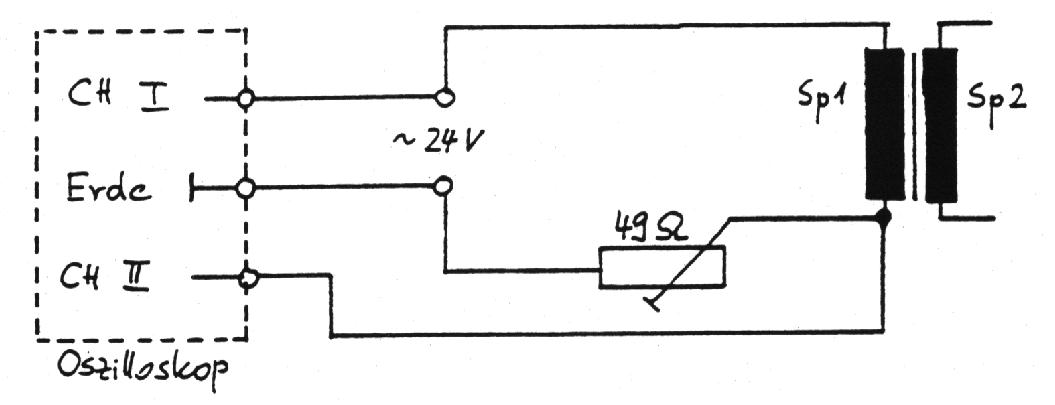
\includegraphics[width=0.50\textwidth]{Versuch_15-16/Abbildungen/Bild31.jpg}
			\label{fig:Bild31}
		\end{figure}
		
		Dazu verbinde man Kanal 1 (CH I) mit einem Pol des Netzgeräts, den anderen Pol mit der Erde des Oszilloskops. Kanal 2 (CH II) wird mit der Spule gemäss Schaltbild verbunden. Das Wechselspannungs-Netzgerät wird auf 25\% 
		der Leistung reduziert. Man messe (qualitativ) die Phasenverschiebung zwischen den beiden Signalen! Beträgt die Phasenverschiebung 0°, 90° oder liegt sie dazwischen?
	%
	\item \textbf{Unbelasteter Transformator:}\\ 
		Man benutze Spule 1 als Primärspule und Spule 2 als Sekundärspule.\\
		\begin{minipage}{0.55\textwidth}
			Messen Sie die Sekundärspannung $U_2$ in Abhängigkeit der Primärspannung $U_1$. Variieren Sie dazu $U_1$ in Schritten von 3\,V im Bereich $0\leq U_1\leq 24$\,V.\\
			\textit{Hinweis: Die Spannungsangaben in der Zeichnung stellen die empfohlenen Messbereiche der Voltmeter dar.}
		\end{minipage}
		%
		\begin{minipage}{0.45\textwidth}
			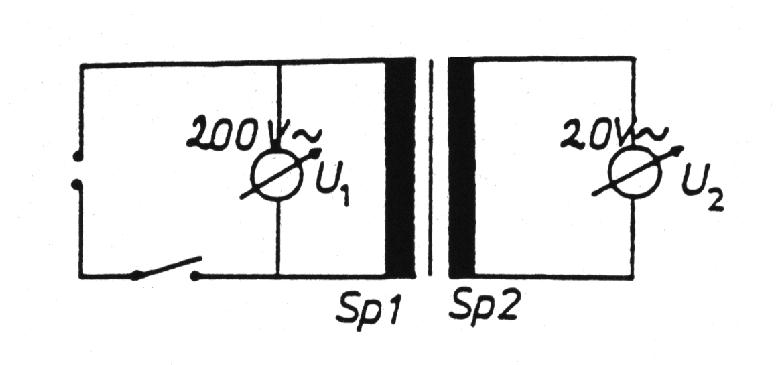
\includegraphics[width=\textwidth]{Versuch_15-16/Abbildungen/BILD20.jpg}
			\label{fig:Bild20}
		\end{minipage}
	%
	\item \textbf{Belasteter Transformator:}\\
	Bevor Sie mit diesem Versuchsteil beginnen, lesen Sie bitte die gesamte Anleitung, inklusive des unten stehenden Kastens, aufmerksam durch. Bei diesem Versuchsteil können Sie ansonsten gehörigen Schaden an den Geräten anrichten!\\
	
	\noindent
	Legen Sie an die Primärspule 1 eine Spannung $U_{eff}$\,=\,20\,V und bauen Sie in den Sekundärkreis einen ohmschen Widerstand ein.\\
		\begin{minipage}{0.55\textwidth}
			Messen Sie den Strom auf der Primärseite $I_1$ in Abhängigkeit des Stroms auf der Sekundärseite $I_2$. Variieren Sie dazu $I_2$ in Schritten von 0,2\,A im Bereich $0\leq I_2\leq 2$\,A.\\
		\end{minipage}
		%
		\begin{minipage}{0.45\textwidth}
			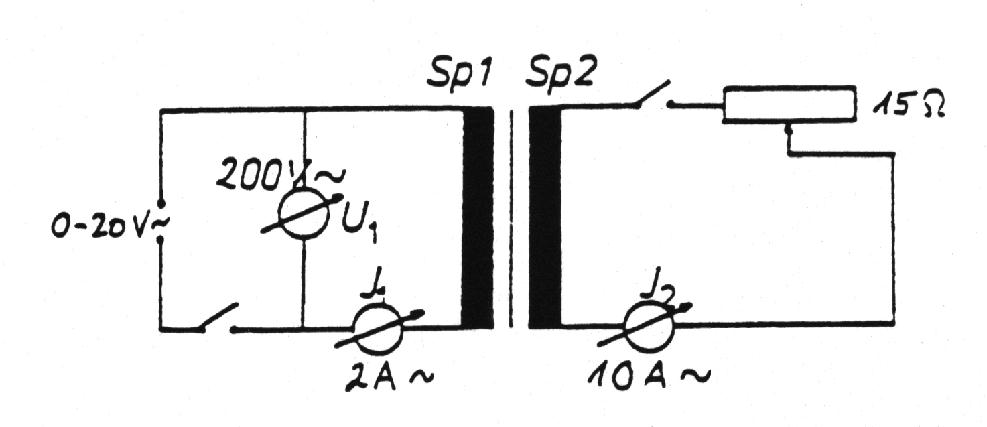
\includegraphics[width=\textwidth]{Versuch_15-16/Abbildungen/BILD22.jpg}
			\label{fig:Bild22}
		\end{minipage}
		
	\begin{important}
	\begin{enumerate}[label={\roman*}.]
		%
		\item Achten Sie darauf, dass die Spannung im Primärkreis während des gesamten Versuchs bei konstant $U_1$\,=\,20\,V liegt! Regeln Sie ggf. nach!
		%
		\item Vorsicht bei der Regulierung der Stromstärke $I_2$ durch Verschieben des regelbaren Widerstandes. Die Stromstärke ändert sich nicht linear mit der Verschiebung des Widerstandes. D.h. bei kleinen Stromstärken $I_2$ 
			führen kleine Verschiebungen zu kleinen Änderungen von $I_2$, bei großen Stromstärken führen kleine Verschiebungen des Widerstandes zu großen Änderungen der Stromstärke $I_2$.\\
			\textbf{Messgeräte nicht überlasten!}
		%
	\end{enumerate}
	\end{important}
\end{enumerate}

%------------------------------------------------
\section{Auswertung} 
%------------------------------------------------

\begin{enumerate}
%
\item Erklären Sie kurz den Begriff ''Phasenverschiebung'' am Beispiel von Versuchsteil \ref{VT1}.. Warum ist die dort beobachtete Phasenverschiebung kleiner als 90\degree?
%
\item Stellen Sie die Messreihe $U_2\,=\,f(U_1)$ graphisch dar! Bestimmen Sie aus der Steigung der Auftragung das Spannungsübersetzungsverhältnis $U_2/U_1$.

	\noindent
	\textbf{Bemerkung:} Es kann vorkommen, dass ''so gut'' gemessen wurde, dass alle Messwerte auf einer Geraden liegen, so dass sich keine ''sinnvollen'' Fehlergeraden einzeichnen lassen. Bestimmen Sie in diesem Fall (und nur in
	diesem Fall!!!) das Spannungsübersetzungsverhältnis als Mittelwert mit Standardabweichung aus den Einzelmessungen des Spannungsübersetzungsverhältnisses $U_2/U_1$! D.h. berechnen Sie die einzelnen Verhältnisse und dann den Mittelwert daraus. \\
	Eine korrekte Fehlerrechnung wird für den weiteren Teil der Auswertung benötigt!
%
\item Stellen Sie die Messreihe $I_1\,=\,f(I_2)$ graphisch dar! Bestimmen Sie aus der Steigung der Auftragung das Stromübersetzungsverhältnis $I_1/I_2$ (mit Fehler)!

	\noindent
	\textbf{Bemerkung:} Obwohl man annimmt, dass $I_1/I_2\, =\,N_2/N_1$ gilt, ergibt die graphische Auftragung keine Gerade. Das liegt daran, dass bei der Herleitung des o.g. Zusammenhangs stark idealisiert wurde!
%
\item Die Windungszahl der Sekundärspule beträgt $N_2\,=\,72$. Bestimmen Sie anhand der Beziehungen $U_2/U_1\,=\,N_2/N_1$ für den unbelasteten Transformator und $I_1/I_2\,=\,N_2/N_1$ für den belasteten Transformator jeweils die Windungszahl $N_1$ der Primärspule inklusive ihres Fehlers.
%
\item Berechnen Sie anhand der beiden Einzelergebnisse für $N_1$ den gewichteten Mittelwert von $N_1$ (mit Fehler des gewichteten Mittelwerts)!
%
\end{enumerate}	% Spule und Transformator

\chapter{Drehschwingungen}
\label{v:2}

In diesem Versuch lernen Sie die Grundlagen der Rotation starrer (nicht verformbarer) Körper kennen.
% Zusätzlich: Schwingen mit angezogenen Armen beim Laufen, um Rotationsenergie zu reduzieren,
% Pirouette beim Eiskunstlauf
% --> Haben wir einen Probekörper an einer langen Achse?
% --> Drehmoment in die Anleitung?
%------------------------------------------------
\section{Stichworte}
%------------------------------------------------
Lineare (harmonische) Schwingungen; Drehschwingungen; Winkelgeschwindigkeit; Drehimpulserhaltung; Trägheitsmoment; Drehmoment; Steinerscher Satz; 
%
%------------------------------------------------
\section{Literatur}
%------------------------------------------------
Gehrtsen, Kapitel 1.4.2/3, 2.1 und 2.2; Demtröder, Kapitel 2.4.1, 2.8, 4.5, 5.5
%
%------------------------------------------------
\section{Anwendungsbeispiele}
%------------------------------------------------
%
Die Rotation starrer Körper und die dabei verwendeten Trägheitsmomente der Körper beschreiben nicht nur die Vorgänge bei der Rotation eines Spielzeugkreisels oder des Gyroskopstabilisators von Schiffen, sondern auch die Rotation von Atomen und Molekülen, bei denen manche Achsen (Hauptträgheitsachsen) bevorzugt sind. Die Rotation der Erde um ihre eigene Achse wird ebenso beschrieben wie die Umdrehung von Fahrradreifen oder die Rotation des Arms in der Schulter.
%
%------------------------------------------------
\section{Theoretischer Hintergrund}
%------------------------------------------------

\subsection{Das Trägheitsmoment}

Wir betrachten einen starren Körper, der um eine feststehende Achse rotiert. Um die gesamte kinetische Energie des Körpers aufgrund seiner Rotation berechnen zu können, unterteilen wir den Körper in sehr kleine würfelförmige Elemente, die die kleine Masse $dm_i$ (\textit{Massenelement}) haben. Diese Massenelemente haben den senkrechten Abstand $r_i$ von der Drehachse. Somit können wir die gesamte kinetische Energie schreiben als:
\begin{equation}
\label{Gl:Erot_sum}
E_{rot} = \frac{1}{2} \sum{dm_i v_i^2} = \frac{1}{2} \omega^2 \sum{dm_i r_i^2}
\end{equation}
mit der Winkelgeschwindigkeit $\omega = r\cdot v$.\\
Bei einem kontinuierlichen Körper können wir das Massenelement $dm_i$ über die Dichte des Körpers ausdrücken als $dm_i = \rho\cdot dV$. Lassen wir nun die Würfel, aus denen wir den Körper zusammensetzen, unendlich klein (infinitesimal) werden, so geht die Summe in Gleichung \ref{Gl:Erot_sum} in das Integral über:
\begin{equation}
\label{Gl:Erot_integral}
E_{rot} = \frac{1}{2}\omega^2\int{\rho r^2 dV}
\end{equation}
%
Wir lassen die Dichte $\rho$ unter dem Integral, weil sie von Ort zu Ort verschieden sein kann. \\

Betrachten wir den in Gleichung \ref{Gl:Erot_integral} auftretenden Ausdruck
\begin{equation}
\label{Gl:Traegheitsmoment}
J = \sum{dm_i r_i^2} = \int{\rho r_i^2 dV} \; ,
\end{equation}
das \textit{Trägheitsmoment} des Körpers. Er besagt, dass sich die einzelnen Masseteile in der Rotation umso mehr auswirken, je weiter sie von der Rotationsachse entfernt sind. Dementsprechend hängt $J$ sowohl von der genauen Form des Körpers ab, als auch davon, wo die Rotationsachse des Körpers liegt. Beispielsweise betragen die Trägheitsmoment einiger einfacher Körper:
\begin{itemize}
\item Kreisscheibe oder Zylinder, Achse durch die Symmetrieachse:
	\begin{equation} \label{eq:J_Zylinder}
	J = \frac{1}{2} MR^2
	\end{equation}
\item Hohlzylinder (Innenradius $R_i$, Aussenradius $R_a$), Achse durch Symmetrieachse:
	\begin{equation}
	J = \frac{1}{2} M(R_a^2 + R_i^2)
	\end{equation}
\item Vollkugel, Achse durchs Zentrum:
	\begin{equation}
	J = \frac{2}{5} MR^2
	\end{equation}
\item Würfel der Kantenlänge $a$, für jede Achse, die durch den Schwerpunkt geht:
	\begin{equation}
	J = \frac{1}{6} Ma^2
	\end{equation}
\item Stab der Länge $L$, Achse senkrecht zum Stab durch den Schwerpunkt:
	\begin{equation}
	J = \frac{1}{12} ML^2
	\end{equation}
\end{itemize}

\subsection{Der Steiner'sche Satz}

Wenn man das Trägheitsmoment eines Körpers in Bezug auf eine durch seinen Schwerpunkt gehende Achse $A'$ kennt, liefert der \textit{Steiner'sche Satz} das Trägheitsmoment in Bezug auf eine andere dazu parallele Achse $A$. Der Abstand zwischen den beiden Achsen sei $a$:
\begin{equation}
\label{Gl:Steiner}
J_A = J_{A'} + Ma^2
\end{equation}
%
Wie man leicht nachrechnen kann, ergibt sich damit für das Trägheitsmomentes eines Stabes, bei dem die Drehachse einen Abstand $b$ zum Schwerpunkt hat:
\begin{equation} \label{eq:J_Stab-Steiner}
J = \frac{1}{12}ML^2 + mb^2 \, .
\end{equation}

\subsection{Drehschwingungen}

Eine Spiralfeder übt ein Drehmoment $\vec{T}$ aus, das dem Auslenkungswinkel aus der Ruhelage proportional und entgegengerichtet ist:
\begin{equation}
 \vec{T} = -D^*\cdot\varphi\cdot \hat{e}_{\varphi} \; .
\end{equation}
$D^*$ heißt \textit{Winkelrichtgröße} oder \textit{Richtmoment} und ist eine Eigenschaft der gewählten Feder. Unter der Wirkung eines solchen Moments führt ein an der Spiralfeder befestigter Körper entsprechend der Bewegungsgleichung
\begin{equation}
 \vec{T} = -D^*\cdot\varphi\cdot \hat{e}_{\varphi} = \dot{\vec{L}} = J\ddot{\varphi}\cdot\hat{e}_{\varphi}
\end{equation}
Drehschwingungen aus. Das Symbol $\dot{\vec{L}}$ bezeichnet dabei die zeitliche Änderung des Dreh- impulses $\vec{L} = m\cdot \vec{r}\times\vec{p}$. Analog zu den Translationsschwingungen aus Versuch 1 ergibt sich für die Frequenz der Schwingung:
\begin{equation}
 \omega = \frac{2\pi}{T} = \sqrt{\frac{D^*}{J}}
\end{equation}
$T$ ist hierbei die Schwingungsdauer.

%------------------------------------------------
\section{Fragen zur Vorbereitung}
%------------------------------------------------

\begin{enumerate} 
 %
% \item Was soll heute im Praktikum gemessen werden? Warum?
 %
 \item Welche Gr"o{\ss}en beschreiben eine Drehbewegung?
 %
 \item Wie lautet der Steiner'sche Satz?
 %
 \item Was ist eine harmonische Schwingung?
 %
 \item Gilt die Energie-Erhaltung bei der Spiralfeder? Beschreiben Sie die Energieverhältnisse während der Drehschwingung.
 %
 \item Wie ist das Drehmoment definiert? (Formel und Einheit)
 % 
 \item Wie ist der Drehimpuls definiert? (Formel und Einheit)
 %
\end{enumerate} 

%------------------------------------------------
\section{Durchführung} 
%------------------------------------------------

\begin{enumerate}
 %
 \item Der Halter wird so eingespannt, dass die Drehachse horizontal liegt. An der aufgesteckten Scheibe wird die Schnur befestigt. Für verschiedene an die Schnur gehängte Massen (m = 10, 15, 20, 30, 40~g) wird der Winkelausschlag $\Phi$ im Uhrzeigersinn und entgegengesetzt abgelesen. Achten Sie darauf, dass die Feder nicht an den Rahmen anschlägt!
 %
 \item Messen Sie den Radius $r$ der Scheibe.
 %
 \item Tragen Sie für jede Masse $M$ den entsprechenden Winkelausschlag $\Phi$ im Bogenma{\ss} auf. Bilden Sie dazu jeweils den Mittelwert aus der Auslenkung im und gegen den Uhrzeigersinn und bestimmen Sie die Fehler auf diese Mittelwerte.
 %
 \item Messen Sie bei vertikaler Lage der Drillachse für jeden Versuchskörper dreimal die Zeit für jeweils 10 Drehschwingungen. Beim Würfel sind zwei verschiedene Drehachsen zu wählen. Beim Stab werden zwei parallele Achsen gewählt; eine davon geht durch den Schwerpunkt, die andere liegt am Ende des Stabes.
 %
 \item Messen Sie die geometrischen Daten der Versuchskörper (Radien, Kantenlängen). Die Masse $M$ der Versuchskörper ist jeweils auf den Körpern in Gramm angegeben.
 %
\end{enumerate}

%------------------------------------------------
\section{Auswertung} 
%------------------------------------------------

\begin{enumerate}
 %
 \item Berechnen Sie aus der Steigung der Funktion $\Phi (M)$ das Richtmoment (Winkelrichtgröße) $D^*$ der Feder nach der Formel:
 \begin{equation}
 D^* = \frac{M}{\Phi}\cdot g\cdot r \; .
 \end{equation}
 Berechnen Sie auch den Fehler auf das Richtmoment.
 %
 \item Berechnen Sie die Trägheitsmomente $J_{exp}$ der verschiedenen Versuchskörper aus den gemessenen Schwingungsdauern $T$. Benutzen Sie:
 \begin{equation}
 T = 2\pi\sqrt{\frac{J_{exp}}{D^*}} \; .
 \end{equation}
 Fehlerrechnung nicht vergessen!
 %
 \item Berechnen Sie aus den geometrischen Daten der Versuchskörper die theoretischen Trägheitsmomente $J_{th}$ inklusive ihrer Fehler. Benutzen Sie die Gleichungen \ref{eq:J_Zylinder} bis \ref{eq:J_Stab-Steiner}.
 %
 \item Vergleichen Sie die gemessenen und berechneten Werte $J_{exp}$ und $J_{th}$ für die verschiedenen Versuchskörper. Geben Sie eine Erklärung für mögliche Differenzen zwischen den Werten.
 %
\end{enumerate}			% Drehschwingungen --> Tr�gheitsmoment
\chapter{Freie gedämpfte Schwingungen}
\label{vn:1}

In diesem Versuch werden die Grundlagen der freien und der angeregten Schwingung mit Dämpfung anhand des Pohl'schen Resonators untersucht.

%\noindent
%{\bf Kenntnisse}: ???

%------------------------------------------------
\section{Stichworte}
%------------------------------------------------
Pohl'scher Resonator, Schwingungsgleichung, harmonische Schwingung, Resonanz, Dämpfung.
%
%------------------------------------------------
\section{Literatur}
%------------------------------------------------
Gehrtsen, Kapitel 2.1-2.4, 4.2; Demtröder, Kapitel 5.1-5.6, 11.1-11.5; Walcher, Kapitel 2.7.4
%
%------------------------------------------------
\section{Anwendungsbeispiele}
%------------------------------------------------
%
Bewegungsabläufe lassen sich darin unterscheiden, ob sie sich regelmäßig wiederholen oder nicht. Als periodische Vorgänge bezeichnet man Prozessen, bei denen sich jeder Zustand des Systems immer nach derselben Zeitdauer wiederholt. Nicht-periodische Vorgänge sind Abläufe, die nur einmal auftreten oder sich unregelmäßig wiederholen (z. B. der Aufprall von Regentropfen).\\
Schwingungen und Wellen sind periodische Strukturen, deren Verständnis grundlegend für sämtliche naturwissenschaftliche Bereiche ist. Eine Schaukel, die Stimmlippen in Ihrem Kehlkopf, ein elektrischer Schwingkreis schwingen. In der pharmazeutischen Industrie finden Schwingungen Anwendung bei Vibrationssieben und -filtern, in der Medizin stellen Ultraschallschwingungen ein wichtiges nicht-invasives Diagnosewerkzeug zur Verfügung, sogar die Populationsentwicklung biologischer Arten kann unter bestimmten Umständen durch Schwingungen beschrieben werden.\\
Da Ihnen also Schwingungen in allen möglichen Themen-/Arbeits-/Forschungsgebieten begegnen, wollen wir uns hier, wenn auch nur oberflächlich, mit ihren wichtigsten mathematischen Eigenschaften und den daraus resultierenden Phänomenen beschäftigen.
%
%------------------------------------------------
\section{Theoretischer Hintergrund}
%------------------------------------------------

\subsection{Freie Schwingung mit Dämpfung}

Bewegt sich ein Körper in eine Richtung $x$ während eine Rückstellkraft auf ihn wirkt, die der Bewegungsrichtung entgegengesetzt und proportional zu $x$ ist, so stellt sich eine Schwingung ein. Die Bewegung des  Körpers wird mit wachsendem $x$ immer stärker gebremst, bis er zum Stillstand kommt und sich danach in $-x$~Richtung zurückbewegt. Wenn er die Ausgangslage überschreitet wiederholt sich derselbe Vorgang. Diesen periodisch wiederkehrenden Vorgang nennt man \textit{Schwingung}, die Zeit $T$, die verstreicht, bis sich ein Bewegungszustand (bestimmt durch Ort, Betrag und Richtung der Geschwindigkeit) wieder einstellt, heißt \textit{Schwingungsdauer}. Die \textit{Frequenz} einer Schwingung ist definiert durch
\begin{equation}
f = 1/T \; ,
\end{equation}
ihre \textit{Kreisfrequenz} $\omega$, auch Winkelfrequenz genannt, durch
\begin{equation}
\omega = 2\pi f = 2\pi /T\; .
\end{equation}
%
Ist die rücktreibende Kraft linear proportional zu $x$, so handelt es sich um eine \textit{harmonische Schwingung}. Diese Art von ungedämpften, freien Schwingungen haben Sie im Vorversuch \ref{v:0} und in der Vorlesung kennengelernt.\\
Eine Schwingung, deren Amplitude durch Energieverlust monoton abnimmt, heißt \textit{gedämpfte Schwingung}. Im einfachsten Fall rührt der Energieverlust von Reibung oder einer anderen Kraft her, die proportional zur Geschwindigkeit des Körpers $v = \frac{{\rm d} x}{\rm dt} = \dot{x}$ ist. Eine rücktreibende Kraft, die proportional zu $x$ ist, kann zum Beispiel von einer Feder mit der Federkonstanten $D$ ausgeübt werden. Damit ergibt sich die Bewegungsgleichung des Körpers zu
\begin{equation}
	m\ddot{x} + b\dot{x} + Dx = 0 \, .
\label{eq:Schwingungsgleichung_vn1}
\end{equation}

Der im Versuch benutzte Aufbau nach Pohl, der \textit{Pohl'sche Resonator}, funktioniert genauso wie die oben beschriebene lineare Schwingung, wobei Rückstellkraft und Reibung aus einer Drehbewegung resultieren, sodass anstelle der linearen Auslenkung $x$ der Auslenkungswinkel $\varphi$ betrachtet wird. Auf die Drehscheibe mit dem Trägheitsmoment $\Theta$ wirkt durch die Spiralfeder ein zu $\varphi$ proportionales Rückstellmoment $D^*\varphi$. Die Wirbelstrombremse (und natürlich auch Reibung) erzeugen ein bremsendes Moment $\rho\dot{\varphi}$, welches proportional zur Winkelgeschwindigkeit ist. Damit erhalten wir die Bewegungsgleichung des Pohl'schen Resonators:
\begin{equation}
	\Theta\ddot{\varphi} + \rho\dot{\varphi} + D^*\varphi = 0\, .
\end{equation}
%
Bringen wir diese Differenzialgleichung auf die Normalform, indem wir durch $\Theta$ teilen, erhalten wir mit den Definitionen $2\beta := \rho /\Theta$ und $\omega_0^2 := D^* /\Theta$ eine homogene Differenzialgleichung 2. Ordnung:
\begin{equation}
	\ddot{\varphi} + 2\beta\dot{\varphi} + \omega_0^2 \varphi = 0 \, .
\label{eq:Bewegungsgleichung_Pohl}
\end{equation}
%
Setzt man den Ansatz $\varphi (t)= A \exp(\lambda t)$ in Gleichung \ref{eq:Bewegungsgleichung_Pohl} ein, so findet man (im Allgemeinen) zwei Werte für $\lambda$:
\begin{equation*}
	\lambda_{1,2} = -\beta \pm \sqrt{\beta^2 - \omega_0^2}\, .
\end{equation*}
%
Es sind drei Fälle zu unterscheiden, die drei charakteristische Bewegungsformen beschreiben:
\begin{enumerate}[label=\alph*.)] 
	\item \textbf{Kriechfall}: $\beta^2 > \omega_0^2$\\
		Man findet, dass $\gamma := \sqrt{\beta^2 - \omega_0^2} > 0$ und eine reelle Zahl ist. Damit sind die beiden Werte von $\lambda$ negative reelle Zahlen und die allgemeine Lösung der Schwingungsgleichung
		\begin{equation*}
			\varphi(t) = A\exp((-\beta+\gamma) t) + B\exp((-\beta -\gamma) t)
		\end{equation*}
		Die Konstanten $A$ und $B$ sind dabei durch die Anfangsbedingungen gegeben.\\
		Die Dämpfung ist sehr stark, so dass es nicht zu einer Schwingung kommt. Der Körper kehrt langsam, ohne Überschwinger, zur Ausgangslage ($\varphi = 0$) zurück.
	%
	\item \textbf{Aperiodischer Grenzfall}: $\beta^2 = \omega_0^2$\\
		Man findet (mit etwas weiterem Rechnen) für die Lösung der Schwingungsgleichung
		\begin{equation*}
			\varphi(t) = \varphi_0\left(1 + \omega_0 t\right) \exp(-\omega_0 t)\, .
		\end{equation*}
		Wieder ist der Exponent eine reelle Zahl, so dass auch diese Lösung keine Schwingung darstellt.\\
		Die Reibung ist so stark, dass das System gerade so nicht schwingt, sondern in besonders kurzer Zeit in die Ruhelage zurückkehrt.
	%
	\item \textbf{Schwingfall}: $\beta^2 < \omega_0^2$\\
		In diesem Fall findet man für $\lambda$ zwei verschiedene, komplexe Werte:
		\begin{equation*}
			\lambda_{1,2} = -\beta \pm i\sqrt{\omega_0^2 - \beta^2}
		\end{equation*}
		Mit den Anfangsbedingungen findet man dann für die Lösung der Schwingungsgleichung den Ausdruck
		\begin{equation}
			\varphi(t) = \varphi_0\exp(-\beta t)\cdot\cos(\hat{\omega}t) \quad \mathrm{mit}\quad \hat{\omega}=\sqrt{\omega_0^2 -\beta^2}\, .
			\label{eq:Schwingfall}
		\end{equation}
		Wie man sieht ist die Eigenfrequenz $\hat{\omega}$ dieser gedämpften Schwingung kleiner als die der ungedämpften Schwingung.\\
		Die Amplitude
		\begin{equation}
			\varphi(t) = \varphi_0\cdot \exp(-\beta t)
			\label{eq:Amplitude_gedaempft}
		\end{equation}
		klingt exponentiell ab.
		
\end{enumerate}

\begin{figure}[ht!]
\begin{center}
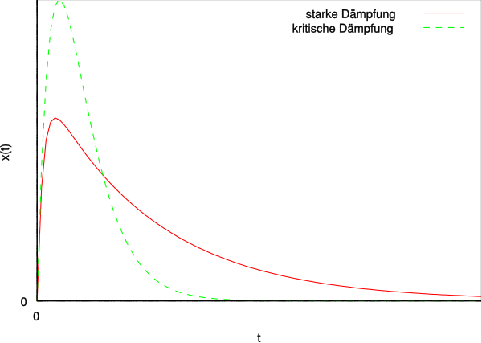
\includegraphics[width=0.45\textwidth]{Versuch_neu_1-2/figures/2285.pdf}
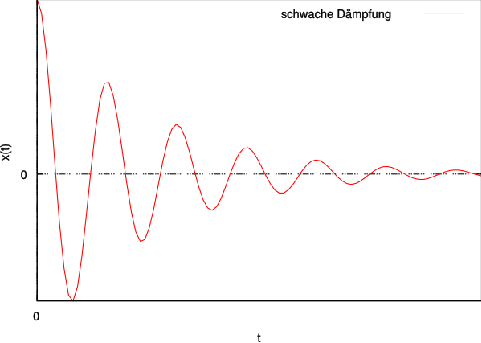
\includegraphics[width=0.45\textwidth]{Versuch_neu_1-2/figures/2284.pdf}
\end{center}
\caption{Zeitlicher Verlauf der Amplitude einer Schwingung im Kriechfall und aperiodischen Grenzfall (links) und im gedämpften Schwingfall (rechts).}
\label{fig:Schwingungen}
\end{figure}

\subsection{Angeregte Schwingung mit Dämpfung}

Wirkt auf das schwingungsfähige System das äußere periodische Anregungsmoment $M\cos(\omega t)$, so wird die Bewegungsgleichung eine inhomogene lineare Differentialgleichung 2. Ordnung. Diese kann man zwar analytisch lösen, was wir hier aber dem ''geneigten Leser'' überlassen wollen.\\
Nach dem Einschwingvorgang, währenddessen die Bewegung des Systems eine Überlagerung der Bewegung mit seiner Eigenfrequenz $\omega_0$ sowie einer mit der Erregerfrequenz $\omega$ ist, lautet die Lösung der Bewegungsgleichung 
\begin{equation}
	\varphi(t) = \frac{N}{\sqrt{\left(\omega_0^2 - \omega^2\right)^2 +4\beta^2\omega^2}}\cos(\omega t - \alpha)\, .
\end{equation}
Dies ist eine Schwingung mit der Frequenz $\omega_e$, welche um den Winkel $\alpha$ gegen die Phase der Erregerschwingung verschoben ist. \\
Wie man sieht, ist die Amplitude 
\begin{equation*}
	\varphi_0 = \frac{N}{\sqrt{\left(\omega_0^2 - \omega^2\right)^2 +4\beta^2\omega^2}}
\end{equation*}
abhängig von der Differenz der Erregerfrequenz zur Eigenfrequenz des Systems $\left(\omega_0^2 - \omega^2\right)^2$ und zur Dämpfung $\beta$. Sie wird maximal, wenn die Erregerfrequenz der \textit{Resonanzfrequenz} entspricht, die sich ergibt als:
\begin{equation}
	\omega_r = \sqrt{\omega_0^2 -2\beta^2}\, .
\end{equation}

\begin{figure}[ht!]
	\centering
	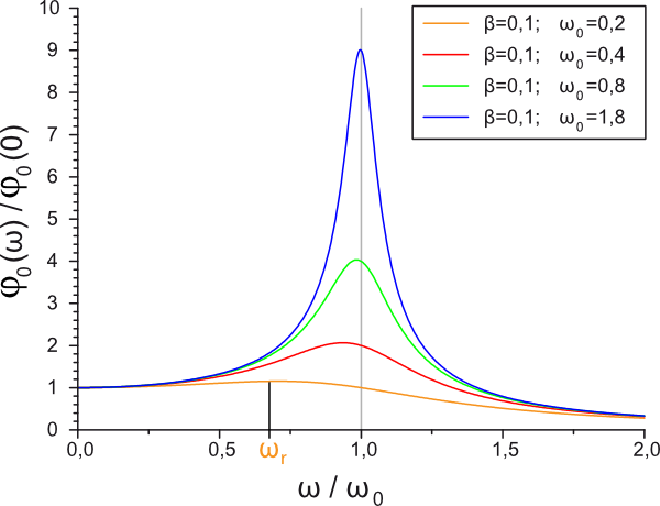
\includegraphics[width=0.45\textwidth]{Versuch_neu_1-2/figures/3946.pdf}
	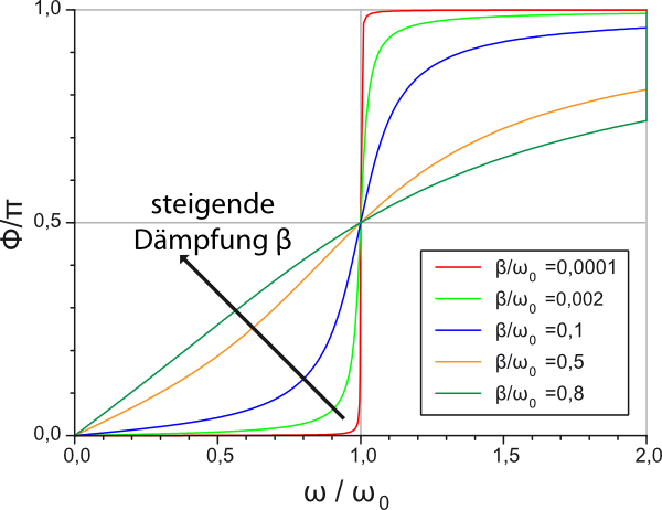
\includegraphics[width=0.45\textwidth]{Versuch_neu_1-2/figures/3947.pdf}
	\caption{Links: Frequenzgang einer angeregten, gedämpften Schwingung für verschiedene Dämpfungen. Beachten Sie die Verschiebung der Resonanzfrequenz. Rechts: Phasenverschiebung einer angeregten, gedämpften Schwingung für verschiedene Dämpfungen.}
	\label{fig:Resonanz}
\end{figure}

Auch die Phasenverschiebung hängt von der Differenz der Erreger- und Eigenfrequenz und der Dämpfung ab:
\begin{equation*}
	\tan\alpha = \frac{2\beta\omega}{\omega_0^2-\omega^2}
\end{equation*}
Wie in Abbildung \ref{fig:Resonanz} zu sehen ist, ist die Phasenverschiebung (für genügend kleine Dämpfung) sehr klein bei Frequenzen kleiner als der Eigenfrequenz des Systems, das System folgt dem Erreger sehr genau. Überschreitet die Erregerfrequenz die Eigenfrequenz, so wird die Phasenverschiebung 90\degree, das System eilt dem Erreger um eine halbe Schwingung hinterher.
%------------------------------------------------
\section{Fragen zur Vorbereitung}
%------------------------------------------------

\begin{enumerate} 
	\item Skizzieren Sie von Hand die Funktion $f(t) = \cos(\omega t)$. Welche Werte nimmt diese an für $\omega t = 0\, , \pi/2\, , \pi\, , 3\pi/4\, , 2\pi$?
	%
	\item Unter welchen Bedingungen tritt eine resonant angeregte Schwingung auf? Wie verhält sich die Amplitude der Schwingung in diesem Fall?
	%
	\item Was ist der konzeptionelle Unterschied zwischen der Frequenz $f$ und der Kreisfrequenz $\omega$?
	%
	\item Wieso ist die detaillierte Kenntnis der Eigenschwingungsfrequenzen von Gebäuden, Brücken oder den Flügeln eines Flugzeuges wichtig?
	%
	\item Beschreiben Sie die Bewegung eines gedämpften, schwingfähigen Systems im Schwingfall, Kriechfall und im aperiodischen Grenzfall? Wann tritt welcher der drei Fälle ein?
\end{enumerate} 

%------------------------------------------------
\section{Durchführung} 
%------------------------------------------------

\subsection{Vorbereitung}

Starten Sie den PC und melden Sie sich als Benutzer »Prakt« (kein Passwort) an. Schalten Sie die Motorsteuerung in dem separaten Kasten auf der Rückseite ein. Starten Sie das Programm »Pohl« über die Verknüpfung auf dem Desktop. Ihre Messdaten werden nach dem Ende jeder einzelnen Messung graphisch dargestellt und sollten umgehend ausgedruckt werden. Zusätzlich wird eine PDF-Datei in dem angegebenen Verzeichnis gespeichert. Bitte nicht in anderen Verzeichnissen Dateien verändern oder löschen.

\subsection{Bedienung des Messprogramms}

Das Programm »Pohl« ist eine grafische Oberfläche für die Messwertaufnahme am Pohlschen Resonator.
\begin{enumerate}
	\item Starten Sie das Programm »Pohl«, falls dies noch nicht geschehen ist.
	%
	\item Legen Sie eine neue Messung an. Geben Sie hierzu die Parameter der Messung in den dafür vorgesehen Textfeldern an, damit diese im Ergebnisgraphen vermerkt werden. Die Frequenz geben Sie bitte in Millihertz (mHz) an, mit der der Exzenter betrieben werden soll. Ein Wert von 250 lässt den Exzenter also in 4 Sekunden eine vollständige Umdrehung durchführen. Bei der Eingabe von 0 ist der Exzenter deaktiviert.
	%
	\item Klicken Sie auf den Button »neue Messung starten«, um eine neue Messreihe anzulegen. Die Datenaufnahme und ggf. auch die Motorsteuerung starten nun.
	%
	\item Das Pohlsche Rad befindet sich nun in Eigenschwingung bzw. im Einschwingvorgang. Dabei wird der Amplitudenverlauf grafisch aufgetragen, sobald das Rad zwecks Kalibrierung der Auslese die Nulllage zwei mal durchlaufen hat (vorher keine Datenanzeige). 
	%
	\item Bei der erzwungenen Schwingung empfiehlt es sich, sobald der Einschwingvorgang beendet ist, die Messung durch einen Klick auf den Button »Messreihe neu starten« erneut zu starten. Bei Messung der Eigenschwingung empfiehlt es sich, gerade bei starker Dämpfung, zunächst die Initialisierung der Elektronik abzuwarten, dann das Rad erneut auszulenken und den Button »Messreihe neu starten« zu betätigen.
	%
	\item Durch einen Klick auf die Reiter »Amplitude« bzw. »Phasenraum« können Sie sich verschiedene Messdaten schon während der Messung anschauen.
	%
	\item Wenn Sie genug Daten haben, beenden Sie die Messung mit einem Klick auf »Messung beenden«. Es wird nachfolgend eine PDF-Datei mit dem graphisch dargestellten Ergebnis angelegt und angezeigt; diese bitte umgehend ausdrucken.
\end{enumerate}

\subsection{Durchführung}

\begin{enumerate}
	% Messung der Eigenfrequenz des Resonators bei Dämpfung 0 --> ablese aus Plot
	\item Bringen Sie den Motor mit dem Messprogramm in Position 0.
	%Messung des Amplitudenverlaufs für verschieden starke Dämpfung --> nur Betrachten?
	\item Starten Sie die Messung für die freie Schwingung für vier verschiedene Stellungen des Millimetertriebs der Wirbelstrombremse: 0, 4, 6 und 8~mm. Die Skala des Millimetertriebs weist dabei ggf. einen Versatz auf: »0 mm« bezieht sich auf die Position bei Deckung der Kante des Magneten mit der Außenseite des Kupferrads und die anderen Angaben gelten relativ dazu. Regen Sie den Resonator bei abgeschaltetem Motor zu Eigenschwingungen an (Anregung 0~Hz; falls nötig die Nulllage des Motors vorher per Software einstellen). Dabei die Auslenkung der Drehscheibe von Hand auf 120° stellen und loslassen. Während einer kurzen Initialisierungsphase der Messelektronik werden noch keine Messdaten angezeigt.
	%
	\item Messen Sie nun bitte die erzwungene gedämpfte Schwingung. Für drei verschiedene Dämpfungen 4, 6 und 8~mm (Stellung am Millimetertrieb der Wirbelstrombremse) führen Sie dazu jeweils die nachfolgenden Schritte durch:
	\begin{enumerate}
		\item Nehmen Sie für die jeweils eingestellte Dämpfung für genügend viele verschiedene Frequenzen (150-600~mHz) die Schwingung des Oszillators auf. Stellen Sie sicher, dass 
		der Einschwingvorgang vorbei ist, bevor Sie die Datenaufzeichnung starten. Hierbei muss die Amplitude des Pohl'schen Resonators zeitlich konstant sein. Achten Sie weiterhin darauf, dass genügend viele Schwingungen aufgezeichnet werden.
		%
		\item Machen Sie insbesondere in der Nähe der Resonanz viele Messungen. Achten Sie dabei jedoch auf eine mögliche Resonanzkatastrophe. In diesem Fall ist die Messung sofort über »Messung beenden« zu beenden.
	\end{enumerate}
\end{enumerate}
Für die Auswertung sind die ausgedruckten Graphen ausreichend. Wer es vorzieht, die PDF-Dateien zu verwenden, sollte diese über das Internet oder einen mitgebrachten USB-Stick übertragen. Am einfachsten geht dies mit einer E-Mail an sich selbst. Ihr/e Betreuer/in kann Ihnen dabei helfen.

%------------------------------------------------
\section{Auswertung} 
%------------------------------------------------

\begin{enumerate}
	%
	\item \label{aw:Schwingfall} Lesen Sie aus den zeitlichen Verläufen der vier verschieden gedämpften Schwingungen deren jeweilige Frequenz $\hat{\omega}$ ab.
	%
	\item \label{aw:Log_Dekrement}Tragen Sie für die vier verschieden gedämpften Schwingungen den Logarithmus der maximalen Auslenkung, $\ln\varphi(t)$ s. Gl. \ref{eq:Amplitude_gedaempft}, als Funktion der Zeit auf. Diesen finden Sie für die Halbwelle mit positiver Auslenkung auf der zweiten Seite des zur Messung gehörenden pdf-Dokumentes. \\
	Lesen Sie aus dem Graphen die Dämpfung $\beta$ inkl. ihrer Unsicherheit ab.
	%
	\item Berechnen Sie mit Hilfe von Gleichung \ref{eq:Schwingfall} für jede der vier verschieden gedämpften Schwingungen jeweils $\omega_0$. Mitteln Sie über diese vier Werte, um die Eigenfrequenz des ungedämpften Systems inklusive ihrer Unsicherheit zu berechnen.
	%
	\item Bestimmen Sie die Amplitude der angeregten Schwingungen für die verschiedenen Erregerfrequenzen aus den zugehörigen Graphen. Mitteln Sie graphisch über mehrere Perioden, indem Sie jeweils eine Gerade parallel zur x-Achse  an die maximalen Amplituden der positiven Halbwellen anpassen. 
	%
	\item Tragen Sie nun das Verhältnis der Amplitude bei der jeweiligen Erregerfrequenz zur Amplitude bei einer Frequenz nahe Null, $\varphi(\omega)/\varphi(0)$, als Funktion des Verhältnisses der Erregerfrequenz zur Eigenfrequenz des ungedämpften Systems, $\omega/\omega_0$, auf. Dabei sollen die Kurven für die verschiedenen Dämpfungen in denselben Graphen eingetragen werden.
\end{enumerate}	% Pohl'scher Resonator

\chapter{Kapillarität und Auftrieb}
\label{v:3}

In diesem Versuch lernen Sie, wie man die Oberflächenspannung von Flüssigkeiten misst, sowie eine Methode zur Bestimmung der Dichte einer unbekannten Flüssigkeit.

%------------------------------------------------
\section{Stichworte}
%------------------------------------------------
Oberflächenspannung; Kapillarität; Auftrieb; Mohr'sche Waage; Drehmoment.
%
%------------------------------------------------
\section{Literatur}
%------------------------------------------------
Gehrtsen, Kapitel 3.1.4 und 3.2; Walcher, Kapitel 2.3 und 2.5
%
%------------------------------------------------
\section{Anwendungsbeispiele}
%------------------------------------------------
%
Eine Kapillare ist ein sehr feiner, langgestreckter Hohlraum. Das Wort leitet sich vom lateinischen Wort capillus (das Haar) ab.\\
Der Kapillareffekt (oder die Kapillarität) beschreibt das Verhalten einer Flüssigkeit in einer solchen Kapillare, wo die Flüssigkeit aufgrund der Oberflächenspannung an den Wänden der Kapillare ''hinaufkriecht''. Der Effekt wird zum Beispiel von Pflanzen benutzt, um Wasser von den Wurzeln, entgegen der Schwerkraft, zu den Blättern zu transportieren. In der Papierchromatographie wird eine Lösung auf Spezialpapier getropft, wo sie aufgrund der Kapillarität aufsteigt und Bestandteile der Lösung mit sich trägt. Aufgrund der Laufweiten können die Stoffe getrennt werden. Auch in Gesteinen treten Kapillareffekte auf, die Wasser durch das Gestein bewegen.
%
%------------------------------------------------
\section{Theoretischer Hintergrund}
%------------------------------------------------

\subsection{Dichtemessung}

Die Dichte eines homogenen Körpers der Masse $M$ und des Volumens $V$ ist definiert als das Verhältnis
\begin{equation} \label{eq:Dichte}
 \rho = \frac{M}{V} \; .
\end{equation}

Die Masse eines Körpers läßt sich im Allgemeinen durch Wiegen sehr genau ermitteln. Das Volumen eines unregelmäßig geformten Körpers ist hingegen nicht einfach direkt zu bestimmen. Zur mittelbaren Bestimmung des Volumens eignet sich in vielen Fällen der Auftrieb $F_A$, den ein Körper erfährt, wenn man ihn in eine Flüssigkeit der Dichte $\rho_{Fl}$ taucht. Die Auftriebskraft ist gegeben durch
\begin{equation} \label{eq:Auftrieb}
 F_A = g\cdot \rho_{Fl}\cdot V\, .
\end{equation}

Andererseits ist die Auftriebskraft gegeben durch die Differenz der Gewichtskraft $F_g^L$, die der Körper in Luft erfährt, und der Gewichtskraft $F_g^{Fl}$, die er in der Flüssigkeit erfährt:
\begin{equation} \label{eq:Gew-Diff}
 F_A = F_g^L - F_g^{Fl} \; .
\end{equation}

Mithilfe der obigen Gleichungen findet man nun einen Ausdruck für die Dichte des Körpers:
\begin{equation} \label{eq:rho}
 \rho = \rho_{Fl}\frac{F_g^L}{F_g^L - F_g^{Fl}} \; .
\end{equation}

\subsection{Die Mohr'sche Waage}

Mißt man die Dichte eines Probekörpers zweimal nacheinander in verschiedenen Flüssigkeiten, so sind in Gleichung \ref{eq:rho} die beiden Gößen $\rho$ und $F_g^L$ konstant. Für das Verhältnis der Dichten (die \textit{relative Dichte}) ergibt sich
\begin{equation} \label{eq:rel_Dichte}
 \frac{\rho_{Fl,1}}{\rho_{Fl,2}} = \frac{F_A^{Fl,1}}{F_A^{Fl,2}} \; .
\end{equation}

Die Gewichtskräfte, die auf den Probekörper in den beiden Flüssigkeiten wirken, bestimmt man mit der Mohr'schen Waage. \\
Hierbei wird der Probekörper in Luft an die Waage gehängt, und diese über das verschiebbare Eichgewicht wieder ins Gleichgewicht gebracht. Wird der Probekörper nun in Flüssigkeit getaucht, so übt die Auftriebskraft ein Drehmoment auf den Arm der Waage aus, welches diesen nach oben drückt. Durch Auflegen der gebogenen Gewichte in die verschiedenen Positionen des Waagenarms lässt sich das Gleichgewicht wiederherstellen.\\
Damit ergibt sich:
\begin{equation}
 \rho_{Fl,1} = \rho_{Fl,2}\frac{\sum_{i=1}^n{m_i^{Fl,1}\cdot r_i}}{\sum_{j=1}^n{m_j^{Fl,2}\cdot r_j}}
\end{equation}

\subsection{Oberflächenspannung und Kapillarität}

Zwischen den Molekülen einer Flüssigkeit wirken die van~der~Waals-Kräfte. Die effektive Reichweite der van~der~Waals-Kräfte ist so klein ($F\sim r^{-6}$), daß auf ein bestimmtes Molekül in der Flüssigkeit nur die nächsten Nachbarn Kräfte ausüben. Im Inneren der Flüssigkeit sind die Moleküle homogen verteilt, sodass auf ein bestimmtes Molekül in alle Richtungen die gleiche Kraft wirkt. Diese heben sich damit auf. Die Moleküle an der Oberfläche der Flüssigkeit haben nun in einer Richtung (aus der Flüssigkeitsoberfläche hinaus) keine Nachbarn, sodass sich eine nach Innen gerichtete Gesamtkraft ergibt. Diese Kraft führt dazu, dass die Oberfläche einer Flüssigkeit dazu tendiert, eine Kugelform einzunehmen (s. Seifenblase).

Taucht man nun eine Kapillare vom Durchmesser $2r$ in eine Flüssigkeit der Dichte $\rho$, so dass sie ganz von der Flüssigkeit benetzt ist, so steigt diese in der Kapillare bis zu einer Höhe $h$ hoch. Die Flüssigkeitssäule hat die Gewichtskraft
\begin{equation}
 F_g = \rho\, V\, g = \rho\,\pi\, r^2\, h\, g
\end{equation}
und hängt an einer ringförmigen Lamelle, die die Kraft
\begin{equation}
 F_s = \sigma\, 2\,\pi\, r
\end{equation}
überträgt. Damit folgt für die Oberflächenspannung:
\begin{equation} \label{eq:Oberflaechenspannung}
 \sigma = \frac{1}{2}\rho\,g\,r\,h\; .
\end{equation}


%------------------------------------------------
\section{Fragen zur Vorbereitung}
%------------------------------------------------

\begin{enumerate} 
 \item Was soll heute im Praktikum gemessen werden? Warum?
 %
 \item Welche Kräfte wirken zwischen Molekülen in einer Flüssigkeit?
 %
 \item Was sind van der Waals-Kräfte?
 %
 \item Wodurch entsteht die Oberflächenspannung?
 %
 \item Warum erfährt ein Körper in einer Flüssigkeit Auftrieb?
 %
 \item Wie lautet das Archimedische Prinzip?
 %
 \item Warum ragt ein Eisberg aus dem Wasser?
 %
 \item Wie funktioniert die Mohr'sche Waage?
\end{enumerate} 

%------------------------------------------------
\section{Durchführung} 
%------------------------------------------------

Zu Beginn werden von der Versuchsgruppe drei verschiedene Kapillaren ausgewählt. Die Kapillare sind mit einem farbigen Rand versehen (Rot, Blau, Grün) - jede Gruppe benötigt jeweils alle drei Farben.\\

Jede der Kapillaren wird mit der Einrichtung im Raum gesäubert. Dazu gehören alle drei Stufen: 1. Lösungsmittel, 2. Weichwasser und 3. Trocknung.

\begin{enumerate}
%
 \item Messen Sie die Kapillarradien mit dem Messmikroskop: \\
 Zuerst wird die Kapillare, mit dem Ausflussende zum Experimentator zeigend, auf das Mikroskop gelegt. Dort wird durch vor-/zurückschieben der Kapillaren ein scharfes Bild eingestellt. Durch den  Schattenwurf der Kapillaren entstehen mehrere Ringe - der innerste ist hier die zu vermessende Öffnung. Das Fadenkreuz wird auf den linken Rand eingestellt und auf der Skala abgelesen. Nun wird auf den rechten Rand der Kapillaren gefahren und wiederum die Skala abgelesen. Es müssen jeweils 5 Werte aufgenommen werden.\\
 Beachten Sie: Da die Kapillaren nicht perfekt rund sind, muss die Kapillare für ein neues Wertepaar leicht gedreht werden.
 %
\end{enumerate}
%
\begin{important}
	Da das Praktikum nur 2 Messapparate bietet, kann man sich zum Beispiel auch schon mal um die nachfolgenden Versuchsteile kümmern.
\end{important}
%
\begin{enumerate} \setcounter{enumi}{1}
 \item Wiegen Sie das leere Auffanggefäß und die Probekörper (jeweils einmal). 
 %
 \item Füllen Sie das Becherglas mit dem schrägen Auslass bis zu dessen Oberkante mit Wasser. Lassen Sie nun den Metallklotz in das Wasser und messen danach die Masse des Wassers im Auffanggefäß. \\
 Füllen Sie das Becherglas erneut bis zur Oberkante und lassen Sie den Holzklotz in das Wasser. Da er nicht komplett untergeht müssen Sie neben der Masse des ausgelaufenen Wassers auch die Eintauchtiefe und die Kantenlänge des Klotzes messen.
 %
\end{enumerate}
%
\begin{important}
	In den nachfolgenden Versuchsteilen (3 \& 4) geht es viel schneller wenn man jeweils die Versuche Steighöhen messen und Mohr'sche Waage hintereinander mit einer Flüssigkeit durchführt.
\end{important}

Hier soll mit drei verschiedenen Flüssigkeiten gemessen werden: Wasser, Äthylenglykol, Methylalkohol. Die letzten beiden befinden sich im Eingangsbereich des Versuchsraums.
%
\begin{enumerate} \setcounter{enumi}{3}
 %
 \item Die Kapillare mit dem mittleren Radius wird tief in die Flüssigkeit getaucht. Damit ist die Innenseite der Kapillaren benetzt. Dann wird sie bis zur unteren schwarzen Markierung an der Kapillaren aus der Flüssigkeit gezogen. Hier ist die Steighöhe (innerhalb der Kapillaren) der Flüssigkeit abzulesen (1 Strich = 1 mm). Danach wird die Kapillare wieder komplett eingetaucht und erneut für eine Messung herausgezogen. Es müssen hier 5 Werte für die Steighöhe für alle 3 Flüssigkeiten bestimmt werden.
 %
 \item Bestimmen Sie die Dichten $\rho_{Fl}$ der drei Flüssigkeiten mithilfe der Mohr'schen Waage:
  \begin{itemize}
   \item Zuerst muss die Waage justiert werden. Dazu wird das Eichgewicht ganz langsam und vorsichtig so geschraubt, dass die Waage mit angehängtem Probekörper wieder im Gleichgewicht ist. 
   \item Danach wird der Probekörper ganz (inkl. Öse) in die zu untersuchende Flüssigkeit getaucht. Beachten Sie dabei, dass der Probekörper nicht an die Wand des Gefäßes stößt.
  \end{itemize}
  Der Körper steigt aufgrund seines Auftriebs nach oben und bringt die Waage aus dem Gleichgewicht. Bringen Sie nun solange mit der Pinzette die gebogenen Gewichte an die verschiedenen Positionen des Waagenarms an, bis die Waage wieder im Gleichgewicht ist. Notieren Sie Lage (in cm) und Masse (in mg) der Gewichte.\\
  
  Beachten Sie, dass der Probekörper zwischen den Messungen mit verschiedenen Flüssigkeiten gründlich getrocknet werden muss. Warum?
 %
\end{enumerate}
%------------------------------------------------
\section{Auswertung} 
%------------------------------------------------

\begin{enumerate}
 %
 \item Bestimmen Sie die mittleren Radien $r_k$ der drei Typen von Kapillaren (blau, rot, grün) inklusive deren Fehler.
 %
 \item Berechnen Sie die Dichte $\rho_M$ des Metallkörpers inklusive Fehler.
 %
 \item Berechnen Sie die Dichte $\rho_H$ des Holzkörpers inklusive Fehler.
 %
 \item Berechnen Sie die Dichten $\rho_{Fl}$ von Äthylenglykol und Methylalkohol inklusive Fehler.
 %
 \item Bestimmen Sie die Oberflächenspannungen $\sigma$ von destilliertem Wasser, Methylalkohol und Äthylenglykol nach Gleichung \ref{eq:Oberflaechenspannung} und bestimmen Sie den Fehler von $\sigma$ aus den statistischen Messfehlern mittels Gauß'scher Fehlerfortpflanzung.
\end{enumerate}			% Kapillarit�t und Auftrieb
\chapter{Innere Reibung von Flüssigkeiten}
\label{v:4}

In diesem Versuch lernen Sie die Grundlagen der Reibung in Flüssigkeiten kennen.

%------------------------------------------------
\section{Stichworte}
%------------------------------------------------

Innere Reibung; dynamische Viskosität; laminare Strömung; Hagen-Poiseuillesches Gesetz.
%
%------------------------------------------------
\section{Literatur}
%------------------------------------------------

Gehrtsen, Kapitel 3.3.2 und 3.3.3; Walcher, Kapitel 2.6.0 und 2.6.1
%
%------------------------------------------------
\section{Anwendungsbeispiele}
%------------------------------------------------
%
Die Viskosität ist ein Maß für die Zähflüssigkeit eines Fluids, je höher die Viskosität, desto zähflüssiger. Die Viskosität spielt in allen Bereichen, wo fließende Flüssigkeiten auftreten eine Rolle:\\
Motorenöl ersetzt die Reibung von Metall auf Metall durch innere Reibung im Öl, mit kleinen Radiusänderungen der Adern erreicht der Körper eine Regelung der Durchflussmenge im Blutkreislauf in weiten Grenzen, das Durchmischungsverhalten von Flüssigkeiten ist sowohl bei Lösungen im Labor, als auch bei der Herstellung von Lacken etc. wichtig.
%
%------------------------------------------------
\section{Theoretischer Hintergrund}
%------------------------------------------------

\subsection{Innere Reibung}

Zwischen einer festen Wand und einer dazu parallelen, bewegten Platte befinde sich eine dünne Flüssigkeitsschicht der Dicke $z$. Um die Platte der Fläche $A$ mit konstanter Geschwindigkeit $\vec{v}$ parallel zur Wand zu verschieben, braucht man eine Kraft
\begin{equation} \label{eq:Kraft}
 \vec{F} = \eta\,A\frac{\vec{v}}{z}\; .
\end{equation}
Die dynamische Viskosität $\eta$ beschreibt die Eigenschaften der Flüssigkeit. Dass in Gleichung \ref{eq:Kraft} $A$ und $\vec{v}$ im Zähler stehen, ist leicht einzusehen. Warum aber steht die Schichtdicke $z$ im Nenner?\\
Hierzu muss man sich klar machen, dass es sich bei der Gegenkraft zu $\vec{F}$ nicht um die Reibung zwischen Festkörper und Flüssigkeit handelt. Das liegt daran, dass die direkt an die Wände angrenzenden Flüssigkeitsschichten an diesen haften. Vielmehr kommt die Gegenkraft durch die Reibung zwischen verschiedenen Schichten in der Flüssigkeit zustande. Zwischen Wand und Platte bildet sich in der Flüssigkeit ein Geschwindigkeitsprofil aus, bei dem die Geschwindigkeit der einzelnen Flüssigkeitsschichten mit wachsendem Abstand von der Wand linear ansteigen. Je kleiner $z$ bei einer gegebenen Geschwindigkeit der Platte ist, desto schneller müssen also die einzelnen Molekülschichten der Flüssigkeit übereinander weggleiten.\\
Die durch die Kraft $\vec{F}$ von aussen zugeführte Energie wird komplett in Wärme umgewandelt. Diesen Zustand der Flüssigkeit nennt man \textit{laminare Strömung}.\\

Steigert man $\vec{v}$, so tritt im Allgemeinen beim Überschreiten eines kritischen Wertes $v_{krit}$ ein weiterer Anteil zur Reibungskraft hinzu: Die Flüssigkeit zwischen Wand und Platte wird in wirbelnde Bewegung versetzt. Die von aussen zugeführte Energie wird nun zum Teil in kinetische Energie der Flüssigkeit umgesetzt. Diesen Zustand nennt man \textit{turbulente Strömung}.\\

Analoge Überlegungen gelten natürlich auch für strömende Flüssigkeiten zwischen ruhenden Wänden, z.B. Blut in Adern, Motoröl, etc.

Die Viskosität von Flüssigkeiten nimmt mit steigender Temperatur sehr stark ab (das Medium wird 'dünn-flüssiger'). Für viele Flüssigkeiten gilt in guter Näherung $\eta = \eta_{\inf}\, e^{b/T}$.

Ist die Viskosität unabhängig von der Geschwindigkeit $v$, so spricht man von eine \textit{Newton'schen Flüssigkeit}. Die meisten reinen Flüssigkeiten sind Newton'sch. Für bestimmte Mischungen hingegen lässt sich die innere Reibung nicht mehr einfach durch das \textit{Newton'sche Reibungsgesetz}, s. Gl. \ref{eq:Kraft}, beschreiben, die Fließeigenschaften ändern sich, wenn zum Beispiel eine äußere Kraft auf die Flüssigkeit einwirkt. Beispiele für solchen nichtnewtonsche oder anomalviskose Flüssigkeiten sind Blut, Zementleime, Treibsand oder Ketchup.

%------------------------------------------------
\section{Fragen zur Vorbereitung}
%------------------------------------------------

\begin{enumerate}
 %
 \item Was soll heute im Praktikum gemessen werden? Warum?
 %
 \item Wie ist der Druck definiert? (Einheiten)
 %
 \item Was heißt hydrostatischer Druck?
 %
 \item Welche Strömungstypen gibt es?
 %
 \item Was ist Viskosität? Wodurch entsteht sie?
 %
 \item Welche Einheit hat die Viskosität?
 %
 \item Wie verhält sich die Viskosität bei steigender Temperatur?
 %
 \item Unter welchen Vorrausetzungen gilt das Hagen-Poiseuillesche Gesetz?
 %
 \item Wie lautet das Hagen-Poiseuillesche Gesetz?
 %
 \item Worauf bezieht sich die Druckdifferenz $\Delta$p im Hagen-Poiseuilleschen Gesetz?
 %
\end{enumerate}

%------------------------------------------------
\section{Durchführung} 
%------------------------------------------------

\begin{enumerate}
 %
 \item Messen Sie die Auslaufzeit $t$ in Sekunden von $h\,=\,45\,$cm auf $h\,=\,35\,$cm für alle drei Kapillaren. Wiederholen Sie die Messung für jede Kapillare dreimal.
 %
 \item Messen Sie für die Kapillare mit mittlerem Durchmesser die Auslaufzeit in Abhängigkeit von der Flüssigkeitshöhe $h$. Notieren Sie dazu bei durchlaufender Stoppuhr jeweils die Zeit, bei der die Flüssigkeitssäule um weitere 5~cm gesunken ist. Messen Sie die Zeit im Intervall zwischen $h\,=\,50\,$cm und $h\,=\,10\,$cm.\\
 Bereiten Sie eine Tabelle wie folgt vor:
 \begin{table}[h]
	\centering
		\begin{tabular}{|c|c|c|c|}
			$h_i$ [m] & $t_i$ [s] & $h_i/h_0$ & ln($h_i/h_0$)\\ \hline \hline
			0,5 & 0 & & \\
		\end{tabular}
 \end{table}
 %
 \item Messen Sie die Länge $l$ der Kapillaren, den Radius $R_V$ des Vorratsbehälters, sowie die Temperatur des (destillierten ?) Wassers.
 %
\end{enumerate}

%------------------------------------------------
\section{Auswertung} 
%------------------------------------------------

\begin{enumerate}
 %
 \item Berechnen Sie den Druckunterschied zwischen der Ober- und Unterseite der Kapillare aus der mittleren Wasserhöhe. Benutzen Sie hierfür
  \begin{equation}
		\Delta p = \rho\cdot g\cdot h_{mittel}\; .  
  \end{equation}
 %
 \item \label{Aufg:Vis1}
 Berechnen Sie die Viskosität $\eta$ von Wasser nach dem Hagen-Poiseuilleschen Gesetz
  \begin{equation} \label{eq:HP}
   \frac{V}{t} = \frac{\Delta p\cdot\pi}{8\eta l}r_k^4
  \end{equation}
 für die drei Kapillaren. Berechnen Sie die Fehler mithilfe der Gaußschen Fehlerfortpfanzung.
 %
 \item Tragen Sie den Logarithmus der relativen Wasserhöhe $\ln(h_i/h_0)$ als Funktion der Auslaufzeit $t$ auf. Bestimmen Sie die Steigung $m$ der Gerade inklusive ihres Fehlers (Anlegen von Grenzgeraden).\\

	\underline{Herleitung:}\\
	Es gilt: $\Delta p(t) = \frac{Kraft}{Flaeche} = \frac{\rho g\cdot h(t) \pi R_V^2}{\pi R_V^2} = \rho g\cdot h(t)$\; .\\
	Damit wird das Hagen-Poiseuillesche Gesetz zu 
	\begin{equation} \label{eq:HP1}
		\frac{dV}{dt} = \frac{\pi r_K^4}{8\eta l}\Delta p(t) = \frac{\rho g\pi r_K^4}{8\eta l} h(t) := C_1\cdot h(t)\; .
	\end{equation}
	Das Flüssigkeitsvolumen im Vorratsbehälter beträgt $dV = \pi R_V^2 dh$, damit wird Gleichung \ref{eq:HP1} zu
	\begin{equation}
		\frac{dh}{dt} = \frac{C_1}{\pi R_V^2} h(t) := C\cdot h(t)\; .
	\end{equation}
	Separation der Variablen ergibt $\frac{dh}{h(t)} = m\cdot dt$.\\
	Integrieren wir diese Formel in den gemessenen Grenzen $\int^{h_1}_{h_0} \frac{dh}{h(t)} = m\int^{t_1}_0 dt$\\
	so ergibt sich
	\begin{equation}
		ln\left(\frac{h_1}{h_0}\right) = m\cdot t_1 = \frac{\rho g r_K^4}{8\eta l R_V^2}\cdot t_1
	\end{equation}
 %
 \item \label{Aufg:Vis2}
 Berechnen Sie aus der Steigung der Geraden die Viskosität $\eta$ nach
  \begin{equation}
   \eta = -\frac{\rho g\,r_K^4}{8\,l\,R^2_V}\frac{1}{m}\; .
  \end{equation}
 Bestimmen Sie den Fehler der Viskosität aus der Gaußschen Fehlerfortpflanzung.
 %
 \item Stimmen die in den Aufgaben \ref{Aufg:Vis1} und \ref{Aufg:Vis2} gemessenen Werte mit dem Literaturwert für die Viskosität mit Wasser überein? Wenn nicht, diskutieren Sie Quellen für Abweichungen vom Literaturwert (z.B.: Welche Annahmen sind gemacht worden?).
\end{enumerate}			% Innere Reibung von Fl�ssigkeiten

\documentclass[11pt, twoside, a4paper]{book}

\usepackage{graphicx}
\usepackage[utf8]{inputenc}
\usepackage{ngerman}
%\usepackage{lineno}
\usepackage{verbatim}
\usepackage[squaren]{SIunits}
\usepackage{amsmath}
\usepackage{amsfonts}
\usepackage{amssymb}
\usepackage{enumitem}
\usepackage{fancyhdr}
\usepackage{textcomp}
\usepackage{subcaption}
\usepackage[noadjust]{marginnote}
\usepackage{tikz}
\usepackage{nicefrac}
\usepackage{framed}
\usepackage{import}

\usetikzlibrary{calc,intersections}
\usetikzlibrary{arrows}
\usetikzlibrary{decorations.markings}
\usetikzlibrary{decorations.pathreplacing}
\usepackage[european resistors]{circuitikz}
\usepackage[ 
    top=2cm, 
    bottom=2cm, 
    outer=3cm, 
    inner=3cm,
    marginparwidth=2.5cm,
		headheight=14pt
  ]{geometry}

\usepackage{parskip}
\usepackage{pdfpages}

\setlength{\parindent}{0pt}

\newcommand{\experimentheader}[4]
{
  \iftutor{{\bf Schwierigkeitsgrad:} #1\\}
  \iftutor{{\bf Dauer:} #2\\}
  {\bf Ger\"ate:} #3\\
  {\bf Bauteile:} #4
}

\newcommand{\hintboxNone}{0}
\newcommand{\hintboxExclamation}{1}
\newenvironment{hintbox}[4][\hsize]
{
  \def\FrameCommand
  {%
    {\color{#3}\vrule width 3pt}%
    \hspace{0pt}%must no space.
    \fboxsep=\FrameSep\colorbox{#4}%
  }%
  \MakeFramed{\hsize#1\advance\hsize-\width\FrameRestore}%
  \mbox{\textbf{#2}:}%
}
{
  \endMakeFramed
}
\newcommand{\xhintbox}[3]
{
  \begin{hintbox}{Achtung}{red!50}{red!10}
    #3
  \end{hintbox}
}

\newenvironment{hint}
{
  \begin{hintbox}{Hinweis}{green!50}{green!10}
}
{
  \end{hintbox}
}

\newenvironment{definition}
{
  \begin{hintbox}{Definition\\}{white!50}{white!10}
}
{
  \end{hintbox}
}

\newenvironment{important}
{
  \begin{hintbox}{Hinweis}{gray!50}{gray!10}
}
{
  \end{hintbox}
}

\newenvironment{jason}
{
  \begin{hintbox}{Achtung}{red!50}{red!10}
}
{
  \end{hintbox}
}

\newcommand{\mandatoryenumi}
{
  \renewcommand{\labelenumi}{\arabic{enumi}.} 
}
\newcommand{\optionalenumi}
{
  \renewcommand{\labelenumi}{$\bigstar$\quad\arabic{enumi}.} 
}
\newcommand{\mandatoryenumii}
{
  \renewcommand{\labelenumii}{(\alph{enumii})} 
}
\newcommand{\optionalenumii}
{
  \renewcommand{\labelenumii}{$\bigstar$\quad(\alph{enumii})} 
}
\newcommand{\icname}[1]{\mbox{\tt #1}}


  %\newcommand{\iftutor}[1]{}
\newcommand{\ifnotutor}[1]{#1}

  \newcommand{\iftutor}[1]{#1}
\newcommand{\ifnotutor}[1]{}


\newenvironment{tutorhint}{\comment}{\endcomment}
\newenvironment{todo}{\comment}{\endcomment}
\newenvironment{solution}{\comment}{\endcomment}
\iftutor
{
  \renewenvironment{todo}
  {
    \hintbox{Todo}{red!50!yellow!90}{red!50!yellow!20}
  }
  {
    \endhintbox
  }
  \renewenvironment{tutorhint}
  {
    \hintbox{Tutorenhinweis der Stunde}{blue!50}{blue!10}
  }
  {
    \endhintbox
  }
  \renewenvironment{solution}
  {
    \hintbox{L\"osung}{black!80}{black!5}
  }
  {
    \endhintbox
  }
}
\newcommand{\etutorhint}[1]
{
  \iftutor{
    \tutorhint
      #1
    \endtutorhint
  }
}
\newcommand{\esolution}[1]
{
  \iftutor
  {
    \solution
    #1
    \endsolution
  }
}
\newcommand{\etodo}[1]
{
  \iftutor
  {
    \todo
    #1
    \endtodo
  }
}



\begin{document}

\renewcommand{\thechapter}{\arabic{chapter}}
\setcounter{chapter}{6}
\def\chaptername{Versuch}

\chapter{Kapillarität und Auftrieb}
\label{v:3}

In diesem Versuch lernen Sie, wie man die Oberflächenspannung von Flüssigkeiten misst, sowie eine Methode zur Bestimmung der Dichte einer unbekannten Flüssigkeit.

%------------------------------------------------
\section{Stichworte}
%------------------------------------------------
Oberflächenspannung; Kapillarität; Auftrieb; Mohr'sche Waage; Drehmoment.
%
%------------------------------------------------
\section{Literatur}
%------------------------------------------------
Gehrtsen, Kapitel 3.1.4 und 3.2; Walcher, Kapitel 2.3 und 2.5
%
%------------------------------------------------
\section{Anwendungsbeispiele}
%------------------------------------------------
%
Eine Kapillare ist ein sehr feiner, langgestreckter Hohlraum. Das Wort leitet sich vom lateinischen Wort capillus (das Haar) ab.\\
Der Kapillareffekt (oder die Kapillarität) beschreibt das Verhalten einer Flüssigkeit in einer solchen Kapillare, wo die Flüssigkeit aufgrund der Oberflächenspannung an den Wänden der Kapillare ''hinaufkriecht''. Der Effekt wird zum Beispiel von Pflanzen benutzt, um Wasser von den Wurzeln, entgegen der Schwerkraft, zu den Blättern zu transportieren. In der Papierchromatographie wird eine Lösung auf Spezialpapier getropft, wo sie aufgrund der Kapillarität aufsteigt und Bestandteile der Lösung mit sich trägt. Aufgrund der Laufweiten können die Stoffe getrennt werden. Auch in Gesteinen treten Kapillareffekte auf, die Wasser durch das Gestein bewegen.
%
%------------------------------------------------
\section{Theoretischer Hintergrund}
%------------------------------------------------

\subsection{Dichtemessung}

Die Dichte eines homogenen Körpers der Masse $M$ und des Volumens $V$ ist definiert als das Verhältnis
\begin{equation} %\label{eq:Dichte}
 \rho = \frac{M}{V} \; .
\end{equation}

Die Masse eines Körpers läßt sich im Allgemeinen durch Wiegen sehr genau ermitteln. Das Volumen eines unregelmäßig geformten Körpers ist hingegen nicht einfach direkt zu bestimmen. Zur mittelbaren Bestimmung des Volumens eignet sich in vielen Fällen der Auftrieb, bzw. die Auftriebskraft $F_A$, den ein Körper erfährt, wenn man ihn in eine Flüssigkeit der Dichte $\rho_{Fl}$ taucht. Die Auftriebskraft ist gegeben durch
\begin{equation} \label{eq:Auftrieb}
 F_A = g\cdot \rho_{Fl}\cdot V\, .
\end{equation}

Hierbei ist $g$ die Erdbeschleunigung.\\
Andererseits ist die Auftriebskraft gegeben durch die Differenz der Gewichtskraft $F_g^L$, die der Körper in Luft erfährt, und der Gewichtskraft $F_g^{Fl}$, die er in der Flüssigkeit erfährt:
\begin{equation} \label{eq:Gew-Diff}
 F_A = F_g^L - F_g^{Fl} \; .
\end{equation}

Mithilfe der obigen Gleichungen findet man nun einen Ausdruck für die Dichte des Körpers:
\begin{equation} \label{eq:rho}
 \rho = \rho_{Fl}\frac{F_g^L}{F_g^L - F_g^{Fl}} \; .
\end{equation}

\subsection{Die Mohr'sche Waage}

Mißt man die Dichte eines Probekörpers zweimal nacheinander in verschiedenen Flüssigkeiten, so sind in Gleichung \ref{eq:rho} die beiden Gößen $\rho$ und $F_g^L$ konstant. Für das Verhältnis der Dichten (die \textit{relative Dichte}) ergibt sich
\begin{equation} \label{eq:rel_Dichte}
 \frac{\rho_{Fl,1}}{\rho_{Fl,2}} = \frac{F_A^{Fl,1}}{F_A^{Fl,2}} \; .
\end{equation}

Die Gewichtskräfte, die auf den Probekörper in den beiden Flüssigkeiten wirken, bestimmt man mit der Mohr'schen Waage. \\
Hierbei wird der Probekörper in Luft an die Waage gehängt, und diese über das verschiebbare Eichgewicht wieder ins Gleichgewicht gebracht. Wird der Probekörper nun in Flüssigkeit getaucht, so übt die Auftriebskraft ein Drehmoment auf den Arm der Waage aus, welches diesen nach oben drückt. Durch Auflegen der gebogenen Gewichte in die verschiedenen Positionen des Waagenarms lässt sich das Gleichgewicht wiederherstellen.\\
Damit ergibt sich:
\begin{equation}
 \rho_{Fl,1} = \rho_{Fl,2}\frac{\sum_{i=1}^n{m_i^{Fl,1}\cdot r_i}}{\sum_{j=1}^n{m_j^{Fl,2}\cdot r_j}}
\end{equation}

\subsection{Oberflächenspannung und Kapillarität}

Zwischen den Molekülen einer Flüssigkeit wirken die van~der~Waals-Kräfte. Die effektive Reichweite der van~der~Waals-Kräfte ist so klein ($F\sim r^{-6}$), daß auf ein bestimmtes Molekül in der Flüssigkeit nur die nächsten Nachbarn Kräfte ausüben. Im Inneren der Flüssigkeit sind die Moleküle homogen verteilt, sodass auf ein bestimmtes Molekül in alle Richtungen die gleiche Kraft wirkt. Diese heben sich damit auf. Die Moleküle an der Oberfläche der Flüssigkeit haben nun in einer Richtung (aus der Flüssigkeitsoberfläche hinaus) keine Nachbarn, sodass sich eine nach Innen gerichtete Gesamtkraft ergibt. Diese Kraft führt dazu, dass die Oberfläche einer Flüssigkeit dazu tendiert, eine Kugelform einzunehmen (s. Seifenblase).

Taucht man nun eine Kapillare vom Durchmesser $2r$ in eine Flüssigkeit der Dichte $\rho$, so dass sie ganz von der Flüssigkeit benetzt ist, so steigt diese in der Kapillare bis zu einer Höhe $h$ hoch. Die Flüssigkeitssäule hat die Gewichtskraft
\begin{equation}
 F_g = \rho\, V\, g = \rho\,\pi\, r^2\, h\, g
\end{equation}
und hängt an einer ringförmigen Lamelle, die die Kraft
\begin{equation}
 F_s = \sigma\, 2\,\pi\, r
\end{equation}
überträgt. Damit folgt für die Oberflächenspannung:
\begin{equation} \label{eq:Oberflaechenspannung}
 \sigma = \frac{1}{2}\rho\,g\,r\,h\; .
\end{equation}

\begin{tutorhint}
%------------------------------------------------
\section{Fragen zur Vorbereitung}
%------------------------------------------------

\begin{enumerate} 
 \item Was soll heute im Praktikum gemessen werden? Warum?
 %
 \item Welche Kräfte wirken zwischen Molekülen in einer Flüssigkeit?
 %
 \item Was sind van der Waals-Kräfte?
 %
 \item Wodurch entsteht die Oberflächenspannung?
 %
 \item Warum erfährt ein Körper in einer Flüssigkeit Auftrieb?
 %
 \item Wie lautet das Archimedische Prinzip?
 %
 \item Warum ragt ein Eisberg aus dem Wasser?
 %
 \item Wie funktioniert die Mohr'sche Waage?
\end{enumerate} 
\end{tutorhint}

%------------------------------------------------
\section{Durchführung} 
%------------------------------------------------

Zu Beginn werden von der Versuchsgruppe drei verschiedene Kapillaren ausgewählt. Die Kapillare sind mit einem farbigen Rand versehen (Rot, Blau, Grün) - jede Gruppe benötigt jeweils alle drei Farben.\\

Jede der Kapillaren wird mit der Einrichtung im Raum gesäubert. Dazu gehören alle drei Stufen: 1. Lösungsmittel, 2. Weichwasser und 3. Trocknung.

\begin{enumerate}
%
 \item Messen Sie die Kapillarradien mit dem Messmikroskop: \\
 Zuerst wird die Kapillare, mit dem Ausflussende zum Experimentator zeigend, auf das Mikroskop gelegt. Dort wird durch vor-/zurückschieben der Kapillaren ein scharfes Bild eingestellt. Durch den  Schattenwurf der Kapillaren entstehen mehrere Ringe - der innerste ist hier die zu vermessende Öffnung. Das Fadenkreuz wird auf den linken Rand eingestellt und auf der Skala abgelesen. Nun wird auf den rechten Rand der Kapillaren gefahren und wiederum die Skala abgelesen. Es müssen jeweils 5 Werte aufgenommen werden.\\
 Beachten Sie: Da die Kapillaren nicht perfekt rund sind, muss die Kapillare für ein neues Wertepaar leicht gedreht werden.
 %
\end{enumerate}
%
\begin{hint}
	Da das Praktikum nur 2 Messapparate bietet, kann man sich zum Beispiel auch schon mal um die nachfolgenden Versuchsteile kümmern.
\end{hint}
\begin{figure}[ht]
	\centering
		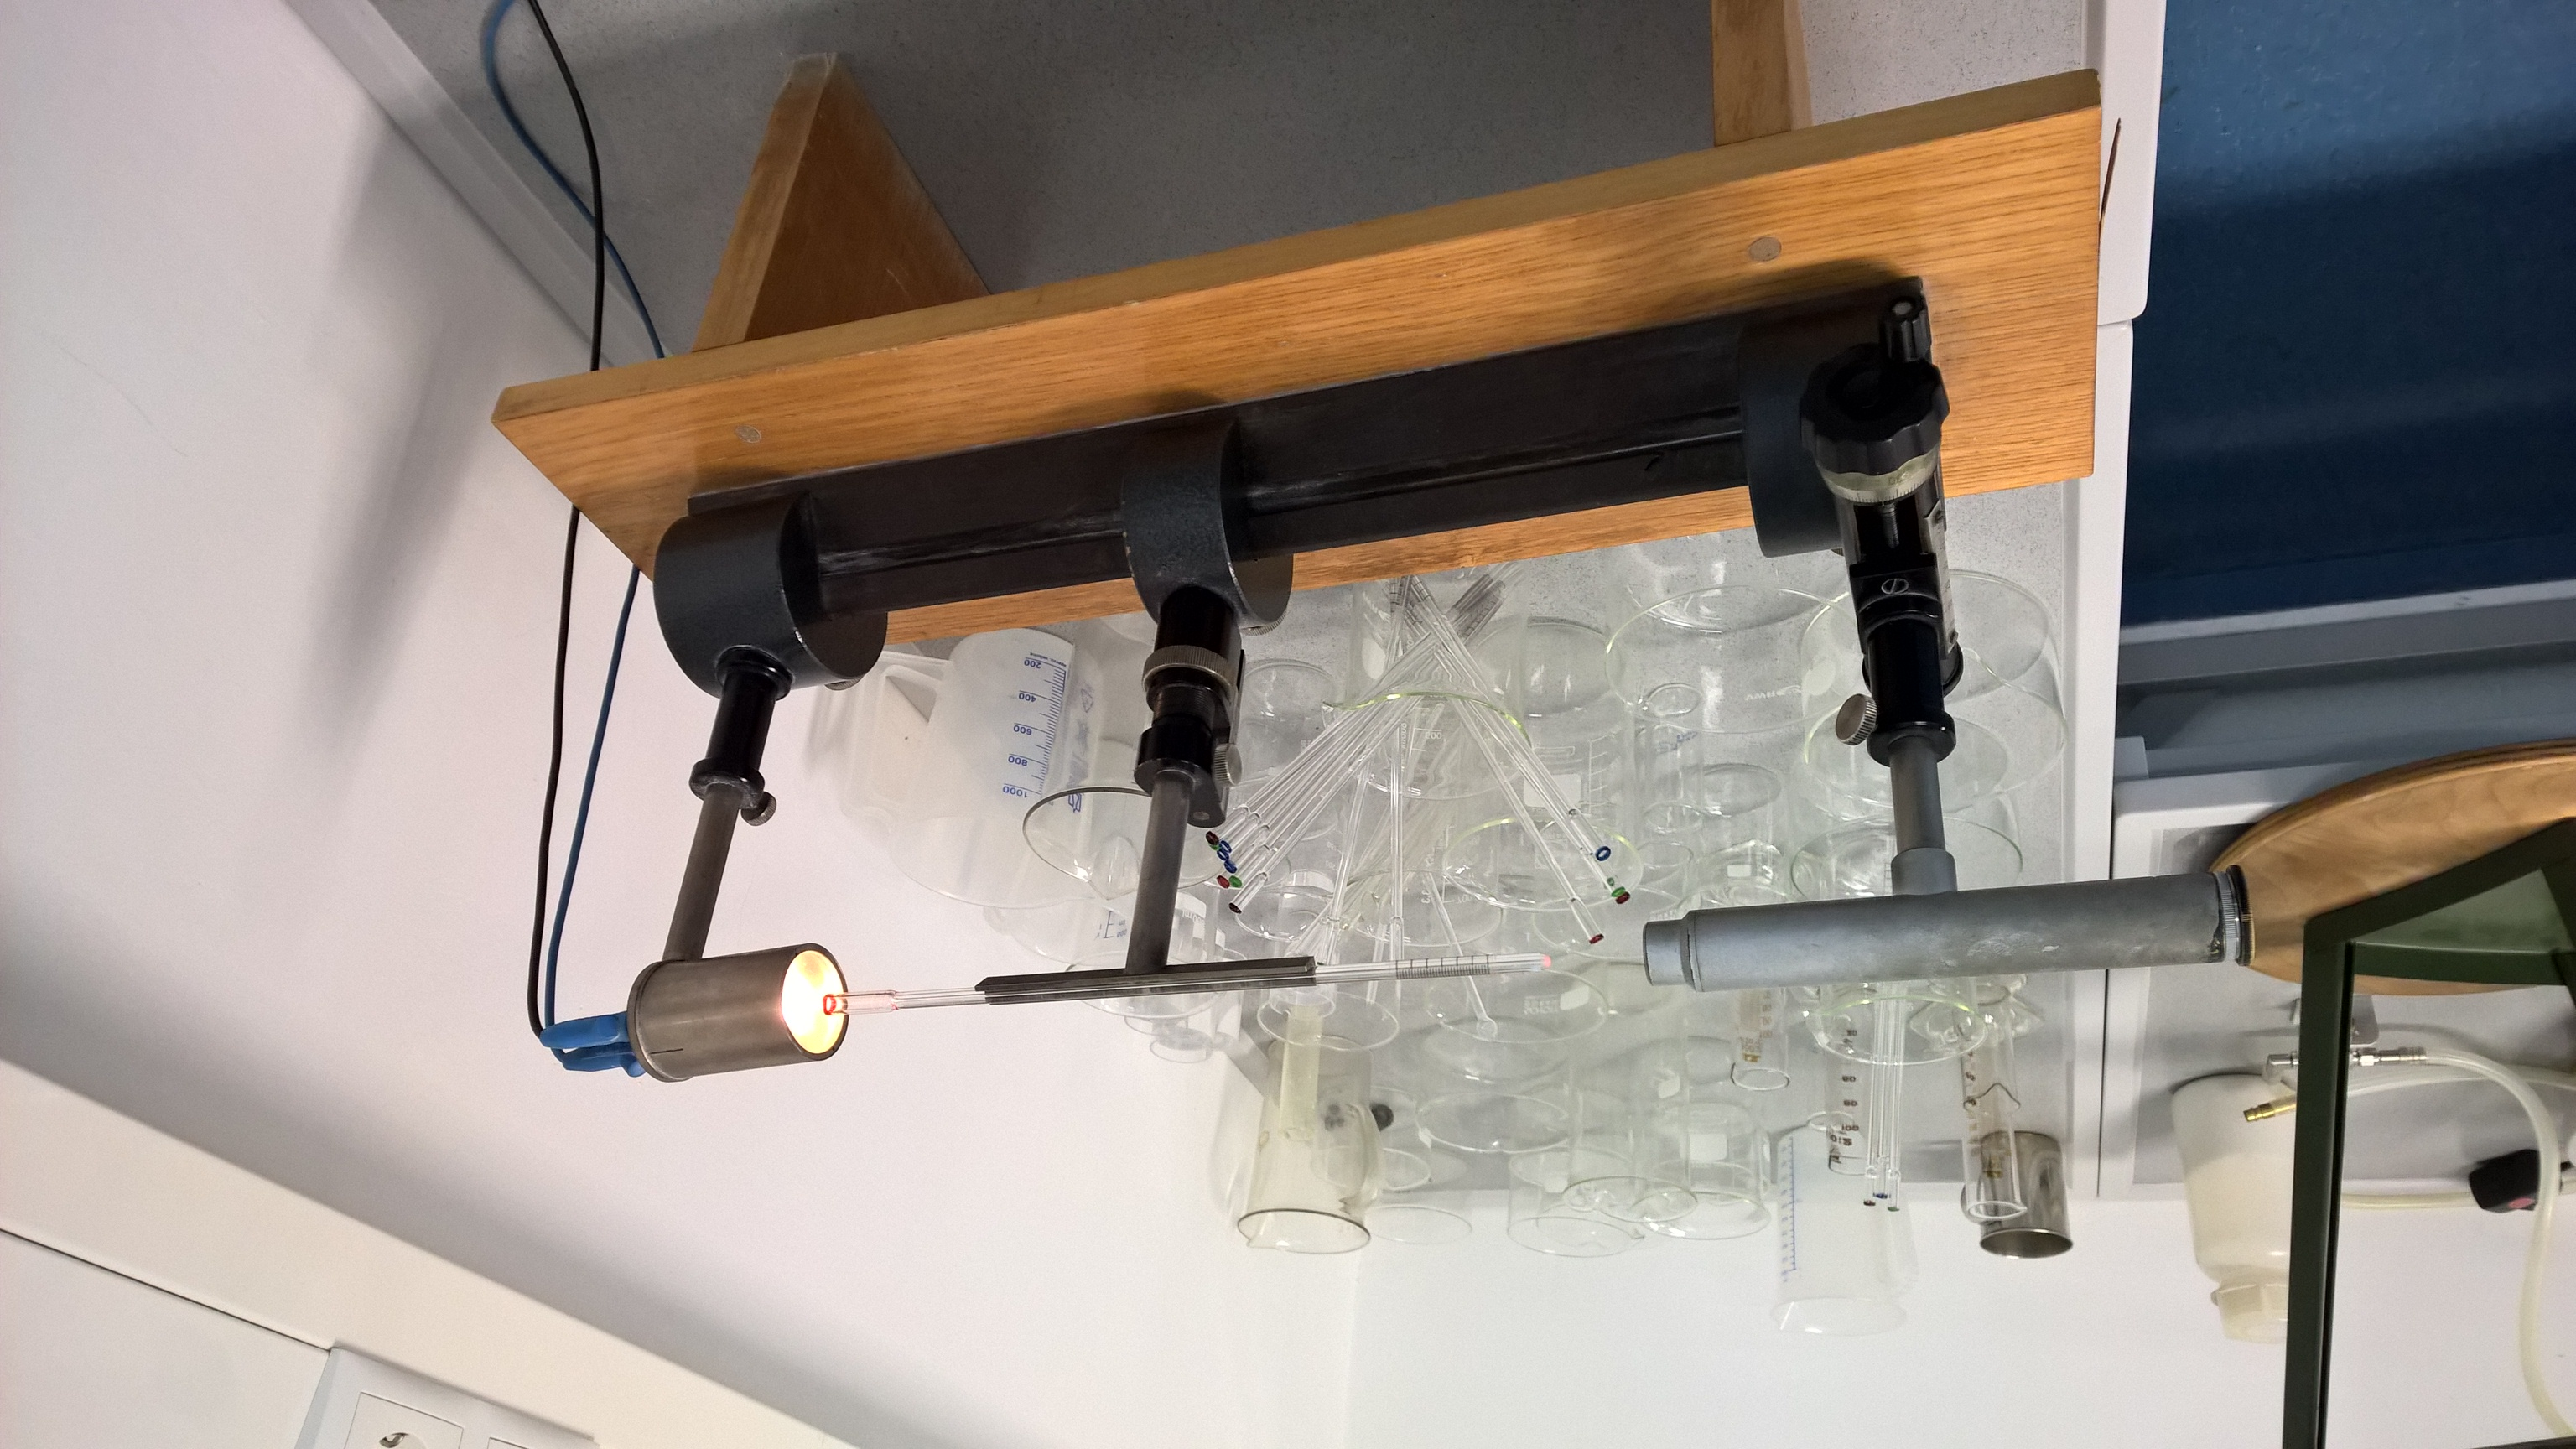
\includegraphics[width=0.7\textwidth]{Abbildungen/V7-1.jpg}
	\label{fig:V7-1}
\end{figure}

%
\begin{enumerate} \setcounter{enumi}{1}

 \begin{minipage}{0.5\textwidth}
	\item Wiegen Sie das leere Auffanggefäß und die Probekörper (jeweils einmal). 
  %
	\item Füllen Sie das Becherglas mit dem schrägen Auslass bis zu dessen Oberkante mit Wasser. Lassen Sie nun den Metallklotz in das Wasser und messen danach die Masse des Wassers im Auffanggefäß. \\
	Füllen Sie das Becherglas erneut bis zur Oberkante und lassen Sie den Holzklotz in das Wasser. Da er nicht komplett untergeht müssen Sie neben der Masse des ausgelaufenen Wassers auch die Eintauchtiefe und die Kantenlänge des Klotzes messen.
 \end{minipage}
 %
 \begin{minipage}{0.5\textwidth}
	\centering
	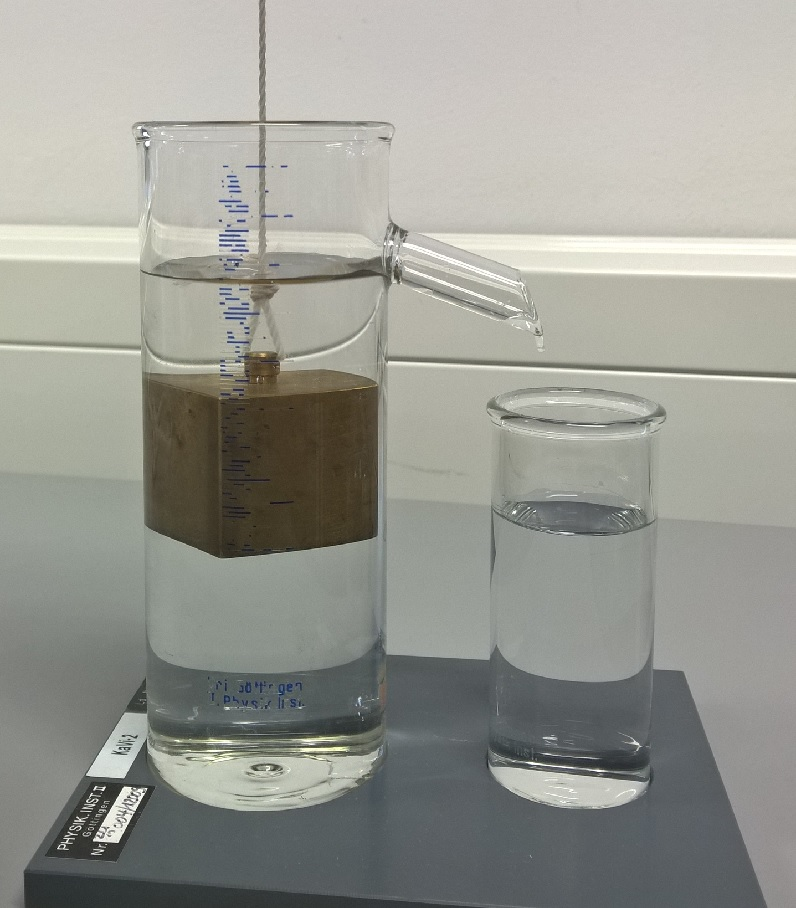
\includegraphics[width=0.7\textwidth]{Abbildungen/V7-2.jpg}
 \end{minipage}
 %
\end{enumerate}
%
\begin{hint}
	In den nachfolgenden Versuchsteilen (3 \& 4) geht es viel schneller wenn man jeweils die Versuche Steighöhen messen und Mohr'sche Waage hintereinander mit einer Flüssigkeit durchführt.
\end{hint}

Hier soll mit drei verschiedenen Flüssigkeiten gemessen werden: Wasser, Äthylenglykol, Methylalkohol. Die letzten beiden befinden sich im Eingangsbereich des Versuchsraums.
%
\begin{enumerate} \setcounter{enumi}{3}
 %
 \item Die Kapillare mit dem mittleren Radius wird tief in die Flüssigkeit getaucht. Damit ist die Innenseite der Kapillaren benetzt. Dann wird sie bis zur unteren schwarzen Markierung an der Kapillaren aus der Flüssigkeit gezogen. Hier ist die Steighöhe (innerhalb der Kapillaren) der Flüssigkeit abzulesen (1 Strich = 1 mm). Danach wird die Kapillare wieder komplett eingetaucht und erneut für eine Messung herausgezogen. Es müssen hier 5 Werte für die Steighöhe für alle 3 Flüssigkeiten bestimmt werden.
 
\begin{minipage}{0.5\textwidth}
 \item Bestimmen Sie die Dichten $\rho_{Fl}$ der drei Flüssigkeiten mithilfe der Mohr'schen Waage:
  \begin{itemize}
   \item Zuerst muss die Waage justiert werden. Dazu wird das Eichgewicht ganz langsam und vorsichtig so geschraubt, dass die Waage mit angehängtem Probekörper wieder im Gleichgewicht ist. 
   \item Danach wird der Probekörper ganz (inkl. Öse) in die zu untersuchende Flüssigkeit getaucht. Beachten Sie dabei, dass der Probekörper nicht an die Wand des Gefäßes stößt.
  \end{itemize}
\end{minipage}
%
\begin{minipage}{0.5\textwidth}
	\centering
	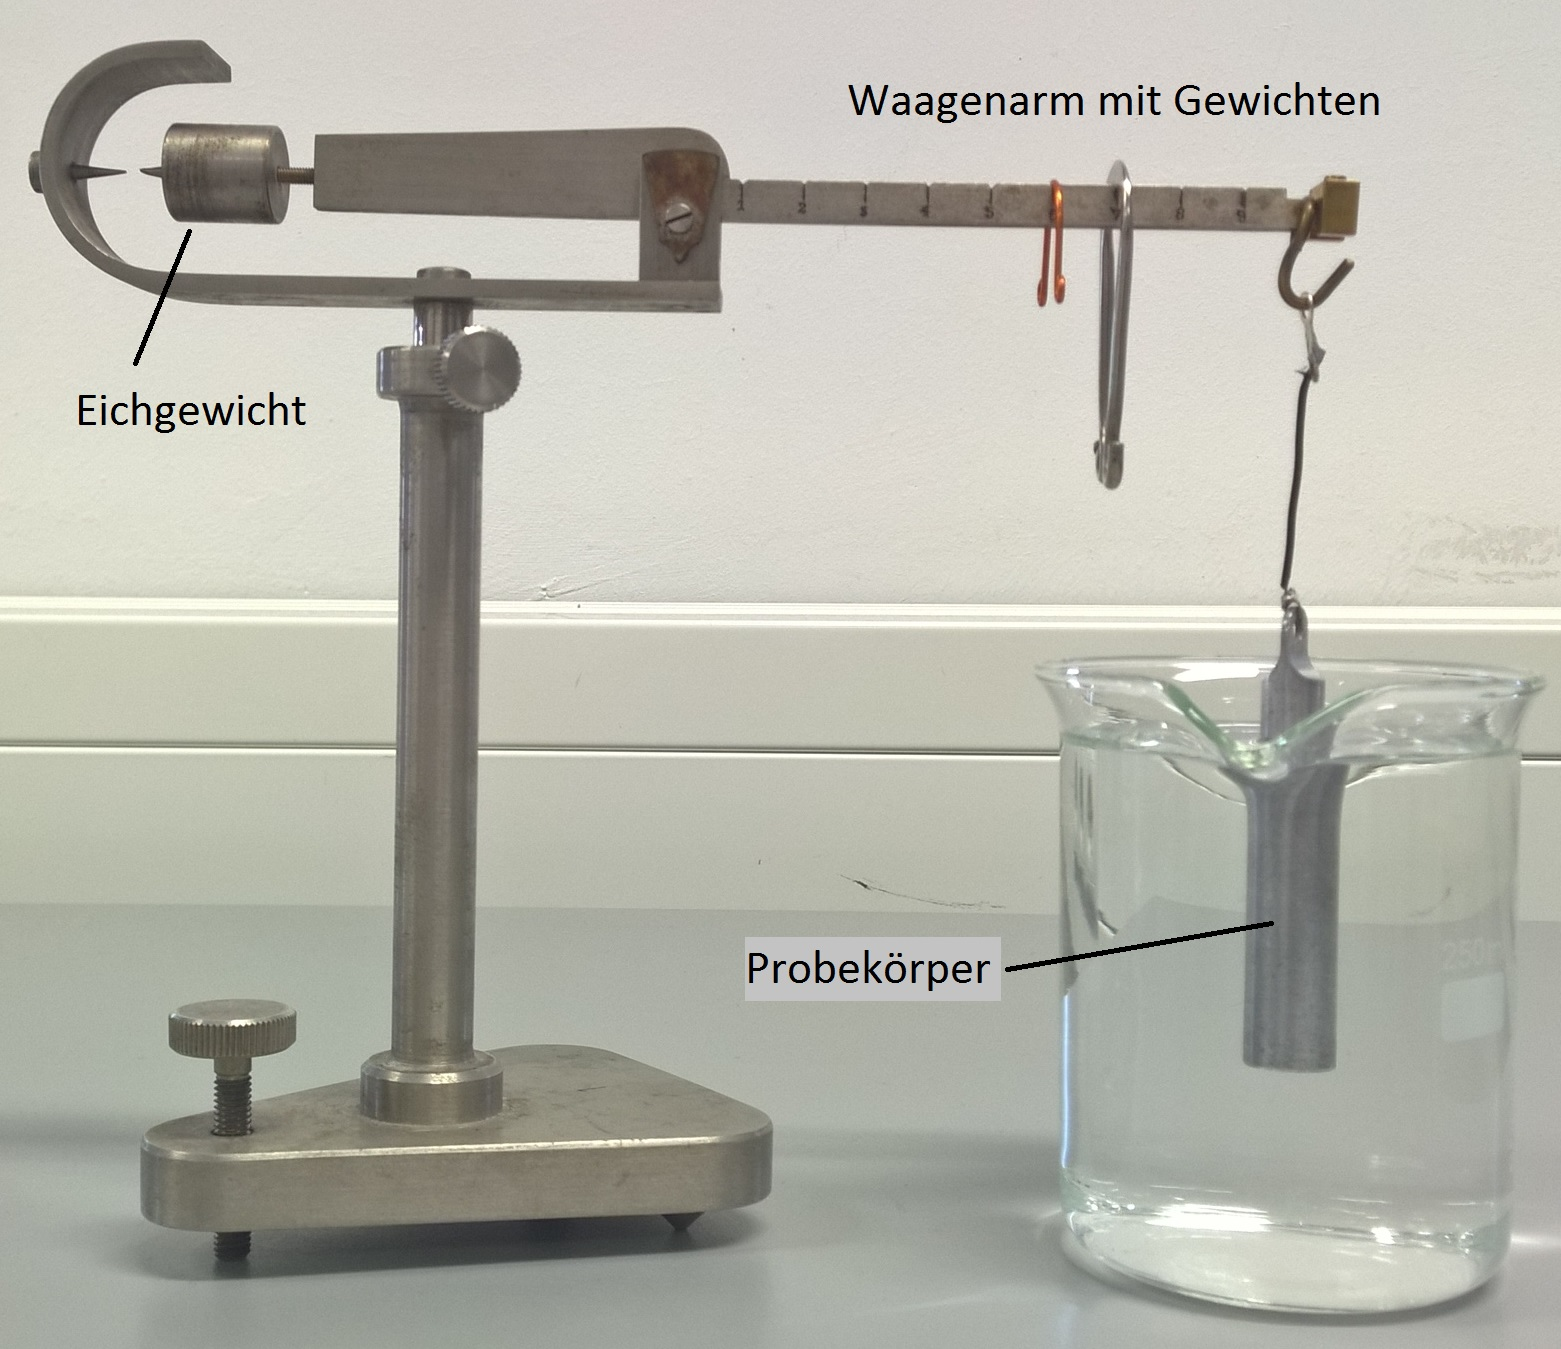
\includegraphics[width=0.8\textwidth]{Abbildungen/V7-3.jpg}
\end{minipage}

  Der Körper steigt aufgrund seines Auftriebs nach oben und bringt die Waage aus dem Gleichgewicht. Bringen Sie nun solange mit der Pinzette die gebogenen Gewichte an die verschiedenen Positionen des Waagenarms an, bis die Waage wieder im Gleichgewicht ist. Notieren Sie Lage (in cm) und Masse (in mg) der Gewichte.\\
  
  Beachten Sie, dass der Probekörper zwischen den Messungen mit verschiedenen Flüssigkeiten gründlich getrocknet werden muss. Warum?
 %
\end{enumerate}
%------------------------------------------------
\section{Auswertung} 
%------------------------------------------------
\etodo{Musterauswertung}
\begin{enumerate}
 %
 \item Bestimmen Sie die mittleren Radien $r_k$ der drei Typen von Kapillaren (blau, rot, grün) inklusive deren Fehler.
 %
 \item Berechnen Sie die Dichte $\rho_M$ des Metallkörpers inklusive Fehler.
 %
 \item Berechnen Sie die Dichte $\rho_H$ des Holzkörpers inklusive Fehler.
 %
 \item Berechnen Sie die Dichten $\rho_{Fl}$ von Äthylenglykol und Methylalkohol inklusive Fehler.
 %
 \item Bestimmen Sie die Oberflächenspannungen $\sigma$ von destilliertem Wasser, Methylalkohol und Äthylenglykol nach Gleichung \ref{eq:Oberflaechenspannung} und bestimmen Sie den Fehler von $\sigma$ aus den statistischen Messfehlern mittels Gauß'scher Fehlerfortpflanzung.
\end{enumerate}

\end{document}			% Linsengesetze
\chapter{Mikroskop}
\label{v:8}

Der Versuch erklärt die Funktionsweise des Lichtmikroskops, indem er die Beobachtung des reellen Zwischenbildes und des virtuellen Gesamtbildes ermöglicht. Auch das Grössenverhältnis von Bild und Gegenstand kann vermessen werden.

%------------------------------------------------
\section{Stichworte}
%------------------------------------------------

Reelles und virtuelles Bild; Vergrösserung; Okular, Objektiv; Numerische Apertur; Auflösungsvermögen.
%
%------------------------------------------------
\section{Literatur}
%------------------------------------------------

Gehrtsen, Kapitel 9.1.1/2, 9.2.4 bis 9.2.6 und 10.1.5
%
%------------------------------------------------
\section{Theoretischer Hintergrund}
%------------------------------------------------
\etodo{Mehr zum Hintergrund}

%Optische Geräte sind uns in vielfältiger Form aus dem täglichen Leben vertraut. Das Lichtmikroskop hatte darüber hinaus als Instrument der physikalischen, chemischen, medizinischen und biologischen Forschung eine herausragende Bedeutung. Es stellt in einem Zweistufenvorgang vergrößerte Bilder sehr kleiner Gegenstände her und ermöglicht somit die Sichtbarmachung ihrer Eigenschaften und Strukturen.\\
%
%\noindent
%Einer der bekanntesten Erfolge, die mit diesem Gerät erzielt wurden, ist die Entdeckung des Tuberkulose-Bakteriums durch Robert Koch im Jahre 1882. Für das Lichtmikroskop stellt die Beugung des Lichtes eine natürliche Grenze für das geometrische Auflösungsvermögen dar. Deshalb sind heute auch andere Mikroskope im Gebrauch, wie das Elektronenmikroskop oder das STM (Surface Tunneling Microscope).

Beim Mikroskop multiplizieren sich die Wirkungen zweier Linsen oder Linsensysteme. Das \textit{Objektiv} erzeugt ein möglichst großes reelles Zwischenbild des gut beleuchteten Gegenstandes. Im Prinzip könnte man schon dieses Bild beliebig groß machen, indem man den Gegenstand immer näher an die Brennebene der Objektivlinse rückt, was jedoch einige Nachteile hat:
\begin{itemize}
	\item Je größer das Zwischenbild wird, desto lichtärmer wird es. Damit wird es, selbst im dunklen Tubus des Mikroskops schwer zu erkennen.
	%
	\item Nach Gleichung \ref{eq:Abbildungsmassstab-Linse} wird bei gegebener Gegenstandsweite $g$ und -größe $G$ für eine große Bildgröße $B$ die Bildweite $b = t$, und damit die Länge des Tubus' $t$ sehr groß, was die Handhabung sehr unbequem macht.
	%
	\item Die Abbildungsfehler (sphärische und chromatische Aberration, Astigmatismus) werden größer.
	%
%	\item Durch das begrenzte Auflösungsvermögen
\end{itemize}
Der Gegenstand liegt also ganz knapp außerhalb der Objektivbrennweite $f_1$, so dass für den Abbildungsmaßstab gilt:
\begin{equation}
	\beta = \frac{B}{G} = \frac{b}{g} = \frac{t}{f_1}
\end{equation}
Offenbar muss also das Objektiv eine kleine Brennweite haben, damit das Zwischenbild groß wird. Hier liegt auch der Unterschied zum Teleskop, welches eine große Objektivbrennweite hat (Wieso?).

Dieses Zwischenbild betrachtet man mit dem \textit{Okular} als Lupe und erzielt somit eine nochmalige Vergrößerung $V_{ok}=s_0/f_2$, wobei $s_0~=~25$~cm der Abstand eines Gegenstandes vom Auge ist, bei dem man diesen mit entspanntem Auge noch scharf sehen kann. Das Zwischenbild muss dazu um die Brennweite $f_2$ hinter dem Okular sitzen.

Die Gesamtvergrößerung des Mikroskops ergibt sich aus dem Abbildungsmaßstab des Objektivs multipliziert mit der Lupenvergrößerung des Okulars zu
\begin{equation}
	V_{ges} = \frac{B}{G} = \frac{t}{f_1} \frac{s_0}{f_2}
\label{eq:Vergoesserung_Mikroskop}
\end{equation}

\subsection{Das Auflösungsvermögen optischer Geräte}

Jede Linse, begrenzt durch ihren Rand oder ihre Fassung, wirkt als beugende Öffnung (vgl. Versuch \ref{v:10}). Das bedeutet, dass sie auch von einem unendlich weit entfernten Punkt (z. Bsp. einem Stern) keinen absolut scharfen Bildpunkt erzeugt, sondern vielmehr ein \textit{Beugungsbild}. Die Breite des \textit{Hauptmaximums} der Intensität des Beugungsbildes hat einen Winkeldurchmesser von $1,22\frac{\lambda}{r}$, mit dem Radius $r$ der Linse. Zwei nahe beieinanderstehende Sterne lassen sich im Fernrohr nur als zwei getrennte Objekte erkennen, wenn ihre Beugungsscheibchen sich nicht überdecken.

Beim Mikroskop ist das Licht, das durch das Objektiv fällt, natürlich nicht parallel. Betrachtet man als Objekt einen hellen Punkt, so hat das Büschel der Lichtstrahlen, die durch das Objektiv treten einen Öffnungswinkel $\varphi$ mit der \textit{numerischen Apertur}
\begin{equation} \label{eq:num-Apertur}
	\sin\varphi = \frac{r}{f}\, ,
\end{equation} 
mit dem Radius $r$ der Objekivblende und dem Abstand $f$ zwischen Objekt und Objektiv, welcher ja fast gleich der Brennweite des Objektivs ist.\\
Der leuchtende Punkt erzeugt in der Zwischenbildebene ein Beugungsscheibchen mit einem Öffnungswinkel von $1,22\frac{\lambda}{r}$. Ein anderer leuchtender Punkt muss also mindestens um diesen Winkel, d.h. in der Objektebene um den Abstand $x_{min}~=~1,22f\lambda/r$ davon entfernt sein, damit die Scheibchen nicht verschmelzen. Mit der numerischen Apertur (s. Gleichung \ref{eq:num-Apertur}) kann man auch schreiben
%
\begin{equation}
	x_{min} \approx \frac{\lambda}{\sin\varphi}\, .
\end{equation}
%
Ein Mikroskop löst also umso besser auf, je kleiner die Wellenlänge $\lambda$ und je größer $\varphi$ ist.\\
Um die Vergrößerung kurzbrennweitiger Objektive auszunutzen, bringt man zwischen Objekt und Objektiv ein brechendes Medium (Immersionsöl), das die Wellenlänge auf $\lambda/n$ verringert. Dann ist
%
\begin{equation}
	x_{min} = \frac{\lambda}{n\,\sin\varphi} \, ,
\end{equation}
%
die numerische Apertur vergrößert sich auf $n\,\sin\varphi$.

Diese \textit{Beugungsbegrenzung} des Auflösungsvermögens wird als \textit{Auflösungsbegrenzung} oder \textit{Abbe-Limit} bezeichnet, nach Ernst Abbe, der diese Beziehung im 19. Jahrhundert beschrieb. Neuere Mikroskopieverfahren erreichen Auflösungen, die wesentlich unter diesem Abbe-Limit liegen, indem sie Details eines Präparates, die zu dicht nebeneinanderliegen, um optisch aufgelöst zu werden, nacheinander aufnehmen und das gesamte Bild im Nachhinein wieder zusammensetzen\footnote{Z. Bsp. Nobelpreis für Chemie, 2014, Stefan Hell zusammen mit Eric Betzig und William E. Moerner „for the development of super-resolved fluorescence microscopy“}. Dies bedeutet jedoch auf keinen Fall, dass das Abbe-Limit nicht mehr gilt, wie man manchmal hört. Vielmehr wird es nur in cleverer Art und Weise umgangen.

%------------------------------------------------
\section{Fragen zur Vorbereitung}
%------------------------------------------------

\begin{enumerate}
 %
 \item Was soll heute im Praktikum gemessen werden? Warum?
 %
 \item Wie ist die Vergrößerung einer Linse definiert?
 %
 \item Aus welchen Teilen ist ein optisches Mikroskop aufgebaut ? (kein Strahlengang)
 %
 \item Wieso macht man nicht schon das Zwischenbild sehr groß indem man den Gegenstand immer näher an die Brennebene des Objektivs heranrückt? Welche Probleme würden auftreten?
 % 1. Zwischenbild wird lichtschwächer
 % 2. Tubuslänge immer größer
 % 3. wachsende Abbildungsfehler
 % 4. beschränktes Auflösungsvermögen erlaubt nicht beliebig kleine Einzelheiten zu erkennen
 %
 \item Beschreiben Sie das Prinzip eines Elektronenmikroskops.
 %
 \item Beschreiben Sie das Prinzip eines Raster Tunnelmikroskops (RTM).
 %
 \item Konstruieren Sie den Strahlengang an der Lupe.
 %
 \item Konstruieren Sie den Strahlengang im Mikroskop. Was ist beim Fernrohr anders?
%
\end{enumerate}

%------------------------------------------------
\section{Durchführung} 
%------------------------------------------------

\begin{enumerate}
 %
 \item Messung der Gesamtvergrößerung $V_{ges}$ des Mikroskops:\\
  Betrachten Sie mit einem Auge einen Gegenstand $G$ (Objektmaßstab) bekannter Größe. Vergleichen Sie das Bild mit einem Maßstab $B$, der mit dem zweiten Auge neben dem Mikroskop zu sehen ist. Das Größenverhältnis von $B$ zu $G$ liefert die Vergrößerung:
  \[
  V_{ges} = \frac{B}{G}
  \]
  Wiederholen Sie die Messung drei Mal.
 %
 \item Messung der Objektivvergrößerung $V_{obj}$:\\
  Stellen Sie das Mikroskop so ein, dass der Objektmaßstab scharf abgebildet wird. Ändern Sie diese Einstellung danach nicht mehr!\\
  Benutzen Sie nun das geneigte Okular mit dem kurzen verschiebbaren Tubus mit Mattscheibe. Verschieben Sie die Mattscheibe, bis das reele Zwischenbild scharf ist. Hierzu verdunkeln Sie am besten den Raum. Messen Sie die Größe des Zwischenbildes, $B_Z$, mit der Schieblehre. Die Objektivvergrößerung ergibt sich nach:
  \[
  V_{obj} = \frac{B_Z}{G}
  \]
  Wiederholen Sie die Messung drei Mal.
 %
 \item Bestimmung der Objektivbrennweite $f_{obj}$:\\
  Benutzen Sie das Objektiv als Sammellinse und messen Sie die Größe des Zwischenbildes $B_Z$ für zwei Scharfeinstellungen auf der Mattscheibe:
  \begin{enumerate}
   \item mit dem kurzen Tubus: Setzen Sie den kurzen verschiebbaren Tubus mit Mattscheibe ein und messen Sie die Zwischenbildgröße $B_Z^{kurz}$ nachdem Sie das Bild scharf gestellt haben.
    \[
     V_{kurz} = \frac{B_Z^{kurz}}{G}
    \]
   %
   \item mit dem langen Tubus: Setzen Sie nun den langen Tubus mit Mattscheibe ein und messen Sie die Zwischenbildgröße $B_Z^{lang}$ nach erneuter Scharfstellung.
    \[
     V_{lang} = \frac{B_Z^{lang}}{G}
    \]
   %
   \item Messen Sie die Tubuslängen $t_1$ und $t_2$.
  \end{enumerate}
 %
 \item Bestimmung der Dicke eines Haares:\\
  Setzen Sie den kurzen verschiebbaren Tubus mit Mattscheibe ein und messen Sie die Zwischenbildgröße eines Haares mit der Schieblehre. 
\end{enumerate}

%------------------------------------------------
\section{Auswertung} 
%------------------------------------------------

\begin{enumerate}
%
\item Zeichnen Sie den Strahlengang im Mikroskop. Beschriften sie alle Brennpunkte, Gegenstands- und Bildgröße sowie die dazugehörige Gegenstands- und Bildweite.\\
Tip: Nutzen sie zur Konstruktion des Strahlengangs nur Parallel- bzw. Brennpunkt- und Mittelpunkstrahlen.
%
\item Berechnen Sie aus der Gesamtvergrößerung $V_{ges} = V_{obj}\cdot V_{ok}$ nun die Okularvergrößerung.\\
Berechnen sie die Fehler $\Delta V_{ges}$ und $\Delta V_{obj}$ über die Standardabweichung des Mittelwerts. Berechnen sie nun $\Delta V_{ok}$ mithilfe der Fehlerfortpflanzung. Leiten sie die dafür nötigen Ableitungen explizit her!
%
\item Berechnen Sie die Brennweite des Objektivs mit:
\begin{equation*}
f_{obj} = \left(t_2-t_1\right)\cdot\left(V_{lang}- V_{kurz}\right)
\end{equation*}
Berechnen Sie den Fehler auf die Brennweite.
%
\item Berechnen Sie die Dicke des Haares mithilfe der gemessenen Vergrößerung $V_{kurz}$.
%
\item Diskutieren sie entscheidende Fehlerquellen in diesem Versuch.
%
\end{enumerate}			% Mikroskop

\chapter{Brechungsindex von Glas}
\label{v:9}

In diesem Versuch untersuchen Sie die wellenlängenabhängige Beugung (Dispersion) von Licht in einem Glasprisma.

%------------------------------------------------
\section{Stichworte}
%------------------------------------------------

Reflexion; Brechungsgesetz nach Snellius; Huygenssches Prinzip; Dispersion; Brechungsindex; Minimalablenkwinkel.
%
%------------------------------------------------
\section{Literatur}
%------------------------------------------------

Gehrtsen, Kapitel 9.1.2 - 9.1.5
%
%------------------------------------------------
\section{Anwendungsbeispiele}
%------------------------------------------------
%
Optische Instrumente wie Linsen, Lichtleiter und Prismen werden seit jeher aus Glas oder Glas-ähnlichen Stoffen hergestellt. Ihre Funktion als optische Instrumente beruht dabei auf der Ausnutzung der unterschiedlichen Lichtgeschwindigkeit in Medien mit unterschiedlichem Brechungsindex $n$.\\
Luft wird dabei im Praktikum vereinfachend der Brechungsindex $n_{Luft} = 1$ zugeordnet. Das diese Annahme nicht immer stimmt sehen Sie am Flimmern der Luft über einer Flamme oder heißen Oberfläche, bzw. am Phänomen der Fata Morgana. 
%
%------------------------------------------------
\section{Theoretischer Hintergrund}
%------------------------------------------------

Fällt Licht auf die Grenzfläche zwischen zwei Medien (z.B. Luft und Glas), so kann es entweder reflektiert werden oder es dringt unter Änderung von Richtung, Geschwindigkeit und Wellenlänge ein. Ein Maß für diese Änderung ist der Brechungsindex $n$. Die Tatsache, dass $n$ für verschiedenfarbiges Licht verschieden ist, bezeichnet man als Dispersion; d.h. violettes Licht (kurze Wellenlänge) wird stärker abgelenkt als rotes Licht.

\subsection{Das Huygens-Fresnel'sche Prinzip und Brechung an Grenzflächen}

Die Wellenausbreitung im homogenen Medium und auch in komplizierteren Fällen lässt sich relativ intuitiv verstehen, wenn man sich nach \textit{Huygens} vorstellt, dass in jedem Punkt einer Wellenfront ein Streuzentrum sitzt, von welchem Kugelwellen (\textit{Elementarwellen}) ausgehen. Diese überlagern sich dann zu einer neuen Wellenfront.\\

\noindent
Diese Vorstellung kann man nachvollziehen, wenn man sich klar macht, wie das einfallende Licht die Atome der Materie beeinflusst. Licht besteht aus einer sich ausbreitenden elektromagnetischen Welle. Das bedeutet, dass mit dem Lichtstrahl ein sich schnell veränderndes elektrisches Feld einhergeht. Die Frequenz der Änderung des elektrischen Feldes ist dieselbe wie die, die wir dem Licht zuschreiben. Dieses elektrische Feld übt nun eine Kraft auf die Hüllenelektronen der Atome aus, indem es diese negativ geladenen Elektronen in Richtung des positiven elektrischen Feldes zu ziehen, es entsteht ein elektrisches Dipolmoment im Atom oder Molekül. Die schnellen Wechsel des elektrischen Feldes zwingen den Dipol dazu, mit derselben Frequenz zu schwingen. er ruft dadurch ein selbst ein oszillierendes elektrisches Feld hervor, welches dem Feld des einfallenden Lichtstrahls entgegengesetzt ist und dieses deshalb auslöscht. Gleichzeitig emittiert der Dipol aufgrund seiner Schwingung selbst wieder eine elektromagnetische Welle, welche dieselbe Frequenz hat, wie der ursprüngliche Lichtstrahl. Das sind die oben erwähnten Elementarwellen. Die von vielen Dipolen an der Oberfläche ausgesandten Elementarwellen überlagern sich nun konstruktiv und bilden eine ebene Wellenfront, wenn der Abstand zur Oberfläche groß gegenüber der Wellenlänge ist. Damit senden die vielen Dipole einen neuen Lichtstrahl aus, der dieselbe Frequenz hat wie der einfallende, sich jedoch in eine andere Richtung ausbreitet.\\

\noindent
Fällt eine ebene Welle schräg auf die ebene Grenze zwischen zwei Medien, in denen die Wellen unterschiedliche Ausbreitungsgeschwindigkeiten $c_1$ und $c_2$ haben, so haben die Elementarwellen in den beiden Medien nach einer bestimmten Zeit unterschiedliche Radien, welche sich wie $c_1/c_2$ verhalten (s. Abb. \ref{fig:brechung}). Damit nehmen die Überlagerungen der Elementarwellen, welche in dem jeweiligen Medium wieder ebene Wellenfronten bilden, verschiedene Winkel zum Lot auf die Grenzfläche ein. Bezeichnet $\alpha$ den Einfallswinkel und $\beta$ den Ausfallswinkel, dann erhalten wir das allgemeingültige Brechungsgesetz nach Snellius:
\begin{equation} \label{eq:Brechungsgesetz}
\frac{\sin\alpha}{\sin\beta} = \frac{c_1}{c_2}
\end{equation}

\begin{figure}[hb]
	\centering
		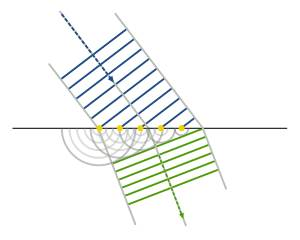
\includegraphics[width=.5\textwidth]{Versuch_9-10/Abbildungen/Brechung.jpg}
	\caption{Lichtbrechung mit Huygens'schem Prinzip. Im Medium oberhalb der Grenzfläche beträgt die Lichtgeschwindigkeit $c_1$, darunter $c_2$. Quelle: Wikimedia, Autor Arne Nordmann}
	\label{fig:brechung}
\end{figure}

\subsection{Brechungsindex und Snellius'sches Brechungsgesetz}

Der Brechungsindex $n$ eines Mediums kann "uber die Geschwindigkeit der Lichtwellen in diesem Medium definiert werden als:
\begin{equation}
n = \frac{c_0}{c_m}\, ,
\end{equation}
wobei $c_0$ die Lichtgeschwindigkeit im Vakuum bezeichnet und $c_m$ die Lichtgeschwindigkeit im Medium.\\

\noindent
Mit dieser Definition wird aus Gleichung \ref{eq:Brechungsgesetz} das \textit{Snellius'sche Brechungsgesetz}
\begin{equation} \label{eq:Snellius}
\frac{\sin\alpha_1}{\sin\alpha_2} = \frac{n_2}{n_1} = \frac{c_1}{c_2}
\end{equation}

\subsection{Totalreflexion}

Aus dem Brechungsgesetz (Gl. \ref{eq:Snellius}) kann man sehen, dass es einen Einfallswinkel $\alpha_1$ gibt, bei dem Reflexion unmöglich wird.\\
Da beim Übergang vom optisch dichteren Medium (mit größerem Brechungsindex) ins optisch dünnere Medium das Licht vom Lot auf die Grenzfläche weg gebrochen wird ist der Ausfallswinkel $\alpha_2$ immer größer als der Einfallswinkel. Wird der Ausfallswinkel entsprechend Gl. \ref{eq:Snellius} gleich 90$^{\circ}$, so läuft das Licht entlang der Grenzfläche. Wird der Einfallswinkel noch größer erscheint die Grenzfläche reflektierend und das Licht wird gemäß dem Reflexionsgesetz 'Einfallswinkel gleich Ausfallswinkel' wieder in das optisch dichtere Medium zurück reflektiert.\\
Damit ist klar, dass für den Einfallswinkel, unter dem Totalreflexion auftritt, gelten muss:
\begin{equation}
	\sin\alpha_1 \geq \frac{n_2}{n_1}
\end{equation}

\subsection{Dispersion}

In vielen Medien, wie z. Bsp. Wasser und Glas, hängt der Brechungsindex des Mediums von der Wellenlänge, bzw. der Frequenz, des Lichtes ab: $n = n(\lambda)$. Diese Tatsache nennt man \textit{Dispersion}. Aus historischen Gründen bezeichnet man den Fall, dass der Brechungsindex mit abnehmender Wellenlänge zunimmt $\left( \frac{dn}{d\lambda}<0\right)$ als \textit{normale Dispersion}, den umgekehrten Fall $\left( \frac{dn}{d\lambda}>0\right)$ als \textit{anomale Dispersion} (Beachte: nicht anormal, sondern anomal).\\
In diesen Fällen gilt immer noch das Brechungsgesetz nach Snellius, so lange man für jede betrachtete Wellenlänge den korrespondierenden Brechungsindex einsetzt.\\

\noindent
Das klassische Beispiel für Dispersion in der Natur ist der Regenbogen. Wir sehen einen Regenbogen vor uns, wenn die Sonne nicht zu hoch und hinter uns steht und es vor uns regnet. In diesem Fall tritt ein weißer Lichtstrahl von der Sonne in einen Wassertropfen ein, wobei es zur Dispersion kommt. Das Licht wird an der uns abgewandten Seite des Tropfens total reflektiert und tritt in unsere Richtung wieder aus dem Tropfen aus, wobei die Dispersion wieder auftritt. Da kurzwelliges Licht (blau) stärker gebrochen wird als langwelliges (rot), kann man aus genügend großer Entfernung die verschiedenen Farben des Sonnenlichtes unter verschiedenen Winkeln, also scheinbar an verschiedenen Orten am Himmel sehen: Ein Regenbogen.

\subsection{Ein paar Worte zum Prisma}

Wenn ein Lichtstrahl symmetrisch durch das Prisma hindurchgeht, d.h. parallel zur Basis (s. Abb. \ref{fig:prisma2}), erfährt er die kleinste Ablenkung (Minimal-Ablenkungswinkel). In diesem Fall lässt sich eine geometrische Beziehung zwischen dem Brechungsindex $n$ des Prismas, dem brechenden Winkel $\epsilon$ des Prismas und dem Minimalablenkungswinkel $\delta$ aufstellen:
\begin{equation} \label{eq:Brechungsindex}
n = \frac{\sin\left(\frac{\delta + \epsilon}{2}\right)}{\sin\left(\frac{\epsilon}{2}\right)}
\end{equation}
Diese nennt man die \textit{Fraunhofer Formel}.\\

\noindent
Aufgrund der Dispersion des Glases hängt der Brechungswinkel von der Wellenlänge ab. Dieser Effekt wird beschrieben durch die \textit{Winkeldispersion} des Prismas:
\begin{equation}
	\frac{d\delta}{d\lambda} = \frac{\partial\delta}{\partial n} \frac{dn}{d\lambda}.
\end{equation}
Der erste Faktor kann aus der Fraunhoferschen Formel berechnet werden, der zweite $\frac{dn}{d\lambda}$ ist die Dispersion.
%------------------------------------------------
\section{Fragen zur Vorbereitung}
%------------------------------------------------

\begin{enumerate}
 %
% \item Was soll heute im Praktikum gemessen werden? Warum?
 %
 \item Welchen physikalischen Vorgang beschreibt das Snellius'sche Brechungsgesetz?
 %
 \item Wie ist der Brechungsindex definiert?
 %
 \item Wie hängen Wellenlänge und Frequenz einer Lichtwelle zusammen?
 %
 \item Was ist Dispersion?
 %
 \item Wann kann man Totalrefelxion beobachten?
 %
 \item Wie lässt sich der Winkel f"ur die Totalreflexion aus dem Snellius'schen Brechungsgesetz ableiten?
 %
 \item Wird im Prisma rotes oder blaues Licht stärker abgelenkt?
 %
\end{enumerate}

%------------------------------------------------
\section{Durchführung} 
%------------------------------------------------

Im Versuch wird der Brechungsindex n eines Glasprismas bestimmt, das auf einer Apparatur steht, mit der man Winkel zwischen Lichtstrahlen sehr genau messen kann.

\noindent
Das Fernrohr kann geschwenkt und die Stellung auf einer Gradeinteilung abgelesen werden. Die Einteilung der Scheibe ist auf 0,50\degree genau. Der Nonius umfasst 30 Skalenteile, so dass man auf eine Bogenminute genau ablesen kann.\\
Der Spalt sollte aus Intensitätsgründen nicht zu eng eingestellt werden. Der Spalt sollte breiter sein als das Fadenkreuz im Fernrohr.


\begin{enumerate}
 %
 \item Verschieben Sie den Tubus des Spaltes so lange, bis Sie mit dem Fernrohr ein scharfes Bild des beleuchteten Spaltes sehen.
%Herstellung von parallelem Licht\\
  %Dieser Versuchsteil muss sorgf"altig nach Anleitung durchgeführt werden, sonst werden Sie sp"ater keine vernünftigen Ergebnisse erhalten !
  %\begin{itemize}
   %\item Nehmen Sie das Okular aus dem Fernrohr und stellen Sie das Fadenkreuz bei entspanntem Auge scharf. Schauen Sie dazu am besten gegen einen strukturlosen Hintergrund.
   %\item Setzen Sie das Okular wieder ein und stellen Sie das Fernrohr am offenen Fenster auf unendlich ein. Jetzt sehen Sie gleichzeitig das Fadenkreuz und weit entfernte Gegenst"ande scharf und parallaxenfrei (bei seitlicher Bewegung des Auges verschiebt sich das Fadenkreuz nicht gegen den Hintergrund). \\
   %Mit dieser Einstellung wird paralleles Licht im Auge fokussiert.
   %\item Stellen Sie nun das Fernrohr direkt in den Strahlengang und verschieben Sie den Spalt so lange, bis Sie ihn durch das Fernrohr scharf sehen. Damit haben Sie den Spalt so eingestellt, dass er paralleles Licht emittiert.
  %\end{itemize}
 %
 %\item Messen Sie den (doppelten) brechenden Winkel $2\,\gamma$ des Prismas mit reflektiertem Licht (s. Abb.~\ref{fig:prisma1}). Wiederholen Sie die Messung drei Mal.
 %%
 %\item Messen Sie den (doppelten) minimalen Ablenkwinkel $2\,\delta$ f"ur die rote H$_2$-Linie ($\lambda = 656,7$\,nm) und die blaue H$_2$-Linie ($\lambda = 486,1$\,nm). Wiederholen Sie die Messungen jeweils drei Mal. S. Abb. \ref{fig:prisma2}.\\
 %Den minimalen Ablenkwinkel erkennt man wie folgt: Beobachtung der roten H$_2$-Linie. Das Prisma wird in eine Richtung gedreht. Dabei erkennt man, dass diese Linie über eine bestimmte Stelle nicht hinauswandert. Diese Stelle ist diejenige, die dem Winkel der Minimalablenkung zugeordnet werden kann.
 %
% \item Beobachten Sie das Spektrum der Wasserstoff-Lampe.\\
%		Die Tatsache, dass das von angeregten Gasen emittierte Licht kein kontinuierliches Spektrum aufweist, sondern aus diskreten Spektrallinien zusammengesetzt ist, ist die Grundlage der Spektroskopie, welche unter anderem in  Chemie, Physik und Astronomie eine bedeutende Rolle spielt.
%\end{enumerate}
%
%\textbf{Alternativ:}
%
%\begin{enumerate}
	\item Beleuchten Sie den Spalt mit der Hg-Cd Lampe und lesen Sie auf dem Nonius den Winkel ab, unter dem Sie direkt das Bild des Spaltes sehen. \label{task:Spaltbild}
	%
	\item Stellen Sie das Prisma so in den Strahl, dass das Licht wie in Abb. \ref{fig:prisma2} gezeigt durch das Prisma fällt. Stellen Sie durch Drehen das Prisma auf den minimalen Ablenkwinkel für die gelbe Doppellinie der Hg-Cd Lampe ein. Verkleinern Sie die Spaltöffnung, bis Sie deutlich zwei Linien sehen. Notieren Sie die Winkel.
	%
	\item Arretieren Sie den Grobtrieb des Fernrohrs. 
	%
	\item Messen Sie den Ablenkwinkel der restlichen Linien im Spektrum der Hg-Cd Lampe mit dem Feintrieb des Fernrohrs. Schätzen Sie die Unsicherheit der Winkelmessung ab und notieren Sie diese. \label{task:HgSpektrum}
	%
	%\item Ersetzen Sie nun die Hg-Cd Lampe durch die Wasserstofflampe.
	%%
	%\item Messen Sie die Winkel der sichtbaren Spektrallinien der Wasserstofflampe.
\end{enumerate}

%------------------------------------------------
\section{Auswertung} 
%------------------------------------------------

\begin{enumerate}
 %%
 %\item Berechnen Sie den Mittelwert des brechenden Winkels $\overline{\gamma}$ inklusive seines Fehlers. Beachten Sie, dass Sie für die Berechnung des Fehlers den Winkel im Bogenmaß benutzen müssen.
 %%
 %\item Berechnen Sie die Mittelwerte des minimalen Ablenkwinkels $\overline{\delta}$ f"ur die rote und die blaue Wasserstofflinie inklusive der Fehler.
 %%
 %\item Nehmen Sie an, dass der Brechungsindex von Luft $n=1,0$ betr"agt. Berechnen Sie den Brechungsindex des Glases f"ur die rote und die blaue Wasserstofflinie, inklusive des jeweiligen Fehlers. Rechnen Sie daf"ur im Bogenma{\ss}.
 %%
 \item Korrigieren Sie die gemessenen Ablenkwinkel $\varphi$ aus Aufgabe \ref{task:HgSpektrum} um den Winkel aus Aufgabe \ref{task:Spaltbild}, um die wirklichen Ablenkwinkel $\delta$ zu bekommen.
 %
 \item Der Winkel der brechenden Kante des Prismas $\epsilon$ wird vom Hersteller mit 60\degree angegeben. Berechnen Sie aus den Ablenkwinkeln $\delta$ und dem Winkel der brechenden Kante des Prismas die jeweiligen Brechungsindizes mit Hilfe von Gleichung \ref{eq:Brechungsindex}. Berechnen Sie ebenfalls die Unsicherheit des Brechungsindex.
	%
 \item Tragen Sie die für die Hg-Cd Lampe gemessenen Brechungsindizes gegen die bekannten Wellenlängen der Spektrallinien auf.
 %
 \item Lesen Sie aus dem Diagramm die Dispersion $\frac{dn}{d\lambda}$ für blaues Licht und für gelbes Licht ab. Interpolieren Sie hierzu linear zwischen zwei geeigneten Wellenlängen. Wie groß ist die Unsicherheit?\\
	Der Hersteller gibt an:\\
	$\frac{dn}{d\lambda}|_{blau} = 2365\,\mathrm{cm^{-1}}$ sowie $\frac{dn}{d\lambda}|_{gelb} = 691\,\mathrm{cm^{-1}}$. Wie gut stimmen Ihre Werte mit den Herstellerangaben überein? Diskutieren Sie mögliche Abweichungen.
\end{enumerate}


\begin{table}[hb]
	\centering
		\begin{tabular}{lll}
			\hline
			Wellenlänge & Farbe & Intensität\\
			\hline
			643,85 nm & rot & stark\\
			579,07 nm & orangegelb & sehr stark\\
			576,96 nm & orangegelb & sehr stark\\
			546,07 nm & gelbgrün & stark\\
			508,58 nm & gelb & stark\\
			479,99 nm & blaugrün & stark\\
			467,82 nm & blau & mittel\\
			441,46 nm & blau & mittel\\
			407,78 nm & violett & stark\\
			\hline
		\end{tabular}
	\caption{Wellenlängen der Emissionslinien von Quecksilber und Cadmium}
	\label{tab:Wellenlaengen}
\end{table}

\begin{figure}[ht]
	\centering
		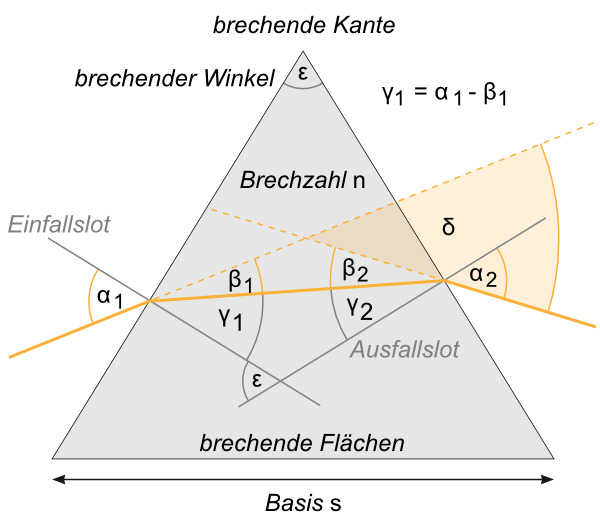
\includegraphics[width=.75\textwidth]{Versuch_9-10/Abbildungen/Hauptschnitt_lpgoe.jpg}
	\caption{Hauptschnitt durch ein Prisma. Quelle: Lehrportal Universität Göttingen}
	\label{fig:prisma2}
\end{figure}		% Brechungsindex von Glas
\documentclass[11pt, twoside, a4paper]{book}

\usepackage{graphicx}
\usepackage[utf8]{inputenc}
\usepackage{ngerman}
%\usepackage{lineno}
\usepackage{verbatim}
\usepackage[squaren]{SIunits}
\usepackage{amsmath}
\usepackage{amsfonts}
\usepackage{amssymb}
\usepackage{enumitem}
\usepackage{fancyhdr}
\usepackage{textcomp}
\usepackage{subcaption}
\usepackage[noadjust]{marginnote}
\usepackage{tikz}
\usepackage{nicefrac}
\usepackage{framed}
\usepackage{import}

\usetikzlibrary{calc,intersections}
\usetikzlibrary{arrows}
\usetikzlibrary{decorations.markings}
\usetikzlibrary{decorations.pathreplacing}
\usepackage[european resistors]{circuitikz}
\usepackage[ 
    top=2cm, 
    bottom=2cm, 
    outer=3cm, 
    inner=3cm,
    marginparwidth=2.5cm,
		headheight=14pt
  ]{geometry}

\usepackage{parskip}
\usepackage{pdfpages}

\setlength{\parindent}{0pt}

\newcommand{\experimentheader}[4]
{
  \iftutor{{\bf Schwierigkeitsgrad:} #1\\}
  \iftutor{{\bf Dauer:} #2\\}
  {\bf Ger\"ate:} #3\\
  {\bf Bauteile:} #4
}

\newcommand{\hintboxNone}{0}
\newcommand{\hintboxExclamation}{1}
\newenvironment{hintbox}[4][\hsize]
{
  \def\FrameCommand
  {%
    {\color{#3}\vrule width 3pt}%
    \hspace{0pt}%must no space.
    \fboxsep=\FrameSep\colorbox{#4}%
  }%
  \MakeFramed{\hsize#1\advance\hsize-\width\FrameRestore}%
  \mbox{\textbf{#2}:}%
}
{
  \endMakeFramed
}
\newcommand{\xhintbox}[3]
{
  \begin{hintbox}{Achtung}{red!50}{red!10}
    #3
  \end{hintbox}
}

\newenvironment{hint}
{
  \begin{hintbox}{Hinweis}{green!50}{green!10}
}
{
  \end{hintbox}
}

\newenvironment{definition}
{
  \begin{hintbox}{Definition\\}{white!50}{white!10}
}
{
  \end{hintbox}
}

\newenvironment{important}
{
  \begin{hintbox}{Hinweis}{gray!50}{gray!10}
}
{
  \end{hintbox}
}

\newenvironment{jason}
{
  \begin{hintbox}{Achtung}{red!50}{red!10}
}
{
  \end{hintbox}
}

\newcommand{\mandatoryenumi}
{
  \renewcommand{\labelenumi}{\arabic{enumi}.} 
}
\newcommand{\optionalenumi}
{
  \renewcommand{\labelenumi}{$\bigstar$\quad\arabic{enumi}.} 
}
\newcommand{\mandatoryenumii}
{
  \renewcommand{\labelenumii}{(\alph{enumii})} 
}
\newcommand{\optionalenumii}
{
  \renewcommand{\labelenumii}{$\bigstar$\quad(\alph{enumii})} 
}
\newcommand{\icname}[1]{\mbox{\tt #1}}


  %\newcommand{\iftutor}[1]{}
\newcommand{\ifnotutor}[1]{#1}

  \newcommand{\iftutor}[1]{#1}
\newcommand{\ifnotutor}[1]{}


\newenvironment{tutorhint}{\comment}{\endcomment}
\newenvironment{todo}{\comment}{\endcomment}
\newenvironment{solution}{\comment}{\endcomment}
\iftutor
{
  \renewenvironment{todo}
  {
    \hintbox{Todo}{red!50!yellow!90}{red!50!yellow!20}
  }
  {
    \endhintbox
  }
  \renewenvironment{tutorhint}
  {
    \hintbox{Tutorenhinweis der Stunde}{blue!50}{blue!10}
  }
  {
    \endhintbox
  }
  \renewenvironment{solution}
  {
    \hintbox{L\"osung}{black!80}{black!5}
  }
  {
    \endhintbox
  }
}
\newcommand{\etutorhint}[1]
{
  \iftutor{
    \tutorhint
      #1
    \endtutorhint
  }
}
\newcommand{\esolution}[1]
{
  \iftutor
  {
    \solution
    #1
    \endsolution
  }
}
\newcommand{\etodo}[1]
{
  \iftutor
  {
    \todo
    #1
    \endtodo
  }
}



\begin{document}

\renewcommand{\thechapter}{\arabic{chapter}}
\setcounter{chapter}{9}
\def\chaptername{Versuch}

\chapter{Mikroskop}
\label{v:8}

Der Versuch erklärt die Funktionsweise des Lichtmikroskops, indem er die Beobachtung des reellen Zwischenbildes und des virtuellen Gesamtbildes ermöglicht. Auch das Grössenverhältnis von Bild und Gegenstand kann vermessen werden.

%------------------------------------------------
\section{Stichworte}
%------------------------------------------------

Reelles und virtuelles Bild; Vergrösserung; Okular, Objektiv; Numerische Apertur; Auflösungsvermögen.
%
%------------------------------------------------
\section{Literatur}
%------------------------------------------------

Gehrtsen, Kapitel 9.1.1/2, 9.2.4 bis 9.2.6 und 10.1.5
%
%------------------------------------------------
\section{Theoretischer Hintergrund}
%------------------------------------------------

Beim Mikroskop multiplizieren sich die Wirkungen zweier Linsen oder Linsensysteme. Das \textit{Objektiv} erzeugt ein möglichst großes reelles Zwischenbild des gut beleuchteten Gegenstandes. Im Prinzip könnte man schon dieses Bild beliebig groß machen, indem man den Gegenstand immer näher an die Brennebene der Objektivlinse rückt, was jedoch einige Nachteile hat:
\begin{itemize}
	\item Je größer das Zwischenbild wird, desto lichtärmer wird es. Damit wird es, selbst im dunklen Tubus des Mikroskops schwer zu erkennen.
	%
	\item Nach Gleichung \ref{eq:Abbildungsmassstab-Linse} wird bei gegebener Gegenstandsweite $g$ und -größe $G$ für eine große Bildgröße $B$ die Bildweite $b = t$, und damit die Länge des Tubus' $t$ sehr groß, was die Handhabung sehr unbequem macht.
	%
	\item Die Abbildungsfehler (sphärische und chromatische Aberration, Astigmatismus) werden größer.
	%
%	\item Durch das begrenzte Auflösungsvermögen
\end{itemize}
Der Gegenstand liegt also ganz knapp außerhalb der Objektivbrennweite $f_1$, so dass für den Abbildungsmaßstab gilt:
\begin{equation}
	\beta = \frac{B}{G} = \frac{b}{g} = \frac{t}{f_1}
\end{equation}
Offenbar muss also das Objektiv eine kleine Brennweite haben, damit das Zwischenbild groß wird. Hier liegt auch der Unterschied zum Teleskop, welches eine große Objektivbrennweite hat (Wieso?).

Dieses Zwischenbild betrachtet man mit dem \textit{Okular} als Lupe und erzielt somit eine nochmalige Vergrößerung $V_{ok}=s_0/f_2$, wobei $s_0~=~25$~cm der Abstand eines Gegenstandes vom Auge ist, bei dem man diesen mit entspanntem Auge noch scharf sehen kann. Das Zwischenbild muss dazu um die Brennweite $f_2$ hinter dem Okular sitzen.

Die Gesamtvergrößerung des Mikroskops ergibt sich aus dem Abbildungsmaßstab des Objektivs multipliziert mit der Lupenvergrößerung des Okulars zu
\begin{equation}
	V_{ges} = \frac{B}{G} = \frac{t}{f_1} \frac{s_0}{f_2}
\label{eq:Vergoesserung_Mikroskop}
\end{equation}

\subsection{Das Auflösungsvermögen optischer Geräte}

Jede Linse, begrenzt durch ihren Rand oder ihre Fassung, wirkt als beugende Öffnung (vgl. Versuch \ref{v:10}). Das bedeutet, dass sie auch von einem unendlich weit entfernten Punkt (z. Bsp. einem Stern) keinen absolut scharfen Bildpunkt erzeugt, sondern vielmehr ein \textit{Beugungsbild}. Die Breite des \textit{Hauptmaximums} der Intensität des Beugungsbildes hat einen Winkeldurchmesser von $1,22\frac{\lambda}{r}$, mit dem Radius $r$ der Linse. Zwei nahe beieinanderstehende Sterne lassen sich im Fernrohr nur als zwei getrennte Objekte erkennen, wenn ihre Beugungsscheibchen sich nicht überdecken.

Beim Mikroskop ist das Licht, das durch das Objektiv fällt, natürlich nicht parallel. Betrachtet man als Objekt einen hellen Punkt, so hat das Büschel der Lichtstrahlen, die durch das Objektiv treten einen Öffnungswinkel $\varphi$ mit der \textit{numerischen Apertur}
\begin{equation} \label{eq:num-Apertur}
	\sin\varphi = \frac{r}{f}\, ,
\end{equation} 
mit dem Radius $r$ der Objekivblende und dem Abstand $f$ zwischen Objekt und Objektiv, welcher ja fast gleich der Brennweite des Objektivs ist.\\
Der leuchtende Punkt erzeugt in der Zwischenbildebene ein Beugungsscheibchen mit einem Öffnungswinkel von $1,22\frac{\lambda}{r}$. Ein anderer leuchtender Punkt muss also mindestens um diesen Winkel, d.h. in der Objektebene um den Abstand $x_{min}~=~1,22f\lambda/r$ davon entfernt sein, damit die Scheibchen nicht verschmelzen. Mit der numerischen Apertur (s. Gleichung \ref{eq:num-Apertur}) kann man auch schreiben
%
\begin{equation}
	x_{min} \approx \frac{\lambda}{\sin\varphi}\, .
\end{equation}
%
Ein Mikroskop löst also umso besser auf, je kleiner die Wellenlänge $\lambda$ und je größer $\varphi$ ist.\\
Um die Vergrößerung kurzbrennweitiger Objektive auszunutzen, bringt man zwischen Objekt und Objektiv ein brechendes Medium (Immersionsöl), das die Wellenlänge auf $\lambda/n$ verringert. Dann ist
%
\begin{equation}
	x_{min} = \frac{\lambda}{n\,\sin\varphi} \, ,
\end{equation}
%
die numerische Apertur vergrößert sich auf $n\,\sin\varphi$.

Diese \textit{Beugungsbegrenzung} des Auflösungsvermögens wird als \textit{Auflösungsbegrenzung} oder \textit{Abbe-Limit} bezeichnet, nach Ernst Abbe, der diese Beziehung im 19. Jahrhundert beschrieb. Neuere Mikroskopieverfahren erreichen Auflösungen, die wesentlich unter diesem Abbe-Limit liegen, indem sie Details eines Präparates, die zu dicht nebeneinanderliegen, um optisch aufgelöst zu werden, nacheinander aufnehmen und das gesamte Bild im Nachhinein wieder zusammensetzen\footnote{Z. Bsp. Nobelpreis für Chemie, 2014, Stefan Hell zusammen mit Eric Betzig und William E. Moerner „for the development of super-resolved fluorescence microscopy“}. Dies bedeutet jedoch auf keinen Fall, dass das Abbe-Limit nicht mehr gilt, wie man manchmal hört. Vielmehr wird es nur in cleverer Art und Weise umgangen.

\begin{tutorhint}
%------------------------------------------------
\section{Fragen zur Vorbereitung}
%------------------------------------------------

\begin{enumerate}
 %
 \item Was soll heute im Praktikum gemessen werden? Warum?
 %
 \item Wie ist die Vergrößerung einer Linse definiert?
 %
 \item Aus welchen Teilen ist ein optisches Mikroskop aufgebaut ? (kein Strahlengang)
 %
 \item Wieso macht man nicht schon das Zwischenbild sehr groß indem man den Gegenstand immer näher an die Brennebene des Objektivs heranrückt? Welche Probleme würden auftreten?
 % 1. Zwischenbild wird lichtschwächer
 % 2. Tubuslänge immer größer
 % 3. wachsende Abbildungsfehler
 % 4. beschränktes Auflösungsvermögen erlaubt nicht beliebig kleine Einzelheiten zu erkennen
 %
 \item Beschreiben Sie das Prinzip eines Elektronenmikroskops.
 %
 \item Beschreiben Sie das Prinzip eines Raster Tunnelmikroskops (RTM).
 %
 \item Konstruieren Sie den Strahlengang an der Lupe.
 %
 \item Konstruieren Sie den Strahlengang im Mikroskop. Was ist beim Fernrohr anders?
%
\end{enumerate}
\end{tutorhint}

%------------------------------------------------
\section{Durchführung} 
%------------------------------------------------




\begin{enumerate}
 %
\begin{minipage}{0.5\textwidth}
 \item Messung der Gesamtvergrößerung $V_{ges}$ des Mikroskops:\\
  Betrachten Sie mit einem Auge einen Gegenstand $G$ (Objektmaßstab) bekannter Größe. Vergleichen Sie das Bild mit einem Maßstab $B$, der mit dem zweiten Auge neben dem Mikroskop zu sehen ist. Das Größenverhältnis von $B$ zu $G$ liefert die Vergrößerung:
  \[
  V_{ges} = \frac{B}{G}
  \]
  Wiederholen Sie die Messung drei Mal.
	%
	\item Messung der Objektivvergrößerung $V_{obj}$:\\
  Stellen Sie das Mikroskop so ein, dass der Objektmaßstab scharf abgebildet wird. Ändern Sie diese Einstellung danach nicht mehr!\\
\end{minipage}
%
\begin{minipage}{0.5\textwidth}
	\centering
		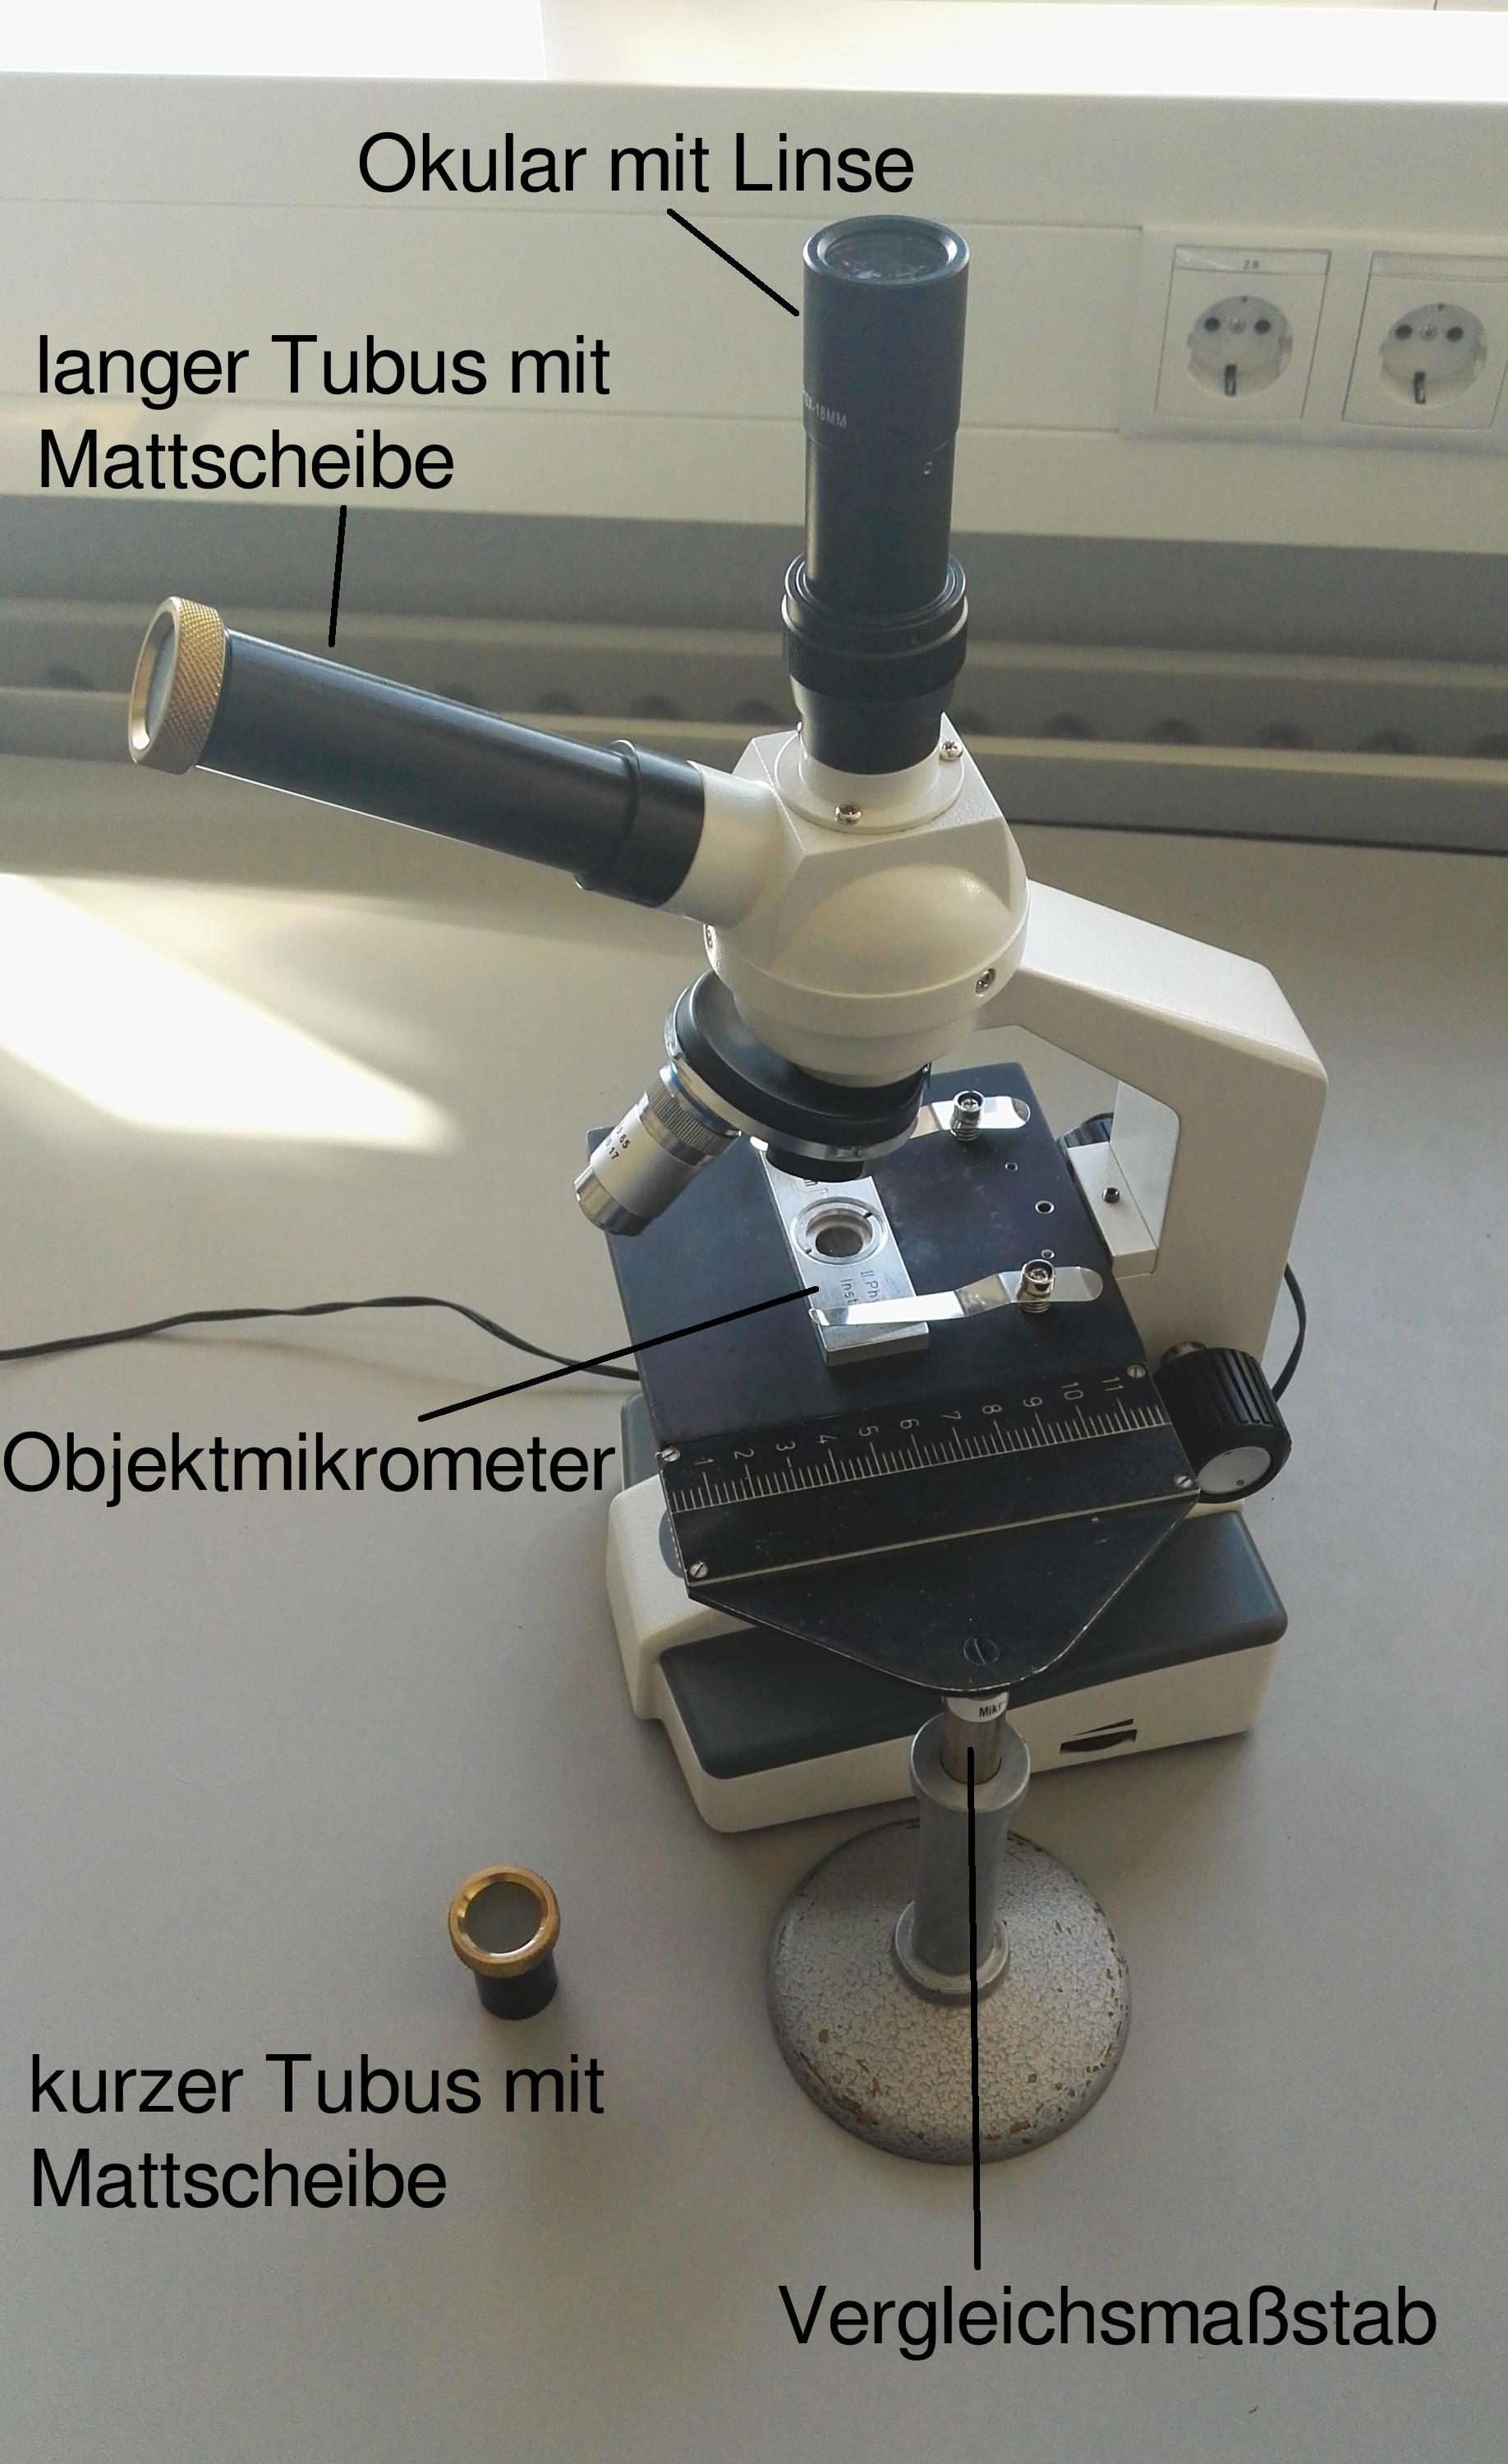
\includegraphics[width=0.7\textwidth]{Abbildungen/mikroskopbildA.jpg}
	\label{fig:mikroskopbildA}
\end{minipage}
 
	Benutzen Sie nun das geneigte Okular mit dem kurzen verschiebbaren Tubus mit Mattscheibe. Verschieben Sie die Mattscheibe, bis das reele Zwischenbild scharf ist. Hierzu verdunkeln Sie am besten den Raum. Messen Sie die Größe des Zwischenbildes, $B_Z$, mit der Schieblehre. Die Objektivvergrößerung ergibt sich nach:
  \[
  V_{obj} = \frac{B_Z}{G}
  \]
  Wiederholen Sie die Messung drei Mal.
 %
 \item Bestimmung der Objektivbrennweite $f_{obj}$:\\
  Benutzen Sie das Objektiv als Sammellinse und messen Sie die Größe des Zwischenbildes $B_Z$ für zwei Scharfeinstellungen auf der Mattscheibe:
  \begin{enumerate}
   \item mit dem kurzen Tubus: Setzen Sie den kurzen verschiebbaren Tubus mit Mattscheibe ein und messen Sie die Zwischenbildgröße $B_Z^{kurz}$ nachdem Sie das Bild scharf gestellt haben.
    \[
     V_{kurz} = \frac{B_Z^{kurz}}{G}
    \]
   %
   \item mit dem langen Tubus: Setzen Sie nun den langen Tubus mit Mattscheibe ein und messen Sie die Zwischenbildgröße $B_Z^{lang}$ nach erneuter Scharfstellung.
    \[
     V_{lang} = \frac{B_Z^{lang}}{G}
    \]
   %
   \item Messen Sie die Tubuslängen $t_1$ und $t_2$.
  \end{enumerate}
 %
 \item Bestimmung der Dicke eines Haares:\\
  Setzen Sie den kurzen verschiebbaren Tubus mit Mattscheibe ein und messen Sie die Zwischenbildgröße eines Haares mit der Schieblehre. 
\end{enumerate}

%------------------------------------------------
\section{Auswertung} 
%------------------------------------------------
\etodo{Musterauswertung}
\begin{enumerate}
%
\item Zeichnen Sie den Strahlengang im Mikroskop. Beschriften sie alle Brennpunkte, Gegenstands- und Bildgröße sowie die dazugehörige Gegenstands- und Bildweite.\\
Tip: Nutzen sie zur Konstruktion des Strahlengangs nur Parallel- bzw. Brennpunkt- und Mittelpunkstrahlen.
%
\item Berechnen Sie aus der Gesamtvergrößerung $V_{ges} = V_{obj}\cdot V_{ok}$ nun die Okularvergrößerung.\\
Berechnen sie die Fehler $\Delta V_{ges}$ und $\Delta V_{obj}$ über die Standardabweichung des Mittelwerts. Berechnen sie nun $\Delta V_{ok}$ mithilfe der Fehlerfortpflanzung. Leiten sie die dafür nötigen Ableitungen explizit her!
%
\item Berechnen Sie die Brennweite des Objektivs mit:
\begin{equation*}
f_{obj} = \left(t_2-t_1\right)\cdot\left(V_{lang}- V_{kurz}\right)
\end{equation*}
Berechnen Sie den Fehler auf die Brennweite.
%
\item Berechnen Sie die Dicke des Haares mithilfe der gemessenen Vergrößerung $V_{kurz}$.
%
\item Diskutieren sie entscheidende Fehlerquellen in diesem Versuch.
%
\end{enumerate}

\end{document}		% Beugung am Gitter

\documentclass[11pt, twoside, a4paper]{book}

\usepackage{graphicx}
\usepackage[utf8]{inputenc}
\usepackage{ngerman}
%\usepackage{lineno}
\usepackage{verbatim}
\usepackage[squaren]{SIunits}
\usepackage{amsmath}
\usepackage{amsfonts}
\usepackage{amssymb}
\usepackage{enumitem}
\usepackage{fancyhdr}
\usepackage{textcomp}
\usepackage{subcaption}
\usepackage[noadjust]{marginnote}
\usepackage{tikz}
\usepackage{nicefrac}
\usepackage{framed}
\usepackage{import}

\usetikzlibrary{calc,intersections}
\usetikzlibrary{arrows}
\usetikzlibrary{decorations.markings}
\usetikzlibrary{decorations.pathreplacing}
\usepackage[european resistors]{circuitikz}
\usepackage[ 
    top=2cm, 
    bottom=2cm, 
    outer=3cm, 
    inner=3cm,
    marginparwidth=2.5cm,
		headheight=14pt
  ]{geometry}

\usepackage{parskip}
\usepackage{pdfpages}

\setlength{\parindent}{0pt}

\newcommand{\experimentheader}[4]
{
  \iftutor{{\bf Schwierigkeitsgrad:} #1\\}
  \iftutor{{\bf Dauer:} #2\\}
  {\bf Ger\"ate:} #3\\
  {\bf Bauteile:} #4
}

\newcommand{\hintboxNone}{0}
\newcommand{\hintboxExclamation}{1}
\newenvironment{hintbox}[4][\hsize]
{
  \def\FrameCommand
  {%
    {\color{#3}\vrule width 3pt}%
    \hspace{0pt}%must no space.
    \fboxsep=\FrameSep\colorbox{#4}%
  }%
  \MakeFramed{\hsize#1\advance\hsize-\width\FrameRestore}%
  \mbox{\textbf{#2}:}%
}
{
  \endMakeFramed
}
\newcommand{\xhintbox}[3]
{
  \begin{hintbox}{Achtung}{red!50}{red!10}
    #3
  \end{hintbox}
}

\newenvironment{hint}
{
  \begin{hintbox}{Hinweis}{green!50}{green!10}
}
{
  \end{hintbox}
}

\newenvironment{definition}
{
  \begin{hintbox}{Definition\\}{white!50}{white!10}
}
{
  \end{hintbox}
}

\newenvironment{important}
{
  \begin{hintbox}{Hinweis}{gray!50}{gray!10}
}
{
  \end{hintbox}
}

\newenvironment{jason}
{
  \begin{hintbox}{Achtung}{red!50}{red!10}
}
{
  \end{hintbox}
}

\newcommand{\mandatoryenumi}
{
  \renewcommand{\labelenumi}{\arabic{enumi}.} 
}
\newcommand{\optionalenumi}
{
  \renewcommand{\labelenumi}{$\bigstar$\quad\arabic{enumi}.} 
}
\newcommand{\mandatoryenumii}
{
  \renewcommand{\labelenumii}{(\alph{enumii})} 
}
\newcommand{\optionalenumii}
{
  \renewcommand{\labelenumii}{$\bigstar$\quad(\alph{enumii})} 
}
\newcommand{\icname}[1]{\mbox{\tt #1}}


  %\newcommand{\iftutor}[1]{}
\newcommand{\ifnotutor}[1]{#1}

  \newcommand{\iftutor}[1]{#1}
\newcommand{\ifnotutor}[1]{}


\newenvironment{tutorhint}{\comment}{\endcomment}
\newenvironment{todo}{\comment}{\endcomment}
\newenvironment{solution}{\comment}{\endcomment}
\iftutor
{
  \renewenvironment{todo}
  {
    \hintbox{Todo}{red!50!yellow!90}{red!50!yellow!20}
  }
  {
    \endhintbox
  }
  \renewenvironment{tutorhint}
  {
    \hintbox{Tutorenhinweis der Stunde}{blue!50}{blue!10}
  }
  {
    \endhintbox
  }
  \renewenvironment{solution}
  {
    \hintbox{L\"osung}{black!80}{black!5}
  }
  {
    \endhintbox
  }
}
\newcommand{\etutorhint}[1]
{
  \iftutor{
    \tutorhint
      #1
    \endtutorhint
  }
}
\newcommand{\esolution}[1]
{
  \iftutor
  {
    \solution
    #1
    \endsolution
  }
}
\newcommand{\etodo}[1]
{
  \iftutor
  {
    \todo
    #1
    \endtodo
  }
}



\begin{document}

\renewcommand{\thechapter}{\arabic{chapter}}
\setcounter{chapter}{10}
\def\chaptername{Versuch}

\chapter{Thermoelement}
\label{v:11}

Ein Thermoelement wandelt Wärme in elektrische Energie um. In diesem Versuch soll das Thermoelement zur Messung einer Temperatur benutzt werden.

%------------------------------------------------
\section{Stichworte}
%------------------------------------------------

Metallbindung; Austrittsarbeit; Fermienergie; Kontaktspannung; Thermospannung; Thermoelement; W"armebad.
%
%------------------------------------------------
\section{Literatur}
%------------------------------------------------

Gehrtsen, Kapitel 6.6.1, 8.1.1, 14.1.5, 14.3.1/2\\
R. Pelster, R. Pieper, I. Hüttl, \textit{Thermospannungen - Viel genutzt und fast immer falsch erklärt!}, PhyDid 1/4 (2005)

%------------------------------------------------
\section{Anwendungsbeispiele}
%------------------------------------------------

Thermoelemente werden zur Temperaturmessung in vielen verschiedenen Umgebungen benutzt, z. Bsp. in Flüssigkeiten verschiedenster Ph-Werte, in industriellen Anwendungen mit extremen Temperaturen und Atmosphären Zusammensetzungen. Sie werden aber auch zur hochgenauen Temperaturmessung im Labor verwendet.

%------------------------------------------------
\section{Theoretischer Hintergrund}
%------------------------------------------------

\textit{Thomas Johann Seebeck} l"otete 1821 zwei Dr"ahte aus verschiedenen Metallen zu einem Ring zusammen und fand, dass eine Temperaturdifferenz zwischen den beiden L"otstellen einen Strom antreibt.\\
In vielen Lehrbüchern, auch für Experimentalphysiker, sowie in älteren Versionen dieses Skripts, wird dieses Phänomen fälschlicherweise durch die unterschiedliche Auslösearbeit der Elektronen in den beiden Metallen erklärt. In Wirklichkeit liefert diese jedoch nur einen kleinen Beitrag zum gesammten Effekt. Hier legen wir eine vereinfachte, jedoch komplette Behandlung, dar, wie sie von Pelster et al. vorgestellt wurde.

\subsection{Thermodiffusion}

Betrachten wir zunächst einen Metallstab bei konstanter Temperatur. Die freien Ladungsträger, in diesem Fall Elektronen, sind homogen im Stab verteilt und führen eine ungeordnete Wärmebewegung (s. Browne'sche Bewegung, Maxwell Verteilung). Der Betrag der mittleren Geschwindigkeit hängt dabei von der Temperatur ab: Je wärmer der Körper, desto schneller bewegen sich die Elektronen.\\
Haben die Stabenden nun unterschiedliche Temperaturen, so ist die Geschwindigkeit der Elektronen am heißen Ende höher als am kalten Ende. Dies führt zu einer gerichteten Netto-Bewegung der Elektronen vom warmen zum kalten Ende des Stabes (vgl. Diffusion). Passenderweise nennt man diese Bewegung Thermodiffusion. Sie führt dazu, dass sich das kalte Ende des Stabes gegenüber dem warmen negativ auflädt. Die Aufladung wächst solange an, bis das sich aufbauende elektrische Feld stark genug ist, die Diffusion zu kompensieren: Der Diffusionsstrom kommt zum Erliegen.\\
Die Spannung zwischen den beiden Stabenden, die sogenannte Thermodiffusionsspannung, ist in erster Näherung proportional zur Temperaturdifferenz zwischen den Stabenden:
\begin{equation}
	U_{TD} = -Q\cdot \Delta T
\end{equation}
Der Proportionalitätsfaktor $Q$, der Seebeck-Koeffizient, ist materialspezifisch, d.h. es ergeben sich unterschiedlich große Spannungen je nachdem, welches Metall (oder Halbleiter) man betrachtet.

\subsection{Thermoelement}

Fügt man zwei Teilstücke aus unterschiedlichen Materialien zu einem Ring zusammen, so ergibt sich eine Schleife mit einem thermoelektrischen Kreisstrom. Beim Thermoelement ist ein Voltmeter in die Schleife geschaltet, so dass praktisch kein Strom fließt. Das Voltmeter zeigt dann die Thermospannung, i.e. die Differenz der beiden Thermodiffusionsspannungen:
\begin{equation}
	U_{Thermo} = U^A_{TD} - U^B_{TD}.
\end{equation}
Entfernt man das Voltmeter und schliesst den Kreis, so treibt diese Thermospannung einen Kreisstrom an. Dabei bestimmt das Material mit der größeren Thermodiffusionsspannung die Stromrichtung (ähnlich wie in einem Stromkreis mit zwei ungleichen gegeneinandergeschalteten Batterien).

%Wenn zwei verschiedene Metalle 1 und 2 einander ber"uhren, gehen einige Elektronen von einem zum anderen "uber. In welche Richtung mehr Elektronen "ubergehen h"angt von den Energien der h"ochsten besetzten Energiezust"ande (Fermie-Energie), d.h. der Austrittsarbeit der Elektronen ab. Das Metall mit der geringeren Austrittsarbeit (1) gibt Elektronen ab und wird somit positiv geladen. Der "Ubertritt h"ort erst auf, wenn sich eine \textit{Kontaktspannung} aufgebaut hat, die entgegengesetzt gleich der Differenz der Austrittsarbeiten ist. Dann treten in beide Richtungen gleich viele Elektronen "uber: von 1 nach 2 durch Diffusion, von 2 nach 1 infolge des elektrischen Feldes in der Grenzschicht.\\
%In einer vereinfachenden Betrachtung beschreibt man diese beiden Elektronengase durch die Boltzmann-Statistik (in Wirklichkeit gilt f"ur so dichte Gase die Fermi-Statistik). Diese ergibt f"ur die Kontaktspannung eine Abh"angigkeit vom Verh"altnis der Teilchenzahldichten:
%\begin{equation} \label{eq:Kontaktspannung}
% \frac{n_1}{n_2} = e^{-e\,\Delta U/(kT)} \; \Rightarrow \; \Delta U = \frac{kT}{e}\ln\frac{n_2}{n_1}
%\end{equation}
%Wie man sieht, h"angt die Kontaktspannung auch von der Temperatur der Kontaktstelle ab.\\

%\noindent
%Biegt man die beide Dr"ahte zu einem Ring, so bildet sich an beiden Kontaktstellen eine Kontaktspannung aus. Da beide Spannungen aber entgegengesetzt  geschaltet sind, flie{\ss}t im Ring kein Strom.\\
%Erw"armt man aber eine der Kontaktstellen, dann werden die beiden Kontaktspannungen laut Gleichung \ref{eq:Kontaktspannung} trotz gleichen Verh"altnisses $n_2/n_1$ unterschiedlich, und es flie{\ss}t ein \textit{Thermostrom}. Die daf"ur ben"otigte Energie wird der W"armequelle entnommen.\\
%L"otet man also zwei Dr"ahte aus verschiedenen Metallen an beiden Enden zusammen und schaltet in den einen Draht ein Voltmeter, so zeigt dieses ein \textit{Thermospannung} an, die au{\ss}er von den Eigenschaften der beiden Metale nur von der Temperaturdifferenz $\Delta T$ zwischen den beiden L"otstellen abh"angt.\\
%Solche \textit{Thermoelemente}, deren eine L"otstelle auf einer konstanten Temperatur gehalten wird (z.B. durch Eintauchen in Eiswasser) sind aufgrund ihrer hohen Genauigkeit und kleinen W"armekapazit"at (und damit kleinen Tr"agheit) sehr gut als Thermometer geeignet.\\

%\noindent
%Laut Gleichung \ref{eq:Kontaktspannung} betr"agt die Thermospannung, als Differenz der beiden Kontaktspannungen:
%\begin{equation} \label{eq:Thermospannung}
% U_{th} = \frac{k}{e}\ln\frac{n_2}{n_1}\cdot \Delta T\; .
%\end{equation}
%F\"ur einige Metallkombinationen, z. B. Kupfer-Konstantan oder Eisen-Konstantan, gilt das auch in einem weiten Temperaturbereich. Die detaillierte Betrachtung mithilfe der Fermi-Statistik (die hier richtiger, aber wesentlich komplexer ist), liefert aber eine Abh"angigkeit der Thermospannung von h"oheren Potenzen von $\Delta T$, die bei sehr pr"azisen Messungen beachtet werden muss.

%------------------------------------------------
\section{Fragen zur Vorbereitung}
%------------------------------------------------

\begin{enumerate}
 %
 \item Was soll heute im Praktikum gemessen werden? Warum?
 %
 %\item Wie verhalten sich Ladungen mit gleichem bzw. ungleichem Vorzeichen?
 %
 %\item Zeichnen Sie die elektrischen Feldlinien einer Punktladung.
 %
 \item Welche Kraft wirkt auf eine elektrische Ladung in einem elektrischen Feld? Wovon h"angt die Kraft ab?
 %
 %\item Was ist ein Elektronengas?
 %
 \item Welche Bedeutung hat die Austrittsarbeit? Ist sie bei allen Metallen gleich?
 %
 %\item Wie ist die Fermi-Energie definiert?
 %
 \item Warum tritt eine Kontaktspannung auf, wenn sich zwei unterschiedliche Metalle ber"uhren?
 %
 \item Wie ist ein Thermoelement aufgebaut? Wie erzeugt es die Thermospannung?
 %
\end{enumerate}

%------------------------------------------------
\section{Durchführung} 
%------------------------------------------------

\begin{hint}
Bitte achten Sie darauf, dass keine der Kabel mit der heißen Kochplatte in Berührung kommen!
\end{hint}

\begin{enumerate}
 %
 \item Tauchen Sie die Lötstellen des Thermoelements in Eiswasser. Messen Sie die Thermospannung.
 %
 \item Erhitzen Sie nun das Wasserbad langsam bis das Wasser siedet. Messen Sie während des Erhitzens die Thermospannung f"ur Temperaturen in Schritten von $5^{\circ}$\,C.
 
 \noindent
 \textbf{Beachten Sie:} Die Herdplatte wird kurz auf Stufe 12 betrieben. Der komplette Versuch ist schon fertig aufgebaut, es muss nichts mehr angeschlossen werden!\\
 Stellen Sie das Thermometer nicht auf den Gef"a{\ss}boden! Die Kabel d"urfen die Herdplatte nicht ber"uhren.\\
 Eine langsamere Erw"armung des Wassers erlaubt eine genauere Messung.
 %
 \item Setzen Sie die Messung fort, während das Wasser wieder abkühlt. \\
 Der Abkühlungsprozess kann durch Zugabe von Eisstücken beschleunigt werden.
 
 \noindent
 \textbf{Beachten Sie:} Das Wasser muss zur gleichmäßigen Temperaturänderung mit einem Glasstab in Bewegung gehalten werden.
\end{enumerate}
\begin{figure}[h!]
	\centering
		%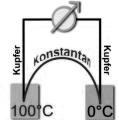
\includegraphics[width=0.15\textwidth]{Versuch_11-12/Abbildungen/Messung.JPG}
		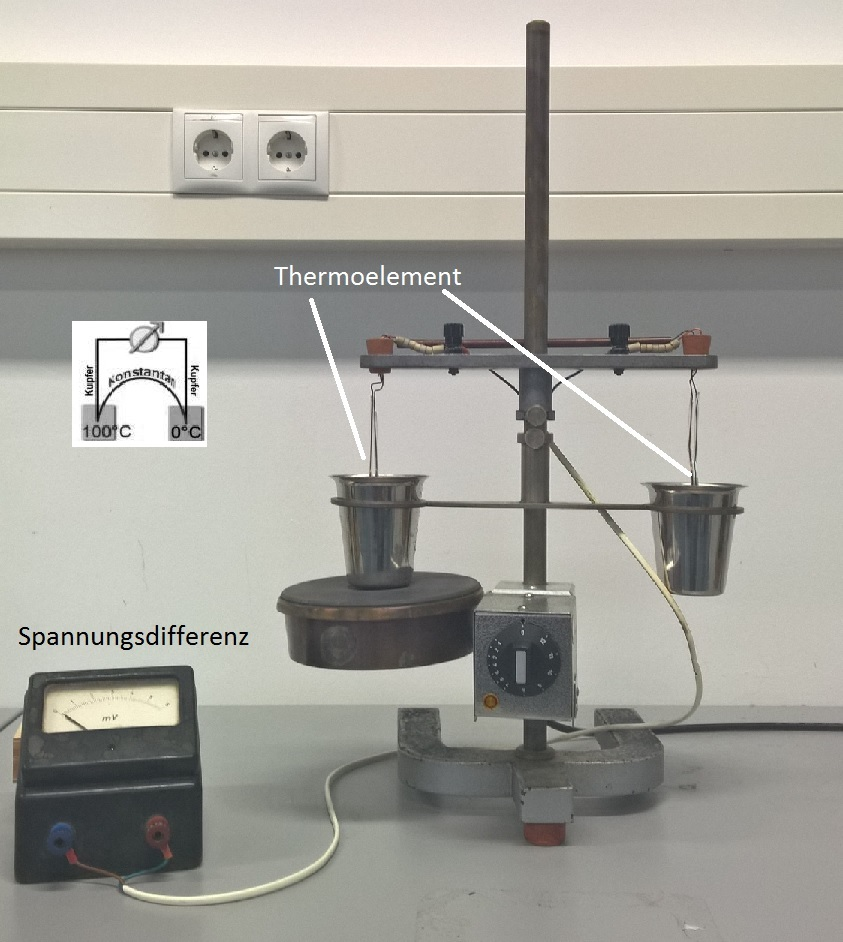
\includegraphics[width=0.75\textwidth]{Abbildungen/Thermoelement_Aufbau2.JPG}
	\caption{Messaufbau}
	\label{fig:Messung}
\end{figure}
%------------------------------------------------
\section{Auswertung} 
%------------------------------------------------
\etodo{Musterauswertung}

\begin{hint}
	Bitte fertigen Sie die Graphen in der folgenden Auswertung per Hand auf Millimeterpapier an.
\end{hint}

\begin{enumerate}
 %
 \item Stellen Sie die Thermospannung in mV als Funktion der Temperatur $T$ grafisch dar. Tragen Sie die Kurven f"ur Aufw"armung und Abk"uhlung des Wasserbades getrennt auf. \label{Aufg:a}
 %
 \item Lesen Sie aus der Auftragung die Empfindlichkeit des Thermoelementes ab. Sch"atzen Sie ihren Fehler aus den Grenzgeraden ab.\\
 Alle Geraden, auch die Grenzgeraden, m"ussen dabei durch den Ursprung gehen. Wieso?
 %
 \item Berechnen Sie den gewichteten Mittelwert der Empfindlichkeit des Thermoelementes. Die Formeln finden Sie im Skript.
 %
 \item Warum liegen die Geraden aus Aufgabe \ref{Aufg:a} nicht aufeinander?
 %
 \item Diskutieren Sie die Fehlerquellen in Ihrer Messung.
\end{enumerate}

\end{document}	% Thermoelement
%\chapter{Kennlinien verschiedener Leiter}
\label{v:12}

Die Kennlinie eines Leiter gibt an, wieviel Strom f"ur eine bestimmte angelegte Spannung durch diesen Leiter flie{\ss}t. In diesem Versuch werden Sie die Kennlinien einiger der meistgenutzten Leiter vermessen.

%------------------------------------------------
\section{Stichworte}
%------------------------------------------------

Spannung und Strom; Widerstand; Ohm'sche Gesetze; Temperaturabh"angigkeit von Widerst"anden; Leiter, Halbleiter und Isolatoren.

%------------------------------------------------
\section{Literatur}
%------------------------------------------------

Gehrtsen, Kapitel 6.1.2, 6.3.1 - 6.3.4, 6.4.3, 14.3.4, 14.4.1

%------------------------------------------------
\section{Anwendungsbeispiele}
%------------------------------------------------

So ähnlich wie das Thermoelement aus dem vorherigen Versuch werden temperaturempfindliche Widerstände zur schnellen Messung von Temperaturen benutzt. Einer der Vorteile gegenüber dem Thermoelement ist, dass diese auch als \textit{Widerstandsthermometer} bezeichneten Meßgeräte keine konstante Vergleichstemperatur brauchen.\\
Man kann hierzu Widerstände benutzen, bei denen der Widerstand mit der Temperatur steigt (\textit{Kaltleiter}, \textit{PTC}) oder fällt (\textit{Heißleiter, NTC})

%------------------------------------------------
\section{Theoretischer Hintergrund}
%------------------------------------------------

\subsection{Elektrischer Widerstand und das Ohm'sche Gesetz}

Bei allen Leitern gibt es einen Zusammenhang zwischen der Spannung $U$, die an den beiden Polen des Leiters angelegt wird, und der Stromst"arke $I$ des durch den Leiter flie{\ss}enden Stroms.
\begin{equation}\label{eq:Ohm}
U = R\cdot I \; .
\end{equation}
Den Proportionalit"atsfaktor $R$ nennt man den (ohmschen) \textit{Widerstand} des Leiters. \\
Ausser dem rein ohmschen Widerstand gibt es noch weitere Faktoren, zusammengefasst unter dem Begriff \textit{Impedanz}, die die Kennlinie $I=f(U)$ des Leiters beeinflussen. Diese wollen wir hier allerdings au{\ss}er Acht lassen (auch wenn ihre Behandlung sehr "ahnlich zu den ohmschen Widerst"anden ist).

\noindent
Bei einem homogenen ohmschen Material (Z. Bsp. ein St"uck Kupferdraht) ist der Widerstand $R$ proportional zur L"ange $l$ und umgekehrt proportional zum Querschnitt $A$ des Leiters:
\begin{equation}
R = \frac{\rho l}{A} \; .
\end{equation}
$\rho$ hei{\ss}t \textit{spezifischer Widerstand} des Materials.\\
Metalle leiten um so schlechter, je hei{\ss}er sie sind, bei Halbleitern ist es umgekehrt. F"ur kleinere Temperaturbereiche kann man eine lineare Temperaturbh"angigkeit des spezifischen Widerstandes annehmen:
\begin{equation}
\rho = \rho_0(1+\alpha T)\; .
\end{equation}
$\alpha$ hei{\ss}t Temperaturkoeffizient des Widerstandes. Er ist positiv f"ur Metalle (PTC- oder Kaltleiter) und negativ f"ur Halbleiter (NTC- oder Hei{\ss}leiter).

\subsection{Energie und Leistung elektrischer Str"ome}

Wenn sich eine Ladung $Q$ zwischen zwei Orten verschiebt, zwischen denen die Spannung $U$ herrscht, wenn sie also im Potenzial um $U$ absinkt, wird die Energie
 \begin{equation}
  W = Q\cdot U
 \end{equation}
frei. In Leitern geht diese Arbeit in die W"armeenergie des Leiters oder seiner Umgebung "uber. Die Leistung, welche den Leiter erhitzt, ergibt sich aus der Definition des Stroms:
 \begin{equation} \label{eq:Joule}
  P = \dot{W} = U\cdot\dot{Q} = U\cdot I \; .
 \end{equation}
Diesen Zusammenhang nennt man das \textit{Gesetz von Joule}.\\
F"ur einen ohmschen Leiter kann man, mit Gleichung \ref{eq:Ohm}, die Leistung auch schreiben als:
 \begin{equation}
  P = UI = I^2 R= \frac{U^2}{R}\; .
 \end{equation}

\subsection{Halbleiter, B"andermodell, etc.}

Wenn sich Atome in einem Kristallgitter befinden, nehmen sie einen sehr kleinen Abstand (wenige \AA) zueinander ein. Dann k"onnen die Elektronen "uber viele Atomabst"ande hinweg miteinander wechselwirken. Dies f"uhrt zu einer Aufweitung der (im Einzelatom noch als diskrete Niveaus vorliegenden) möglichen Energiewerte zu ausgedehnten Energiebereichen, den sogenannten Energiebändern. Da die Energiebänder je nach Aufweitung und Atomart verschieden zueinander liegen, können Bänder sich überlappen oder durch Energiebereiche, in der nach der Quantenmechanik keine erlaubten Zustände existieren (Energie- oder Bandlücke), getrennt sein. Das h"ochste besetzte Band wird \textit{Valenzband} genannt, das n"achsth"ohere Band hei{\ss}t \textit{Leitungsband}.\\
Die Fermienergie ist ein physikalischer Begriff aus der Quantenstatistik. Sie gibt die höchste Energie an, die ein Teilchen in einem Vielteilchensystem gleichartiger Fermionen (sog. Fermi-Gas) haben kann, wenn das System als Ganzes in seinem Grundzustand ist. Alle Zustände mit Energien zwischen dem tiefstmöglichen Niveau und der Fermi-Energie sind dann mit Teilchen voll besetzt, darüber keiner. Damit liegt das Ferminiveau also genau in der Bandl"ucke von Halbleitern.\\
Bei Halbleitern ist die Bandl"ucke relativ klein (Ge: $\approx 0,7$\,eV, Si: $\approx 1,1$\,eV, GaAs: $\approx 1,4$\,eV, Diamant: $\approx 5,4$\,eV). Daraus folgt, dass eine nicht zu vernachl"assigende Wahrscheinlichkeit besteht, durch thermische Anregung Elektronen ins Leitungsband anzuregen. Diese Wahrscheinlichkeit ist nat"urlich proportional zur Temperatur, d.h. f"ur h"ohere Temperaturen wird die Leitf"ahigkeit von Halbleitern besser, daher geh"oren sie zu den Hei{\ss}leitern.

\noindent
%Die relative Lage des h"ochsten besetzten Energiebandes (Valenzband) zum n"achsth"oheren Band (Leitungsband), in welchem sich die Elektronen frei durch den Festk"orper bewegen k"onnen, kann man benutzen, um Klassen von Materialien zu unterscheiden. \\
%Bei Leitern (z. Bsp. Metalle) "uberlappen das Valenzband und das Leitungsband, so dass sehr wenig Energie ben"otigt wird, um Elektronen vom Valenz- ins Leitungsband zu heben. Thermische Anregung (die kinetische Energie der Elektronen folgt der Maxwell-Verteilung) allein f"uhrt zu einer gro{\ss}en Anzahl beweglicher Elektronen.\\
%Bei Isolatoren ist die Bandl"ucke so gro{\ss} ($E_g > 4$\, eV), dass die Anzahl der Elektronen, die thermisch ins Leitungsband angeregt werden k"onnen, vernachl"assigbar ist, d.h. es gibt im wesentlichen keine beweglichen Elektronen im Festk"orper.\\
%Bei Halbleitern ist die Bandl"ucke relativ klein (Ge: $\approx 0,7$\,eV, Si: $\approx 1,1$\,eV, GaAs: $\approx 1,4$\,eV, Diamant: $\approx 5,4$\,eV).

%------------------------------------------------
\section{Fragen zur Vorbereitung}
%------------------------------------------------

\begin{enumerate}
 %
 %\item Was soll heute im Praktikum gemessen werden? Warum?
 %%
 \item Wie sind Strom und Spannung definiert? (Erkl"aren Sie: $U_{12} = - \int_{1}^{2}{\vec{E}d\vec{r}}$)
 %
 \item Wie ist der elektrische (ohmsche) Widerstand definiert?
 %
 \item Wie h"angt der elektrische Widerstand von den r"aumlichen Dimensionen des Leiters und vom Material ab?
 %
 \item Was mi{\ss}t ein Ampere-/Voltmeter? Wie wird es in den Stromkreis geschaltet?
 %
 %\item Erkl"aren Sie das B"andermodell eines Halbleiters. (Definition: Valenzband, Leitungsband, Ferminiveau)\\
 % Warum kann ein volles Band keinen Strom leiten?
 %
 \item Wie sieht die Bandstruktur eines Isolators, Halbleiters und Leiters aus? Skizze.
 %
 \item Erl"autern Sie die Temperaturabh"angigkeit des spezifischen Widerstandes $\rho$.
 %
 \item Warum (und wie) verändert sich der Widerstand eines Leiters (Metall) bei Veränderung der Temperatur? Was bedeuten PTC und NTC?
 %
 \item Warum ist das Verhalten von Halbleitern bei Temperaturveränderung entgegengesetzt dem von Leitern ? Erklärung mit Bändermodell.
 %
 \item Wie funktioniert eine Spannungsteilerschaltung?
 %
\end{enumerate}

%------------------------------------------------
\section{Durchführung} 
%------------------------------------------------

\begin{enumerate}
 %
 \item Messen Sie f"ur die Metallfadenlampe die Stromst"arke $I$ als Funktion der angelegten Spannung $U$.\\
  Fahren Sie dazu die Spannung $U$ in Schritten von 1\,V von 0\,V bis 12\,V hoch und lesen Sie die Stromst"arke $I(U)$ ab.\\
  In diesem Versuchsteil wird das Thermoelement nicht angeschlossen.
\end{enumerate}
Benutzen Sie zur Messung der Kennlinien die folgende Schaltung:
\begin{figure}[h]
	\centering
		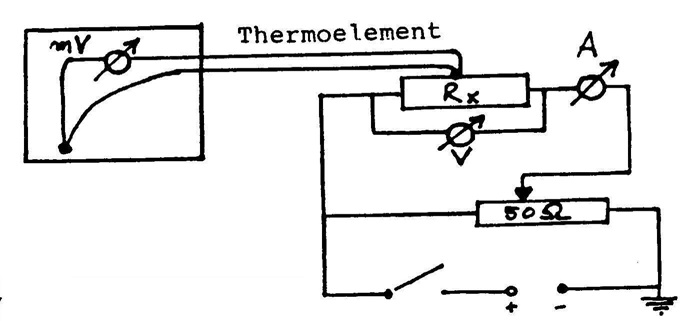
\includegraphics[width=.5\textwidth]{Versuch_11-12/Abbildungen/Schaltplan-12.jpg}
	\label{fig:Schaltplan-12}
\end{figure}

\begin{enumerate} \setcounter{enumi}{1}
 %
 \item Die NTC und PTC Widerst"ande erw"armen sich signifikant, wenn Strom durch sie flie{\ss}t. Schliessen Sie daher f"ur die Messung ihrer Kennlinien das Thermoelement direkt an die schwarzen Buchsen an. Das Thermoelement darf nicht mit dem restlichen Stromkreis verbunden sein.
 %
 \item Messen Sie f"ur den NTC und den PTC den Widerstand als Funktion der Temperatur des Bauteils.\\
  Warten Sie nach jeder Einstellungs"anderung, bis sich der Strom $I$ bei eingestellter Spannung $U$ nicht mehr "andert (ca. 1 min). Lesen Sie erst dann Strom, Spannung und Thermospannung ab.
  \begin{itemize}
   %
   \item Stellen Sie f"ur den PTC Spannungen von 0-12\,V in 1\,V-Schritten ein.
   %
   \item F"ur den NTC ver"andern Sie die Stromst"arke: Beginnen Sie bei einer hohen Stromst"arke von 300\,mA und gehen Sie in 30\,mA-Schritten herunter bis 0\,mA.
   
    \noindent
    \textbf{Achtung:} Achten Sie darauf, dass durch den NTC nie mehr als 300\,mA flie{\ss}en!\\
    Drehen Sie dazu den Strom zun"achst voll auf. Ab ca. 150\,mA steigt die Stromst"arke sehr schnell an. Regeln Sie dann den Strom entsprechend runter. Beobachten Sie die Messger"ate w"ahrend dieses Vorganges sehr genau!\\
    Lassen Sie den NTC bei eingestelltem Strom ins thermische Gleichgewicht zur"uckkehren, bevor Sie ihre Messung starten.
   %
  \end{itemize}
 %
 \item Messen Sie die Raumtemperatur.
 %
\end{enumerate}

%------------------------------------------------
\section{Auswertung} 
%------------------------------------------------

\begin{enumerate}
 %
 \item Stellen Sie die Kennlinie der Metallfadenlampe, $I=f(U)$, grafisch dar.
 %
 \item Grafische Darstellung des Widerstandes des NTC- und des PTC-Leiters als Funktion der Temperatur.
  \begin{itemize}
   \item Berechnen Sie aus der Thermospannung die Temperatur wie folgt.\\
    Im Idealfall betr"agt die Thermospannung bei Raumtemperatur 0\,V. Wenn dem nicht so ist, ziehen Sie von ihren Messwerten die bei Raumtemperatur gemessenen Thermospannung $U_{th}(RT)$ ab. Die Eichung des Thermoelementes betr"agt $a = 54\,\mu V / ^{\circ}C$. Damit errechnet sich die Temperatur in $^{\circ}C$ zu:
    \begin{equation}
     T = \frac{U_{th}(T) - U_{th}(RT)}{a} + RT
    \end{equation}
   %
   \item Berechnen Sie aus den U und I Wertepaaren den Widerstand des Leiters.
   %
   \item Tragen Sie f"ur den NTC-Leiter den nat"urlichen Logarithmus des Widerstandes $\ln(R)$ als Funktion von $1/T$ auf. Benutzen Sie die Temperatur in Kelvin.\\
    Da die Temperaturabh"angigkeit eines Hei{\ss}leiters einem Exponentialgesetz folgt:
    \begin{equation}
     R(T) = A\cdot \exp\left(\frac{\Delta E}{2k_b T}\right)
    \end{equation}
    ergibt diese Auftragung eine Gerade. Die Konstante $A$ h"angt von Bauform und Material des Hei{\ss}leiters ab.\\
    Berechnen Sie aus der Steigung der Geraden die Energiel"ucke $\Delta E$ zwischen Valenz- und Leitungsband des Halbleitermaterials, aus dem der Hei{\ss}leiter aufgebaut ist. Berechnen Sie den Fehler von $\Delta E$ aus der bekannten Fehlerfortpflanzung.
    
    \noindent
    Hinweis: $k_b = 8,62 \times 10^{-5}$\, eV/K
  \end{itemize}
 %
 \item Vergleichen Sie die gemessene Energiel"ucke mit Literaturwerten und diskutieren Sie die Fehlerquellen in Ihrer Messung.
 %
\end{enumerate}	% Kennlinien verschiedener Leiter
\chapter{Ultraschall}
\label{vn:2}

In diesem Versuch werden Eigenschaften der Ausbreitung von Wellen in Medien anhand einiger Anwendungen von Ultraschall untersucht.
%
%------------------------------------------------
\section{Stichworte}
%------------------------------------------------
Ultraschall, Ausbreitung von Wellen, Longitudinal- und Transversalwellen, Reflexion und Transmission, Beugung, Totalreflexion.
%
%------------------------------------------------
\section{Literatur}
%------------------------------------------------
Gehrtsen, Kapitel 3.4, 4.2.1-3; Demtröder, Kapitel 11.9
%
%------------------------------------------------
\section{Anwendungsbeispiele}
%------------------------------------------------
%
Elastische Wellen mit Frequenzen oberhalb der menschlischen Hörschwelle (15 bis 20~kHz) bis etwa 10~GHz nennt man \textit{Ultraschall}. Bei großen Frequenzen liegen die Wellenlängen im selben Bereich wie die von sichtbaren Licht, weshalb Beugungserscheinungen, die die Ausbreitung des hörbaren Schalls so komplizieren, an Bedeutung verlieren. Das Schallfeld kann sehr gut fokussiert werden und kann so zur Ortung und Hinderniserkennung durch Richtstrahlreflexion genutzt werden (z. Bsp. Sonar in der Schifffahrt, bei Fledermäusen und Delphinen). \\
In Materialien mit einfachem Molekülaufbau, z. Bsp. in Metallen ist die Absorption von Ultraschall sehr gering. Daher und wegen seiner Ungefährlichkeit im Vergleich mit anderen Strahlungsarten (Röntgen, hartes UV-Licht, Neutronen), wird Ultraschall wird Ultraschall in vielen Bereichen benutzt: Ultraschallechografie in Medizin, Werkstoffprüfung, Dickenmessung, externe Messung des Füllstandes von Tanks, Konzentrationsmessung in Lösungen. Die Untersuchung der Ausbreitung von longitudinalen und transversalen Erdbebenwellen erlaubt detaillierte Untersuchungen der Erdkruste, erbrachte die ersten Hinweise auf die flüssige Natur des Erdmantels und erlaubt die Triangulation der Epizentren von Erdbeben.
%
%------------------------------------------------
\section{Theoretischer Hintergrund}
%------------------------------------------------

%Schallwellen, die sich in einem Medium ausbreiten, verursachen eine zeitlich und räumlich periodische Änderung von Dichte, Druck und Temperatur. Man kann die Ausbreitung der Welle in jeder dieser Größen darstellen, wir entscheiden uns hier für die Darstellung durch den zeitlichen und räumlichen Verlauf des Druckes $p = p(x,t)$.
\subsection{Deformation von Festkörpern}

Das Verhalten von Festkörpern unter Deformation ist recht kompliziert und mathematisch sehr anspruchsvoll. Da wir allerdings einige der Zusammenhänge brauchen, um die Ausbreitung von Wellen in Fluiden und Festkörpern zu verstehen, seien sie hier knapp zusammengefasst.

\subsubsection{Dehnung und Kompression}

Eine Kraft $F$, die an einem Draht mit der Querschnittsfläche $A$ zieht, verlängert diesen um ein Stück $\Delta l$. Bei nicht zu großer Kraft $F$ ist diese Verlängerung proportional zu $F$, zur Drahtlänge $l$ und zu $1/A$. Betrachten wir die relative Längenänderung $\epsilon = \Delta l/l$, so ergibt sich dieses \textit{Hooke'sche Gesetz}:
\begin{equation}
	\epsilon=\frac{1}{E}\sigma\; ,
\end{equation}
mit der \textit{Zugspannung} $\sigma=F/A$.\\
Die Proportionalitätskonstante $E$ heißt \textit{Elastizitätsmodul} und hat die Einheit N/m$^2$.\\
Ein Draht, an dem man zieht, wird nicht nur länger sondern gleichzeitig auch dünner. Sein Durchmesser $d$ nehme $\Delta d < 0$ ab. Dann bezeichnet man das Verhältnis der beiden relativen Deformationen als \textit{Poisson-Zahl} $\mu$:
\begin{equation}
	\mu = \frac{\Delta d}{d}\frac{l}{\Delta l}\; .
\end{equation}
Wirkt in allen drei Raumrichtung gleichzeitig eine Zugspannung auf einen Körper, so ändert sich dessen Volumen um
\begin{equation}
	\frac{\Delta V}{V} = \frac{3 \sigma}{E}\left( 1-2\mu\right) = \kappa\sigma
\end{equation}
mit der \textit{Kompressibilität} $\kappa$.

\subsubsection{Scherung}

\begin{minipage}[b]{0.64\textwidth}
Eine Kraft $F$, die tangential zu einer Fläche $A$ wirkt bezeichnet man als \textit{Scherkraft}. Diese kippt alle zu $A$ senkrechten Kanten eines Quaders um den Winkel $\alpha$, der proportional zur Kraft und zur Fläche $A$ ist, solange die Deformation nicht zu groß wird:
\begin{equation}
	\tau = \frac{F}{A} = G\cdot \alpha\; .
\end{equation}
Die Proportionalitätskonstante $G$ heißt \textit{Torsionsmodul} oder \textit{Schubmodul}.
\end{minipage}
\hfill
\begin{minipage}[b]{0.30\textwidth}
	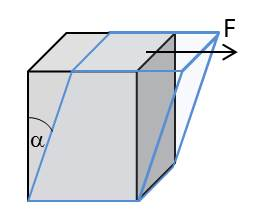
\includegraphics[width=.8\textwidth]{Versuch_neu_1-2/figures/Scherung.jpg}
	\captionof{figure}{Deformation eines Würfels durch Scherkräfte}
	\label{fig:Scherung}
\end{minipage}


\subsection{Beschreibung von Wellen}

Spannen wir ein Seil zwischen zwei Punkten fest ein und schlagen nahe eines der Enden (am Ort $x_0$) kurz darauf, so entsteht eine Auslenkung, die über die ganze Länge des Seils bis zum anderen Ende läuft, dort reflektiert wird und zurückläuft. So kann die Auslenkung mehrmals über das Seil hin- und herlaufen, ohne ihre Form stark zu ändern. Diese Form von Seilwellen kennen Sie aus dem Alltag von der Schwingung einer Saite oder, in zwei Dimensionen, als Ausbreitung einer Oberflächenwelle in Wasser.\\
Wir bezeichnen die Auslenkung $y$ des Seils am Ort $x$ und zur Zeit $t$ mit $y=f(x,t)$. Die ursprüngliche Auslenkung $f(x_0, 0)$ soll nach der Zeit $t$ um die Strecke $ct$ gewandert sein, $c$ bezeichnet also die Ausbreitungsgeschwindigkeit der Welle.\\
Ein undehnbares Seil können wir nur senkrecht zu seiner Richtung auslenken und so eine \textit{Transversalwelle} erzeugen. Bei einem dehnbaren Seil, oder äquivalent einer Schraubenfeder, können wir auch eine Auslenkung entlang der Richtung des Seils erzeugen, die sich dann als \textit{Longitudinalwelle} fortpflanzt.\\

\noindent
Betrachten Wir einen Punkt auf dem Seil als Funktion der Zeit, so führt dieser eine Schwingung um die Ruhelage aus, wie wir sie in Versuch \ref{vn:1} kennengelernt haben. Wie wir wissen kommt eine Schwingung zustande, wenn es eine der Auslenkung proportionale Rückstellkraft gibt, welche in Richtung der Ruhelage wirkt.\\
Mit der Zugspannung $\sigma$ können wir eine Wellengleichung aufstellen
\begin{equation*}
	\frac{d^2 y}{dt^2} = c^2\frac{d^2 y}{dx^2}\quad \mathrm{mit}\quad c^2 = \frac{\sigma}{\rho}\; .
\end{equation*}

\subsubsection{Schallgeschwindigkeit in Medien}

Eine ähnliche Wellengleichung kann man auch für den Fall elastischer Wellen in Festkörpern oder Flüssigkeiten aufstellen. Diese stellen wir als zeitlich und räumlich periodische Änderungen des Drucks des Mediums dar:
\begin{equation*}
	\ddot{p} = \frac{1}{\kappa\rho} p''\; ,
\end{equation*}
mit der Dichte $\rho$ des Mediums. Ist das Medium ein Festkörper ersetzen wir die Kompressibilität durch den Kehrwert des Elastizitätsmoduls und finden für die Geschwindigkeit dieser longitudinalen Schallwelle:
\begin{equation}
	c_{long} = \sqrt{\frac{1}{\kappa\rho}} = \sqrt{\frac{E}{\rho}}\; .
\end{equation}

\subsubsection{Transversale Schallwellen}

Trifft eine longitudinale Schallwelle auf die Oberfläche eines Festkörpers und wird in diesen hinein transmittiert, so regt sie (vereinfachend dargestellt) die Atome des Festkörpers zu einer Schwingung entlang der Ausbreitungsrichtung der Welle und damit senkrecht zur Oberfläche des Festkörpers an. Diese Atome sind elastisch mit ihren Nachbarn gekoppelt, so dass diese ebenfalls zu Schwingungen angeregt werden. Betrachten wir diesen Vorgang als eine Verschiebung von Schichten des Festkörpers, die senkrecht zur Oberfläche stehen, so kann man aus diesen einen Quader zusammensetzen, der als ganzes durch die einlaufende Schallwelle in Form einer Scherung deformiert wird. \\
Es entsteht eine Welle, bei der die Atome senkrecht zur Bewegungsrichtung schwingen, also eine Transversalwelle. Mit den obigen Überlegungen überrascht es nicht, dass die Schallgeschwindigkeit dieser Transversalwelle durch das Schermodul bestimmt wird, anstelle des Elastizitätsmoduls, wie bei Longitudinalwellen:
\begin{equation}
	c_{trans} = \sqrt{\frac{G}{\rho}}\; .
\end{equation}
In Festkörpern, und nur in diesen, können sich also transversale Schallwellen ausbreiten, die Geschwindigkeit nicht gleich der Geschwindigkeit von Longitudinalwellen sind. Tabelle \ref{tab:Schallgeschwindigkeiten} zeigt einige Beispielwerte.

\begin{table}[hb]
	\centering
		\begin{tabular}{l|l|l}
			Material & $c_{long}$/ms$^{-1}$ & $c_{trans}$/ms$^{-1}$ \\
			\hline
			Aluminium & 6420 & 3020\\
			Blei & 1960 & 690\\
			Flintglas & 3980 & 2380\\
			Polyacryl & 2610 & 1430\\
		\end{tabular}
	\caption{Schallgeschwindigkeiten für longitudinale und transversale Wellenausbreitung in verschiedenen Festkörpern bei 20\degree~C.}
	\label{tab:Schallgeschwindigkeiten}
\end{table}

Mit Hilfe einer etwas komplizierten Rechnung, die wir hier nicht vormachen wollen, kann man zeigen, dass die Amplitude der transmittierten Transversalwelle maximal wird, wenn sie sich im Festkörper unter einem Winkel von etwa 45\degree zur Oberflächennormalen ausbreitet. Im wohlbekannten Bild der Brechung einer Welle an einer Oberfläche (s. Versuch \ref{v:9}) ist das der Ausfallswinkel nach der Brechung. Nach dem Snellius'schen Brechungsgesetz gilt dann für den Einfallswinkel $\alpha$
\begin{equation}
	\frac{c_{trans}}{c_0} = \frac{\sin 45\degree}{\sin \alpha}\; ,
\end{equation}
wobei $c_0$ die Schallgeschwindigkeit in der umgebenden Flüssigkeit sei.\\
Damit wird der Einfallswinkel, unter dem die Amplitude der Transversalwelle maximal ist
\begin{equation}
	\sin \alpha_{max} = \frac{c_0}{c_{trans}} \sin 45\degree = \frac{c_0}{\sqrt{2}c_{trans}}\; .
\end{equation}
Wie bei der Brechung von Licht, kann der Ausfallswinkel $\beta = 90\degree$ werden, was der Totalreflektion der Transversalwelle entspricht. Für den Einfallswinkel gilt dann
\begin{equation}
	\sin \alpha_{tot} = \frac{c_0}{c_{trans}} \sin 90\degree = \frac{c_0}{c_{trans}}\; .
\end{equation}

\subsection{Erzeugung und Empfang von Ultraschall}

Bestimmte kristalline Stoffe sind in der Lage, einen mechanischen Druck in eine elektrische Spannung und umgekehrt eine elektrische Spannung in eine mechanische Deformation umzuwandeln. Diese Fähigkeit nennt man Piezoelektrizität.\\

\noindent
Ein Ultraschallwandler besteht aus einer Scheibe aus piezoelektrischem Material, deren Stirnflächen mit einer elektrisch leitfähigen Schicht überzogen sind. Legt man an die Stirnflächen eine elektrische Spannung, so entsteht zwischen ihnen ein elektrisches Feld. Das elektrische Feld übt eine Kraft auf die Gitterbausteine aus. Aufgrund vorhandener Unsymmetrien des aus positiven und negativen Ionen aufgebauten Gitters wirkt sich die Polarität des äußeren Feldes entweder verstärkend oder schwächend auf die Bindungskräfte innerhalb des Kristalls aus. Eine Verstärkung bedingt ein Zusammenziehen (Kontraktion), während eine Schwächung eine Ausdehnung (Dilatation) des Kristalls zu Folge hat. Die Frequenz, mit der die Scheibe kontrahiert und dilatiert, wird durch die angelegte Wechselspannung festgelegt.\\

\noindent
Der Piezokristall ist ein Oszillator, der durch die elektrische Wechselspannung zu erzwungenen Schwingungen angeregt wird. Dadurch hat er naturgemäß eine bestimmte Resonanzfrequenz, in welcher die Schwingungsamplitude und damit die abgestrahlte Intensität maximal sind. Die Resonanz hängt ab vom Material und den Dimensionen des Sender-Kristalls. Aus diesem Grund ist es notwendig, für jede gewünschte Ultraschallfrequenz einen speziell für diesen Zweck konstruierten Wandler zur Verfügung zu haben. Der Piezoeffekt ist umkehrbar. Derselbe Kristall kann daher sowohl als Sender, wie oben beschrieben, als auch als Empfänger genutzt werden. Die auf den Schallkopf auftreffenden Schallwellen, bzw. die Druckschwankungen am Ort des Schallkopfes, regen diesen zu mechanischen Schwingungen an, die sich an den Stirnflächen des Kristalls als elektrische Wechselspannung registrieren lassen.

\subsection{Anwendung: Sonographie}

Innerhalb der letzten 30 Jahre hat sich die Sonographie zu einer sehr wirkungsvollen Methode im Bereich der nichtinvasiven Diagnostik entwickelt. Man denke hier nur an die Schwangerschafts-Vorsorge oder die Funktionsdiagnostik in der Kardiologie. Das einfachste und zugleich älteste Verfahren ist das dem Echolot-Prinzip folgende A-Bild (A-Scan). Das A-Bild-Verfahren findet Anwendung in der Untersuchung des Auges, z.B. auf das Vorliegen einer Netzhautablösung und ist darüber hinaus die Grundlage aller anderen Ultraschall-Techniken.\\

\noindent
Im Folgenden soll das Grundprinzip des A-Bild-Verfahrens beschrieben werden: Der Schallsender gibt kurze Schallimpulse ab. Nach jedem Impuls wird der Sender abgeschaltet und arbeitet bis zum nächsten Impuls als Empfänger. Trifft der Impuls auf ein Objekt oder eine Grenzfläche, wird er dort ganz oder teilweise reflektiert.\\
Der reflektierte Impuls erreicht nach einer Zeit, die der doppelten Laufzeit (Hin- und Rückweg) zwischen dem Objekt und dem Schallkopf entspricht, den Empfänger und löst dort ein elektrisches Signal aus. Dessen Amplitude ist proportional zur Intensität des zurückgelangten Signals.\\
Man trägt nun in einem Diagramm die Stärke (Amplitude) des Echosignals über der Zeit auf, die seit dem Aussenden des Pulses vergangen ist. Diese Darstellung wird als A-Bild (Amplitude-Bild) bezeichnet. Für jeden neuen Sendepuls beginnt das Bild wieder neu (synchronisiert). Das dargestellte Zeitfenster wird so eingestellt, dass die reflektierten Signale aus den tiefsten darzustellenden Schichten innerhalb dieser Zeit am Empfänger eintreffen. Für den zeitlichen Abstand zwischen den Sender-Impulsen gilt darüber hinaus, dass er länger sein muss als die maximale Laufzeit eines Reflex-Signals. Jedes detektierte Echosignal erzeugt also im Empfänger eine elektrische Spannung, die nun verstärkt in $y$-Richtung über der Zeit ($x$-Achse) dargestellt wird. Die elektrische Verstärkung kann für längere Laufzeiten vergrößert werden, um die Verluste auf den längeren Laufwegen annähernd gleichmäßig zu kompensieren.\\

\noindent
Aus der Laufzeit $\Delta t$ des Reflex-Signals lässt sich über die Beziehung
\begin{equation*}
	\Delta s = c\cdot \Delta t
\end{equation*}
der doppelte Laufweg $\Delta s$ des Signals bestimmen.\\
Die Schallgeschwindigkeiten der verschiedenen Gewebearten (außer Knochen) sind annähernd gleich. Dies erlaubt es, die $x-$Achse mit einer Skala zu versehen, auf der jeder $x-$Wert einer bestimmten Tiefe des durchstrahlten Objektes entspricht. Aus dem Abstand zweier $y-$Auslenkungen ist dann direkt der Abstand der Schichten abzulesen, an denen der Schallimpuls reflektiert wurde.\\

\noindent
Eine übliche Erweiterung der Darstellungsform ist die Auftragung der reflektierten Amplitude als Helligkeit (Grauwert). Dadurch reduziert sich das Zeit-Amplituden-Diagramm ($x-y$-Diagramm, A-Scan) auf eine Linie mit verschieden hellen Punkten. Man kann nun viele solche Linien nebeneinander auftragen und erhält ein zweidimensionales Grauwertebild. In der Regel wird dabei die Eindringtiefe (bzw. Zeitachse) von oben vertikal nach unten angezeigt. Bildet man zeitlich aufeinander folgende A-Scans derart von links nach rechts ab, erhält man den sog. TM-Scan
(time mode).\\
Eine wichtige Anwendung des TM-Scans ist das Herzecho. Man schaut hier auf die Wanddicke des Herzens und deren Veränderung während des Schlagens. Daran lassen sich z.B. Klappenfehler und Herzinsuffizienzen erkennen.\\

\noindent
Um auch in Querrichtung Informationen zu erhalten, lässt man den Schallkopf nicht nur einmal den Schall aussenden und wieder einfangen, sondern scannt in verschiedenen Winkeln die Körperstrukturen ab. Die aneinandergesetzten A-Scan-Linien entsprechen nun verschiedenen Durchstrahlrichtungen und das Bild zeigt eine Schnittebene durch den Körper. Diese Darstellung heißt B-Bild oder B-Scan (von
brightness).

%------------------------------------------------
\section{Fragen zur Vorbereitung}
%------------------------------------------------

\begin{enumerate} 
	\item Welche Deformation eines Festkörpers wird durch das Elastizitätsmodul beschrieben? Welche durch das Schubmodul? Geben Sie an, in welche Richtung jeweils die Kraft wirkt.
	%
	\item Wie groß ist die Schallgeschwindigkeit in Luft ungefähr?
	%
	\item Wieso treten transversale Schallwellen ausschließlich in Festkörpern auf und nicht in Fluiden?
\end{enumerate} 

%------------------------------------------------
\section{Durchführung} 
%------------------------------------------------

\subsection{Vorbereitung}

Schließen Sie die beiden Ultraschallsonden an den \verb RECEIVER  bzw. \verb TRANSMITTER -Ausgang des Betriebsgeräts an.
Auf dem PC als Benutzer \verb prakt  einloggen (kein Passwort), das Betriebsgerät anschalten und auf dem PC das Programm \verb AScan  starten. Im oberen Teil der Anzeige ist der Zeitverlauf der Amplitude des empfangenen Signals zu sehen, im unteren der Zeitverlauf der Verstärkung. Unter \verb RECEIVER  kann zwischen \verb REFLECT.  und \verb TRANS. , also reflektiertem bzw. transmittiertem Signal an Hand der Laufzeit unterschieden werden. Auf transmittiertes Signal stellen. \\
In der Menüleiste des Programms auf die volle Zeitachse stellen (der Knopf neben Stop sollte \verb Half  anzeigen, ansonsten \verb Full  drücken). Eine Bedienungsanleitung des Steuergeräts befindet sich auf dem Desktop unter dem Icon \verb AScan  Handbuch.

\subsection{Durchführung}

\begin{enumerate}
	%%%%%%%%%%%%%%%%%%%%%%%%%%%%%%%%%%%%%%%%%%%%%%%%%%%%%%%%%%%%%%%%%%%%%%%%%%%%%%%%%%%%%%%%%%%%%%%%%%%%
	% Teil 1
	%%%%%%%%%%%%%%%%%%%%%%%%%%%%%%%%%%%%%%%%%%%%%%%%%%%%%%%%%%%%%%%%%%%%%%%%%%%%%%%%%%%%%%%%%%%%%%%%%%%%
	\item \textbf{Schallgeschwindigkeit als Funktion der Temperatur}
	\begin{enumerate}
		\item Füllen Sie die große Wanne zu etwa einem Drittel mit Leitungswasser und fügen Sie Eis hinzu. Mischen Sie so lange, bis das Wasser eine Temperatur von 0\degree C hat und keine Eiskristalle mehr darin schwimmen. \textbf{Das ist sehr wichtig, da diese die Pumpe des Durchlauferhitzers beschädigen können.}
		%
		\item Platzieren Sie den Ultraschallsender und -empfänger so, dass eine unbehinderte Sichtlinie zwischen den beiden besteht. Vergessen Sie nicht, das Ultraschall-Übertragungsgel zu verwenden.\\
		Stellen Sie die Verstärkung am Betriebsgerät unter \verb RECEIVER  auf den kleinsten Wert und stellen Sie die Ausgangsleistung unter \verb TRANSMITTER  so ein, dass das empfangene Signal gut erkennbar ist und unter 1,2V liegt, da ansonsten der Verstärker in Sättigung geht.
		%
		\item Messen Sie den Abstand zwischen den beiden Sonden.
		%
		\item Messen Sie die Laufzeit des Ultraschallpulses bei etwa 0\degree C mit Hilfe des ersten Cursors. Wie genau ist die Zeitmessung?
	\end{enumerate}
	%
	Für die nun folgende Messung der Schallgeschwindigkeit als Funktion der Temperatur empfiehlt es sich, das ein Praktikant den PC bedient und der/die andere die Temperatur im Auge behält und die Messwerte notiert. Zur Messung der Änderung der Laufzeit des Ultraschallpulses empfiehlt es sich, den ersten Cursor bei der ursprünglichen Laufzeit zu lassen und mit dem zweiten Cursor die neue Laufzeit zu messen. Das Programm berechnet automatisch die Differenz der beiden Zeiten in $\mu$s.
	%
	\begin{enumerate} \setcounter{enumii}{3}
		%
		\item Starten Sie den Lauda Durchlauferhitzer. Stellen Sie die Solltemperatur auf 35\degree C. Der Durchlauferhitzer fängt sofort an, das Wasser aufzuheizen, behalten Sie daher die Anzeige der Isttemperatur im Auge.
		%
		\item Messen Sie die Laufzeitdifferenz des Ultraschallpulses als Funktion der Temperatur in Schritten von etwa 2\degree. Schätzen Sie die Unsicherheit der Temperaturmessung ab.
	\end{enumerate}
	%
	%%%%%%%%%%%%%%%%%%%%%%%%%%%%%%%%%%%%%%%%%%%%%%%%%%%%%%%%%%%%%%%%%%%%%%%%%%%%%%%%%%%%%%%%%%%%%%%%%%%%
	% Teil 2
	%%%%%%%%%%%%%%%%%%%%%%%%%%%%%%%%%%%%%%%%%%%%%%%%%%%%%%%%%%%%%%%%%%%%%%%%%%%%%%%%%%%%%%%%%%%%%%%%%%%%
	\item \textbf{Schallgeschwindigkeit als Funktion der Salzkonzentration}
	\begin{enumerate}
		\item Füllen Sie die kleine Wanne mit Leitungswasser, so dass die beiden an der Längsseite außen angebrachten Sonden vollständig bedeckt sind (für die Anbringung das Ultraschall-Übertragungsgel verwenden). Benutzen Sie hierfür den Messbecher und notieren Sie das Volumen des Wassers, da Sie dieses zur Berechnung der Salzkonzentration brauchen.
		%
		\item Messen Sie die Laufzeit des Ultraschallpulses in Leitungswasser mit dem 1. Cursor.
		%
		\item Stellen Sie nun mit dem Kochsalz Lösungen von 25, 50, 75, 100, 150, 200, 250~g/l her und messen Sie jeweils die Laufzeitdifferenz des Ultraschallpulses mit Hilfe des zweiten Cursors. Bevor Sie die  Messung durchführen können müssen die Salzkristalle komplett gelöst sein. Wieso ist das so?\\ 
		Schätzen Sie die Unsicherheit der Kochsalzkonzentration Ihrer Lösung ab.
	\end{enumerate}
	%%%%%%%%%%%%%%%%%%%%%%%%%%%%%%%%%%%%%%%%%%%%%%%%%%%%%%%%%%%%%%%%%%%%%%%%%%%%%%%
	% Teil 3: Alternativ für Geowissenschaftler
	%%%%%%%%%%%%%%%%%%%%%%%%%%%%%%%%%%%%%%%%%%%%%%%%%%%%%%%%%%%%%%%%%%%%%%%%%%%%%%%
	\item \textbf{Für Geowissenschaftler: \\
		Longitudinale und transversale Schallwellen in Festkörpern}
	\begin{enumerate}
		\item Platzieren Sie die Polyacrylplatte in die Mitte des Beckens und stellen den Knopf auf 20\degree .\\
		Es sollte nun zwei Signale, ggf. mit einem ''Satelliten'' zu sehen sein (durch Mehrfachreflexion, diese ignorieren): das frühere Signal entspricht wegen der etwa zweifach größeren Schallgeschwindigkeit der longitudinalen Schallwelle, das spätere entsprechend der transversalen Welle. Messen Sie die Amplitude beider Signale mit dem hellblauen Cursor im \verb AScan -Programm als Funktion des Auftreffwinkels in Schritten von 5\degree~zwischen 0\degree~und 90\degree; ggf. während der Messung die Verstärkung erhöhen.
		%
		\item Wiederholen Sie diese Messung analog mit der Aluminiumplatte.
	\end{enumerate}
	%
\end{enumerate}


%------------------------------------------------
\section{Auswertung} 
%------------------------------------------------

\begin{enumerate}
	%%%%%%%%%%%%%%%%%%%%%%%%%%%%%%%%%%%%%%%%%%%%%%%%%%%%%%%%%%%%%%%%%%%%%%%%%%%%%%%%%%%%%%%%%%%%%%%%%%%%
	% Teil 1
	%%%%%%%%%%%%%%%%%%%%%%%%%%%%%%%%%%%%%%%%%%%%%%%%%%%%%%%%%%%%%%%%%%%%%%%%%%%%%%%%%%%%%%%%%%%%%%%%%%%%
	\item\textbf{Schallgeschwindigkeit als Funktion der Temperatur}
	\begin{enumerate}
		\item Berechnen und tabellieren Sie die Laufzeiten der Ultraschallpulse als Funktion der Temperatur aus dem Wert bei 0\degree~C und den gemessenen Laufzeitunterschieden.
		%
		\item Berechnen Sie aus dem gemessenen Abstand zwischen Ultraschallsender und -empfänger, sowie aus den Laufzeiten der Pulse die Schallgeschwindigkeit in Wasser als Funktion der Temperatur. Wie groß ist die Unsicherheit der Werte?
		%
		\item Tragen Sie die berechneten Schallgeschwindigkeiten gegen die Temperatur auf. Beachten Sie, dass sowohl die Schallgeschwindigkeit, wie auch die Temperatur bei der sie gemessen wurde Unsicherheiten haben.
		%
		\item Die Schallgeschwindigkeit in Leitungswasser sollte bei Raumtemperatur $c=1480$~m/s betragen. Stimmt diese Angabe mit Ihren Messwerten überein? Wenn nicht, warum nicht?
	\end{enumerate}
	%
	%%%%%%%%%%%%%%%%%%%%%%%%%%%%%%%%%%%%%%%%%%%%%%%%%%%%%%%%%%%%%%%%%%%%%%%%%%%%%%%%%%%%%%%%%%%%%%%%%%%%
	% Teil 2
	%%%%%%%%%%%%%%%%%%%%%%%%%%%%%%%%%%%%%%%%%%%%%%%%%%%%%%%%%%%%%%%%%%%%%%%%%%%%%%%%%%%%%%%%%%%%%%%%%%%%
	\item \textbf{Schallgeschwindigkeit als Funktion der Salzkonzentration}
	\begin{enumerate}
		\item Die Schallgeschwindigkeit in Leitungswasser beträgt bei Raumtemperatur $c~=~1480$~m/s. Für die Schallgeschwindigkeit bei einer gegebenen Salzkonzentration $\tilde{c}$ gilt:
		\begin{equation}
			\tilde{c} = c\cdot\frac{t_0}{t_0-\Delta t}
		\end{equation}
		Berechnen und tabellieren Sie die Schallgeschwindigkeiten $\tilde{c}$ für die verschiedenen Salzkonzentrationen aus den gemessenen Laufzeitunterschieden. 
		%
		\item Tragen Sie die Schallgeschwindigkeit gegen die Konzentration der Salzlösung auf und und bestimmen Sie Steigung und Achsenabschnitt einer Ausgleichsgeraden inkl. ihrer Unsicherheiten. Beachten Sie, dass sowohl die Schallgeschwindigkeit als auch die Konzentration Unsicherheiten haben.
		%
		\item Der Achsenabschnitt der Ausgleichsgeraden gibt die Schallgeschwindigkeit bei einer Salzkonzentration von 0~g/l an. Stimmt der gemessene Wert mit der oben angegebenen Schallgeschwindigkeit in Leitungswasser überein? Wenn nicht, warum nicht?
	\end{enumerate}
	%
	%%%%%%%%%%%%%%%%%%%%%%%%%%%%%%%%%%%%%%%%%%%%%%%%%%%%%%%%%%%%%%%%%%%%%%%%%%%%%%%%%%%%%%%%%%%%%%%%%%%%
	% Teil 3
	%%%%%%%%%%%%%%%%%%%%%%%%%%%%%%%%%%%%%%%%%%%%%%%%%%%%%%%%%%%%%%%%%%%%%%%%%%%%%%%%%%%%%%%%%%%%%%%%%%%%
	\item \textbf{Schallgeschwindigkeit als Funktion der Salzkonzentration}
	\begin{enumerate}
		\item Tragen Sie jeweils die Amplitude der longitudinalen und der transversalen Welle gegen den Winkel auf. Bestimmen Sie den Winkel des ersten Verschwindens der Welle. Dieser entspricht dem Winkel für Einsetzen der Totalreflexion. Berechnen Sie daraus die entsprechende longitudinale und transversale Schallgeschwindigkeit in beiden Festkörpern.
		%
		\item Bestimmen Sie das Maximum der Amplitude des transversalen Signals und berechnen Sie hieraus ebenfalls die transversale Schallgeschwindigkeit.
		%
		\item Vergleichen Sie beide Messergebnisse zur transversalen Schallgeschwindigkeit und beide Schallgeschwindigkeiten mit den entsprechenden Literaturwerten.
	\end{enumerate}
\end{enumerate}	% Ultraschall

\chapter{Elektrische Netzwerke}
\label{v:13}

In diesem Versuch lernen Sie grundlegende Schaltungen kennen, die die Bestimmung eines unbekannten ohmschen Widerstandes durch Strom- und Spannungsmessungen erlauben. 

%------------------------------------------------
\section{Stichworte}
%------------------------------------------------

Spannung und Strom; Spannungs- und Strommessung; Widerstand, Ohm'sches Gesetz; Kirchhoff'sche Gesetze; Wheatstone'sche Br"uckenschaltung; Innenwiderstand; Spannungsteilerschaltung.
%
%------------------------------------------------
\section{Literatur}
%------------------------------------------------

Gehrtsen, Kapitel 6.1.2, 6.3.1 - 6.3.4
%
%------------------------------------------------
\section{Anwendungsbeispiele}
%------------------------------------------------

Strom- und Spannungsmessung, Aufbau aller elektrischen Netzwerke

%------------------------------------------------
\section{Theoretischer Hintergrund}
%------------------------------------------------

\subsection{Spannung, Strom und Widerstand}

Die elektrische \textit{Spannung} ist die Differenz der Coulombpotenziale an zwei Orten, zum Beispiel zwei Punkten in einem elektrischen Schaltkreis:
\begin{equation}
	U = \Phi_A - \Phi_B
\end{equation}
Wie man an dieser Definition sieht, bezieht sich die Angabe einer Spannung immer auf ein Referenzpotenzial, welches entweder explizit angegeben wird (''Spannung zwischen Punkten A und B'') oder impliziert wird (typischerweise die sogenannte ''Erde''). Daher kann eine Spannung \textit{positiv} oder \textit{negativ} sein, je nachdem ob das Potenzial am beschriebenen Punkt höher oder niedriger als das Referenzpotenzial ist. Bei einer Spanungsquelle in einem elektrischen Schaltkreis nennt man den Anschluß mit dem höheren Potenzial den \textit{Pluspol} und den mit dem niegrigeren Potenzial den \textit{Minuspol}. Bei den Schaltsymbolen in den nachfolgenden Schaltplänen bezeichnet der längere Strich an der Spannungsquelle den Pluspol.\\
Diese Potenzialdifferenz erzeugt ein elektrisches Feld ($\vec{E} = -\mathrm{grad}\Phi$), welches auf geladene Teilchen (zum Beispiel Elektronen) eine \textit{Coulombkraft} in Richtung der Feldlinien ausübt und diese damit beschleunigt. Negativ geladene Elektronen werden dabei auf den Pluspol zu beschleunigt. Die resultierende \textit{Drift} der Ladungsträger, zum Beispiel in einem Draht, nennt man dann \textit{Strom}:
\begin{equation}
	I = \frac{dQ}{dt}
\end{equation}
Die \textit{technische Stromrichtung} ist so definiert, dass Strom vom Pluspol einer Spannungsquelle zum Minuspol fließt (also entgegen der Driftrichtung von Elektronen). In den nachfolgenden Schaltplänen ist teilweise die technische Stromrichtung durch Pfeile gekennzeichnet.\\

\noindent
Die Einheiten von Spannung, $[U]~=~1~V$, und von Strom, $[I]~=~1~A$, das Volt und das Ampere, sind SI Einheiten. \\

\noindent
Der ohmsche Widerstand eines Leiters ist definiert durch das Ohm'sche Gesetz
\begin{equation}
R:=\frac{U}{I}\, ,
\end{equation}
seine Einheit $[R]~=~1$~\Ohm\, ist das \textit{Ohm}.

\subsection{Einfache Netzwerke}

Elektrische Netzwerke bestehen aus elektrischen Bauteilen, welche miteinander verbunden werden. In diesem Versuch wollen wir uns mit dem einfachsten passiven Bauteil beschäftigen: dem rein ohmschen Widerstand.\\
Netzwerke sind aus \textit{Knoten} und \textit{Maschen} aufgebaut. Aufbauend auf der Erhaltung der elektrischen Ladung ($\frac{dQ}{dt} = 0$) kann man das Verhalten von Strom und Spannung durch die \textit{Kirchhoffschen Gesetze} beschreiben:\\

\noindent
1. Kirchhoffsches Gesetz (Knotenregel): \\
	Die Summe aller Ströme, die in eine Knoten hinein bzw. aus einem Knoten herausfließen, ist null.
 \begin{equation}
  \sum^n_{k=1}{I_k} = 0 \; .
  \label{eq:Kirchhoff1}
 \end{equation}
%
2. Kirchhoffsches Gesetz (Maschenregel): \\
	Die Summe aller Spannungen in einer Masche ist null.
\begin{equation}
 \sum^n_{k=1}{U_k} = 0 \; .
 \label{eq:Kirchoff2}
\end{equation}

\noindent
Die Kirchhoffschen Gesetze können benutzt werden, um den Strom durch ein Bauteil und die über ihm abfallende Spannung zu beschreiben. Ein Beispiel ist die Berechnung des Gesamtwiderstandes einer Parallel- oder Serienschaltung von Widerständen.
%
\subsection{Parallelschaltung}

\begin{minipage}{0.35\textwidth}
 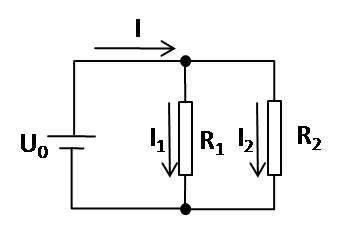
\includegraphics[width=1.00\textwidth]{Versuch_13-14/Abbildungen/Parallel.jpg}
 \label{fig:Parallel}
\end{minipage}
%
\begin{minipage}{0.6\textwidth}
Aus der Knotenregel folgt: \hfill $I = I_1 + I_2\, .$\\
Mit dem Ohm'schen Gesetz folgt: \hfill $\frac{U_0}{R_{ges}} = \frac{U_0}{R_1} + \frac{U_0}{R_2}\, .$\\
Den Gesamtwiderstand der Parallelschaltung von Widerständen kann man also schreiben als: 
\begin{equation}
\frac{1}{R_{ges}} = \frac{1}{R_1} + \frac{1}{R_2} = \sum_i{\frac{1}{R_i}} \, .
\end{equation}
\end{minipage}
%
\subsection{Serienschaltung}

\begin{minipage}{0.35\textwidth}
 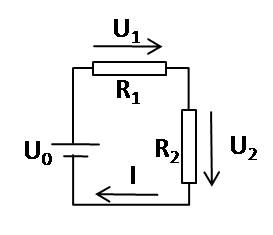
\includegraphics[width=1.00\textwidth]{Versuch_13-14/Abbildungen/Seriell.jpg}
 \label{fig:Seriell}
\end{minipage}
%
\begin{minipage}{0.6\textwidth}
Aus der Maschenregel folgt: \hfill $U_0 = U_1 + U_2\, .$\\
Mit dem Ohm'schen Gesetz folgt: \hfill $I R_{ges} = I R_1 + I R_2\, .$\\
Den Gesamtwiderstand der Serienschaltung von Widerständen kann man also schreiben als: 
\begin{equation}
R_{ges} = R_1 + R_2 = \sum_i{R_i} \, .
\end{equation}
\end{minipage}
%
\subsection{Der (unbelastete) Spannungsteiler}

In Schaltung \ref{fig:Seriell} kann man die Spannung $U_2$, die über den Widerstand $R_2$ abfällt auch als Eingangsspannung für eine daran anschliessende Schaltung benutzen. Schaltung \ref{fig:Seriell} bezeichnet man in diesem Fall als \textit{Spannungsteiler}. Die Spannung $U_2$ wird dann durch die \textit{Spannungsteilerformel} gegeben, die wir kurz herleiten wollen:\\
Fließt ein Strom $I$ durch $R_2$, so fällt über den Widerstand die Spannung ab
\begin{equation*}
U_2 = I\cdot R_2\; .
\end{equation*}
Aus der Maschenregel folgt für den Strom:
\begin{equation*}
I = \frac{U_0}{R_1 + R_2} \; .
\end{equation*}
Einsetzen ergibt die Spannungsteilerformel:
\begin{equation}
U_2 = U_0\cdot\frac{R_2}{R_1+R_2}
\end{equation}

\subsection{Die Wheatstone'sche Brückenschaltung}

Widerstände im Bereich von 0,01 $\Omega$ bis 10 M$\mathrm{\Omega}$ werden oft mit einer Meßbrückenschaltung nach Wheatstone (siehe Abbildung rechts) gemessen. Der zu messende Widerstand sei $R_3$. Er läßt sich bei \"abgeglichener\" Brücke, d.h. wenn kein Strom durch das Amperemeter fließt, aus der Beziehung
\begin{equation}
 R_3 = R_4\frac{R_1}{R_2}
 \label{eq:Wheatstone}
\end{equation}
berechnen. Durch das Amperemeter fließt nämlich nur dann kein Strom, wenn die Punkte C und D auf demselben Potenzial liegen. Es muss also gelten

\begin{minipage}[b]{0.5\textwidth}
\begin{equation}
 U_{AC} = U_{AD},
\end{equation}
woraus folgt
\begin{equation}
 R_1 I_1 = R_3 I_3.
\end{equation}
Gleichzeitig muss gelten
\begin{equation}
 U_{CB} = U_{DB},
\end{equation}
woraus folgt
\begin{equation}
 R_2 I_2 = R_4 I_4.
\end{equation}

Da bei abgeglichener Brücke $I_1 = I_2$ und $I_3 = I_4$ ist, folgt für $R_3$ Gleichung \ref{eq:Wheatstone}.
\end{minipage}
%
\begin{minipage}[b]{0.5\textwidth}
 \centering
 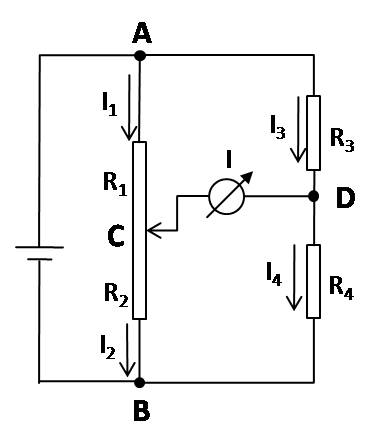
\includegraphics[width=0.7\textwidth]{Versuch_13-14/Abbildungen/Wheatstone_Prinzip.jpg}\\
 Brückenschaltung nach Wheatstone.
\end{minipage}


%------------------------------------------------
\section{Fragen zur Vorbereitung}
%------------------------------------------------

\begin{enumerate}
 %
 \item Was soll heute im Praktikum gemessen werden? Warum?
 %
 \item Wiederholung: Definition von Strom und Spannung
 %
 \item Wiederholung: Ohm'sches Gesetz, Schaltung von Messgeräten
 %
 \item Wie lauten die Kirchhoff'schen Gesetze? Welche Erhaltungssätze liegen ihnen zugrunde?
 %
 \item Wie berechnet man den Gesamtwiderstand bei Reihen- und Parallelschaltungen von Widerständen?
 %
 %\item Was ist ein Innenwiderstand?
 %
 \item Wie funktioniert die Spannungsteilerschaltung (Schaltskizze und Erklärung)?
 %
 \item Wie funktioniert die Wheatstone'sche Brückenschaltung (Schaltskizze und Erklärung)? Was kann man mit ihr messen?
\end{enumerate}

%------------------------------------------------
\section{Durchführung} 
%------------------------------------------------

\begin{minipage}{0.6\textwidth}
 \begin{enumerate}
  %
  \item Der unbekannte Widerstand $R_1$ soll mithilfe des Ohm'schen Gesetzes bestimmt werden.\\
   Erh"ohen Sie die Ausgangsspannung der regelbaren Spannungsquelle $U_1$ von 0,5\,V bis 6\,V in Schritten von 0,5\,V. Messen Sie f"ur jede Spannung den Gesamtstrom $I$ mit dem Amperemeter.\\
   Anmerkung: Ver"andern Sie w"ahrend der Messung den Widerstand $R_X$ nicht. Dann k"onnen $R_2$ und $R_x$ zum Innenwiderstand $R_i$ zusammengfasst werden, der hier nicht betrachtet werden muss.
  %
 \end{enumerate}
\end{minipage}
%
\begin{minipage}{0.35\textwidth}
 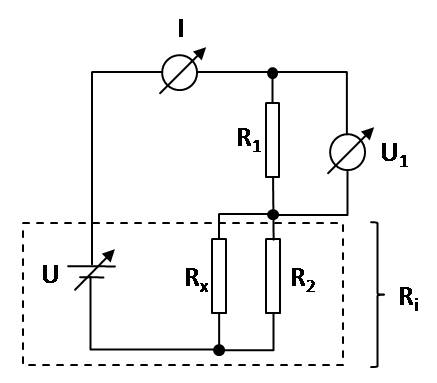
\includegraphics[width=1.00\textwidth]{Versuch_13-14/Abbildungen/Schaltung1.jpg}
 \label{fig:Schaltung1}
\end{minipage}

\begin{enumerate} \setcounter{enumi}{1}
 %
 \item Messen Sie die feste Ausgangsspannung $U_k$ mit dem Voltmeter.
 %
 \item Die drei unbekannten Widerstände $R_x$(1,2,3) sollen nach den beiden Schaltungen A und B gemessen werden. Messen Sie dazu in Schaltung A den Spannungsabfall $U_1$ am Widerstand $R_1$ und in Schaltung B den Gesamtstrom $I_1$.
 %
\end{enumerate}

%\begin{figure}[h]
\begin{minipage}[b]{0.5\textwidth}
 \centering
 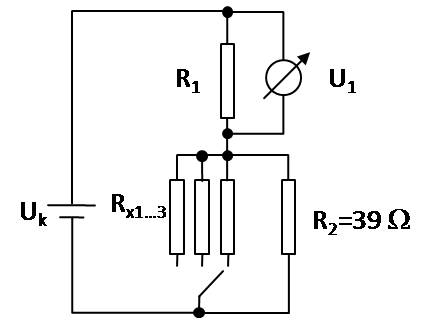
\includegraphics[width=0.7\textwidth]{Versuch_13-14/Abbildungen/SchaltungA.jpg}\\
 Schaltung A
\end{minipage}
%
\begin{minipage}[b]{0.5\textwidth}
 \centering
 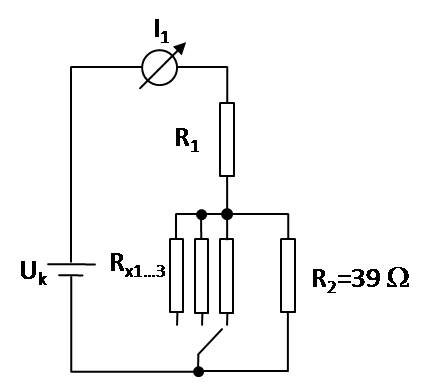
\includegraphics[width=0.7\textwidth]{Versuch_13-14/Abbildungen/SchaltungB.jpg}\\
 Schaltung B
\end{minipage}
%\end{figure}

%\begin{figure}[h]
\begin{minipage}[b]{0.6\textwidth}
\begin{enumerate} \setcounter{enumi}{3}
 %
 \item Die Innenwiderstände der Spannungsquelle und des Amperemeters sollen gemessen werden. Messen Sie dazu in Schaltung C den Gesamtstrom $I_g$ sowie die Spannung über die Lastwiderstände $U_L$. Die Größe des Widerstandes $R_3$ kann gegenüber dem großen Innenwiderstand des Voltmeters ($\approx\, 10\,M\Omega$) vernachlässigt werden. Dann berechnet sich der Innenwiderstand der Spannungsquelle nach
 \begin{equation}
  R_i = \frac{U_k - U_L}{I_g}\, .
 \end{equation}
 %
\end{enumerate}
\end{minipage}
%
\begin{minipage}[b]{0.35\textwidth}
 \centering
 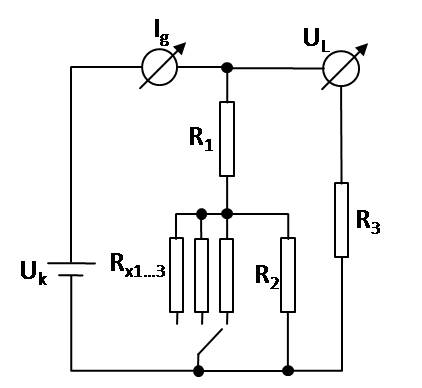
\includegraphics[width=0.8\textwidth]{Versuch_13-14/Abbildungen/SchaltungC.jpg}\\
 Schaltung C
\end{minipage}
%\end{figure}

%\begin{figure}[h]
\begin{minipage}[b]{0.6\textwidth}
\begin{enumerate} \setcounter{enumi}{4}
 %
 \item Mithilfe der Wheatstone'schen Brückenschaltung sollen die drei unbekannten Widerstände $R_y$ (y=1,2,3) bestimmt werden. \\
  Bauen sie den Versuch auf der rechten Hälfte des Experimentierschaltkreises auf. Betreiben Sie hierbei das Amperemeter im empfindlichsten Bereich.\\
  Verdrehen Sie nun das Potentiometer $R_3$ so lange, bis kein Strom mehr durch das Amperemeter fließt.\\
  Die Ablesung 'X' am Potentiometer bedeutet
  \begin{equation}
   \frac{R_{3b}}{R_{3a}} = \frac{X}{100 - X}
  \end{equation}
  und ist damit nicht direkt der Widerstand.
 %
\end{enumerate}
\end{minipage}
%
\begin{minipage}[b]{0.35\textwidth}
 \centering
 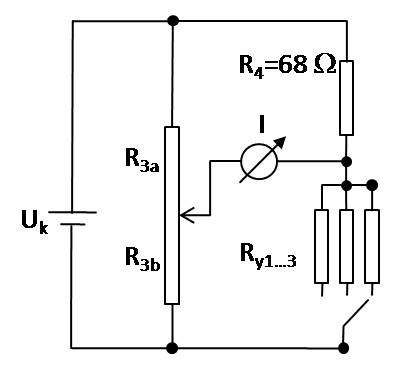
\includegraphics[width=0.8\textwidth]{Versuch_13-14/Abbildungen/Wheatstone.jpg}
 \label{fig:Wheatstone}\\
 Wheatsone'sche Brückenschaltung
\end{minipage}
%\end{figure}

%\pagebreak

%------------------------------------------------
\section{Auswertung} 
%------------------------------------------------

\begin{enumerate}
 %
 \item Berechnen Sie den Mittelwert des Widerstands $R_1$ inkl. seines Fehlers.
 %
 \item Leiten Sie die Formel für den Widerstand $R_x$ in Schaltung A her.\\
  Anleitung: Berechnen Sie den Gesamtwiderstand der Parallelschaltung von $R_x$ und $R_2$. Zusammen mit der Spannungsteilerformel erhält man schließlich:
  \begin{equation}
   R_x = R_2 \frac{1-\frac{U_k}{U_1}}{\frac{U_k}{U_1}-\frac{R_2}{R_1}-1}
  \end{equation}
 %
 \item Leiten Sie die Formel für den Widerstand $R_x$ in Schaltung B her.\\
  Anleitung: Drücken Sie $U_1$ durch den Strom $I$ aus. Danach, wie oben, einfach nach $R_x$ auflösen. Dann finden Sie:
  \begin{equation}
   R_x = R_2 \frac{R_1 - \frac{U_k}{I}}{\frac{U_k}{I}-R_1-R_2}
  \end{equation}
 %
 \item Berechnen Sie nun die Widerstände $R_x$ (x=1,2,3) aus Schaltung A und B mit ihrem Fehler. 
  Benutzen Sie eine Ungenauigkeit ($\hat{=}$ Fehler) für die Messungen der Ströme und Spannungen von 1\% .
 %
 \item Berechnen Sie den Innenwiderstand der Spannungsquelle.
 %
 \item Berechnen Sie den Widerstand $R_y$ (y=1,2,3) aus der Wheatstoneschen Brückenschaltung.\\
  Hinweis: Aus der Bedingung, dass durch das Amperemeter kein Strom fließt, ergibt sich:
  \begin{equation}
   R_y = R_4\frac{R_{3b}}{R_{3a}} \; .
  \end{equation}
\end{enumerate}	% Elektrische Netzwerke
\chapter{Nichtstationäre Diffusion}
\label{v:14}

In diesem Versuch betrachten Sie, wie ein Farbstoff in Wasser diffundiert. Dabei messen Sie die momentane Konzentration des Farbstoffes mithilfe eines lichtempfindlichen Widerstandes.

%------------------------------------------------
\section{Stichworte}
%------------------------------------------------

Wheatstone'sche Brückenschaltung; Photowiderstand; Brown'sche Molekularbewegung; stationäre und nichtstationäre Diffusion; Fick'sche Gesetze; Diffusionkoeffizient; Diffusionsgleichung.
%
%------------------------------------------------
\section{Literatur}
%------------------------------------------------

Gehrtsen, Kapitel 5.2.8 und 5.4
%
%------------------------------------------------
\section{Anwendungsbeispiele}
%------------------------------------------------

Diffusion spielt sowohl in der Natur, als auch in zahlreichen technischen Anwendungen eine tragende Rolle.\\
Zum Beispiel geschieht der Gasaustausch zwischen Lungenbläschen und Blut bei der Lungenatmung durch Diffusion, genauso wie der Transport bestimmter Stoffe durch Membranen (teilweise sog. erleichterte Diffusion). \\
Beim Sintern von Werkstoffen spielt die Diffusion eine wichtige Rolle beim Zusammenwachsen der Pulverbestandteile, in der Halbleiterindustrie wird sie benutzt, um Dotierungsstoffe in das Halbleitermaterial einzubringen. In der technischen Chemie spielt Diffusion, gekoppelt mit Konvektion und chemischen Reaktionen eine zentrale Rolle im Reaktor- und Katalysatordesign.

%------------------------------------------------
\section{Theoretischer Hintergrund}
%------------------------------------------------

\subsection{Diffusion in Gasen und Lösungen}

Schichtet man Alkohol vorsichtig über Wasser oder reines Wasser über eine Salzlösung, dann wird die anfangs scharfe Trennfläche allmählich diffuser. Die steile Dichtestufe flacht sich mit der Zeit immer mehr ab. In Lösungen dauert diese Durchmischung Stunden, in Gasen nur Sekunden.\\
Diese Diffusion findet immer dann statt, wenn die Konzentration eines gelösten Stoffes, der Druck eines Gases oder der Partialdruck eines Bestandteiles eines Gasgemisches, allgemein also wenn die Teilchenzahldichte $n$ von Ort zu Ort unterschiedlich ist. Der Vorgang endet erst, wenn die Teilchendichte an allen Punkten des zur Verfügung stehenden Volumens gleich groß ist, falls Teilchen dieses nicht verlassen oder von außen hereinkommen können. Zustande kommt diese Bewegung der Teilchen durch ihre thermische Energie (Brown'sche Bewegung).\\
Der Teilchentransport in der Diffusion wird durch den Gradienten der Teilchenzahldichte, $\mathrm{grad} n$, angetrieben. Die \textit{Teilchenstromdichte} $\vec{j}_n$, ein Vektor, dessen Betrag die Anzahl von Teilchen darstellt, die pro Sekunde durch die Flächeneinheit treten, ist proportional zum Gefälle von $n$:\\

1. Ficksches Gesetz:
\begin{equation}
 \vec{j}_n = -D\,\mathrm{grad}\, n.
 \label{eq:Fick1}
\end{equation}

Der Diffusionstrom fließt immer in die Richtung, in die $n$ am schnellsten abnimmt. $D$ ist der Diffusionskoeffizient, dessen Einheit $\left[D\right] = \mathrm{m^2/s}$ ist.\\

Wenn aus einem Volumen mehr Teilchen ausströmen als hineinfließen, nimmt die Teilchenzahl dort ab:
\begin{equation}
 \dot{n} = -\mathrm{div}\,\vec{j}_n\; .
\end{equation}

Mit Gleichung \ref{eq:Fick1}) erhält man die allgemeine Diffusionsgleichung\\

2. Ficksches Gesetz:
\begin{equation}
 \dot{n} = D\,\mathrm{div}\,\mathrm{grad}\, n = D\,\Delta n\; .
\end{equation}

Diese Art der Diffusion, die durch einen Konzentrationsgradienten getrieben wird, nennt man auch \textit{nichtstationäre Diffusion}. Ihr gegenüber steht die \textit{stationäre Diffusion}, auch Selbstdiffusion genannt, die beschreibt wie sich Teilchen innerhalb derselben Substanz bewegen. Da die Teilchen prinzipiell ununterscheidbar sind, ist die stationäre Diffusion allerdings sehr schwierig zu beobachten.
%------------------------------------------------
\section{Fragen zur Vorbereitung}
%------------------------------------------------

\begin{enumerate}
 %
 %\item Was soll heute im Praktikum gemessen werden? Warum?
 %%
 \item Was ist eine Wheatstone'sche Brückenschaltung? Wie funktioniert sie?
 %
 \item Was ist ein Photowiderstand?
 %
 \item Was versteht man unter Brown'scher Molekularbewegung? Wodurch entsteht sie?
 %
 \item Welcher Effekt wird als Diffusion bezeichnet?
 %
 %\item Was ist stationäre bzw. nichtstationäre Diffusion?
 %
 \item Was ist die Bedeutung der Diffusionskonstanten D (Diffusionsgleichung für stationäre Diffusion) ?
 %
 \item Wie wird ein Photowiderstand zusammen mit einer Wheatstone Brücke zur Messung der Diffusion benutzt ?
%
\end{enumerate}

%------------------------------------------------
\section{Durchführung} 
%------------------------------------------------

\begin{minipage}{0.6\textwidth}
 \begin{enumerate}
  %
  \item Bauen Sie zunächst die Wheatstone'sche Brückenschaltung auf.\\
  
   Der Strom, den das Amperemeter zeigt, hängt bei vorgegebenem Vergleichswiderstand $R_V$ von der Potentiometereinstellung und von dem elektrischen Widerstand des Photowiderstandes $R_P$ ab. Dieser
   Widerstand ist durch die Lichtmenge bestimmt, die auf den Photowiderstand fällt.
  %
 \end{enumerate}
\end{minipage}
%
\begin{minipage}{0.35\textwidth}
 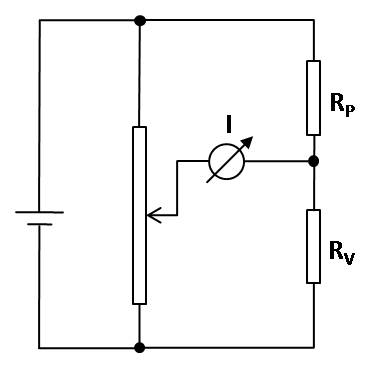
\includegraphics[width=1.00\textwidth]{Versuch_13-14/Abbildungen/Wheatstone14.jpg}
 \label{fig:Schaltung1}
\end{minipage}

\begin{enumerate} \setcounter{enumi}{1}
 %
 \item Stellen Sie den Strahlengang so ein, dass der Beleuchtungsspalt scharf auf den zweiten Spalt abgebildet wird, hinter dem sich der Photowiderstand befindet. Das Amperemeter in der Brückenschaltung zeigt dann den maximalen Strom an. Fixieren Sie den Strahlengang in dieser Konfiguration.
 %
 \item Schieben Sie den Graufilter C016 vor den Photowiderstand und gleichen Sie die Brückenschaltung ab, so dass das Amperemeter keinen Strom mehr anzeigt. Arretieren Sie das Potentiometer in dieser Stellung.
 %
 \item Füllen Sie die Diffusionsküvette zu drei Vierteln mit Wasser und bringen Sie sie anstelle des Graufilters in den Strahlengang, so dass die Wasseroberfläche sich auf gleicher Höhe mit dem Lichtstrahl befindet.
 %
 \item Geben Sie einige Tropfen Farbstofflösung der Anfangskonzentration $C_0$ auf das Wasser und starten Sie zur gleichen Zeit die Stoppuhr ($t=0$).
 %
 \item Verschieben Sie nun die Küvette mittels des Höhentriebes so weit, dass sich die Farbzone mit der Konzentration $C = 1/16\; C_0$ vor dem Spalt befindet.\\
  Diese Farbzone absorbiert Licht genauso stark wie der Graufilter, also zeigt das Amperemeter bei richtiger Einstellung wieder keinen Strom mehr an ($I = 0$). Notieren Sie den Ort $x$ der Farbzone, den man am Höhentrieb ablesen kann.
 %
 \item Wiederholen Sie diese Einstellung zu den Zeiten t = 1, 2, 4, 6, 9, 12, 16, 19, 22, 25, 27, 30, 33, 36 Minuten und notieren Sie jeweils den Ort der Farbzone.
 %
\end{enumerate}

\subsection*{Hinweise:}
\begin{itemize}
 %
 \item Halten sie während der Messung nicht die Stoppuhr an und verstellen Sie nicht das Potentiometer.
 %
 \item Verstellen Sie stets nur den Höhentrieb der Küvette. Bei Manipulation im Strahlengang stellen Sie das Amperemeter auf den Messbereich 'grob'.
 %
 \item Vermeiden Sie größere Erschütterungen des Tisches.
 %
 \item Reinigen und trocknen Sie bitte nach Ende des Versuchs die Küvette gründlich.
 %
\end{itemize}

%------------------------------------------------
\section{Auswertung} 
%------------------------------------------------

\begin{enumerate}
 %
 \item Tragen Sie den Ort $x$ als Funktion von $\sqrt{t}$ graphisch auf. \label{Aufg:1}
 %
 \item Berechnen Sie aus der Steigung der Geraden den Diffusionskoeffizienten $D$ nach:
  \begin{equation}
   D = \frac{x^2}{t}\cdot f\left(\frac{C}{C_0}\right)
  \end{equation}
	
	\noindent
	Bemerkung:\\ 
	\noindent
	$f\left(C/C_0\right) = f\left(1/16\right) = 0,212$ ist ein numerischer Faktor, der die Abhängigkeit des Diffusionskoeffizienten $D$ von der Konzentration der beobachteten Farbzone angibt.
 %
 \item Schätzen Sie den Fehler von $D$ aus den Grenzgeraden der Auftragung aus Aufgabe \ref{Aufg:1}) ab.
 %
\end{enumerate} 	% Nichtstation�re Diffusion

\documentclass[11pt, twoside, a4paper]{book}

\usepackage{graphicx}
\usepackage[utf8]{inputenc}
\usepackage{ngerman}
%\usepackage{lineno}
\usepackage{verbatim}
\usepackage[squaren]{SIunits}
\usepackage{amsmath}
\usepackage{amsfonts}
\usepackage{amssymb}
\usepackage{enumitem}
\usepackage{fancyhdr}
\usepackage{textcomp}
\usepackage{subcaption}
\usepackage[noadjust]{marginnote}
\usepackage{tikz}
\usepackage{nicefrac}
\usepackage{framed}
\usepackage{import}

\usetikzlibrary{calc,intersections}
\usetikzlibrary{arrows}
\usetikzlibrary{decorations.markings}
\usetikzlibrary{decorations.pathreplacing}
\usepackage[european resistors]{circuitikz}
\usepackage[ 
    top=2cm, 
    bottom=2cm, 
    outer=3cm, 
    inner=3cm,
    marginparwidth=2.5cm,
		headheight=14pt
  ]{geometry}

\usepackage{parskip}
\usepackage{pdfpages}

 \newcommand{\Ohm}{$\mathrm\Omega$}

\setlength{\parindent}{0pt}

\newcommand{\experimentheader}[4]
{
  \iftutor{{\bf Schwierigkeitsgrad:} #1\\}
  \iftutor{{\bf Dauer:} #2\\}
  {\bf Ger\"ate:} #3\\
  {\bf Bauteile:} #4
}

\newcommand{\hintboxNone}{0}
\newcommand{\hintboxExclamation}{1}
\newenvironment{hintbox}[4][\hsize]
{
  \def\FrameCommand
  {%
    {\color{#3}\vrule width 3pt}%
    \hspace{0pt}%must no space.
    \fboxsep=\FrameSep\colorbox{#4}%
  }%
  \MakeFramed{\hsize#1\advance\hsize-\width\FrameRestore}%
  \mbox{\textbf{#2}:}%
}
{
  \endMakeFramed
}
\newcommand{\xhintbox}[3]
{
  \begin{hintbox}{Achtung}{red!50}{red!10}
    #3
  \end{hintbox}
}

\newenvironment{hint}
{
  \begin{hintbox}{Hinweis}{green!50}{green!10}
}
{
  \end{hintbox}
}

\newenvironment{definition}
{
  \begin{hintbox}{Definition\\}{white!50}{white!10}
}
{
  \end{hintbox}
}

\newenvironment{important}
{
  \begin{hintbox}{Hinweis}{gray!50}{gray!10}
}
{
  \end{hintbox}
}

\newenvironment{jason}
{
  \begin{hintbox}{Achtung}{red!50}{red!10}
}
{
  \end{hintbox}
}

\newcommand{\mandatoryenumi}
{
  \renewcommand{\labelenumi}{\arabic{enumi}.} 
}
\newcommand{\optionalenumi}
{
  \renewcommand{\labelenumi}{$\bigstar$\quad\arabic{enumi}.} 
}
\newcommand{\mandatoryenumii}
{
  \renewcommand{\labelenumii}{(\alph{enumii})} 
}
\newcommand{\optionalenumii}
{
  \renewcommand{\labelenumii}{$\bigstar$\quad(\alph{enumii})} 
}
\newcommand{\icname}[1]{\mbox{\tt #1}}


  %\newcommand{\iftutor}[1]{}
\newcommand{\ifnotutor}[1]{#1}

  \newcommand{\iftutor}[1]{#1}
\newcommand{\ifnotutor}[1]{}


\newenvironment{tutorhint}{\comment}{\endcomment}
\newenvironment{todo}{\comment}{\endcomment}
\newenvironment{solution}{\comment}{\endcomment}
\iftutor
{
  \renewenvironment{todo}
  {
    \hintbox{Todo}{red!50!yellow!90}{red!50!yellow!20}
  }
  {
    \endhintbox
  }
  \renewenvironment{tutorhint}
  {
    \hintbox{Tutorenhinweis der Stunde}{blue!50}{blue!10}
  }
  {
    \endhintbox
  }
  \renewenvironment{solution}
  {
    \hintbox{L\"osung}{black!80}{black!5}
  }
  {
    \endhintbox
  }
}
\newcommand{\etutorhint}[1]
{
  \iftutor{
    \tutorhint
      #1
    \endtutorhint
  }
}
\newcommand{\esolution}[1]
{
  \iftutor
  {
    \solution
    #1
    \endsolution
  }
}
\newcommand{\etodo}[1]
{
  \iftutor
  {
    \todo
    #1
    \endtodo
  }
}



\begin{document}

\renewcommand{\thechapter}{\arabic{chapter}}
\setcounter{chapter}{18}
\def\chaptername{Versuch}

\chapter{Künstliche Radioaktivität}
\label{v:19}

In diesem Versuch studieren Sie die Grundlagen radioaktiver Zerfälle, wie z. Bsp. das zeitliche Abklingverhalten.

%------------------------------------------------
\section{Stichworte}
%------------------------------------------------

Radioaktiver Zerfall; Geiger-Müller-Zählrohr; Aufbau der Atomkerne; Zerfallsgesetz; Aktivität; Lebensdauer; Halbwertzeit; natürliche Radioaktivität; $\alpha-,\,\beta-,\,\gamma-$Zerfall.
%
%------------------------------------------------
\section{Literatur}
%------------------------------------------------

Gehrtsen, Kapitel 13.1 und 13.2.1-3
%
%------------------------------------------------
\section{Sicherheitshinweise}
%------------------------------------------------

\begin{minipage}{0.4\textwidth}
	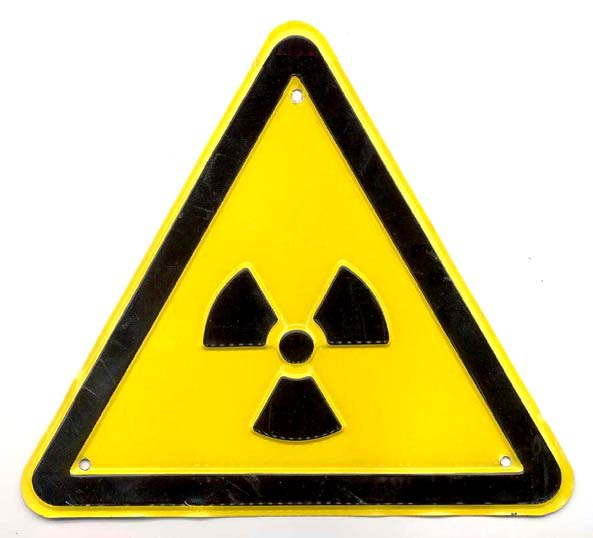
\includegraphics[width=\textwidth]{Abbildungen/Schild.jpg}
	\label{fig:Schild}
\end{minipage}
%
\begin{minipage}{0.6\textwidth}
	\begin{itemize}
		%
		\item Gekennzeichnete Kontroll- oder Sperrbereiche dürfen nicht betreten werden.
		%
		\item Abstand zu einer radioaktiven Quelle halten.
		%
		\item Absorber zwischen sich und die Quelle bringen.
		%
		\item Die Neutronen-Aktivierung führt nur der Assistent durch!
		%
		\item Man halte sich nur kurzzeitig im gleichen Raum mit der Neutronenquelle auf.
		%
		\item \textbf{Schwangere und stillende Frauen dürfen diesen Versuch nicht durchführen!}
		%
	\end{itemize}
\end{minipage}

%------------------------------------------------
\section{Anwendungsbeispiele}
%------------------------------------------------

Radioaktivität und Kernreaktionen sind Bestandteile unserer natürlichen und technologischen Umwelt. Der Umgang mit diesen Prozessen ist in letzter Zeit sehr hinterfragt worden. So sind die früher üblichen grünen Leuchtziffern der Uhren, die radioaktives Radiumsalz enthielten, nicht mehr im Gebrauch. Auch die Kernenergie wird kontrovers diskutiert, obgleich sie eine viel geringere Gefahr für die Einzelperson darstellt, als z.B. der Autoverkehr. Die Gründe dafür liegen sicher unter anderem auch an der Unanschaulichkeit der Prozesse.\\
Der Versuch ''Künstliche Radioaktivität'' führt unter Beachtung der Sicherheitsaspekte in die Physik dieser Prozesse ein. Er zeigt, dass Alphateilchen Heliumkerne, dass Betastrahlen Elektronen, dass Gammastrahlen Photonen und dass Neutronen Kernbausteine sind, die in schweren Elementen mehr als die Hälfte der Masse des Atoms ausmachen. Der Beta-Zerfall ist undenkbar ohne Neutrinos, die auch 70 Jahre nach ihrer Entdeckung nichts von ihrer Faszination verloren haben.\\

\noindent
Radioaktivität spielt neben den oben genannten alltäglichen Aspekten auch als Werkzeug in den verschiedensten Gebieten der Wissenschaft eine gewichtige Rolle. Einige Beispiele sind:\\
$^{14}$C-Altersbestimmung für Archäologen, Altersbestimmung von Erde und Mond für Geologen und Planetologen, Strahlentherapie und Diagnostik in der Medizin, radioaktive Indikatoren in Chemie und Biologie, Kernreaktoren für Forschung und Energiegewinnung.

%------------------------------------------------
\section{Theoretischer Hintergrund}
%------------------------------------------------

\subsection{Radioaktive Zerfälle}

Im März des Jahres 1896 entdeckte der französische Physiker Henri Becquerel mehr oder weniger zufällig die spontane Kernumwandlung. Auf einer dichtverpackten Photoplatte, die er zur Untersuchung der Phosphoreszenz von Uransalzen verwenden wollte, hatte er ein Stück Pechblende (Uraninit, ein kristallines Oxid des Urans) liegen lassen. Bei der Entwicklung der Photoplatte fand er ein exaktes Abbild des Stückchens, was ein starker Hinweis darauf war, dass Uran eine durchdringende Strahlung aussendet. 1903 teilte sich Becquerel den Nobelpreis für Physik mit den französischen Physikern Pierre Curie und Marie Curie für ihre Arbeit zur Radioaktivität.\\

\noindent
Der Kern jedes Atoms ist aus Protonen ($p$) und Neutronen ($n$) zusammengesetzt. Um einen Kern eindeutig identifizieren zu können gibt man (nicht nur) in der Kernphysik die Kernladungszahl $Z$ (Anzahl der Protonen im Kern) und die Kernmassenzahl $A$ (Anzahl von Protonen und Neutronen) an. Ein Kern kann also dargestellt werden durch ein paar von Zahlen der Form $(A,Z)$. Allgemein bekannter ist die folgende Schreibweise:
\begin{equation*}
^A_Z X
\end{equation*}
wobei $X$ für das aus dem Periodensystem bekannten Symbol des Elementes steht. Bsp.: $^{12}_6 C$

\noindent
In späteren Untersuchungen an verschiedenen radioaktiven Isotopen wurden drei verschiedene Arten von Strahlung identifiziert, die beim Zerfall von Atomkernen entstehen können. Dies sind 
\begin{itemize}
	%
	\item \textbf{$\alpha$-Strahlung:} \\
		Heliumkerne, die überwiegend beim Zerfall sehr schwerer instabiler Kerne abgestrahlt werden. Reaktionsgleichung: $(A,Z) \rightarrow (A-4, Z-2) + ^4_2\mathrm{He}$.
	%
	\item \textbf{$\beta$-Strahlung:} Elektronen; werden beim Zerfall von Neutronen in Protonen (Halbwertszeit $T_{1/2} = 900$\,s) abgestrahlt. Reaktionsgleichung: $(A,Z) \rightarrow (A, Z+1) + e^-$.
	%
	\item \textbf{$\gamma$-Strahlung:} Photonen, hochenergetisches Licht, prinzipiell dasselbe wie Röntgenstrahlung. Reaktionsgleichung: $(A,Z) \rightarrow (A,Z) + \gamma$.
	%
\end{itemize}
Ähnlich dem Periodensystem der Elemente sind stabile und instabile Isotope aller Elemente in der \textit{Nuklidkarte} gesammelt, welche außerdem die Zerfallsart der instabiilen Isotope sowie mindestens die Halbwertszeit des Isotops angibt.\\

\subsection{Zerfallsgesetz}

Der Zerfall eines instabilen Atomkerns ist ein quantenmechanischer Prozess, weshalb es physikalisch unmöglich ist, genau vorherzusagen, nach welcher Zeit ein bestimmter Kern zerfällt. Die einzige mögliche Angabe ist die Wahrscheinlichkeit, mit der der Kern nach einer bestimmten Zeit $t$ zerfallen ist (\textit{Zerfallswahrscheinlichkeit $\lambda$}). Betrachtet man nicht nur einen einzelnen Kern, sondern ein Ensemble von Kernen, so kann man diese Zerfallswahrscheinlichkeit durch die \textit{Halbwertzeit $T_{1/2}$} ausdrücken ($\lambda = \ln(2)/T_{1/2}$). Diese gibt an, nach welcher Zeit die Hälfte der ursprünglich vorhandenen Kerne zerfallen ist.\\
Die Anzahl der Kerne, die nach einer Zeit $t$ noch nicht zerfallen sind, erhält man aus dem \textit{Zerfallsgesetz}:
\begin{equation} \label{eq:Zerfallsgesetz}
	N(t) = N_0\cdot \exp(-\lambda\, t)
\end{equation}
Dabei gibt $N_0$ die Zeit der zur Zeit $t=0$ vorhandenen Kerne an.\\

\noindent
Die \textit{Aktivität} einer radioaktiven Probe gibt die Anzahl der Zerfälle pro Zeit an. Früher wurde die Aktivität in der Einheit \textit{Curie} angegeben, wobei $1\,Ci = 3,7\cdot 10^{10}$ Zerfälle/s entspricht. Heute verwendet man die SI-Einheit \textit{Becquerel}: $1 Bq$ = 1 Zerfall/s.\\
Man erhält die Aktivität als Zeitableitung des Zerfallsgesetzes:
\begin{equation} \label{eq:Aktivitaet}
	A(t) := \left|\frac{dN(t)}{dt}\right| = A_0\cdot\exp(-\lambda\, t) = \lambda\, N(t)
\end{equation}
Wie man sieht, nimmt die Aktivität einer radioaktiven Probe exponentiell mit der Zeit ab, die Zeitkonstante is $1/\lambda$. Diese natürliche Abnahme der Aktivität nennt man Abklingen.


%------------------------------------------------
\section{Fragen zur Vorbereitung}
%------------------------------------------------

\begin{enumerate}
	%
%	\item Was soll heute im Praktikum gemessen werden? Warum?
	%
	\item Wie ist ein Atom aufgebaut?
	%
	\item Woraus besteht der Atomkern?
	%
	\item Was ist radioaktiver Zerfall?
	%
	\item Welche Zerfallsarten gibt es? (einschl. der jeweiligen Zerfallsgleichungen)
	%
	\item Wieso ist ionisierende Strahlung gefährlich, und wie kann man sich schützen?
	%
	\item Mit welchen Geräten misst man die Radioaktivität?
	%
	\item Wie funktioniert ein Geiger-Müller-Zählrohr?
	%
	\item Was ist das Zerfallsgesetz? (Herleitung !!)
	%
	\item Was versteht man unter Halbwertszeit? \\
		Wie berechnet sie sich aus der Zerfallskonstanten $\lambda$?
	%
	\item Was ist die Aktivität? Wie ist sie definiert?
	%
	\item Wieso mißt man auch ohne ein radioaktives Präparat eine von Null verschiedene Aktivität (Nulleffekt)? Woher kommt sie?
	%
\end{enumerate}

%------------------------------------------------
\section{Durchführung} 
%------------------------------------------------

\begin{enumerate}
	%
	\item Messen Sie die Untergrundzählrate über 10 Minuten mit der nicht aktivierten Silberfolie. Berechnen Sie die Anzahl der erwarteten Untergrundereignisse in 30 Sekunden.
	%
	\item Die Silberfolie wird 5 Minuten lang vom Assistenten mit Neutronen der Am-Be-Quelle aktiviert. Danach wird der zeitliche Abfall der Zählrate etwa 15 Minuten lang gemessen.\\
	Die erste Messung beginnt 30 Sekunden nach Beendigung der Aktivierung, die Zählrate wird 30 Sekunden lang gemessen, dann 10 Sekunden Pause, usw.; eine Messtabelle ist vorzubereiten !
	%
\end{enumerate}

\begin{hint}
Die Kernreaktionen, die zu kurzlebigen Silberisotopen führen, laufen wie folgt ab:
\begin{itemize}
	%
	\item In der Am-Be-Quelle entstehen $\alpha$-Teilchen beim Zerfall von Americium. Diese Teilchen fusionieren mit Beryllium-Kernen zu Kohlenstoff. Dabei tritt $\gamma$-Strahlung auf und ein Neutron wird emittiert:
		\begin{align*}
			^{241}_{95}Am \rightarrow ^{237}_{93}Np & + \alpha &\\
			^9_4 Be & + \alpha \rightarrow ^{12}_6C + n + \gamma
		\end{align*}
	%
	\item Das Neutron wird von einem der beiden natürlich vorkommenden Silber-Isotope eingefangen. Es entstehen zwei andere instabile Silber-Isotope, die verschieden kurze Lebensdauern besitzen: Die Silberfolie ist aktiviert worden.
		\begin{align*}
			^{107}_{47}Ag + n \rightarrow ^{108}_{47}Ag & \rightarrow ^{108}_{48}Cd + e^- + \bar{\nu}_e + \gamma \; . &\\
			^{109}_{47}Ag + n \rightarrow ^{110}_{47}Ag & \rightarrow ^{110}_{48}Cd + e^- + \bar{\nu}_e + \gamma \; .
		\end{align*}
	%
	\item Beide radioaktiven Silberisotope zerfallen durch $\beta$-Zerfall zu stabilen Cadmium-Isotopen. Die $\beta$-Strahlung ($e^-$) wird im Zählrohr registriert.
	%
\end{itemize}
\end{hint}

%------------------------------------------------
\section{Auswertung} 
%------------------------------------------------
\etodo{Musterauswertung}
\begin{figure}[h]
	\centering
		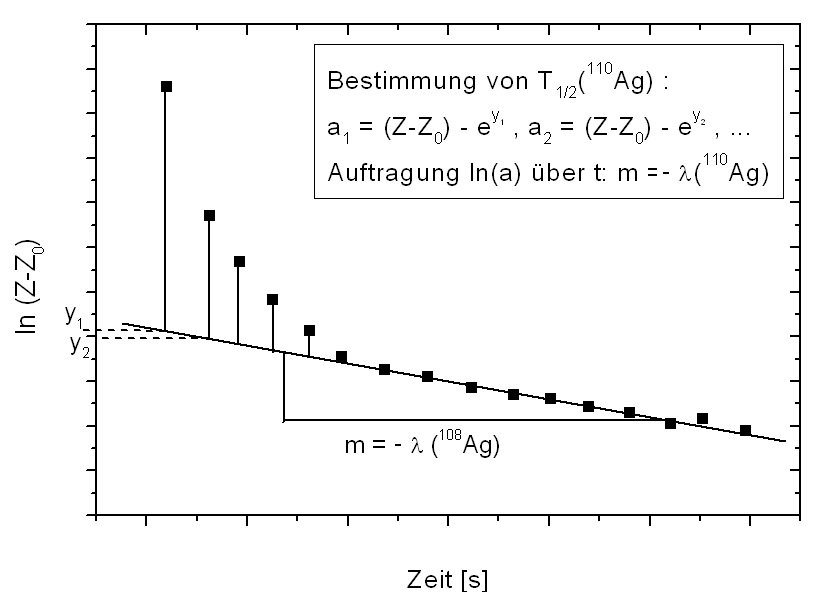
\includegraphics[width=0.5\textwidth]{Abbildungen/Bestimmung_Halbwertszeiten.jpg}
	\label{fig:Bestimmung_Halbwertszeiten}
\end{figure}

\begin{enumerate}
	%
	\item Tragen Sie, nach Abzug der Untergrundereignisse $Z_0$, die Zählrate $Z(t)$ halblogarithmisch gegen die Zeit auf, d.h. erstellen Sie einen Graphen $\ln(Z_{korr}(t))$ als Funktion der Zeit $t$, mit $Z_{korr}(t) = Z(t) -Z_0$.
	%
	\item Da es sich bei der hier ermittelten Zerfallskurve eigentlich um zwei Kernzerfälle ($^{108}Ag$ und $^{110}Ag$) handelt, ergibt die halblogarithmische Darstellung der Zählrate über der Zeit keine Gerade. Hierin macht sich der Zerfall des kurzlebigen $^{110}Ag$ bemerkbar.\\
		Bestimmen Sie zunächst aus der Auftragung die Steigung bei großen Zeiten $t$. Daraus ergibt sich die Halbwertszeit des langlebigen $^{108}Ag$.
	%
	\item Um auch die Halbwertszeit des kurzlebigen Silberisotops $^{110}Ag$ zu bestimmen, wird die Ausgleichsgerade aus Aufgabe 2) zu kurzen Zeiten hin verlängert. Dann werden die y-Werte der Ausgleichsgeraden zu den jeweiligen Zeitpunkten der Messung abgelesen ($y_1$, $y_2$, ...).\\
	Mit Hilfe dieser Werte kann von der korrigierten Zählrate $Z_{korr}$ der Anteil abgezogen werden, der durch den Zerfall des $^{108}Ag$ zustande kommt. Man berechnet also: $Z_{110} = Z_{korr} - e^y$.\\
	$Z_{110}$ soll dann halblogarithmisch für kleine Zeiten $t$ in einem neuen Graphen dargestellt werden. Hieraus kann nun die Halbwertszeit des kurzlebigen $^{110}Ag$ bestimmt werden.
	%
	\item Schätzen Sie die Fehler auf die beiden Halbwertzeiten ab und vergleichen Sie Ihre Ergebnisse mit Literaturwerten.
	%
\end{enumerate}

\end{document}	% K�nstliche Radioaktivit�t
\chapter{Spezifische Elektronenladung e/m}
\label{v:20}

In diesem Versuch wird die historische Messung der spezifischen Elektronenladung (fast originalgetreu) nachvollzogen. Dabei lernen Sie Techniken moderner Teilchenbeschleuniger und Massenspektrometern kennen.

%%%--------Bemerkung-------------------
%Eine der ersten Messungen der spezifischen Elektronenladung gelang Johann Emil Wiechert , der das Elektron etwa zeitgleich mit Joseph John Thompson entdeckte, der dafür den Nobelpreis erhielt. Wiechert arbeitete ab 1897 an der Universität Göttingen und erhielt hier 1898 den Ruf auf die weltweit erste Professur für Geophysik.

%------------------------------------------------
\section{Stichworte}
%------------------------------------------------

Erzeugung eines homogenen Magnetfeldes; Lorentzkraft; Bewegung geladener Teilchen in elektrischen und magnetischen Feldern.
%
%------------------------------------------------
\section{Literatur}
%------------------------------------------------

Gehrtsen, Kapitel 7.1.2/3 und 8.2.1/2
%
%------------------------------------------------
\section{Anwendungsbeispiele}
%------------------------------------------------

Die Messung der spezifischen Elektronenladung, die J.J. Thomson zuerst in 1897 durchführte, ist einer der größten Meilensteine in der Entdeckung der elemtaren Bausteine der Materie. Die Idee, daß Atome nicht unteilbar sind, sondern vielmehr aus grundlegenderen, sogenannten fundamentalen, Bausteinen aufgebaut seien, existierte schon vor Thomsons Messungen. Allerdings war die Annahme, daß diese Bausteine dieselbe Größe hätten, wie das kleineste bekannte Atome, das Wasserstoffatome. Basierend auf seiner Beobachtung, daß Kathodenstrahlen eine sehr viel größere Reichweite in Luft haben, als für ein Teilchen von der Größe eines Atoms zu erwarten war, schlug Thomson die Existenz eines fundamentalen Teilchens vor, welches mehr als tausendmal kleiner sei als ein Wasserstoffatom.\\
In seinem Experiment zur Messung der spezifischen Ladung der Teilchen, die die Kathodenstrahlen ausmachten fand er, daß diese sogar etwa 2000 mal größer ist, als die für ein H-Atom erwartete. Nach der Messung der Ladung dieser Teilchen im Millikan Versuch war klar, daß diese Teilchen zwar dieselbe Ladung (bis auf das Vorzeichen) wie ein H-Atomkern haben, aber etwa 2000 mal leichter sind, was die große Reichweite in Luft erklärte. Weiterhin konnte Thomson zeigen, daß Kathodenstrahlen immer aus eben diesen Teilchen bestehen, unabhängig vom Material der Kathode von der sie ausgestrahlt werden.\\
Diese Ergebnisse, die seit langem zu unserem Schulbuchwissen gehören, brachten Thomson den Nobelpreis in 1906 ein und machten ihn allgemein bekannt als den Entdecker des Elektrons.\\

\noindent
Die von Thomson benutze Technik, geladene Teilchen in elektrischen Feldern zu beschleunigen und in magnetischen Felder abzulenken, wird heute nicht nur in modernen Teilchenbeschelunigern in der Grundlagenphysik, der medizinischen Hadronen- und Strahlentherapie und der Materialprüfung eingesetzt, sondern wird auch in Massenspektrometern benutzt, um chemische Verbindungen zu charakterisieren. Beispiele hierfür sind die Identifizierung von Substanzen in Körperflüssigkeiten in der medizinischen Chemie, kriminaltechnische Untersuchungen, Dopingkontrolle und die militärische Analytik von chemischen Kampfstoffen.

%------------------------------------------------
\section{Theoretischer Hintergrund}
%------------------------------------------------

\subsection{Bewegung geladener Teilchen in E- und B-Feldern}

Geladene Teilchen werden von elektrischen und magnetischen Feldern unvergleichlich viel stärker beeinflußt als vom Gravitationsfeld (außer in der Nähe schwarzer Löcher). 

\subsubsection*{Geladene Teilchen im homogenen elektrischen Feld}

Zwischen zwei planparallelen Platten mit dem Abstand $D$ im Vakuum liegen die Spannung $U$. Wenn keine Ladungsträger zwischen den Platten das Feld verzerren, ist dieses homogen und hat die Form $\vec{E}=\frac{U}{d}\vec{e}_E$. Dieses Feld übt auf eine elektrische Ladung $Q$, welche wir in Einheiten der Ladung des Elektrons (Elemantarladung) angeben als $Q = q\cdot e$, eine Kraft $\vec{F} = qe\vec{E}$ aus und beschleunigt sie mit
\begin{equation}
	\vec{a} = \frac{qe}{m}\frac{U}{d}\vec{e}_E\; .
\end{equation}
Wie man sieht, wirkt die Kraft immer in Richtung des elektrischen Feldes. Elektrische Felder können also sowohl zur Umlenkung geladener Teilchen benutzt werden, als auch zur Beschleunigung (i.e. Erhöhung der kinetischen Energie).

\subsubsection*{Geladene Teilchen im homogenen Magnetfeld}

Wenn eine Ladung $Q = q\cdot e$ mit der Geschwindigkeit $\vec{v}$ durch ein Magnetfeld $\vec{B}$ fliegt, so erfährt sie eine Kraft 
\begin{equation}
	\vec{F} = qe\, \vec{v}\times\vec{B}\, ,
\end{equation}
die Lorentz-Karft. Diese steht, wie man am Kreuzprodukt sieht (Rechte-Hand-Regel), senkrecht auf der Bewegungsrichtung und der magnetischen Feldrichtung. Magnetfelder können damit nur zur Umlenkung geladener Teilchen benutzt werden, nicht jedoch zur Erhöhung der kinetischen Energie des Teilchens.

%------------------------------------------------
\section{Versuchsaufbau}
%------------------------------------------------

\begin{circuitikz} 
%*** power supply Box ****	
\draw[thick] (0,3) to [short, o-] (2,3)
						to [pR, n=POT] (2,0)
						to [short, -o] (0,0);
\draw[thick] (POT.wiper) to [short, -o, l=''Heizung''] (4,1.5);
\draw[thick] (2,0) to [short, *-o, l=''Kathode''] (4,0);

%*** Kabel ***
\draw [thick, dashed] (4,1.5) to [out=45, in=135] (6,1.5);
\draw [thick, dashed] (4,0) to [out=45, in=135] (6,0);

%*** Vakuumr�hre ***
\draw[thick] (6,1.5) to [short, o-] (7,1.5)
						to [L] (7,0)
						to [short, -o] (6,0);
\end{circuitikz}

%------------------------------------------------
\section{Fragen zur Vorbereitung}
%------------------------------------------------

\begin{enumerate}
	%
	\item Was soll heute im Praktikum gemessen werden? Warum?
	%
	\item Wie lautet der Ausdruck für die Kraft zwischen zwei Punktladungen?
	%
	\item Wie berechnet sich das elektrische Feld eines Plattenkondensators aus der Spannung $U$ und dem Plattenabstand $d$?
	%
	\item Welche Geschwindigkeit hat ein Teilchen, wenn es eine Spannung $U$ durchläuft?
	%
	\item Was ist die Lorentz-Kraft? Wie ist sie definiert?
	%
	\item Wie sieht die Bahnkurve eines geladenen Teilchens aus, wenn es sich senkrecht zu einem Magnetfeld bewegt?
	%
	\item Was ist ein homogenes Magnetfeld?
	%
	\item Wie lautet der Ausdruck für die Zentrifugalkraft?
	%
	\item Wie berechnet sich aus Zentrifugalkraft und Lorentzkraft ein Ausdruck für die Spezifische Elektronenladung $e/m$?
	%
\end{enumerate}

%------------------------------------------------
\section{Durchführung} 
%------------------------------------------------

Ein Elektronenstrahl beschreibt im Magnetfeld $B$ zweier Helmholtzspulen eine Kreisbahn. Die Spulen werden wie in der Abbildung unten verschaltet.

\begin{figure}[h]
	\centering
		\includegraphics[width=0.50\textwidth]{Versuch_19-20/Abbildungen/Schaltung-HHSpulen.jpg}
	\label{fig:Schaltung-HHSpulen}
\end{figure}

\textbf{Hinweis:} Lassen Sie Ihre Schaltung vor dem Einschalten durch den Betreuer überprüfen. Schalten Sie die Anodenspannung erst ein, wenn der Kathodenzylinder rot glüht.\\

\noindent
Messen Sie für verschiedene Anodenspannungen: $U$ = (125, 150, ..., 225\,V) und Spulenstromstärken: $I$ = (0.6, 0.7, ..., 0.9\,A) den maximalen Durchmesser $d$ dieser Kreisbahn. Berechnen Sie für einen Messpunkt $e/m$ nach untenstehender Formel.

%------------------------------------------------
\section{Auswertung} 
%------------------------------------------------

\begin{enumerate}
	%
	\item Leiten Sie die Gleichung her:
		\begin{equation}
			\frac{U}{B^2} = \frac{er^2}{2m}
		\end{equation}
		Nehmen Sie das Magnetfeld $B$ dabei als konstant an.
	%
	\item Tragen Sie $U/B^2$ als Funktion von $r^2/2$ graphisch auf. Berechnen Sie aus der Steigung der Geraden durch die Messpunkte die spezifische Elektronenladung $e/m$ inklusive Fehler.
\end{enumerate}

\textbf{Hinweis:} Zwischen dem Magnetfeld $B$ und dem Spulenstrom $I$ besteht ein linearer Zusammenhang. Die graphische Darstellung der Funktion $B$ = f($I$) für das benutzte Spulenpaar befindet sich auf der nächsten Seite !!

\begin{figure}[h]
	\centering
		\includegraphics[width=1.00\textwidth]{Versuch_19-20/Abbildungen/Eichung-HHSpulen.jpg}
	\label{fig:Eichung-HHSpulen}
\end{figure}
	% Spezifische Elektronenladung e/m

\documentclass[11pt, twoside, a4paper]{book}

\usepackage{graphicx}
\usepackage[utf8]{inputenc}
\usepackage{ngerman}
%\usepackage{lineno}
\usepackage{verbatim}
\usepackage[squaren]{SIunits}
\usepackage{amsmath}
\usepackage{amsfonts}
\usepackage{amssymb}
\usepackage{enumitem}
\usepackage{fancyhdr}
\usepackage{textcomp}
\usepackage{subcaption}
\usepackage[noadjust]{marginnote}
\usepackage{tikz}
\usepackage{nicefrac}
\usepackage{framed}
\usepackage{import}

\usetikzlibrary{calc,intersections}
\usetikzlibrary{arrows}
\usetikzlibrary{decorations.markings}
\usetikzlibrary{decorations.pathreplacing}
\usepackage[european resistors]{circuitikz}
\usepackage[ 
    top=2cm, 
    bottom=2cm, 
    outer=3cm, 
    inner=3cm,
    marginparwidth=2.5cm,
		headheight=14pt
  ]{geometry}

\usepackage{parskip}
\usepackage{pdfpages}

\setlength{\parindent}{0pt}

\newcommand{\experimentheader}[4]
{
  \iftutor{{\bf Schwierigkeitsgrad:} #1\\}
  \iftutor{{\bf Dauer:} #2\\}
  {\bf Ger\"ate:} #3\\
  {\bf Bauteile:} #4
}

\newcommand{\hintboxNone}{0}
\newcommand{\hintboxExclamation}{1}
\newenvironment{hintbox}[4][\hsize]
{
  \def\FrameCommand
  {%
    {\color{#3}\vrule width 3pt}%
    \hspace{0pt}%must no space.
    \fboxsep=\FrameSep\colorbox{#4}%
  }%
  \MakeFramed{\hsize#1\advance\hsize-\width\FrameRestore}%
  \mbox{\textbf{#2}:}%
}
{
  \endMakeFramed
}
\newcommand{\xhintbox}[3]
{
  \begin{hintbox}{Achtung}{red!50}{red!10}
    #3
  \end{hintbox}
}

\newenvironment{hint}
{
  \begin{hintbox}{Hinweis}{green!50}{green!10}
}
{
  \end{hintbox}
}

\newenvironment{definition}
{
  \begin{hintbox}{Definition\\}{white!50}{white!10}
}
{
  \end{hintbox}
}

\newenvironment{important}
{
  \begin{hintbox}{Hinweis}{gray!50}{gray!10}
}
{
  \end{hintbox}
}

\newenvironment{jason}
{
  \begin{hintbox}{Achtung}{red!50}{red!10}
}
{
  \end{hintbox}
}

\newcommand{\mandatoryenumi}
{
  \renewcommand{\labelenumi}{\arabic{enumi}.} 
}
\newcommand{\optionalenumi}
{
  \renewcommand{\labelenumi}{$\bigstar$\quad\arabic{enumi}.} 
}
\newcommand{\mandatoryenumii}
{
  \renewcommand{\labelenumii}{(\alph{enumii})} 
}
\newcommand{\optionalenumii}
{
  \renewcommand{\labelenumii}{$\bigstar$\quad(\alph{enumii})} 
}
\newcommand{\icname}[1]{\mbox{\tt #1}}


  %\newcommand{\iftutor}[1]{}
\newcommand{\ifnotutor}[1]{#1}

  \newcommand{\iftutor}[1]{#1}
\newcommand{\ifnotutor}[1]{}


\newenvironment{tutorhint}{\comment}{\endcomment}
\newenvironment{todo}{\comment}{\endcomment}
\newenvironment{solution}{\comment}{\endcomment}
\iftutor
{
  \renewenvironment{todo}
  {
    \hintbox{Todo}{red!50!yellow!90}{red!50!yellow!20}
  }
  {
    \endhintbox
  }
  \renewenvironment{tutorhint}
  {
    \hintbox{Tutorenhinweis der Stunde}{blue!50}{blue!10}
  }
  {
    \endhintbox
  }
  \renewenvironment{solution}
  {
    \hintbox{L\"osung}{black!80}{black!5}
  }
  {
    \endhintbox
  }
}
\newcommand{\etutorhint}[1]
{
  \iftutor{
    \tutorhint
      #1
    \endtutorhint
  }
}
\newcommand{\esolution}[1]
{
  \iftutor
  {
    \solution
    #1
    \endsolution
  }
}
\newcommand{\etodo}[1]
{
  \iftutor
  {
    \todo
    #1
    \endtodo
  }
}



\begin{document}

\renewcommand{\thechapter}{\arabic{chapter}}
\setcounter{chapter}{4}
\def\chaptername{Versuch}

\chapter{Freie gedämpfte Schwingungen}
\label{vn:1}

In diesem Versuch werden die Grundlagen der freien und der angeregten Schwingung mit Dämpfung anhand des Pohl'schen Resonators untersucht.
\begin{hint}
	Für diesen Versuch brauchen Sie einen USB-Stick, um Dateien zu speichern, die Sie für die Auswertung brauchen.\\
	Bitte bringen Sie diesen selbst mit.
\end{hint}

%\noindent
%{\bf Kenntnisse}: ???

%------------------------------------------------
\section{Stichworte}
%------------------------------------------------
Pohl'scher Resonator, Schwingungsgleichung, harmonische Schwingung, Resonanz, Dämpfung.
%
%------------------------------------------------
\section{Literatur}
%------------------------------------------------
Gehrtsen, Kapitel 2.1-2.4, 4.2; Demtröder, Kapitel 5.1-5.6, 11.1-11.5; Walcher, Kapitel 2.7.4
%
%------------------------------------------------
\section{Anwendungsbeispiele}
%------------------------------------------------
%
Bewegungsabläufe lassen sich darin unterscheiden, ob sie sich regelmäßig wiederholen oder nicht. Als periodische Vorgänge bezeichnet man Prozessen, bei denen sich jeder Zustand des Systems immer nach derselben Zeitdauer wiederholt. Nicht-periodische Vorgänge sind Abläufe, die nur einmal auftreten oder sich unregelmäßig wiederholen (z. B. der Aufprall von Regentropfen).\\
Schwingungen und Wellen sind periodische Strukturen, deren Verständnis grundlegend für sämtliche naturwissenschaftliche Bereiche ist. Eine Schaukel, die Stimmlippen in Ihrem Kehlkopf, ein elektrischer Schwingkreis schwingen. In der pharmazeutischen Industrie finden Schwingungen Anwendung bei Vibrationssieben und -filtern, in der Medizin stellen Ultraschallschwingungen ein wichtiges nicht-invasives Diagnosewerkzeug zur Verfügung, sogar die Populationsentwicklung biologischer Arten oder die Konzentrationen von chemischen Lösungen können durch Schwingungen beschrieben werden.\\
In der Geophysik werden schwingfähig aufgehängte große Massen zum Beispiel als Seismographen benutzt. Eine der am weitest verbreiteten Arten von Seismographen sind (vllt. eher waren) astatische Seismographen nach Emil Wiechert. Die große Neuerung bei diesen gegenüber den Vorgängermodellen ist die Luftdämpfung, die es Wiechert erlaubte, die Verstärkung seines Seismographen soweit zu erhöhen, dass diese zur Vermessung kleinster Bodenbewegungen benutzt werden konnten.\\

\noindent
Da Ihnen also Schwingungen in allen möglichen Themen-/Arbeits-/Forschungsgebieten begegnen, wollen wir uns hier, wenn auch nur oberflächlich, mit ihren wichtigsten mathematischen Eigenschaften und den daraus resultierenden Phänomenen beschäftigen.
%
%------------------------------------------------
\section{Theoretischer Hintergrund}
%------------------------------------------------

\subsection{Freie Schwingung mit Dämpfung}

Bewegt sich ein Körper in eine Richtung $x$ während eine Rückstellkraft auf ihn wirkt, die der Bewegungsrichtung entgegengesetzt und proportional zu $x$ ist, so stellt sich eine Schwingung ein. Die Bewegung des  Körpers wird mit wachsendem $x$ immer stärker gebremst, bis er zum Stillstand kommt und sich danach in $-x$~Richtung zurückbewegt. Wenn er die Ausgangslage überschreitet wiederholt sich derselbe Vorgang. Diesen periodisch wiederkehrenden Vorgang nennt man \textit{Schwingung}, die Zeit $T$, die verstreicht, bis sich ein Bewegungszustand (bestimmt durch Ort, Betrag und Richtung der Geschwindigkeit) wieder einstellt, heißt \textit{Schwingungsdauer}. Die \textit{Frequenz} einer Schwingung ist definiert durch
\begin{equation}
f = 1/T \; ,
\end{equation}
ihre \textit{Kreisfrequenz} $\omega$, auch Winkelfrequenz genannt, durch
\begin{equation}
\omega = 2\pi f = 2\pi /T\; .
\end{equation}
%
Ist die rücktreibende Kraft linear proportional zu $x$, so handelt es sich um eine \textit{harmonische Schwingung}. Diese Art von ungedämpften, freien Schwingungen haben Sie im Vorversuch \ref{v:0} und in der Vorlesung kennengelernt.\\
Eine Schwingung, deren Amplitude durch Energieverlust monoton abnimmt, heißt \textit{gedämpfte Schwingung}. Im einfachsten Fall rührt der Energieverlust von Reibung oder einer anderen Kraft her, die proportional zur Geschwindigkeit des Körpers $v = \frac{{\rm d} x}{\rm dt} = \dot{x}$ ist. Eine rücktreibende Kraft, die proportional zu $x$ ist, kann zum Beispiel von einer Feder mit der Federkonstanten $D$ ausgeübt werden. Damit ergibt sich die Bewegungsgleichung des Körpers zu
\begin{equation}
	m\ddot{x} + b\dot{x} + Dx = 0 \, .
\label{eq:Schwingungsgleichung_vn1}
\end{equation}

Der im Versuch benutzte Aufbau nach Pohl, der \textit{Pohl'sche Resonator}, funktioniert genauso wie die oben beschriebene lineare Schwingung, wobei Rückstellkraft und Reibung aus einer Drehbewegung resultieren, sodass anstelle der linearen Auslenkung $x$ der Auslenkungswinkel $\varphi$ betrachtet wird. Auf die Drehscheibe mit dem Trägheitsmoment $\Theta$ wirkt durch die Spiralfeder ein zu $\varphi$ proportionales Rückstellmoment $D^*\varphi$. Die Wirbelstrombremse (und natürlich auch Reibung) erzeugen ein bremsendes Moment $\rho\dot{\varphi}$, welches proportional zur Winkelgeschwindigkeit ist. Damit erhalten wir die Bewegungsgleichung des Pohl'schen Resonators:
\begin{equation}
	\Theta\ddot{\varphi} + \rho\dot{\varphi} + D^*\varphi = 0\, .
\end{equation}
%
Bringen wir diese Differenzialgleichung auf die Normalform, indem wir durch $\Theta$ teilen, erhalten wir mit den Definitionen $2\beta := \rho /\Theta$ und $\omega_0^2 := D^* /\Theta$ eine homogene Differenzialgleichung 2. Ordnung:
\begin{equation}
	\ddot{\varphi} + 2\beta\dot{\varphi} + \omega_0^2 \varphi = 0 \, .
\label{eq:Bewegungsgleichung_Pohl}
\end{equation}
%
Setzt man den Ansatz $\varphi (t)= A \exp(\lambda t)$ in Gleichung \ref{eq:Bewegungsgleichung_Pohl} ein, so findet man (im Allgemeinen) zwei Werte für $\lambda$:
\begin{equation*}
	\lambda_{1,2} = -\beta \pm \sqrt{\beta^2 - \omega_0^2}\, .
\end{equation*}
%
Es sind drei Fälle zu unterscheiden, die drei charakteristische Bewegungsformen beschreiben:
\begin{enumerate}[label=\alph*.)] 
	\item \textbf{Kriechfall}: $\beta^2 > \omega_0^2$\\
		Man findet, dass $\gamma := \sqrt{\beta^2 - \omega_0^2} > 0$ und eine reelle Zahl ist. Damit sind die beiden Werte von $\lambda$ negative reelle Zahlen und die allgemeine Lösung der Schwingungsgleichung
		\begin{equation*}
			\varphi(t) = A\exp((-\beta+\gamma) t) + B\exp((-\beta -\gamma) t)
		\end{equation*}
		Die Konstanten $A$ und $B$ sind dabei durch die Anfangsbedingungen gegeben.\\
		Die Dämpfung ist sehr stark, so dass es nicht zu einer Schwingung kommt. Der Körper kehrt langsam, ohne Überschwinger, zur Ausgangslage ($\varphi = 0$) zurück.
	%
	\item \textbf{Aperiodischer Grenzfall}: $\beta^2 = \omega_0^2$\\
		Man findet (mit etwas weiterem Rechnen) für die Lösung der Schwingungsgleichung
		\begin{equation*}
			\varphi(t) = \varphi_0\left(1 + \omega_0 t\right) \exp(-\omega_0 t)\, .
		\end{equation*}
		Wieder ist der Exponent eine reelle Zahl, so dass auch diese Lösung keine Schwingung darstellt.\\
		Die Reibung ist so stark, dass das System gerade so nicht schwingt, sondern in besonders kurzer Zeit in die Ruhelage zurückkehrt.
	%
	\item \textbf{Schwingfall}: $\beta^2 < \omega_0^2$\\
		In diesem Fall findet man für $\lambda$ zwei verschiedene, komplexe Werte:
		\begin{equation*}
			\lambda_{1,2} = -\beta \pm i\sqrt{\omega_0^2 - \beta^2}
		\end{equation*}
		Mit den Anfangsbedingungen findet man dann für die Lösung der Schwingungsgleichung den Ausdruck
		\begin{equation}
			\varphi(t) = \varphi_0\exp(-\beta t)\cdot\cos(\hat{\omega}t) \quad \mathrm{mit}\quad \hat{\omega}=\sqrt{\omega_0^2 -\beta^2}\, .
			\label{eq:Schwingfall}
		\end{equation}
		Wie man sieht ist die Eigenfrequenz $\hat{\omega}$ dieser gedämpften Schwingung kleiner als die der ungedämpften Schwingung.\\
		Die Amplitude
		\begin{equation}
			\varphi(t) = \varphi_0\cdot \exp(-\beta t)
			\label{eq:Amplitude_gedaempft}
		\end{equation}
		klingt exponentiell ab.
		
\end{enumerate}

\begin{figure}[ht!]
\begin{center}
\includegraphics[width=0.45\textwidth]{Abbildungen/2285.pdf}
\includegraphics[width=0.45\textwidth]{Abbildungen/2284.pdf}
\end{center}
\caption{Zeitlicher Verlauf der Amplitude einer Schwingung im Kriechfall und aperiodischen Grenzfall (links) und im gedämpften Schwingfall (rechts).}
\label{fig:Schwingungen}
\end{figure}

\subsection{Angeregte Schwingung mit Dämpfung}

Wirkt auf das schwingungsfähige System das äußere periodische Anregungsmoment $M\cos(\omega t)$, so wird die Bewegungsgleichung eine inhomogene lineare Differentialgleichung 2. Ordnung. Diese kann man analytisch lösen, was wir hier aber dem ''geneigten Leser'' überlassen wollen.\\
Nach dem Einschwingvorgang, währenddessen die Bewegung des Systems eine Überlagerung der Bewegung mit seiner Eigenfrequenz $\omega_0$ sowie einer mit der Erregerfrequenz $\omega$ ist, lautet die Lösung der Bewegungsgleichung 
\begin{equation}
	\varphi(t) = \frac{N}{\sqrt{\left(\omega_0^2 - \omega^2\right)^2 +4\beta^2\omega^2}}\cos(\omega t - \alpha)\, .
\end{equation}
Dies ist eine Schwingung mit der Frequenz $\omega_e$, welche um den Winkel $\alpha$ gegen die Phase der Erregerschwingung verschoben ist. \\
Wie man sieht, ist die Amplitude 
\begin{equation*}
	\varphi_0 = \frac{N}{\sqrt{\left(\omega_0^2 - \omega^2\right)^2 +4\beta^2\omega^2}}
\end{equation*}
abhängig von der Differenz der Erregerfrequenz zur Eigenfrequenz des Systems $\left(\omega_0^2 - \omega^2\right)^2$ und zur Dämpfung $\beta$. Sie wird maximal, wenn die Erregerfrequenz der \textit{Resonanzfrequenz} entspricht, die sich ergibt als:
\begin{equation}
	\omega_r = \sqrt{\omega_0^2 -2\beta^2}\, .
\end{equation}

\begin{figure}[ht!]
	\centering
	%\includegraphics[width=0.45\textwidth]{Abbildungen/3946.pdf}
	%\includegraphics[width=0.45\textwidth]{Abbildungen/3947.pdf}
	\includegraphics[width=\textwidth]{Abbildungen/ampl_phase.pdf}
	\caption{Links: Frequenzgang einer angeregten, gedämpften Schwingung für verschiedene Dämpfungen. Beachten Sie die Verschiebung der Resonanzfrequenz. Rechts: Phasenverschiebung einer angeregten, gedämpften Schwingung für verschiedene Dämpfungen.}
	\label{fig:Resonanz}
\end{figure}

Auch die Phasenverschiebung hängt von der Differenz der Erreger- und Eigenfrequenz und der Dämpfung ab:
\begin{equation*}
	\tan\alpha = \frac{2\beta\omega}{\omega_0^2-\omega^2}
\end{equation*}
Wie in Abbildung \ref{fig:Resonanz} zu sehen ist, ist die Phasenverschiebung (für genügend kleine Dämpfung) sehr klein bei Frequenzen kleiner als der Eigenfrequenz des Systems, das System folgt dem Erreger sehr genau. Überschreitet die Erregerfrequenz die Eigenfrequenz, so wird die Phasenverschiebung 90\degree, das System eilt dem Erreger um eine halbe Schwingung hinterher.
%------------------------------------------------
\section{Fragen zur Vorbereitung}
%------------------------------------------------

\begin{enumerate} 
	\item Skizzieren Sie von Hand die Funktion $f(t) = \cos(\omega t)$. Welche Werte nimmt diese an für $\omega t = 0\, , \pi/2\, , \pi\, , 3\pi/4\, , 2\pi$?
	%
	\item Unter welchen Bedingungen tritt eine resonant angeregte Schwingung auf? Wie verhält sich die Amplitude der Schwingung in diesem Fall?
	%
	\item Sie regen ein schwingfähiges System von außen mit verschiedenen Erregerfrequenzen an. Woran können Sie unterscheiden, ob sich die Erregerfrequenz der Resonanzfrequenz nähert oder sich von ihr entfernt? Diese Frage wird in der Durchführung des Versuchs wichtig, bitte darüber nachdenken!
	%
	\item Was ist der konzeptionelle Unterschied zwischen der Frequenz $f$ und der Kreisfrequenz $\omega$?
	%
	\item Wieso ist die detaillierte Kenntnis der Eigenschwingungsfrequenzen von Gebäuden, Brücken oder den Flügeln eines Flugzeuges wichtig?
	%
	\item Beschreiben Sie die Bewegung eines gedämpften, schwingfähigen Systems im Schwingfall, Kriechfall und im aperiodischen Grenzfall? Wann tritt welcher der drei Fälle ein?
\end{enumerate} 

%------------------------------------------------
\section{Durchführung} 
%------------------------------------------------

\begin{figure}[t]
	\centering
		\includegraphics[width=\textwidth]{Abbildungen/Pohl_AP.jpg}
	\caption{Pohlscher Resonator bestehend aus einer Schwungscheibe mit Rückstellfeder und Winkelskala, Erreger (Schrittmotor) mit Exzenter und Winkelskala, Wirbelstrombremse mit Millimetertrieb, Computer zur Steuerung des Schrittmotors und zur Datenaufnahme.}
	\label{fig:Pohl_AP}
\end{figure}


\subsection{Vorbereitung}

Starten Sie den PC und melden Sie sich als Benutzer »Prakt« (kein Passwort) an. Schalten Sie die Motorsteuerung in dem separaten Kasten auf der Rückseite ein. Starten Sie das Programm »Pohl« über die Verknüpfung auf dem Desktop. Ihre Messdaten werden nach dem Ende jeder einzelnen Messung graphisch dargestellt und sollten umgehend ausgedruckt werden. Zusätzlich wird eine PDF-Datei in dem angegebenen Verzeichnis gespeichert. Bitte nicht in anderen Verzeichnissen Dateien verändern oder löschen.

\subsection{Bedienung des Messprogramms}

Das Programm »Pohl« ist eine grafische Oberfläche für die Messwertaufnahme am Pohlschen Resonator.
\begin{enumerate}
	\item Starten Sie das Programm »Pohl«, falls dies noch nicht geschehen ist.
	%
	\item Legen Sie eine neue Messung an. Geben Sie hierzu die Parameter der Messung in den dafür vorgesehen Textfeldern an, damit diese im Ergebnisgraphen vermerkt werden. Die Frequenz geben Sie bitte in Millihertz (mHz) an, mit der der Exzenter betrieben werden soll. Ein Wert von 250 lässt den Exzenter also in 4 Sekunden eine vollständige Umdrehung durchführen. Bei der Eingabe von 0 ist der Exzenter deaktiviert.
	%
	\item Klicken Sie auf den Button »neue Messung starten«, um eine neue Messreihe anzulegen. Die Datenaufnahme und ggf. auch die Motorsteuerung starten nun.
	%
	\item Das Pohlsche Rad befindet sich nun im Einschwingvorgang. Dabei wird der Amplitudenverlauf grafisch aufgetragen, sobald das Rad zwecks Kalibrierung der Auslese die Nulllage zwei mal durchlaufen hat (vorher keine Datenanzeige). 
	%
	\item Bei der erzwungenen Schwingung empfiehlt es sich, sobald der Einschwingvorgang beendet ist, die Messung durch einen Klick auf den Button »Messreihe neu starten« erneut zu starten. Bei Messung der Eigenschwingung empfiehlt es sich, gerade bei starker Dämpfung, zunächst die Initialisierung der Elektronik abzuwarten, dann das Rad erneut auszulenken und den Button »Messreihe neu starten« zu betätigen.
	%
	\item Durch einen Klick auf die Reiter »Amplitude« bzw. »Phasenraum« können Sie sich verschiedene Messdaten schon während der Messung anschauen.
	%
	\item Wenn Sie genug Daten haben, beenden Sie die Messung mit einem Klick auf »Messung beenden«. Es wird nachfolgend eine PDF-Datei mit dem graphisch dargestellten Ergebnis angelegt und angezeigt; diese bitte umgehend ausdrucken.
\end{enumerate}

\begin{jason}
	\begin{itemize}
		\item Starten Sie die Messung neu, sobald der Einschwingvorgang beendet ist. Dann nehmen Sie Daten auf für etwa 5 bis 10 ganze Schwingungen, bevor Sie die Messung beenden. Auf diese Weise wird das Anfitten der Daten, welches das automatisch gestartete Skript durchführt, einfacher und die Erstellung der Ausgabeplots wird schneller.
		%
		\item Nachdem Sie »Messung beenden« gedrückt haben, startet das erwähnte Skript. Wie gesagt, kann es einige Sekunden dauern, bis die Plots erscheinen.\\
			\textbf{Bitte brechen Sie das Skript nicht ab. Es stürzt viel seltener ab, als Sie glauben.}
	\end{itemize}
\end{jason}

\subsection{Durchführung}

\etutorhint{
\begin{itemize}
	\item Für den Versuchsteil angeregte Schwingungen stellen Sie bitte sicher, dass die Stange zwischen anregendem Motor und Pendel nicht bei einem zu großen Radius des Exzenterrades angebracht ist. Ist die Stange bei etwa dem halben Radius des Exzenterrades montiert, so kommt es nicht zu einer Resonanzkatastrophe.
	\item Alle Aufbauten in einem Raum benutzen denselben Drucker. Einer der Rechner wird dazu als Druckerserver betrieben, muss also eingeschaltet sein. Da ich zur Zeit nicht weiß, welcher der jeweilige Server ist, einfach alle Rechner hochfahren.
	\item Achten Sie darauf, dass wenn der die Schwingung anregende Motor auf einen Winkel von 0\degree gestellt ist, der Zeiger des Exzenters, an dem die Schraubenfeder montiert ist, ebenfalls auf 0\degree steht. Ansonsten gibt es einen konstanten Offset der Phase zwischen der anregenden Schwingung und der des Schwungrades. Die Phasendifferenz wird zwar im Moment nicht gemessen, aber sie wäre in einem solchen Fall nicht gleich 45\degree bei der Resonanzfrequenz.
\end{itemize}
}

\begin{enumerate}
	% Messung der Eigenfrequenz des Resonators bei Dämpfung 0 --> ablese aus Plot
	\item Bringen Sie den Motor mit dem Messprogramm in Position 0.
	%Messung des Amplitudenverlaufs für verschieden starke Dämpfung --> nur Betrachten?
	\item Starten Sie die Messung für die freie Schwingung für vier verschiedene Stellungen des Millimetertriebs der Wirbelstrombremse: 0, 4, 6 und 8~mm. Die Skala des Millimetertriebs weist dabei ggf. einen Versatz auf: »0 mm« bezieht sich auf die Position bei Deckung der Kante des Magneten mit der Außenseite des Kupferrads und die anderen Angaben gelten relativ dazu. Regen Sie den Resonator bei abgeschaltetem Motor zu Eigenschwingungen an (Anregung 0~Hz; falls nötig die Nulllage des Motors vorher per Software einstellen). Dabei die Auslenkung der Drehscheibe von Hand auf 120° stellen und loslassen. Während einer kurzen Initialisierungsphase der Messelektronik werden noch keine Messdaten angezeigt.
	%
	\item Messen Sie nun die erzwungene gedämpfte Schwingung. Für drei verschiedene Dämpfungen 4, 6 und 8~mm (Stellung am Millimetertrieb der Wirbelstrombremse) führen Sie dazu jeweils die nachfolgenden Schritte durch:
	\begin{enumerate}
		\item Nehmen Sie für die jeweils eingestellte Dämpfung für genügend viele verschiedene Frequenzen (150-600~mHz) die Schwingung des Oszillators auf. Stellen Sie sicher, dass 
		der Einschwingvorgang vorbei ist, bevor Sie die Datenaufzeichnung starten. Hierbei muss die Amplitude des Pohl'schen Resonators zeitlich konstant sein. Achten Sie weiterhin darauf, dass genügend viele Schwingungen aufgezeichnet werden.
		%
		\item Machen Sie insbesondere in der Nähe der Resonanz viele Messungen. Achten Sie dabei jedoch auf eine mögliche Resonanzkatastrophe. In diesem Fall ist die Messung sofort über »Messung beenden« zu beenden.
	\end{enumerate}
\end{enumerate}
Für die Auswertung sind die ausgedruckten Graphen ausreichend. Wer es vorzieht, die PDF-Dateien zu verwenden, sollte diese über das Internet oder einen mitgebrachten USB-Stick übertragen. Am einfachsten geht dies mit einer E-Mail an sich selbst. Ihr/e Betreuer/in kann Ihnen dabei helfen.

%------------------------------------------------
\section{Auswertung} 
%------------------------------------------------
\etodo{Musterauswertung}

\begin{hint}
	Bitte fertigen Sie die Graphen in der folgenden Auswertung per Hand auf Millimeterpapier an. Die Plots der Schwingungen, die Sie beim Versuch erstellt haben, gehören ausgedruckt zum Protokoll dazu.
\end{hint}

\begin{enumerate}
	%
	\item \label{aw:Schwingfall} Lesen Sie aus den zeitlichen Verläufen der vier verschieden gedämpften Schwingungen deren jeweilige Frequenz $\hat{\omega}$ ab.
	%
	\item \label{aw:Log_Dekrement}Tragen Sie für die vier verschieden gedämpften Schwingungen den Logarithmus der maximalen Auslenkung, $\ln\varphi(t)$ s. Gl. \ref{eq:Amplitude_gedaempft}, als Funktion der Zeit auf. Diesen finden Sie für die Halbwelle mit positiver Auslenkung auf der zweiten Seite des zur Messung gehörenden pdf-Dokumentes. \\
	Lesen Sie aus dem Graphen die Dämpfung $\beta$ inkl. ihrer Unsicherheit ab.
	%
	\item Berechnen Sie mit Hilfe von Gleichung \ref{eq:Schwingfall} für jede der vier verschieden gedämpften Schwingungen jeweils $\omega_0$. Mitteln Sie über diese vier Werte, um die Eigenfrequenz des ungedämpften Systems inklusive ihrer Unsicherheit zu berechnen. Siehe hierzu Kapitel \ref{chap:Direkt}.
	%
	\item Bestimmen Sie die Amplitude der angeregten Schwingungen für die verschiedenen Erregerfrequenzen aus den zugehörigen Graphen. Mitteln Sie graphisch über mehrere Perioden, indem Sie jeweils eine Gerade parallel zur x-Achse  an die maximalen Amplituden der positiven Halbwellen anpassen. 
	%
	\item Tragen Sie nun das Verhältnis der Amplitude bei der jeweiligen Erregerfrequenz zur Amplitude bei einer Frequenz nahe Null, $\varphi(\omega)/\varphi(0)$, als Funktion des Verhältnisses der Erregerfrequenz zur Eigenfrequenz des ungedämpften Systems, $\omega/\omega_0$, auf. Dabei sollen die Kurven für die verschiedenen Dämpfungen in denselben Graphen eingetragen werden.
\end{enumerate}

\end{document}			% Spezifische W�rmekapazit�t
\chapter{Molare Wärmekapazität von Luft}
\label{v:6}

Im Versuch soll die Wärmekapazität eines Gases (hier: Luft) bestimmt werden.

%------------------------------------------------
\section{Stichworte}
%------------------------------------------------

Allgemeine Gasgleichung; molare Wärmekapazitäten $C_P$ und $C_V$; 1. Hauptsatz der Thermodynamik; Energie des geladenen Kondensators
%
%------------------------------------------------
\section{Literatur}
%------------------------------------------------

Gehrtsen, Kapitel 5.1.5 und 5.2.2 bis 5.2.4
%
%------------------------------------------------
\section{Anwendungsbeispiele}
%------------------------------------------------
%
In jeder Beschreibung von chemischen Prozessen fester, flüssiger oder gasförmiger Stoffe spielt die Thermodynamik eine herausragende Rolle. Sie wird deshalb im Studium der Chemie und Biologie ausführlicher an anderer Stelle eingeübt. Ein Gesichtspunkt soll hier genauer untersucht werden: Eine große Anzahl von Maschinen und Motoren nutzt die Expansion von Gasen aus, um einen Kolben zu bewegen (früher in Dampfmaschinen, heute in den Explosionsmotoren der Autos).

%Energieäquivalenzen, kinetische Gastheorie, Carnot'scher Kreisprozess.
%
%------------------------------------------------
\section{Theoretischer Hintergrund}
%------------------------------------------------

\subsection{Die Zustandsgleichung idealer Gase}

Die Zustandsgleichung eines Systems gibt an, wie seine messbaren Eigenschaften voneinander abhängen. Der Zustand einer Gasmasse $M$ wird durch drei Größen volständig beschrieben: Tempereatur $T$, Druck $p$ und Volumen $V$. Zwei davon können unabhängig voneinander variiert werden, die dritte ist dann eindeutig bestimmt. Dieser Zusammenhang ist gegeben durch die \textit{allgemeine Gasgleichung}:
\begin{equation}
	pV = Nk_bT = \nu RT.
\end{equation}
Hierbei ist $N$ die Anzahl von Molekülen in der Gasasse, $\nu$ beschreibt die Menge des Gases in mol. Die Gaskonstante ist definiert als: $R = N_A k_b = 8,31\, \mathrm{J\, K^{-1}\, mol^{-1}}$.\\
Diese Gasgleichung gilt, aufgrund ihrer Herleitung, eigentlich nur für \textit{ideale Gase}, in denen Teilchen abgesehen von kurzzeitigen Stößen keine Kräfte aufeinander ausüben und selbst kein messbares Eigenvolumen haben. Viele reale Gase verhalten sich allerdings relativ ähnlich zu einem idealen Gas, so dass auch hier die Gasgleichung als Näherung benutzt werden kann.

Folgerungen aus der Gasgleichung sind
\begin{itemize}
	\item das \textit{Gesetz von Boyle-Mariotte}: Bei konstanter Temperatur ist der Druck umgekehrt proportional zum Volumen: $\mathrm{p\sim V^{-1} \quad (T=const.)}$
	\item das \textit{Gesetz von Gay-Lussac}: Bei konstantem Volumen steigt der Druck mit der Temperatur: $\mathrm{p\sim T \quad (V=const.)}$
	\item das \textit{Gesetz von Charles} (oft auch nach \textit{Gay-Lussac} benannt: Bei konstantem Druck steigt das Volumen wie die Temperatur: $\mathrm{V\sim T \quad (p=const.)}$
\end{itemize}

\subsection{Der 1. Hauptsatz der Wärmelehre}

Der erste Hauptsatz der Thermodynamik, der nur eine Umformulierung des Energieerhaltungssatzes ist, beschreibt, was passiert wenn man einem System von außen Wärmeenergie zuführt:\\
\textit{Die Wärmeenergie $\Delta Q$ wird teilweise in mechanische Arbeitsleistung $\Delta W$ verbraucht. Der Rest von $\Delta Q$ führt zu einer Steigerung der inneren Energie $U$ des Systems um $\Delta U$:}
%\begin{important}
	\begin{equation}
		\Delta Q = \Delta U + \Delta W
	\end{equation}
%\end{important}

Bei idealen Gasen entspricht die innere Eneregie der Bewegungsenergie der Moleküle, ist also proportional zur Temperatur des Gases (s. Gleichung \ref{eq:spez_Waermekapazitaet}). Die mechanische Arbeitsleistung besteht aus der Druckarbeit $\Delta W = p\,\Delta V$. Für ein Gas lautet also der Energieerhaltungssatz:
\begin{equation} \label{eq:ersterHauptsatz}
	dQ = dU + p\,dV
\end{equation}
Hierbei bezeichnen $dQ$, $dU$ und $dV$ infinitesimale Änderungen der jeweiligen Größen, sie sind also die Verallgemeinerung der vorher betrachteten großen Änderungen $\Delta Q$, $\Delta U$ und $\Delta V$.

\subsection{Die molare Wärmekapazität von Luft}

Wie man aus Gleichung \ref{eq:spez_Waermekapazitaet} sieht, ist die molare Wärmekapazität von Luft definiert als
\begin{equation}
	C_{mol} = \frac{1}{n}\frac{dQ}{dT},
\end{equation}
wobei $n$ die Gasmenge in mol angibt.\\
Unter isochoren Bedingungen ($dV = 0$) kann man diese Definition, unter Benutzung von Gleichung \ref{eq:ersterHauptsatz}, umschreiben zu
\begin{equation}
	C_V = \frac{1}{n}\frac{dU}{dT}.
\end{equation}
$C_V$ steht dabei für die molare Wärmekapazität bei konstantem Druck: $C_V \hat{=} C_{mol}(p=const.)$\\
Dies lässt sich mit der Dulong-Petite'schen Regel (s. Gleichung \ref{eq:Dulong-Petit}) und der Gaskonstanten $R$ schreiben als
\begin{equation}
	C_V = \frac{f}{2}R.
\end{equation}

%------------------------------------------------
\section{Fragen zur Vorbereitung}
%------------------------------------------------

\begin{enumerate}
 %
 \item Was soll heute im Praktikum gemessen werden? Warum?
 %
 \item Wie lautet das ideale Gasgesetz? Welche Einschränkungen liegen ihm zugrunde?
 %
 \item Was und wie gross ist R (mit Einheit) ?
 %
 \item Wie ist die Temperaturskala definiert? (Umrechnung Kelvin in Celsius)
 %
 \item Was für Bewegungsmöglichkeiten haben Moleküle in Gasen?
 %
 \item Welche Unterscheidung muss bei der Betrachtung der Wärmekapazität bei Gasen gemacht werden? Warum ist das bei Festkörpern nicht nötig?
 %
 \item In welchem Zusammenhang stehen $c_v$ und $c_p$ im Fall von idealen Gasen?
 %
 \item Wie stehen die Bewegungsmöglichkeiten mit den Freiheitsgraden in Zusammenhang?
 %
 \item Wie hängt $c_v$ mit den Freiheitsgraden zusammen?
 %
 \item Wie wird $c_v$ von Luft im Praktikum bestimmt?
 %
\end{enumerate}

%------------------------------------------------
\section{Durchführung} 
%------------------------------------------------

Die Luft befindet sich in einem Plexiglaszylinder (dessen Innen-Volumen man durch Ausmessen bestimmen kann). Sie wird kurzzeitig durch einen Draht erhitzt. Im Gas erhöht sich der Druck, der in einem Wassermanometer die Wassersäule ansteigen lässt. Das kann man beobachten und ausmessen. Die Energie, mit der man den Heizdraht erhitzt, kommt aus einem Kondensator, der mit verschieden hoher Spannung aufgeladen werden kann.\\
Man heizt also die Luft in einem bekannten, konstanten Volumen auf verschiedene Temperaturen auf und misst den dazugehörigen Druckanstieg.\\

\underline{Zubehör:} Zylinder mit Heizdraht und Wassermanometer, Gleichspannungsquelle mit Potentiometer und Voltmeter (0 - 600 Volt), Kondensator, Messlatte.

\begin{enumerate}
 %
 \item Messen Sie jeweils drei Mal die Ausdehnung der Luft bei Erwärmung, für Ladespannungen am Kondensator von 150\;V bis 500\;V in Schritten von 50\;V nach dem folgenden Rezept: 
  \begin{itemize}
	 \item Stellen Sie die Spannung am Kondensator ein. Verschliessen Sie das enge Rohr des Wassermanometers mit einem Finger.
	 \item Messen Sie den maximalen Ausschlag des Manometers, wenn Sie nun den Kondensator mit Hilfe des Tasters entladen und damit die Luft erwärmen.
	 \item Entfernen Sie den Finger vom Manometer, damit sich Druck und Temperatur im Messzylinder ausgleichen können.
	 \item Wiederholen Sie diese Messung noch zwei Mal, bevor Sie zur nächsten Spannung übergehen.
	\end{itemize}
 %
 \item Messen Sie zum Abschluss die Innenmaße des Zylinders (Länge und Durchmesser), um das Luftvolumen berechnen zu können. Wie groß ist die Messungenauigkeit?
 %
\end{enumerate}

%------------------------------------------------
\section{Auswertung} 
%------------------------------------------------
\etodo{
Mißt man hier nicht eigentlich $c_p$?
}

Benutzen Sie für die Auswertung folgende Angaben:
\begin{table}[h]
		\begin{tabular}{ll}
			Kapazität des Kondensators & $C = 20\,\mu$F \\
			Avogadrozahl & $N_A = 6,022\cdot 10^{23}\,\mathrm{mol}^{-1}$
		\end{tabular}
\end{table}

\noindent
Die Radien der beiden Schenkel des Wassernanometers verhalten sich wie $r_1$ : $r_2$ =1 : 4,5.

\begin{enumerate}
 %
 \item Berechnen Sie das Volumen $V$ des Zylinders inklusive seines Fehlers.
 %
 \item \label{v6:Graph} Tragen Sie den Mittelwert des maximalen Ausschlags $h_1$ am Wassermanometer graphisch gegen das Quadrat der Kondensatorspannung $U$ auf.
 %
 \item Berechnen Sie die molare Wärmekapazität $C_V$ von Luft aus der Steigung der Geraden $h_1 = f(U^2)$. Benutzen Sie die Beziehung
  \begin{equation}
	 h_1 = const\cdot \frac{1}{C_V}U^2\; .  
  \end{equation}
 Leiten Sie die Formel her und berechnen Sie die Konstante
%Herleitung?
  \begin{equation}
   const = \frac{R\cdot C}{\rho\cdot g\cdot V\cdot 1,05\cdot 2}\; .
  \end{equation} 
 %
 \item Schätzen Sie den Fehler von $C_V$ aus der Grenzgeraden der Auftragung aus \ref{v6:Graph} sowie dem Fehler des Volumens ab.
 %
 \item Berechnen Sie die Boltzmann Konstante $k$ (mit Fehler) aus der Beziehung
  \begin{equation}
   C_V = \frac{5}{2}k\cdot N_A \; .
  \end{equation}
  %
\end{enumerate}			% Molare W�rmekapazit�t von Luft

%%%%%%%%%%%%%%%%%%%%%%%%%%%%%%%%%%%%%%%%%%%%%%%%%%%%%%%%%%%
%
%\cleardoublepage
%\appendix
%%
%%%%%%%%%%%%%%%%%%%%%%%%%%%%%%%%%%%%%%%%%%%%%%%%%%%%%%%%%%%%
%
\backmatter

\renewcommand{\thechapter}{\Roman{chapter}}
\setcounter{chapter}{10}

 \include{00_einl/raumverz}

\end{document}

